\documentclass[a4paper,12pt,twoside]{book}
\usepackage[T1]{fontenc}
\usepackage{inputenc}
\usepackage{fontspec}
\usepackage{lmodern}
\usepackage[english,french]{babel}
\usepackage{xspace} % pour la gestion des espaces après les commandes

\usepackage[pdfusetitle, pdfsubject={Mémoire TNAH — Médiation des données de la recherche}, pdfkeywords={histoire des science, numérique, tables astronomiques, expérience utilisateur, médiation, visualisation de données, front office, accessibilité, JavaScript}]{hyperref}

\usepackage{minted} % colored source code
\usepackage{graphics}
\usepackage{frame}
\usepackage{pict2e}
\usepackage{tikz} % pour la définition de couleur
\usepackage{tocbibind} % pour l'inclusion de la liste des figures etc à la table des matière
\usepackage{lscape} % pour inclure des pages en format paysage
\usepackage{pdflscape} % pour inclure des pdf en format paysage
\usepackage{pdfpages} 
\usepackage{wrapfig}
\usepackage{rotating}
\usepackage{epstopdf}
\usepackage[babel]{csquotes}
\widowpenalty=10000
\clubpenalty=10000
\usepackage{colortbl}
\usepackage{xcolor}
\usepackage{soul} % pour surligner le texte
\usepackage{multicol}

% Mise en page École des Chartes
\usepackage[margin=2.5cm]{geometry} % marges
\usepackage{setspace}
\onehalfspacing % interligne de 1.5
\setlength\parindent{1cm}

% Pour retirer le titre courant d'une page vide avant un chapitre
\newcommand{\clearemptydoublepage}{\newpage{\pagestyle{empty}\cleardoublepage}}

% Pour afficher le titre courant d'un chapitre non numéroté (intro, conclusion, etc.)
\usepackage{fancyhdr}
\pagestyle{fancy}
\fancyfoot{}
\fancyhead[RO,LE]{\thepage}
\fancyhead[LO]{\slshape \leftmark}
\fancyhead[RE]{\slshape \rightmark}
\renewcommand{\headrulewidth}{0pt}

\newcommand\mychapter[1]{%
  \chapter*{#1}%
  \markright{\MakeUppercase{#1}}% for the header
}

% MISE EN FORME DES BLOCS DE CODE
\usepackage{listings} % pour les blocs de code

\definecolor{whitegray}{gray}{0.97}
\definecolor{pearlgray}{gray}{0.94}
\definecolor{lightgray}{gray}{0.90}
\definecolor{darkgray}{gray}{0.50}
\definecolor{blackgray}{gray}{0.37}
\definecolor{green}{rgb}{0.22, 0.73, 0.56}
\definecolor{red}{rgb}{0.8, 0.25, 0.33}
\definecolor{blue}{rgb}{0.36, 0.62, 0.92}
\definecolor{bluegray}{rgb}{0.33, 0.41, 0.47}

% Pour que le texte en police console soit surligné en gris clair
\let\OldTexttt\texttt
\sethlcolor{pearlgray}
\renewcommand{\texttt}[1]{\OldTexttt{\hl{#1}}}

% Pour la colorisation des nombres dans le code seulement quand il ne font pas partie de chaine de caractères ou commentaire
\newcommand\digitstyle{\color{blue}}
\makeatletter
\newcommand{\ProcessDigit}[1]
{%
	\ifnum\lst@mode=\lst@Pmode\relax%
	{\digitstyle #1}%
	\else
	#1%
	\fi
}

% Definition de l'apparence des blocs de code
\lstset{
	language=php, % définition du langage (php et javascript ont des syntaxes proches)
	basicstyle=\scriptsize\ttfamily, % petite taille, police de console
	stringstyle=\color{red}, % chaine de caractères
	backgroundcolor=\color{whitegray}, % fond
	commentstyle=\color{darkgray}\textit, % commentaires
	numberstyle=\tiny\color{darkgray}, % numero de ligne
	rulecolor=\color{lightgray}, % bordure
	keywordstyle=\color{green}\textbf, % opérateurs logiques etc
	literate=
	{0}{{{\ProcessDigit{0}}}}1
	{1}{{{\ProcessDigit{1}}}}1
	{2}{{{\ProcessDigit{2}}}}1
	{3}{{{\ProcessDigit{3}}}}1
	{4}{{{\ProcessDigit{4}}}}1
	{5}{{{\ProcessDigit{5}}}}1
	{6}{{{\ProcessDigit{6}}}}1
	{7}{{{\ProcessDigit{7}}}}1
	{8}{{{\ProcessDigit{8}}}}1
	{9}{{{\ProcessDigit{9}}}}1
	{<=}{{\(\leq\)}}1,
	morestring=[b]",
	morestring=[b]',
	morecomment=[l]//,
	aboveskip=3mm,
	belowskip=-2mm,
	breakatwhitespace=false,
	breaklines=true,
	captionpos=b,
	deletekeywords={...},
	escapeinside={\%*}{*)},
	extendedchars=true,
	framexleftmargin=16pt,
	framextopmargin=5pt,
	framexbottommargin=5pt,
	frame=tblr,
	keepspaces=true,
	morekeywords={*,...},
	numbers=left,
	numbersep=10pt,
	showspaces=false,
	showstringspaces=false,
	showtabs=false,
	stepnumber=1,
	tabsize=4,
	title=\lstname,
}

\usepackage[backend=biber, sorting=nyt, style=enc, minbibnames=10, maxbibnames=10]{biblatex}
\addbibresource{Bibliographie/astronomie.bib}
\addbibresource{Bibliographie/numerique.bib}
\addbibresource{Bibliographie/dataviz.bib}
\addbibresource{Bibliographie/technique.bib}
\nocite{*}
\defbibnote{intro}{Cette bibliographie présente toutes les ressources utilisées, de tout type, citées ou non, par simple ordre alphabétique.}

\author{Ségolène Albouy – M2 TNAH — ENC }
\title{Médiation des données de la recherche}

% Redéfinition des blocs de citation en police petite
\let\quoteOld\quote
\let\endquoteOld\endquote
\renewenvironment{quote}{\small\quoteOld}{\endquoteOld}

% Changer le style de description de manière à ce que les acronymes dans la liste des acronymes apparaissent en petites capitales
\usepackage{enumitem}
\setlist[description]{labelwidth=2em, labelsep=.5em, font=\normalfont}

\newcommand{\eng}{\emph}
\newcommand{\I}{\textsc{i}\ieme{}\xspace}
\newcommand{\II}{\textsc{ii}\ieme{}\xspace}
\newcommand{\III}{\textsc{iii}\ieme{}\xspace}
\newcommand{\IV}{\textsc{iv}\ieme{}\xspace}
\newcommand{\V}{\textsc{v}\ieme{}\xspace}
\newcommand{\VI}{\textsc{vi}\ieme{}\xspace}
\newcommand{\VII}{\textsc{vii}\ieme{}\xspace}
\newcommand{\VIII}{\textsc{viii}\ieme{}\xspace}
\newcommand{\IX}{\textsc{ix}\ieme{}\xspace}
\newcommand{\X}{\textsc{x}\ieme{}\xspace}
\newcommand{\XI}{\textsc{xi}\ieme{}\xspace}
\newcommand{\XII}{\textsc{xii}\ieme{}\xspace}
\newcommand{\XIII}{\textsc{xiii}\ieme{}\xspace}
\newcommand{\XIV}{\textsc{xiv}\ieme{}\xspace}
\newcommand{\XV}{\textsc{xv}\ieme{}\xspace}
\newcommand{\XVI}{\textsc{xvi}\ieme{}\xspace}
\newcommand{\XVII}{\textsc{xvii}\ieme{}\xspace}
\newcommand{\MA}{Moyen Âge\xspace}
\newcommand{\enc}{École nationale des chartes\xspace}
\newcommand{\tnah}{\textsc{tnah}\xspace}
\newcommand{\shs}{\textsc{shs}\xspace}
\newcommand{\p}{[\ldots]\xspace}
\newcommand{\oi}{\eng{original item}\xspace}
\newcommand{\ois}{\eng{original items}\xspace}
\newcommand{\Oi}{\eng{Original item}\xspace}
\newcommand{\Ois}{\eng{original items}\xspace}
\newcommand{\bdd}{base de données\xspace}
\newcommand{\html}{\textsc{html}\xspace}
\newcommand{\php}{\textsc{php}\xspace}
\newcommand{\css}{\textsc{css}\xspace}
\newcommand{\fo}{\eng{front office}\xspace}
\newcommand{\g}[1]{\og#1~\fg}

\usepackage[automake, acronym, toc]{glossaries}
\makeglossaries

	\setacronymstyle{short-long}
	
	\newacronym{alfa}{\textsc{alfa}}{\eng{Alfonsine Astronomy}}
	\newacronym{dishas}{\textsc{dishas}}{\eng{Digital Information System for the History of Astral Sciences}}
	\newacronym{syrte}{\textsc{syrte}}{Systèmes de Référence Temps-Espace}
	\newacronym{erc}{\textsc{erc}}{\eng{European Research Council}}
	\newacronym{dti}{\textsc{dti}}{\eng{DISHAS Table Interface}}
	\newacronym{chama}{\textsc{chama}}{\eng{Commission for the History of Ancient and Medieval Astronomy}}
	\newacronym{hamsi}{\textsc{hamsi}}{\eng{History of Astronomical Sciences in India}}
	\newacronym{pal}{\textsc{pal}}{\eng{Ptolemaeus Arabus et Latinus}}
	\newacronym{cnrs}{\textsc{cnrs}}{Centre Nationale de Recherche Scientifique}
	\newacronym{fair}{\textsc{fair}}{\eng{Findable Accessible Interoperable Reusable}}
	\newacronym{rgpd}{\textsc{rgpd}}{Règlement Général sur la Protection des Données}
	\newacronym{rdf}{\textsc{rdf}}{\eng{Resource Description Framework}}
	\newacronym{api}{\textsc{api}}{\eng{Application Programming Interface}}
	\newacronym{iiif}{\textsc{iiif}}{\eng{International Image Interoperability Framework}}
	\newacronym{frbr}{\textsc{frbr}}{\eng{Functional Requirements for Bibliographic Records}}
	\newacronym{cms}{\textsc{cms}}{\eng{Content Management System}}
	\newacronym{xml}{\textsc{xml}}{\eng{eXtensible Markup Language}}
	\newacronym{json}{\textsc{json}}{\eng{JavaScript Object Notation}}
	\newacronym{sql}{\textsc{sql}}{\eng{Structured Query Language}}
	\newacronym{viaf}{\textsc{viaf}}{\eng{Virtual International Authority File}}
	\newacronym{isni}{\textsc{isni}}{\eng{International Standard Name Identifier}}
	\newacronym{htr}{\textsc{htr}}{\eng{Handwritten Text Recognition}}
	\newacronym{seo}{\textsc{seo}}{\eng{Search Engine Optimization}}
	\newacronym{ux}{\textsc{ux}}{\eng{User eXperience}}
	\newacronym{cidoc}{\textsc{cidoc crm}}{Comité International pour la DOCumentation \eng{Conceptual Reference Model}}
	\newacronym{cines}{\textsc{cines}}{Centre Informatique National de l'Enseignement Supérieur}
	\newacronym{sparql}{\textsc{sparql}}{\eng{SPARQL Protocol and RDF Query Language}}
	\newacronym{crud}{\textsc{crud}}{\eng{Create Read Update Delete}}
	\newacronym{dh}{\textsc{dh}}{\eng{Digital Humanities}}
	\newacronym{mvc}{\textsc{mvc}}{\eng{Model-View-Controller}}
	\newacronym{orm}{\textsc{orm}}{\eng{Object-Relational Mapping}}
	\newacronym{ajax}{\textsc{a}jax}{\eng{Asynchronous JavaScript and XML}}
	\newacronym{nosql}{\textsc{n}o\textsc{sql}}{\eng{Not Only SQL}}
	\newacronym{svg}{\textsc{svg}}{\eng{Scalable Vector Graphics}}
	\newacronym{dom}{\textsc{dom}}{\eng{Document Object Model}}
	
	\newcommand{\dishas}{\gls{dishas}\xspace}
	\newcommand{\alfa}{\gls{alfa}\xspace}
	\newcommand{\syrte}{\gls{syrte}\xspace}
	\newcommand{\dti}{\gls{dti}\xspace}
	\newcommand{\erc}{\gls{erc}\xspace}
	\newcommand{\chama}{\gls{chama}\xspace}
	\newcommand{\fair}{\gls{fair}\xspace}
	\newcommand{\rgpd}{\gls{rgpd}\xspace}
	\newcommand{\hamsi}{\gls{hamsi}\xspace}
	\newcommand{\pal}{\gls{pal}\xspace}
	\newcommand{\rdf}{\gls{rdf}\xspace}
	\newcommand{\api}{\gls{api}\xspace}
	\newcommand{\iiif}{\gls{iiif}\xspace}
	\newcommand{\frbr}{\gls{frbr}\xspace}
	\newcommand{\cms}{\gls{cms}\xspace}
	\newcommand{\xml}{\gls{xml}\xspace}
	\newcommand{\json}{\gls{json}\xspace}
	\newcommand{\sql}{\gls{sql}\xspace}
	\newcommand{\viaf}{\gls{viaf}\xspace}
	\newcommand{\isni}{\gls{isni}\xspace}
	\newcommand{\htr}{\gls{htr}\xspace}
	\newcommand{\seo}{\gls{seo}\xspace}
	\newcommand{\ux}{\gls{ux} \emph{design}\xspace}
	\newcommand{\cidoc}{\gls{cidoc}\xspace}
	\newcommand{\cines}{\gls{cines}\xspace}
	\newcommand{\sparql}{\gls{sparql}\xspace}
	\newcommand{\crud}{\gls{crud}\xspace}
	\newcommand{\dhu}{\gls{dh}\xspace}
	\newcommand{\mvc}{\gls{mvc}\xspace}
	\newcommand{\orm}{\gls{orm}\xspace}
	\newcommand{\ajax}{\gls{ajax}\xspace}
	\newcommand{\nosql}{\gls{nosql}\xspace}
	\newcommand{\svg}{\gls{svg}\xspace}
	\newcommand{\dom}{\gls{dom}\xspace}

\begin{document}
	\onehalfspacing 
	
	\frontmatter
	\begin{titlepage}
		\begin{center}
			
			\bigskip
			
			\begin{large}
				ÉCOLE NATIONALE DES CHARTES
			\end{large}
			\begin{center}\rule{2cm}{0.02cm}\end{center}
			
			\bigskip
			\bigskip
			\bigskip
			\begin{Large}
				\textbf{Ségolène Albouy}\\
			\end{Large}
			\begin{normalsize} \textit{licenciée ès lettres}\\
			\end{normalsize}
			
			\bigskip
			\bigskip
			\bigskip
			
			\begin{Huge}
				\textbf{Médiation des données de la recherche}\\
			\end{Huge}
			\bigskip
			\bigskip
			\begin{LARGE}
				\textbf{Le cas des tables astronomiques anciennes}\\
			\end{LARGE}
			
			\bigskip
			\bigskip
			\bigskip
			\begin{large}
			\end{large}
			\vfill
			
			\begin{large}
				Mémoire 
				pour le diplôme de master \\
				\g{Technologies numériques appliquées à l'histoire} \\
				\bigskip
				2019
			\end{large}
			
		\end{center}
	\end{titlepage}
	
	\thispagestyle{empty}	
	\cleardoublepage
	
	
	\mychapter{Résumé}
	\addcontentsline{toc}{chapter}{Résumé}
	\medskip	
	Ce mémoire a été réalisé dans le cadre d'un stage à l'Observatoire de Paris du mois d'avril à août 2019, dans le cadre du Master \g{Technologies numériques appliquées à l'histoire} de l'École des chartes. Il porte sur les procédés de médiation pouvant être mis en œuvre dans la valorisation d'un corpus de recherche numérique. Il expose les étapes de conception d'une plateforme publique pour le projet de recherche \textsc{dishas}, depuis l'analyse du corpus jusqu'à la réalisation technique des interfaces. Le corpus de recherche de \textsc{dishas} porte sur les ressources de l'astronomie de tradition ptoléméenne~; il comporte une grande variété de données –~ayant trait autant aux mathématiques qu'à la codicologie~– pour lesquelles il a fallu concevoir des interfaces et visualisations spécifiques. Ce mémoire vise à apporter une analyse critique des enjeux, méthodes et résultats liés à la conception d'une plateforme publique de recherche.\\
	
	\textbf{Mots-clés:} histoire des science~; numérique~; tables astronomiques~; expérience utilisateur~; médiation ~; visualisation de données~; interface publique~; \eng{front office}~; accessibilité~; corpus de recherche~; Symfony~; \php~; JavaScript~; ElasticSearch.\\
	
	\textbf{Informations bibliographiques~:} Ségolène Albouy, \textit{Médiation des données de la recherche}, mémoire de master \g{Technologies numériques appliquées à l'histoire}, dir. Thibault Clérice, École nationale des chartes, 2019.
	
\clearemptydoublepage
	
	\mychapter{Remerciements}
	\addcontentsline{toc}{chapter}{Remerciements}
	En préambule de ce travail, je tiens à remercier toutes les personnes qui m'ont accompagnée au cours de cette deuxième année de Master, qui fut riche en apprentissages. Ma reconnaissance va en premier lieu à Galla Topalian, qui m'a suivie avec bienveillance toute la durée de ce stage et qui n'a cessé d'être d'excellents conseils. Je remercie également Matthieu Husson et Galla Topalian de m'avoir fait confiance en me laissant la possibilité d'expérimenter quant aux réalisations qui m'ont été données de faire. Je souhaite aussi adresser mes remerciements à l'équipe d'Histoire des sciences de l'Observatoire de Paris pour m'avoir si bien accueillie. Enfin, je remercie Malcolm Hamelin d’avoir été un si bon camarade pour la durée de ce stage.\\
	
	Toute ma gratitude va également à l'ensemble de la promotion 2019 du Master \g{Technologies numériques appliquées à l'histoire} de l'École des chartes, pour le soutien infaillible et collectif au cours de l'écriture de ce mémoire. Toute ma gratitude, enfin, à Lucence Ing pour sa patiente relecture et ses encouragements constants.

\clearemptydoublepage
	
	\printbibliography[keyword={astronomie},title={Histoire de l'astronomie}]
	\printbibliography[keyword={numerique},title={Humanités numériques}]
	\printbibliography[keyword={dataviz},title={Visualisations de données}]
	\printbibliography[keyword={technique},title={Technologies et méthodes}]

\clearemptydoublepage
	
	\mychapter{Introduction}
	\addcontentsline{toc}{chapter}{Introduction}
	
Le recours aux technologies numériques en sciences humaines a modifié les procédés d'analyse des sources primaires de la recherche~: les documents, qui auparavant fournissaient seuls la matière de l'étude, doivent subir une étape liminaire de numérisation en vue d'un traitement informatique. Le processus de numérisation transforme le matériel documentaire, parfois complexe et hétérogène, en données manipulables par l'ordinateur. Il constitue un état intermédiaire du document, intelligible pour un algorithme, mais souvent hermétique au public. Cette étape entre source primaire et production scientifique ajoute en effet un niveau d'abstraction à l'objet étudié, abstraction tant du point de vue de sa nature, que de sa structuration~: si elle est nécessaire à la computation par ordinateur, l'abstraction rend également le matériel documentaire davantage polyvalent.\\

La segmentation de l'information en données permet notamment de rendre les corpus plus accessibles et réutilisables~: accessibles, car ils peuvent ainsi transiter par les canaux de diffusion d'Internet, et réutilisables, car un même document numérisé pourra subir autant de traitements informatiques qu'il existe de volontés de l'analyser. Rendre ainsi partageables les données donne l'occasion d'accroître conjointement la visibilité et les dimensions des corpus de recherche. Cet enjeu de valorisation des données brutes est au cœur du mouvement de l'\eng{open data} qui prône l'ouverture des données pour leur libre accès et exploitation. Il vise à la diffusion des sources numériques auprès du grand public autant qu'à l'enrichissement des ressources de la communauté scientifique de manière à favoriser l'innovation ouverte. Le recours à des standards et normes permet en outre à des projets variés de collaborer autour de corpus communs par la production de données interopérables.\\

En établissant une compatibilité technique et sémantique, l'interopérabilité des données aide au décloisonnement entre domaines d'expertise et permet à des projets de recherche aux objectifs divergents de s'appuyer sur un socle commun. Les données standardisées constituent un terrain d'entente, tout particulièrement profitable à l'étude de corpus transverses et aux champs de recherche pluridisciplinaires\footnote{\g{\p c’est à un déplacement des frontières que nous assistons~: frontières entre les disciplines, dont le recours commun aux instruments informatiques peut faciliter le rapprochement~; frontières entre chercheurs en sciences humaines et ingénieurs, puisqu’un dialogue fécond se noue entre enjeux scientifiques et possibilités techniques.} \cite[p.~3]{dacosEtatLieuxPositionnement2013}}. En histoire des sciences en particulier, la recherche recquiert une expertise dans une grande variété de domaines, allant des mathématiques à la codicologie, dont le dialogue peut être facilité par le médium informatique~: l'exposition des données de recherche et la mise en commun de sources constituent, en ce sens, des moyens pour mettre au jour des interactions entre des phénomènes complexes. Dans le domaine de l'histoire de l'astronomie dans une plus forte mesure, où les pratiques des astronomes ont été largement influencées par la circulation continue des savoirs depuis l'Antiquité, la mutualisation des systèmes d'information numériques peut être d'une utilité majeure si l'on veut envisager de considérer le développement de cette science dans son entièreté.\\

\begin{quote}
	Dans l’océan du réseau, de nouveaux territoires de données sont ainsi apparus. Il s’agit maintenant de créer les conditions  de  possibilité  de  construire  des  échanges  entre  eux.  Pour  passer  au  stade  de  la  compétition  coopérative,  les  données  de  la  recherche  doivent  être  ouvertes,  documentées et contextualisées, interopérables et — autant que possible — libres d’accès dans le respect du droit.\footnote{\cite{rennevilleHumaNumNouvelleTres2013}}\\
\end{quote}

Ainsi, le processus de numérisation engendre un nouvel état des sources, un état susceptible d'être le support d'une analyse scientifique, mais aussi d'être valorisé en tant que tel. La valorisation de la donnée repose sur plusieurs qualités qui œuvrent ensemble~: l'accessibilité, la réutilisabilité et l'interopérabilité sont trois des grands principes liés aux \fair \eng{data} et sont complétés par \g{trouvabilité} de la donnée. Cette dernière propriété repose sur une multitude d'aspects – architecture de l'information, \eng{design} des interfaces utilisateur, optimisation pour les moteurs de recherche – qui assurent la visibilité des corpus numérisés. C'est un effort de médiation qui doit donc être fourni~: médiation autour de la donnée qui, isolée, est dépouillée de sa signification, médiation autour des bases les contenant, qui, par leur degré d'abstraction au regard de la source, doivent être rendue explicites et contextualisées, et médiation autour des questions de recherche, qui, bénéficiant de la plateforme de diffusion qu'offre le numérique, peuvent fructifier de l'intérêt porté par le public. En plus de produire un discours sur le document, la recherche dans les humanités numériques s'ingénie donc à produire un discours sur les données, qui constituent un vivier d'analyse autant qu'une manne à valoriser.\\

Cette attention portée à la valorisation de l'état numérique de la source œuvre, au-delà de la simple mise à libre disposition des corpus, à leur pérennité. Sans un travail de médiation, la masse considérable des données produites par la communauté scientifique en \shs peut rester inaccessible et perdue dans des systèmes d'informations obsolètes. La diffusion des contenus numériques opère d'un double mouvement qui irrigue à la fois les travaux des spécialistes, mais renouvelle l'accès de tous au patrimoine culturel. En élaborant des plateformes sur mesure pour exposer les données de la recherche, il est possible de faire surgir de nouvelles questions de recherche en même temps que de créer des vecteurs d'analyse alternatifs.\\

C'est dans cette lignée que s'inscrit \dishas qui tâche de fédérer les projets de recherche en astronomie ancienne\footnote{\g{\eng{DISHAS relies on a network of international projects in Chinese, Sanskrit, Arabic, Latin and Hebrew sources.}} \cite{DISHASProjectAstronomical}}. L'astronomie est issue d'une tradition continue vieille de près de 4000 ans qui transcende les cultures et les langues. Cette richesse rend toute étude globale malaisée, compte tenu de la diversité des sources et de la variété des approches possibles~; un effort d'exposition des données dans une perspective de mutualisation des travaux de recherche était donc nécessaire. C'est pour répondre à cette problématique d'inclusivité qu'a été conçu \dishas~: le projet est né d'une volonté mise en commun des outils et des ressources pour l'étude non seulement de l'astronomie de tradition ptoléméenne, mais aussi des sources en histoire des sciences. Son corpus est pluriel et nécessite d'être abordé avec des méthodologies au carrefour de la bibliographie matérielle, de l'histoire et des mathématiques. Plusieurs ambitions découlent de cette étude, en particulier l'examen des pratiques des astronomes et la description de milieux intellectuels liés à la transmission des textes astronomiques. Les sources étudiées couvrent des matériaux aussi divers que des instruments, des tables astronomiques, des documents iconographiques ou encore des textes théoriques~: toutefois, en tant que projet pilote, \dishas se concentre sur les tables astronomiques qui, par leur grande complexité, constituent des ressources d'une richesse inégalée pour l'étude\footnote{\g{\eng{Thus in addition to their individual contents, astronomical tables viewed more generally can provide unmatched sources for studying the transmission of computational know-how, writing technologies and layouts, theoretical models, and numerical parameters.}} \cite{DISHASProjectAstronomical}}.\\

Avec une équipe dispersée sur plusieurs continents et s'intéressant à des aspects différents des sources astronomiques, il a été important de définir des intérêts communs pour façonner des outils profitables à toute la communauté de recherche. Si dans un premier temps, l'attention a été portée à développer des outils aidant l'intégration des données dans la plateforme, en particulier grâce à une interface facilitant la saisie de tables astronomiques, à présent, ce sont les dispositifs permettant la valorisation des données numérisées qui font l'objet de l'attention. L'une des réalisations principales qui en découle est la création d'une plateforme en ligne agrégeant des fonctionnalités développées par les différents membres du projet et exposant les données de recherche de la manière la plus adaptée possible.\\

C'est pour remplir cette mission que l'équipe chargée du projet \dishas au sein de l'Observatoire de Paris a fait appel à l'\enc, pour son expertise dans la transformation du document vers la donnée. C'est à cette occasion que j'ai participé à la construction de l'application Web du projet, en qualité de stagiaire ingénieure numérique d’avril à août 2019. Les objectifs de mon stage portaient sur l'élaboration des interfaces publiques de la plateforme \dishas, tant du point de vue de la constitution d'un parcours utilisateur que de la réalisation de visualisations de données sur mesure. L'enjeu résidait dans les différents niveaux de lecture nécessaires à la construction d'une interface à destination autant d'un public de chercheurs que de simples amateurs. Par quelles formes de médiation les données de recherche peuvent-elles être exposées à un public varié, en appréhendant de concert la navigation dans son ensemble et les visualisations ponctuelles~? Comment concevoir la médiation autour de données très spécialisées dans le respect des principes \fair tout en fournissant au public des outils de compréhension sur la donnée elle-même et d'analyse sur l'interaction des données entre elles~?\\

Ce mémoire, écrit en vue de la validation de la seconde année du Master \tnah de l’\enc, a pour but de présenter les réalisations accomplies lors de ce stage dans une perspective globale et analytique. Une première partie sera consacrée à la présentation du contexte de création de la donnée au sein du projet \dishas: pour comprendre quelles modalités d'exposition sont adaptées à un objet aussi spécifique que les données astronomiques, il faut se pencher sur les institutions productrices de ces données, sur la nature du corpus produit, aussi bien que sur les méthodes de saisie qui en ont permis la numérisation et sur les structures d'accueil de la donnée en fin de parcours. Dans une deuxième partie, la réflexion se portera les différentes manières de présenter la donnée à l'utilisateur dans un objectif d'en favoriser la consultation, tout d'abord en analysant les enjeux spécifiques liés aux données de recherche en astronomie ancienne, puis en explorant comment les interfaces et visualisations peuvent jouer un rôle dans les missions d'accessibilité, de contextualisation et d'analyse. Enfin, une ultime partie portera sur les questionnements techniques corrélés au déploiement de telles interfaces, notamment le traitement technique à appliquer à la donnée pour la réalisation de visualisations ou encore en assurer l'interopérabilité et la réutilisation.\\
	
\thispagestyle{empty}
\cleardoublepage

\mainmatter

\part{Production, nature et méthode d'acquisition de la donnée}

\chapter{Le projet DISHAS}
	\section{Présentation du projet}
		\subsection{Objectifs du projet}
			\subsubsection{Génèse de DISHAS}
La pratique actuelle de l'astronomie est issue du perfectionnement de savoirs transmis de manière continue depuis l'Antiquité~: la recherche qui s'attache à étudier le développement de cette science représente ainsi une entreprise vaste qui transcende les cultures et les époques. Pour tenter de mieux comprendre les interactions et influences entre les différentes traditions astronomiques, un corpus suffisamment large et englobant doit donc être constitué~; de même, des outils et méthodes susceptibles d'analyser cette grande variété de sources doivent être mis en œuvre. C'est dans cette perspective d'élargissement des champs de recherche et de mutualisation des ressources qu'a été élaboré le projet \dishas\footnote{/diśā/ signifie \g{direction}, \g{point cardinal} en sanskrit.}.

Répartie entre un large éventail de disciplines et proposant une grande diversité dans l'approche des sources, la recherche en astronomie ancienne requiert un projet d'envergure pour rassembler les travaux réalisés sur les différentes traditions astronomiques. \dishas est né de la volonté de fédérer l'ensemble des projets de recherche du domaine, afin de disposer d'une vue d'ensemble sur le développement de cette science et de produire des outils innovants profitables à toute la communauté de recherche~: \dishas est une entreprise collective soutenue par la \chama, comité qui a pour but de favoriser l'étude dans le domaine de l'histoire des sciences astrales. Le projet s'appuie notamment sur un réseau de projets internationaux portant sur des corpus chinois, sanskrit, arabe, latin et hébreu. Dans le but de rassembler, plusieurs pistes ont été envisagées pour le développement de \dishas, notamment celle d'une plateforme d'\eng{open access} pour les publications scientifiques en histoire de l'astronomie~: la mutualisation des sources de la recherche (\eng{open data}) plutôt que de ses productions a finalement été préférée.

Toutefois, les sources primaires astronomiques revêtent d'une grande variété –~textes théoriques et poétiques, diagrammes, instruments de mesures, entre autres~– qu'il n'était pas possible d'inclure tout à la fois, les infrastructures numériques à concevoir pour l'étude de ces objets étant trop différentes. Si de futurs développements prévoient l'intégration d'autres sortes de contenus, il a été décidé de ne se concentrer dans un premier temps que sur un seul type de document. Ce sont les tables astronomiques qui ont été choisies pour constituer l'unité fondamentale du projet \dishas. Les tables –~sorte de tableaux de nombres aidant au calcul de positionnement des astres~– sont en effet porteuses d'informations incomparables pour les chercheurs. Elles sont une ressource exceptionnelle pour l'étude de la transmission du savoir-faire mathématique, des techniques d'écriture et de mise en page ainsi que de la construction des modèles théoriques. Ces tables ont été construites, compilées et copiées à travers les siècles et les cultures pour répondre à des besoins religieux, politiques ou encore de compréhension du monde. Grâce à des instruments adaptés, elles peuvent offrir d'inépuisables possibilités d'exploration.

			\subsubsection{Réalisations du projet}
La première mission de \dishas a donc été de constituer une base de données pour la mise en commun des ressources, condition nécessaire à la création un corpus abondant, permettant d'envisager une étude à grande échelle. La modélisation intellectuelle de la donnée est impliquée pour une grande part sur la versatilité d'un corpus numérique~: un équilibre a dû être trouvé entre fort besoin de normalisation dans le but de traitements automatisés et importante flexibilité afin d'accueillir différentes formes de données tabulaires\footnote{La forte dissemblance des tables astronomiques chinoises et cunéiformes a entraîné leur mise de côté à ce stade du projet.}.

Pour garantir la compatibilité des dispositifs d'analyse avec les données, la conception de la base et celle des outils doivent être pensées de concert. En regard du modèle de données, plusieurs réalisations techniques ont été élaborées pour le traitement et l'examen du matériel documentaire de la base~: on peut citer la création d'une interface graphique pour assister à la transcription de tables, la constitution d'outils pour le calcul dans des systèmes numériques et calendaires anciens, l'élaboration d'un dispositif permettant de générer automatiquement des éditions critiques de tables ou encore le développement d'une bibliothèque pour l'exploration par intelligence artificielle des sources tabulaires. Ces outils ont pour but de gérer tout à la fois, les différents types de nombres, différentes mises en page tabulaires, différentes formes de variantes et différents modes d'édition, garantissant ainsi un maximum d'inclusion au projet.

L'ensemble de ces outils, une fois développés, a vocation à constituer un progiciel qui sera disponible sur la plateforme en ligne de \dishas. Cette plateforme vise à proposer en outre des interfaces pour la gestion et la consultation des données, constituant une manière alternative de publier la recherche\footnote{La transcription de tables manuscrites relève d'un travail de recherche en lui-même, tant la part d'interprétation du document peut être importante. La mise en ligne de tables transcrites est ainsi une forme de publication scientifique.}. L'application Web a été conçue en deux parties~: une interface administrateur, uniquement destinée aux chercheurs, pour la saisie et la gestion des données de la base~; et une interface publique de découverte de ces données. L'élaboration et le développement de cette interface publique ont représenté les missions qui m'ont été confiées lors de mon stage.

À l'issue de la réalisation de toutes ces fonctionnalités, le progiciel de \dishas doit contribuer au renouvellement des productions scientifiques en astronomie ancienne, comme en histoire des sciences. \eng{In fine}, la mise en commun des ressources vise à favoriser l'apparition de techniques de travail innovantes et à amener à de nouvelles façons de mener, de connecter et de découvrir la recherche. Le déploiement d'une plateforme commune renforce également la collaboration, nécessaire à la production de données partagées, et incite à la reformulation des enjeux de recherche au prisme d'intérêts communs. En bout de parcours, une telle entreprise doit aider à faire surgir de nouvelles analyses quant à la circulation des savoirs astronomiques dans l'histoire, grâce à un corpus documentaire suffisamment conséquent.

		\subsection{Collaboration au sein du projet}
			\subsubsection{Les acteurs du projet}
Le projet \dishas est mené en coopération par des équipes provenant d'universités et de laboratoires de recherche situés en Europe, en Amérique du Nord, en Asie et en Océanie~: le projet associe à présent quatorze chercheurs issus de différents champs de l'astronomie ancienne. Pour l'instant, la gouvernance de \dishas est essentiellement accordée à l'équipe du projet \alfa situé à l'Observatoire de Paris, au sein de la société d'histoire des sciences. D'autres projets de recherche ainsi que des chercheurs indépendants constituent le reste des partenaires. Parmi les projets les plus importants, il est possible de citer \pal et \hamsi.

Le projet \pal, porté notamment par Benno Van Dalen et David Juste, est consacré à l'édition et à l'étude de versions arabes et latines des textes de Ptolémée et de leurs documents connexes\footnote{\cite{PtolemaeusArabusLatinus}}~; le corpus étudié couvre ainsi les œuvres authentiques de Ptolémée –~l'\emph{Almageste}, le \emph{Tetrabiblos} et d'autres œuvres mineures~– les textes qui lui ont été attribués, mais aussi les commentaires de ces deux catégories. L'ambition du projet est de fournir un inventaire des manuscrits de ces textes et d'en réaliser des éditions. En dernier lieu, des outils pour l'étude sont également développés, en particulier un glossaire Grec-Arabe-Latin et des programmes informatiques d'édition et d'analyse des sources astronomiques. Certains de ces outils pourront à terme intégrer les fonctionnalités proposées par la plateforme \dishas.

Le projet \hamsi, coordonné par ses membres fondateurs Clemency Montelle et Kim Plofker, est basé en Nouvelle-Zélande et s'intéresse à l'apparition des sciences mathématiques et astronomiques en Inde\footnote{\cite{HistoryAstronomicalSciences}}. Le matériel documentaire étudié est principalement constitué de tables de calcul sanskrites, composées au cours du deuxième millénaire de notre ère. Les membres d'\hamsi s'attachent à décrypter l'évolution stylistique dans les textes Jyotisa\footnote{Science du suivi et de la prévision des mouvements des astres afin de conserver le temps. \cite[p.~353]{monier-williamsSanskritEnglishDictionary1872}}, à identifier les interactions entre auteurs, scribes et commentateurs et à révéler les potentielles influences entre ces écrits astronomiques et d'autres genres de littérature sanskrite.

Les membres de ces équipes partenaires viennent régulièrement présenter leurs travaux et conduire des recherches au sein de l'Observatoire de Paris. En outre, ils participent aux débats relatifs à la conception et à l'implémentation de certaines fonctionnalités au sein de la plateforme \dishas. L'ensemble des partenaires a en particulier été sollicité pour les décisions fondatrices du projet concernant le choix d'une granularité pour la base de données et l'élaboration du modèle conceptuel.

			\subsubsection{Équipe au sein de l'Observatoire de Paris}
\dishas est né de l'impulsion initiale de Matthieu Husson, chercheur au \textsc{cnrs}, à présent chargé du projet de recherche \alfa consacré à l'astronomie alphonsine~: il a donc été logique dans un premier temps, de confier la gouvernance de \dishas à l'équipe localisée à l'Observatoire de Paris. Une importante partie des infrastructures matérielles employée par le projet est donc implantée à Paris. Ainsi, les serveurs utilisés pour la base de données sont pour l'instant situés à l'Observatoire et sont partagés avec les données du projet \alfa. Il a été envisagé faire héberger les données de \dishas sur des serveurs appartenant à la \textsc{tgir} Huma-Num, mais des questions de proximité et de stabilité ont favorisé le choix d'un serveur plus local. Le projet \dishas ne bénéficie pas de financement propre, mais a pour but d'être porté alternativement par les différents projets partenaires, c'est pourquoi certains partages d'équipements sont nécessaires. En outre, la localisation parisienne du projet a contribué à entamer un partenariat avec l'acteur institutionnel français Huma-Num, permettant l'accès à des services additionnels, dont le versement définitif des données de recherche produites, dans la base \textsc{rdf}\footnote{Le \rdf est un modèle de base de données en graphe sur lequel s'appuie le Web sémantique} de \textsc{nakala}\footnote{\g{\textsc{nakala} permet à des équipes de recherche, qui en font la demande, de déposer leurs données numériques (fichiers texte, son, image, vidéo) dans un entrepôt sécurisé qui assure à la fois l'accessibilité aux données et leur citabilité dans le temps.} \cite{NAKALAParHumaNuma}}.

L'équipe chargée du projet est partagée entre ingénieurs et chercheurs~: Matthieu Husson est le référent parmi les chercheurs. Il fait également le lien avec l'équipe technique, portée par Galla Topalian, cheffe de projet numérique et tutrice lors de mon stage. Durant mon stage, le pôle de technique du projet fut composé de trois autres membres : un ingénieur chargé du développement de l'interface de saisie des tables, Antonin Penon, un stagiaire s'occupant de l'implémentation d'ElasticSearch et de la création d'une \textsc{api}\footnote{Une \api est, pour ce cas d'usage précis, une manière de communiquer avec une base de données sans passer par une interface graphique. Une \api peut être utile pour ajouter récupérer de grandes quantités de données brutes.}, Malcolm Hamelin, et moi-même. Les interfaces et fonctionnalités numériques de \dishas sont construites au fur et à mesure, par la consultation régulière de chacune des équipes, afin d'ajuster au mieux les réalisations techniques aux volontés des chercheurs.

	\section{Projets de recherche en histoire de l'astronomie}

§ sur pourquoi c'est important de comprendre ce que font les autres projets de recherche en histoire de l'astronomie

		\subsection{Le projet ALFA}
			\subsubsection{Approche vis-à-vis des sources}
Le projet \alfa, mené par Matthieu Husson, est un organe de l'équipe d'histoire des sciences, elle-même faisant partie du \syrte; le projet est financé par l'\erc sur une période allant de 2017 à 2022. Le corpus étudié par \alfa est celui de l'astronomie alphonsine, telle que pratiquée entre la seconde partie du \XIII et le milieu du \XVI d'abord en Castille puis à Paris~; les sources alphonsines sont à ce titre un matériau privilégié pour étudier les interactions intellectuelles à l'œuvre dans l'établissement de l'une des premières réalisations scientifiques européennes\footnote{\g{\eng{Alfonsine astronomy is arguably among the first European scientific achievements. It shaped a scene for actors like Regiomontanus or Copernicus.}}~\cite{ShapingEuropeanScientific}}. Plusieurs aspects de l'étude des textes découlent de cet état de fait, notamment une attention particulière portée à la notion de milieu intellectuel\footnote{Espace géographique, sociologique ou chronologique dans lequel un ensemble de pratiques intellectuelles peuvent être identifiées. \cite{ShapingEuropeanScientific}} et à la matérialité du texte en tant que vecteur d'informations sur les pratiques des astronomes anciens.

% Chacun des chercheurs du projet explore un aspect spécifique du corpus~: Nicholas Jacobson portant par exemple son étude sur les canons astronomiques, Samuel Gessner s'intéressant quant à lui aux instruments des astronomes. Chacun de ces travaux reste fortement lié aux tables astronomiques.

Cet objectif de compréhension des mécanismes qui sous-tendent la transmission des savoirs fait d'\alfa un acteur particulièrement indiqué pour mener les premiers développements du projet \dishas, qui ambitionne de mettre au jour l'influence des différentes traditions astronomiques entre elles. Néanmoins, il existe un risque d'orienter l'évolution du projet collaboratif vers les hypothèses scientifiques d'\alfa~: si la mise en lumière de milieux intellectuels est l'une des volontés de \dishas, il est important de discerner les choix scientifiques faits au sein des deux projets.

Toutefois, certaines exigences qualitatives imposées au projet \alfa quant aux données sont prises en compte dans le développement de \dishas. Le caractère mixte des données des deux projets, comprenant des valeurs numériques comme des informations de catalogage, exige une grande rigueur quant aux productions numériques. En outre, le financement de l'\erc contraint à la création de données conformes aux principes \fair: elles doivent ainsi être \g{retrouvables}, accessibles, interopérables et réutilisables. Ces impératifs de qualité sont appliqués de la même manière aux données du projet \dishas.

			\subsubsection{Missions du projet}
L'une des principales missions que s'est donné \alfa est l'établissement d'un inventaire de toutes sources primaires contenant des tables alphonsines. En retrouvant les tables similaires dans différents manuscrits ou incunables, il est possible d'étudier les provenances et de retracer le parcours qu'a subi une même production intellectuelle. Pour ce faire, les chercheurs s'attachent à répertorier les lieux de conservation et les cotes de ces sources, mais aussi à signaler précisément la présence de tables astronomiques en leur sein : l'ensemble de ces informations est ensuite stocké dans la base de données d'\alfa. Une partie de cet inventaire a été réalisé antérieurement au projet par les scientifiques au cours de leurs travaux~; cela implique que les informations récoltées ne sont pas standardisées et répondent à différentes logiques de recherche. Une forme de \g{rétro-encodage} a donc été réalisé lors de l'élaboration de la base de données~; le formalisme dans la modélisation de la base n'a pas pu être aussi poussé que lors de la conception de la base de données de \dishas. En outre, un effort d'uniformisation de données doit en plus être fourni lors de leur numérisation.

Le recensement de ces sources a permis en parallèle de développer, avec la collaboration notamment de Biblissima et du consortium \textsc{iiif}\footnote{Le consortium \iiif vise à faciliter l'accès aux images numérisées faites des sources matérielles.}, une interface de visualisation Mirador\footnote{\g{\eng{Mirador is a configurable, extensible, and easy-to-integrate image viewer, which enables image annotation and comparison of images from repositories dispersed around the world.}} \cite{MiradorHome}} qui rassemble toutes les numérisations disponibles sur les bibliothèques numériques des institutions conservant des ouvrages de tradition alphonsine. Par ailleurs, le projet \alfa prévoit l'établissement de notices et d'éditions en \textsc{xml tei} d'extraits d'une sélection de manuscrits représentatifs du corpus alphonsins. Une partie de ce travail a été entamée l'année dernière lors du stage d'Églantine Charmetant, alors étudiante de Master 2 à l'École des chartes.

En dernier lieu, le suivi du travail scientifique est présenté grâce à un carnet de recherche sur la plateforme en ligne Hypotheses, ce à quoi s'ajoute la construction d'une application Web dans le but de rendre accessible l'inventaire des sources alphonsines, ainsi que les différentes réalisations numériques les concernant. Cet effort de médiation des productions de la recherche est au coeur de projet \alfa, qui s'attache à rendre accessibles les travaux des chercheurs à un large public\footnote{\g{\eng{Efforts will be devoted to bring these results not only to the relevant scholarly communities but also to a wider audience as a resource in the public debates around science, knowledge and culture.}} \cite{ShapingEuropeanScientific}}. Toutefois, les fonctionnalités proposées en ligne par \alfa ne permettent pas l'analyse et la manipulation des sources et se cantonnent à une simple mise à disposition.

		\subsection{Autres projets~: description des ressources en ligne}
Parmi les projets de recherche en astronomie ancienne, certains sont dotés de plateformes en ligne qui proposent à l'utilisateur d'explorer leur fonds numérique et de découvrir leurs travaux. Il est important dans la conception de l'application Web du projet \dishas de s'assurer de proposer un contenu numérique innovant qui offre au public des fonctionnalités complétant celles des plateformes déjà existantes. Dans cette mesure, l'examen des visualisations proposées, ainsi que des potentielles insuffisances de ces sites s'intéressant à l'histoire de l'astronomie, peut être éclairant pour discerner les besoins dans le cadre d'un projet collaboratif~; la diversité des approches vis-à-vis des sources est un élément à considérer également. 

				\paragraph{HAMSI}
Le site internet du projet \hamsi comporte des représentations abondantes de textes astronomiques sanskrit~: tant par le biais d'illustrations que par les transcriptions numériques de certaines tables de sinus. De nombreuses ressources permettent également d'éclairer l'utilisateur quant à la nature de ces tables et fournissent des guides pour la transcription des chiffres et l'examen approfondi du matériel documentaire. Des textes introductifs assurent une certaine clarté malgré la complexité du sujet abordé~: la plateforme de \hamsi met en contexte et illustre les enjeux de recherche du projet. Des documents annexes, à l'instar de glossaire ou de bibliographie, participent à ouvrir le projet à d'autres chercheurs.

				\paragraph{PAL}
L'application Web de \pal propose essentiellement un accès à la base de données des œuvres ptoléméennes en arabe et en latin réalisée dans le cadre du projet. Chaque enregistrement de cette base est lié à une notice consultable par le biais d'une interface de recherche~: les notices sont extrêmement complètes et les fonctionnalités pour les parcourir permettent une grande finesse dans l'exploration. L'interface de recherche autorise notamment l'utilisation d'expressions régulières et propose un système de recherche facettée très abouti. Un glossaire ainsi qu’un mode d'emploi pour utiliser au mieux toutes ces modalités permettent d'accompagner l'internaute dans une utilisation optimale de l'outil. Toutefois, le dépouillement de l'interface et la technicité requise pour exécuter des recherches peuvent rendre quelque peu aride l'utilisation de la plateforme aux publics les plus inexpérimentés.

			\subsubsection{De Sphaera}
Le projet \eng{De Sphaera}, intégré au Max-Planck-Institut de Berlin, porte sur le traité composé au \XIII siècle par Johannes de Sacrobosco intitulé \emph{Tractatus de sphaera}. Ce texte élabore une synthèse de la cosmologie géocentrique de Ptolémée et d'Aristote tout en s'ancrant dans les réflexions de son temps, par la citation d'érudits anciens et nouveaux~: depuis l'invention de l'imprimerie jusqu'à la fin du \XVII siècle, on dénombre quelques 350 éditions du traité~; éditions qui ont été collectées au sein de la base de données du projet\footnote{\cite{vallerianiSphaeraModelingData2017}}.

Dans le cadre du projet, un important choix technique a été fait pour modéliser au mieux la diffusion de ce texte et l'interconnexion qui en découle~: la base de données du projet est une base de données \rdf. En effet, les éditions et les acteurs historiques de la base ne sont pas définis dans une relation bilatérale, mais grâce à des triplets, plus proches de la structure sujet/verbe/complément. Ce choix de modélisation a fortement déterminé la construction du portail \emph{Sphaera CorpusTracer} qui donne accès aux données de la base. Le \rdf permet par exemple d'ouvrir les systèmes d'information et de rattacher le portail aux données de Wikidata pour en enrichir les notices~; en outre, un système de recherche intuitif a pu être mise en place, reposant sur la similitude des relations en graphe de la base de données avec le langage naturel.\\

L'utilisation d'une technologie peut donc fortement influencer la constitution d'une interface publique. Sur la base d'un recensement étendu des sources historiques au sein d'une base de données, il est possible de fournir des interfaces d'une grande diversité. L'intelligibilité de telles plateformes pour des publics variés est garantie par la présence de contenus entourant et traitant la donnée présente de sein du corpus, effet encore renforcé par l'ajout de ressources annexes et par l'attention portée à la lisibilité de l'interface. La plateforme en ligne de \dishas vise à intégrer toutes ces notions, en particulier pour la partie publique de l'application, de manière à rendre accessible le contenu scientifique en même temps qu'explicite.

\clearemptydoublepage

\chapter{Corpus de recherche}
	\section{Bornes historiques du corpus}
		\subsection{Ptolémée et l'\emph{Almageste}}
Le corpus du projet \dishas a pour ambition de rassembler toutes les sources astronomiques de tradition ptoléméenne~; en effet, l'œuvre de Ptolémée a essaimé dans les productions des astronomes anciens de toute l'Eurasie jusqu'à l'arrivée de la théorie héliocentrique de Copernic. L'astronomie est l'une des premières sciences à se développer et à atteindre un niveau élevé de sophistication\footnote{\cite{evansHistoryAstronomy}}~: la grande régularité du passage des objets célestes, ainsi que la capacité à quantifier ces mouvements permettent de concevoir dès le \I millénaire avant notre ère\footcite{evansHistoryAstronomy} des systèmes mathématiques pour prévoir le comportement des astres.\\

Les théories pour prédire les trajets des planètes se complexifient en particulier avec l'apport des Grecs à partir de 500 avant notre ère\footnote{Les Babyloniens calculaient les mouvements de planètes grâce à des théories arithmétiques à partir du deuxième millénaire avant notre ère. \cite{evansHistoryAstronomy}}. Afin de prévoir avec justesse les événements célestes, les Grecs fondent leurs calculs sur des modélisations géométriques des cieux. Différents modèles se développent pour expliquer les irrégularités dans le mouvement des astres\footnote{À l'instar des rétrogradations, apparents reculs d'une planète par rapport à son mouvement habituel.}, parmi lesquels les concepts de cercles excentriques\footnote{\g{le corps céleste se déplace le long de la circonférence d'un cercle \g{excentrique}, c'est-à-dire un cercle dont le centre ne coïncide pas avec la Terre.} \cite{bessouLumieresUniversHistoire}} et d'épicycle\footnote{\g{la Terre est au centre d'un cercle nommé déférent. Le centre C de l'épicycle se meut sur le déférent autour de la Terre \p, tandis que la planète parcourt son épicycle.} \cite{bessouLumieresUniversHistoire}}.

Les astronomes grecs s'ingénient à fournir une vision cohérente et uniforme du cosmos, fondée sur des principes à la fois géométriques et philosophiques~: avec Ptolémée, au premier siècle de notre ère, la pratique de l'astronomie grecque trouve son apogée. Ptolémée rassemble et synthétise l'œuvre de ses prédécesseurs, en particulier Hipparque dont on ne connaît les idées qu'à travers le résumé qui en est fait dans l'\emph{Almageste}. L'œuvre de Ptolémée devient une référence, de sorte que les écrits astronomiques antérieurs cessent d'être copiés. L'\emph{Almageste} est une œuvre riche qui contient des comptes rendus d'observations, des opérations trigonométriques, des théories nouvelles sur les mouvements lunaires, mais aussi des descriptions de procédures mathématiques permettant de dresser des tables pour le calcul de position des planètes. Une de ses principales innovations est l'introduction du point équant\footnote{L'équant représente le point à partir duquel la vitesse angulaire du centre de l'épicycle est constante~; il rompt avec le principe de mouvement circulaire uniforme prédominant jusqu'alors. \cite{bessouLumieresUniversHistoire}} qui permet à la théorie grecque des planètes d'atteindre une grande précision prédictive quant au calcul des longitudes\footnote{Coordonnées permettant de repérer la position d'un point par rapport à l'écliptique (axe de rotation du Soleil).}.

À la suite de Ptolémée, la Grèce connaît un certain déclin dans la pratique de l'astronomie\footnote{\cite[p.~6]{mercierStudiesTransmissionMedieval2004}}. Toutefois, ses écrits continuent d'être transmis et adaptés aux cultures qu'ils traversent~: cette diffusion en s'opérant façonne les productions des astronomes anciens. L'œuvre ptoléméenne ne reçoit pendant presque treize siècles que quelques corrections marginales, en revanche, les valeurs utilisées pour les calculs sont modifiées pour correspondre à d'autres lieux et époques. Certains indices dans les manuscrits révèlent les emprunts intellectuels qui s'opèrent au fur et à mesure des copies~; les méthodes de calcul, le tracé des diagrammes, la mise en page des tables, la structuration des textes techniques, la mention d'auteurs antérieurs, la réutilisation de paramètres astronomiques ou même la récurrence certaines erreurs sont autant de signes qui témoignent des échanges culturels qui ont façonné la pratique de l'astronomie.

		\subsection{Propagation du modèle ptoléméen}
			\subsubsection{Diffusion vers l'Orient}
La transmission des sources grecques vers l'Est s'est notamment opérée grâce au déplacement des Perses jusqu'en Inde. En Inde, de nombreuses indications révèlent l'incorporation des théories grecques aux pratiques astronomiques autochtones. On relève des termes empruntés au grec –~par exemple le titre du canon \emph{Romaka Siddhanta} datant du début du \V et qui marque les origines de la science astronomique sanskrite\footnote{\cite[p.~7]{mercierStudiesTransmissionMedieval2004}}~– ainsi que des modèles épicycliques et des méthodes de calculs requérant des paramètres numériques hérités d’Hipparque~; les écrits indiens fournissent ainsi parfois des indices sur la pratique pré-ptoléméenne de l'astronomie grecque.

L'astronomie chinoise s'est développée de manière relativement indépendante à partir du deuxième millénaire avant notre ère avec des observations d'éclipses solaires et lunaires. À l'inverse de l'Occident, la cosmogonie chinoise distingue les procédures de calcul de sa théorie concernant l'organisation des cieux\footnote{\cite[p.~438]{selinAstronomyCulturesHistory2000}}. Il est possible néanmoins de déceler des traces de l'influence de l'astronomie grecque, dont les théories auraient été diffusées par le biais de l'Inde~; on peut relever notamment l'utilisation du système sexagésimal pour le calcul des jours, également employé par les astronomes islamiques. À partir du \XVI cependant, des missions jésuites mettent les pratiques astronomiques chinoises et européennes en contact direct.

			\subsubsection{Monde arabe et Europe occidentale}
Au \VIII siècle, les astronomes musulmans accèdent aux textes grecs grâce au retour des Perses vers l’ouest. L'\emph{Almageste} est traduit à quatre reprises en arabe ce qui en permet la diffusion et le perfectionnement. Le regain d'intérêt pour les textes grecs s'observe en particulier pendant la dynastie des Abbassides qui court de 750 à 1258. Des auteurs comme Al-Khwârizmî montrent bien la mixité des influences en astronomie : son œuvre est un mélange de théories provenant tout à la fois de Perse, de Grèce et d'Inde, mais n'est pas exempte d'innovations\footnote{\cite{evansHistoryAstronomy}}. Il invente le genre du \eng{zīj}\footnote{\g{\eng{The Arabic word \emph{zīj} is the generic name for those astronomical handbooks which consist of groups of tables representing all the functions required in calculations of planetary longitudes and other quantities of interest.}} \cite[p.~451]{mercierStudiesTransmissionMedieval2004}}~; ensemble de tables permettant de retrouver la position des astres. Grâce à la maîtrise de l'astronomie par les Arabes pendant le haut \MA, les Européens accèdent à partir du \X siècle aux textes antiques et commencent à développer à leur tour leurs propres théories.

Les tables tolédanes, composées en Castille vers 1080 par un groupe d'astronomes musulmans et juifs, furent prépondérantes dans la propagation de la pratique astronomique d'abord en Espagne puis dans le reste de l'Europe\footnote{Avant cela, l'étude de l'astronomie était principalement fondée sur l'œuvre de Pline l'Ancien.}. Les scientifiques occidentaux n'accèdent en premier lieu à l'astronomie qu'au travers des livres produits en Al-Andalus, mais les écrits arabes ne se diffusent réellement en Occident qu'avec le concours d'acteurs tels que Gérard de Crémone, qui apprend l'arabe afin de traduire l'œuvre de Ptolémée en latin. Vers 1270, un nouvel ensemble de tables est composé à l'initiative du roi Alphonse \textsc{x} de Castille, reprenant le modèle ptoléméen avec quelques adaptations : un demi-siècle plus tard, l'astronomie alphonsine est récupérée par un groupe d'astronomes parisiens, avant de se répandre dans l'ensemble du monde latin. L'effervescence dans les milieux savants parisiens s'explique en partie par la nécessité de refonte du calendrier\footnote{L'astronomie arabe ayant introduit l'idée de trépidation des équinoxes au lieu de la théorie grecque de la précession, l'établissement d'un calendrier fiable et la détermination des dates de fêtes religieuses sont remis en question. \cite{poulleAstronomesParisiensAu2005}} et dans ce cadre, les figures de Jean de Murs, Jean de Lignères et Jean de Saxe se distinguent. L'astronomie alphonsine se perpétue jusqu'au développement de la théorie héliocentrique copernicienne, elle-même conçue à partir de tables de tradition alphonsine.

Les astronomes anciens n'examinent que très rarement le ciel pour tenter de confirmer ou infirmer leurs calculs\footnote{Seuls de rares exemples comme l'almanach de la fin du \XIII de Guillaume de Saint-Cloud témoignent de réelles observations astronomiques\g{\eng{It is sad to note that his fine effort, far from marking the start of observational work in the Latin world, was disregarded.}} \cite[p.~22]{mercierStudiesTransmissionMedieval2004}}~: ils se fondent sur les écrits théoriques composés par leurs prédécesseurs, accentuant ainsi l'interconnexion qui existe entre toutes les productions astronomiques anciennes.

	\section{Nature documentaire du corpus}
		\subsection{Les sources primaires astronomiques}
			\subsubsection{Variété du matériel documentaire}
Le matériel documentaire produit par les astronomes anciens peut être divisé en différentes catégories, que l'on prenne en compte leur forme ou bien leur utilisation. Les sources disponibles aux chercheurs sont constituées par des écrits aussi bien que des instruments~; ces documents pouvaient servir au calcul de positions des planètes, comme à la représentation géométrique du cosmos. Dans la plupart des cas, ces sources étaient employées dans le but de réaliser des horoscopes~; la pratique de l'astrologie ayant été longtemps confondue avec celle de l'astronomie.\\

De nombreux instruments ont été inventés pour aider à déterminer les positions des planètes et à repérer des coordonnées sur la sphère céleste~: on peut citer pour cela les astrolabes\footnote{Instrument reposant sur une projection plane de la voûte céleste. Il est perfectionné par les Arabes et aide notamment à calculer la latitude d'un corps céleste à une heure précise.}, les sphères armillaires\footnote{Instrument qui modélise la sphère céleste, utilisé depuis les Grecs, le plus souvent à des fins pédagogiques.}, ou encore les \g{atlas}~ du ciel comme l'\emph{Astronomicum Caesareum} de Peter Apianus, permettant, grâce à un système complexe de volvelles, d'estimer la localisation d'un astre à une date donnée.

Un des genres les plus importants dans l'histoire de l'astronomie est celui des canons~: les canons sont des guides donnant des instructions pour la détermination d'une donnée astronomique, que ce soit la position d'une planète, la date d'une éclipse ou la valeur d'une date dans un type de calendrier. Ces textes intègrent souvent une forte dimension poétique, laissant ainsi une grande part à l'interprétation. Les canons sont composés de plusieurs chapitres, chacun guidant dans la réalisation d'un calcul, les derniers chapitres s'appuyant sur la maîtrise des précédents~; le travail des chercheurs consiste notamment à transcrire ces instructions dans un langage mathématique moderne. Les canons aident à dresser les tables astronomiques~: ce sont des matériaux essentiels pour comprendre les raisonnements mathématiques sur lesquels elles s'appuient.

Bien souvent, le recours à une représentation diagrammatique peut aider à la compréhension des canons. Les diagrammes, en général absents des textes originaux, se trouvent parfois ajoutés dans les marges ou tracés dans les notes d'un étudiant. Ils constituent des indices précieux pour appréhender comment les astronomes concevaient géométriquement les textes théoriques et quels publics les consultaient.

			\subsubsection{Les sources tabulaires}
Les tables constituent un des matériaux les plus fondamentaux dans les pratiques des astronomes anciens. On en distingue notamment deux types~: les tables de calculs et les éphémérides. Leurs fonctions ne sont pas les mêmes et l'établissement d'un éphéméride se fonde sur des tables de calcul. D'après Richard Kremer, les tables de calcul constituent l'un des socles sur lequel s'appuie l'ensemble des pratiques des astronomes de l'époque~: la philosophie naturelle du cosmos, héritée de Ptolémée, amène à la création de modèles théoriques qui trouvent leur expression dans les tables de calcul. À partir de ces tables, les astronomes prévoient à l'avance les positions des planètes\footnote{\cite{poullePositionsPlanetesAu1967a}}, qu'ils consignent ensemble dans des éphémérides. En examinant dans les éphémérides l'arrangement prévu du ciel à une date précise, les astrologues peuvent interpréter la disposition des astres et ainsi composer des horoscopes. En comparaison des tables de calculs, on ne conserve que peu d'éphémérides, en raison probablement de l'obsolescence rapide des informations qu'ils contiennent.

\begin{figure}[h!]
	\centering
	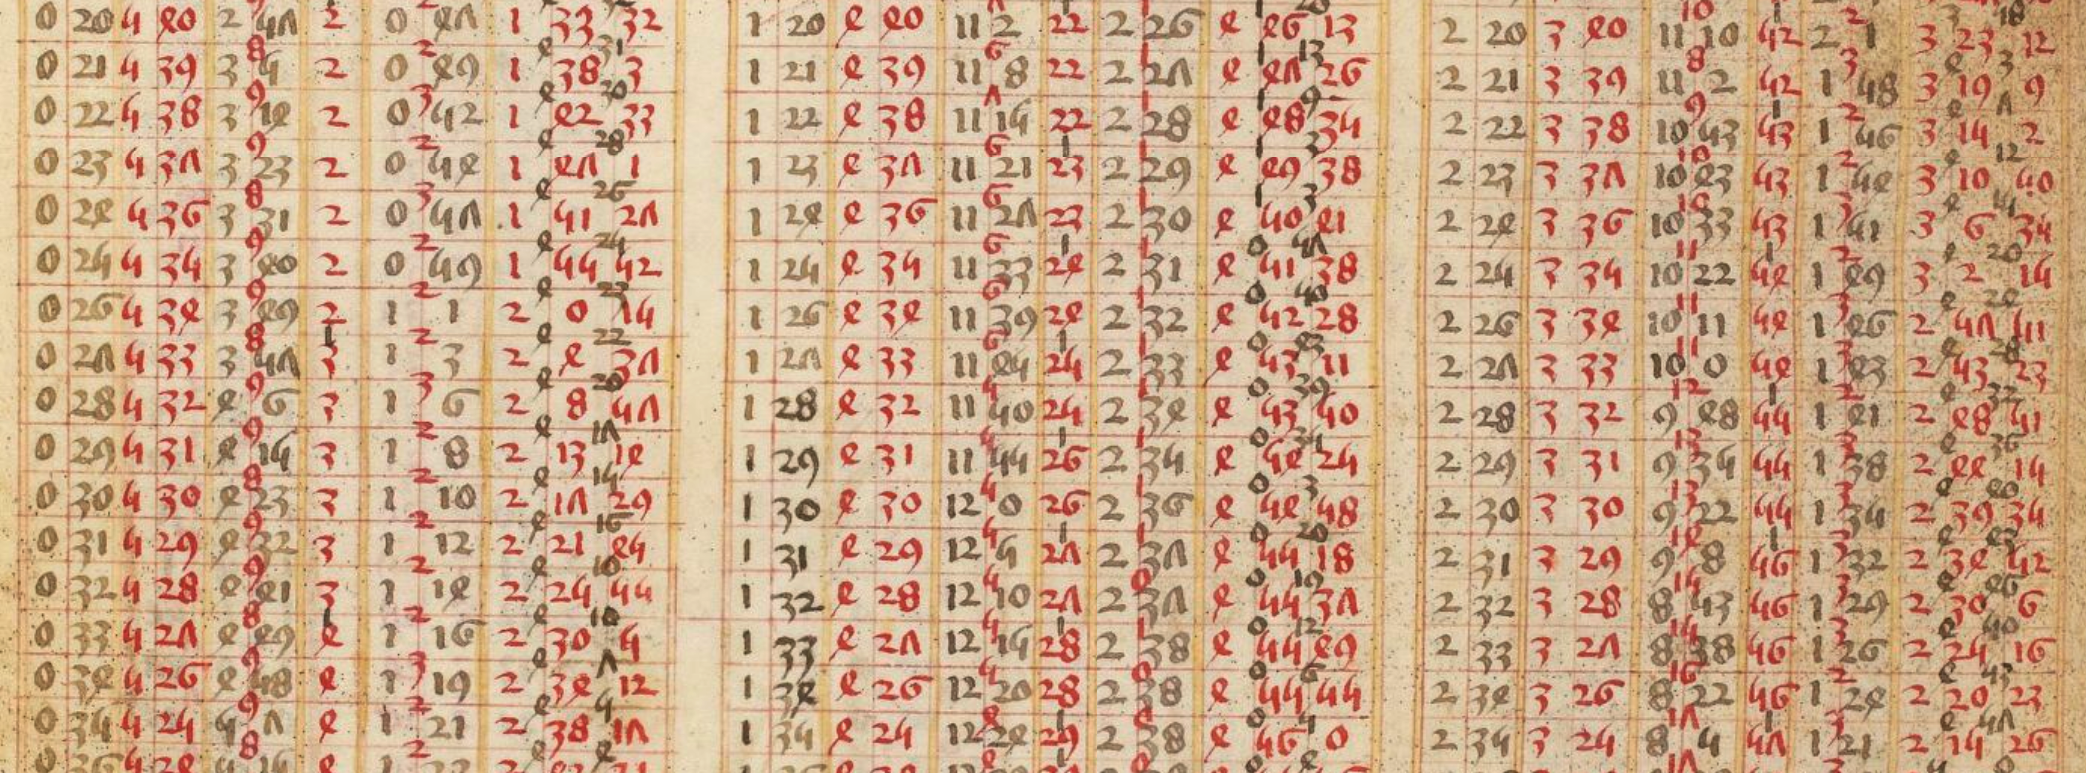
\includegraphics[width=12cm]{Images/Latin_14481.png}
	\caption{BnF, Département des manuscrits – Latin 14481, f.~81v – Équation de la Lune}
\end{figure}

Les tables astronomiques de calcul constituent ainsi un matériau indispensable pour l'étude~: elles ont par conséquent été choisies pour former le cœur du corpus de recherche de \dishas. Les tables, par la dimension d'abstraction mathématiques qu'elles recquièrent, sont particulièrement marquées par les différentes influences intellectuelles de ceux qui les ont composées. Plutôt que d'être recalculées entièrement, les astronomes les adaptaient à leurs besoins~; ainsi, elles sont révélatrices du milieu intellectuel de leur créateur.

Pour le chercheur moderne, une table astronomique représente une fonction mathématique (par exemple : \emph{f(x) = ax + b}), dont les valeurs \emph{a} et \emph{b} sont des constantes et dont le résultat est calculé de manière incrémentale pour chaque valeur de \emph{x}. Une table de multiplication est en ce sens comparable aux tables de calculs~: sans disposer d'information supplémentaire, l'enchainement des nombres peut suffire à déterminer de quelle table de multiplication il s'agit. Ainsi, la disposition des nombres dans les cases, la mise en page du tableau et les nombres en eux-mêmes portent des informations sur les pratiques des savants~: il est possible d'y déceler des variations dans les procédures ou dans les formules, ou encore d'observer des variations dans les types de nombres et dans les usages arithmétiques.\\

L'intégralité des sources primaires astronomiques a vocation à être progressivement intégrée aux interfaces et outils développés par \dishas, et certains documents réalisés par les chercheurs de l'équipe pourraient d'ores et déjà être mis à disposition au sein de la plateforme en tant que contenu explicatif. Toutefois, dans un souci d'inclusion, il est important que les productions scientifiques des projets partenaires soient également exposées au sein de l'interface de \dishas, Les tables de calcul sont donc, par leur contenu essentiellement numérique, un élément fédérateur des différentes cultures représentées dans le projet~; il faut cependant envisager dès à présent, dans la conception de la plateforme, les espaces et les fonctionnalités qui pourront être dédiées aux sources non-tabulaires.

		\subsection{Les paramètres}
			\subsubsection{Type de paramètres}
Les paramètres correspondent à la granularité la plus fine du corpus de \dishas: ils représentent les données numériques qui interagissent avec la fonction sous-jacente d'une table. Ces paramètres sont tantôt visibles au sein même de la table, tantôt présents implicitement dans le rapport des valeurs numériques entres elles. Dans \dishas, on distingue trois types de paramètres~: les paramètres astronomiques (ou \eng{set} de paramètres), les paramètres mathématiques et les paramètres \g{contextuels}. Ces derniers sont les valeurs numériques liées à un lieu ou une période, une table astronomique étant généralement calculée pour un endroit en particulier. Les paramètres mathématiques sont des artifices mis en place par les astronomes pour faciliter les calculs. Ils se divisent en deux groupes~: les \eng{shift}, décalage des nombres d'une colonne, et les \eng{displacement}, ajout d'une constante à tous les nombres de la table pour éviter les opérations avec des valeurs négatives.

Les paramètres astronomiques sont les nombres –~visibles ou non dans une table~– qui se retrouvent dans des dispositions analogues au sein des tables de calcul du même type. De façon similaire qu'il est possible de déduire de l'enchaînement des nombres qu'il s'agit d'une table de multiplication, la présence de certains paramètres astronomiques indique qu'une table a trait à un objet astronomique en particulier~: l'apparition du paramètre \emph{4,56} est, par exemple, révélateur du fait qu'il s'agit d'une table concernant la Lune. Le plus souvent, ces paramètres sont combinés en \eng{sets}~: le rôle des chercheurs est, entre autres, de comprendre comment ces assemblages numériques ont été composés et adaptés par les acteurs de l'époque.

			\subsubsection{Spécificité et intérêt des paramètres}
Le projet \dishas avait initialement été envisagé comme une base de données de paramètres astronomiques~: en effet, pour un grand nombre de chercheurs, les paramètres astronomiques sont des marqueurs forts pour déterminer la provenance d’une table. L’étude de la répartition de l’apparition de certains paramètres permet notamment de reconstituer les flux d’échanges intellectuels, le long de la route de la soie par exemple. Les paramètres sont un instrument pour l'identification d'une tradition astronomique~: dans le cas de l'histoire de l'astronomie, la donnée mathématique s'associe au contenu textuel pour révéler le contexte culturel et l'environnement historique d'un document.

La description de ces paramètres est centrale pour la recherche en astronomie ancienne. \dishas doit avant tout assister les chercheurs du projet dans leur étude~: une attention toute particulière doit donc leur être portée au sein de l'interface. La nature de ces paramètres a déjà fortement façonné les réalisations construites dans le cadre du projet~; ces paramètres, bien que parfois sous-entendus par les scribes, doivent être transcrits explicitement dans la base de données afin d'être pris en compte dans des traitements statistiques. Ils sont la clef de compréhension des tables, nécessaires à l'analyse du corpus. Les paramètres constituent assurément une donnée centrale, mais, par leur nature, ils peuvent rester hermétiques pour de nombreux publics. En ce sens, un effort de médiation doit être fourni pour assurer la valorisation de cette donnée.

\clearemptydoublepage

\chapter{Numérisation et accueil de la donnée}
	\section{Modélisation de la donnée}
La modélisation de données est une étape fondamentale pour tout projet en humanités numérique~: elle est l'occasion de définir précisément les enjeux du travail de recherche\footnote{\g{Objet construit, le modèle, par la formalisation qu’il nécessite, oblige l’historien à une plus grande rigueur dans l’expression des hypothèses interprétatives qui le sous-tendent.}~ \cite[p.~25]{fargeGoutArchive1997}} et de considérer les sources documentaires étudiées dans ce qu'elles ont de commun. La modélisation est également le lieu privilégié du dialogue entre ingénieur et chercheur, les compétences de chacun étant sollicitées pour la création d'une donnée rigoureuse scientifiquement et utilisable informatiquement\footnote{\cite[§~17-18]{clavertHistorienProgrammeur2012}}. Dans la perspective de construire une interface en adéquation avec la donnée, il est primordial de maîtriser le modèle dans les subtilités qu'il peut présenter. Les intentions comme les implications de celui-ci doivent être intégrées à la réflexion~; en fonction de la conceptualisation des données, les possibilités de visualisations ne sont pas équivalentes.\\

Dans le cadre du projet \dishas, les exigences quant à la polyvalence des données et à l'intégration culturelle ont présidé à l'établissement du modèle~: il était important que la structure de la base de données soit flexible, dans le but de publier et d'interroger des sources de nature diverses. Un des choix de modélisation principaux concerne la granularité donnée à la base~: comme il a déjà été mentionné, la table constitue l'unité fondamentale du modèle. Autour d'elle s'articulent les entités \Oi, le témoin, et \eng{Edited text}, l'édition. Le modèle de données se fonde sur cette dichotomie~: une partie du modèle est orientée vers les enjeux scientifiques liés à l'édition d'une table et à son contenu numérique, l'autre partie portant sur la description historique des sources. Ces deux parties se rejoignent grâce au lien existant entre document original et édition de ce document. Cette bipartition est caractéristique du travail de recherche des membres de \dishas, touchant à des disciplines diverses, comme la codicologie et les mathématiques anciennes.

\begin{figure}[h!]
	\centering
	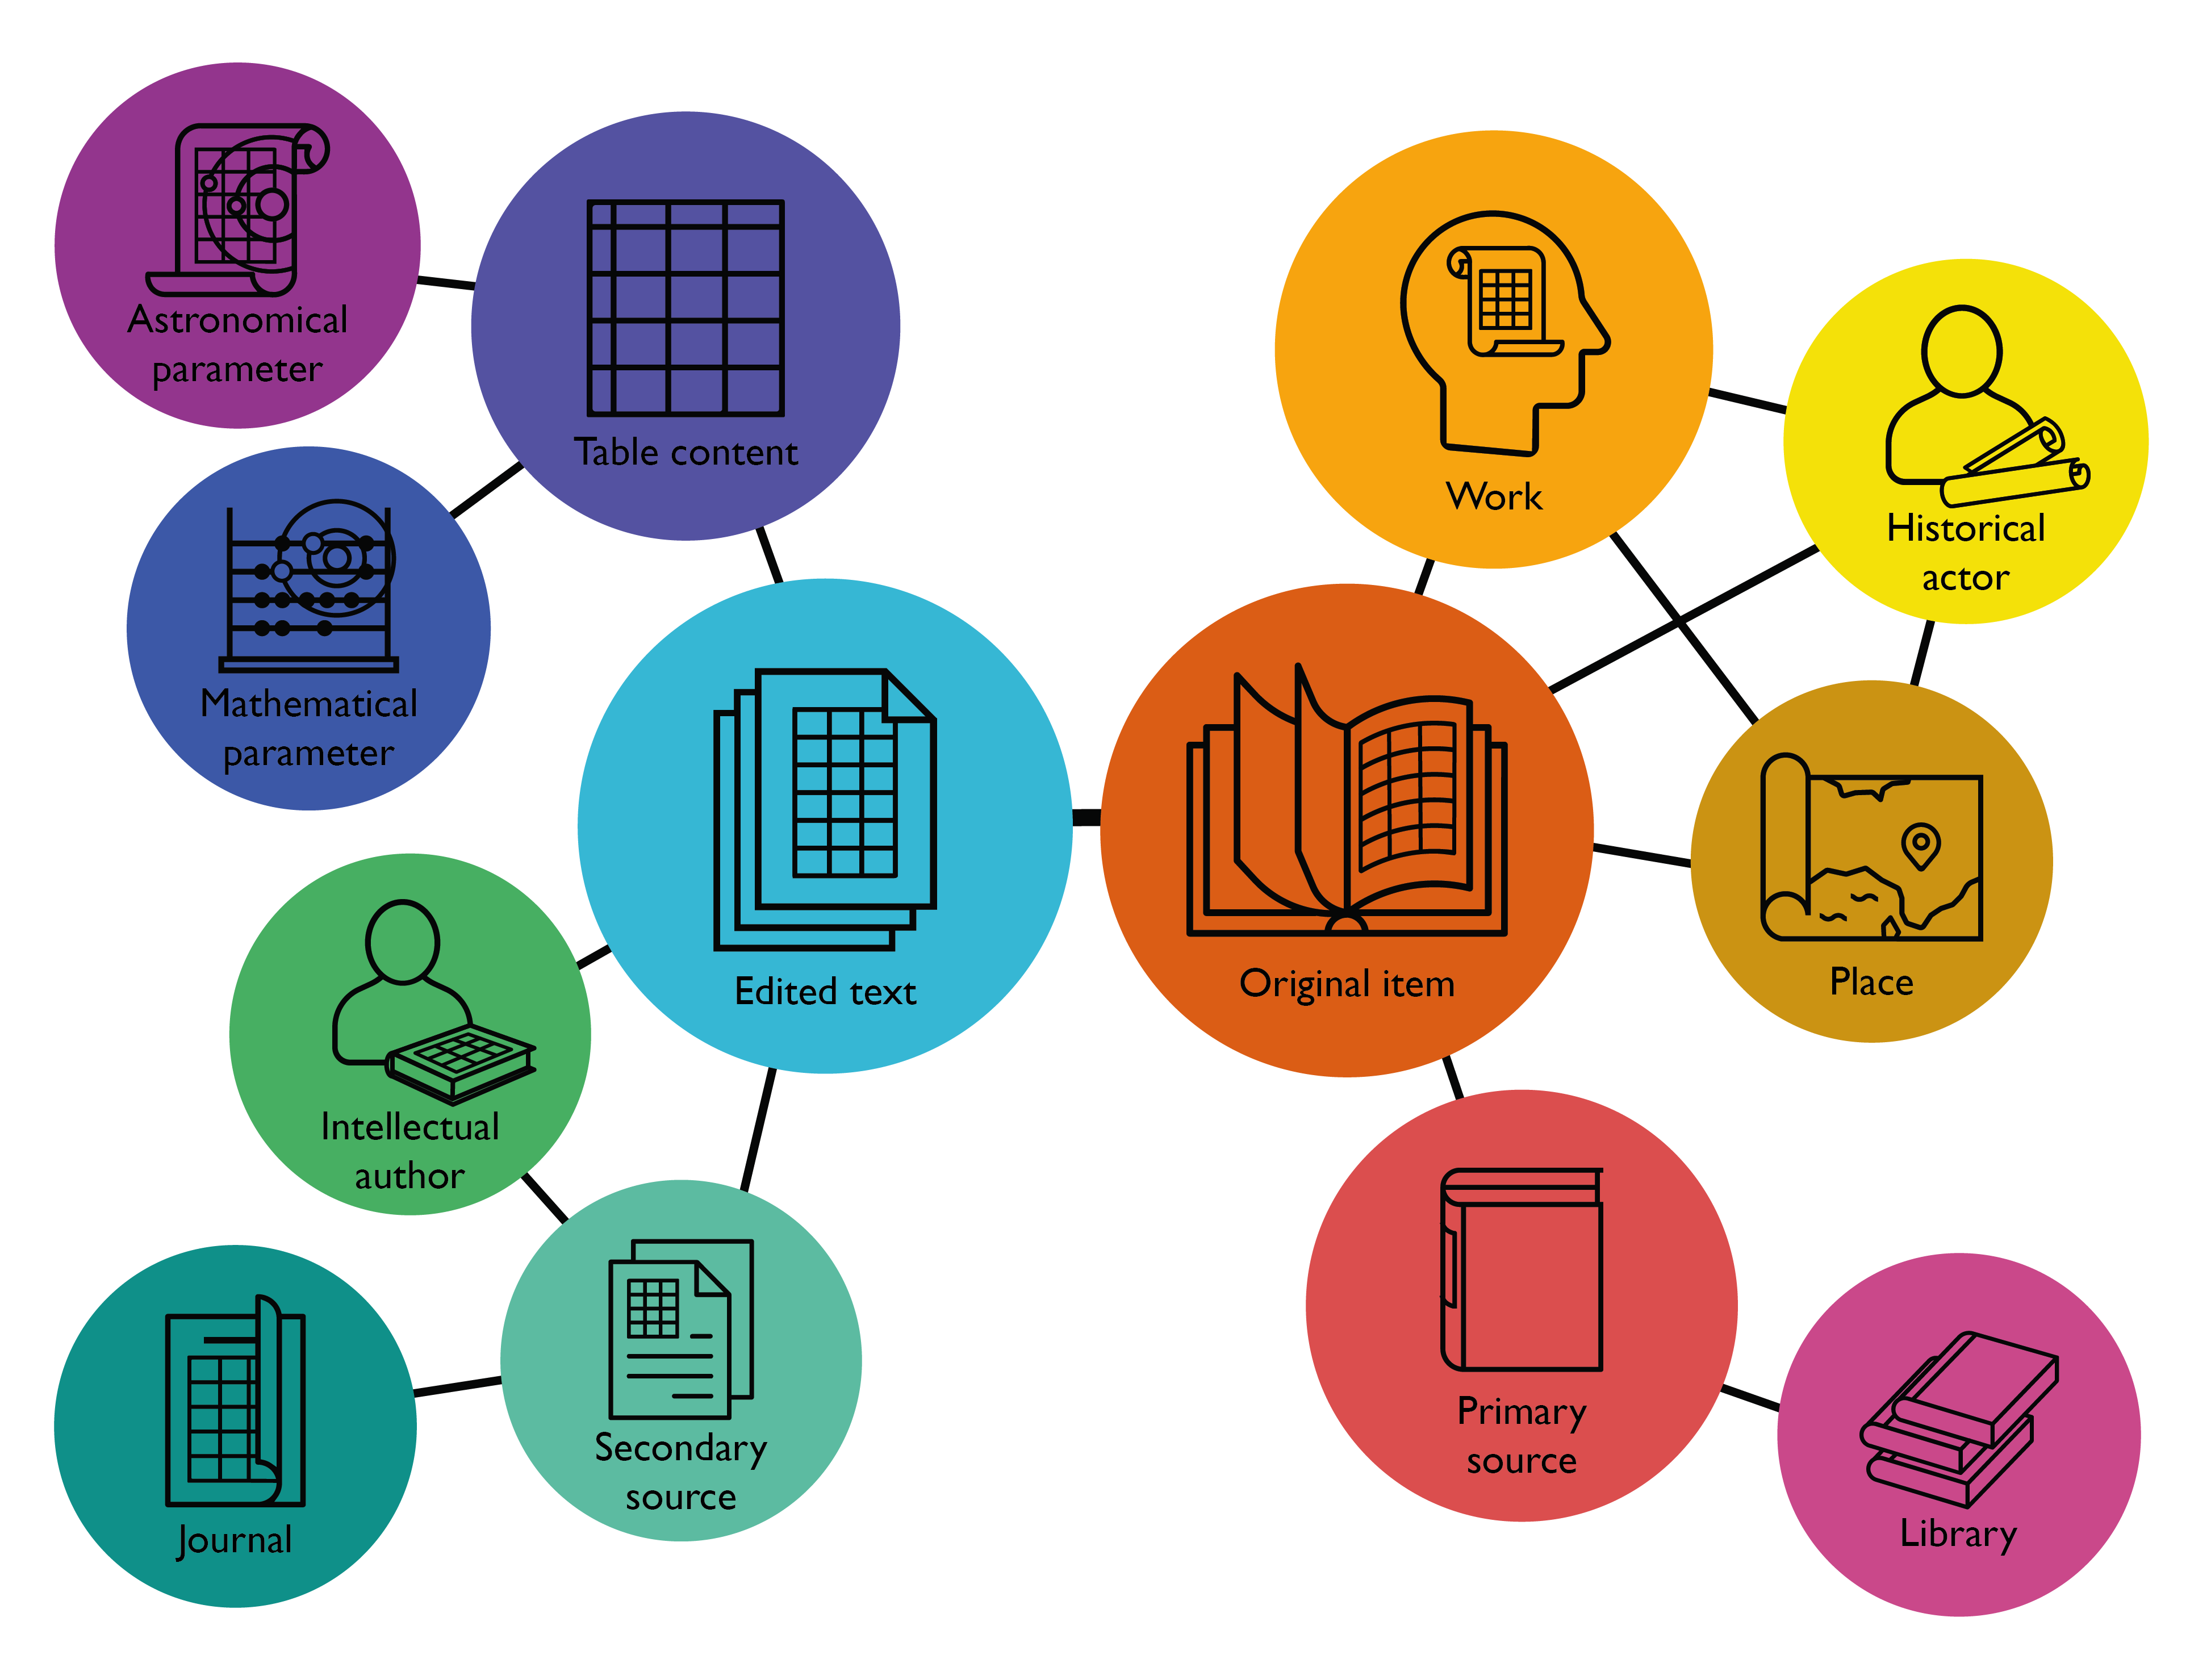
\includegraphics[width=12cm]{Images/Modele-de-donnees.png}
	\caption{\label{Modelisation}Modèle conceptuel de la base de données de \textsc{dishas}}
\end{figure}

La souplesse du modèle a été garantie grâce à la distinction faite entre contenu intellectuel et métadonnées de catalogage. Cette structure s'inspire notamment des spécifications du \frbr, où sont différenciés œuvre, expression, manifestation et item. Cette séparation implique notamment que l'édition soit partitionnée entre informations relatives au contexte éditorial d'une part, et valeurs numériques transcrites dans l'édition d'autre part. De la même manière, une source historique est découpée entre sa manifestation matérielle (incunable ou manuscrit), le contenu intellectuel qu'elle contient (les différentes œuvres qu'on peut y trouver) et les différents exemplaires de tables présents dans son corps. Cette finesse de description permet par exemple d'analyser en détail la composition intellectuelle d'un manuscrit donné, ou encore d'associer plusieurs ensembles tabulaires à une même édition. Par la généralisation du modèle, il est ainsi possible d'intégrer toutes les particularités du matériau à numériser.

		\subsection{Les sources historiques}
			\subsubsection{L'item original}
L'\oi représente une partie du contenu de la source primaire qu'il est possible de considérer indépendamment. Il peut être constitué d'un diagramme, d'un texte ou encore d'une table~; dans la base, il est associé à une métadonnée de type –~tabulaire, diagrammatique ou textuel~– qui en précise la nature. Toutefois, les interfaces et outils développés sont pour l'instant uniquement destinés aux tables astronomiques.

Afin d'expliciter la place de l'\oi au sein la base de données, un rapprochement peut être fait avec le genre du poème~: un poème, en effet, constitue une unité textuelle qui possède sa propre cohérence. Il a été composé –~généralement par un auteur unique~– pour apparaître à l'intérieur d'un recueil réunissant plusieurs poèmes~: ce recueil est l'œuvre intellectuelle d'où provient le poème. Il peut faire l'objet de plusieurs éditions, où la mise en page et même le texte peuvent varier. Ces éditions correspondent aux sources primaires du modèle conceptuel~; celles-ci peuvent contenir ou non l'intégralité des poèmes du recueil. Les éditions, quand elles prennent la forme d'une anthologie, mêlent les poèmes de plusieurs auteurs et d'œuvres différentes~; deux poèmes d'un même auteur provenant de recueils séparés pouvant ainsi se trouver rassemblés.

L'\oi est à la fois lié à une œuvre, c'est-à-dire à une production intellectuelle intangible dont il est une manifestation, et à une source primaire, objet matériel dont il est une partie. L'œuvre et la source ne sont pas associées dans la base de données, une source, de nature souvent composite, pouvant contenir plusieurs œuvres différentes. En outre, les informations concernant la langue et l'écriture sont également liées uniquement à l'item, parce qu'une œuvre peut par exemple se manifester dans différentes langues, ou encore qu'un manuscrit peut être copié dans plusieurs types d'écriture\footnote{La normalisation des langues et des écritures dans la base se fonde sur le standard \textsc{iso} facilitant ainsi un travail d'alignement ultérieur.}. De la même manière, le scribe et le lieu de copie d'une source ne sont liés dans la base de données qu'à l'\oi, permettant ainsi de signaler avec précision quels passages d'une source primaire ont été rédigés par un même acteur historique ou à un même endroit. Ainsi, l'item centralise les informations au niveau le plus fin de la description, permettant de cette manière de caractériser l'ensemble des sources historiques avec davantage de finesse.

			\subsubsection{Entités associées}
Deux entités majeures se distinguent dans leurs corrélations à l'\oi~: ce sont l'œuvre et la source primaire. La source primaire dans \dishas correspond à un manuscrit ou un incunable, dans lequel peut être trouvé un \oi. Le rôle de cette entité dans la base de données est d'identifier de manière univoque le document en lui-même, de manière à pouvoir retrouver facilement son lieu de conservation, dans l'éventualité d'une étude approfondie. Une attention particulière a été portée à la matérialité du texte, chaque item étant repéré précisément au sein de sa source, de manière à pouvoir mener des investigations sur la composition d'un manuscrit et retracer l'élaboration progressive de l'objet. Comme dit précédemment, une source primaire n'est pas associée à un lieu dans la base, il est possible de connaître l'endroit de sa copie uniquement par le biais des \ois: ce choix de modélisation a constitué une difficulté à contourner dans l'élaboration de certaines visualisations.

L'œuvre au sein de la base de données correspond à une création intellectuelle distincte~: ce sont généralement des écrits théoriques contenant des textes, des diagrammes et des tables astronomiques. Une œuvre est identifiée grâce à son titre, ou à défaut, son incipit. En outre, l'œuvre est reliée dans la base à un acteur historique –~son créateur~– et au lieu de sa conception. Comme il a déjà été mentionné, le contenu d'une œuvre se retrouve de manière plus ou moins complète à l'intérieur des sources primaires qui la contiennent. De même qu'il est intéressant, dans une perspective de bibliographie matérielle, de considérer l'agencement des œuvres au sein d'une même source, les variations de complétude d'une œuvre au sein des sources primaires peuvent faire l'objet d'un examen approfondi. Grâce à une modélisation centrée sur l'\oi, ces informations sont contenues dans la base de données et peuvent être mises au jour.

Par ailleurs, le concept d'œuvre pose plusieurs difficultés et peut être sujet de débat, compte tenu des différentes approches de recherche~: quels contours exacts peut-on donner à sa définition~? La traduction d'un écrit constitue-t-elle une nouvelle œuvre~? Comment considérer les \eng{marginalias} qui entourent le texte ou encore l'ajout d'une colonne à une table préexistante~? La réponse à ces interrogations est à la charge du chercheur~; le plus souvent, c'est l'importance des ajouts et des modifications qui distingue une œuvre originale, d'une simple copie ou transposition. Une traduction qui admettra des adaptations du document sur lequel elle s'appuie –~par exemple en changeant des paramètres en fonction du lieu de rédaction~– sera ainsi encodée dans la base en tant qu'œuvre indépendante. Cela peut occasionner des situations quelque peu paradoxales où une œuvre est associée dans la base à un traducteur, alors que seul l'\oi porte l'information quant à la langue de cette œuvre~: la souplesse du modèle de données rentrant ici en concurrence avec une représentation plus logique de l'information.

		\subsection{Structuration des données d'édition}
Le texte édité constitue le pendant de l'\oi au sein de la partie éditoriale du modèle de données. L'édition en tant que telle est divisée entre son contenu tabulaire (\eng{Table content}) et les métadonnées éditoriales (\eng{Edited text})~: cette distinction correspond entre autres à la nature de la donnée, l'entité \eng{Table content} ayant les caractéristiques d'une base de données orientée documents.

Le contenu tabulaire rassemble les données numériques de la table, définissant notamment les paramètres utilisés~; les métadonnées éditoriales concernent quant à elles l'auteur intellectuel de l'édition, le journal dans lequel elle est parue et le titre de la publication.

Plusieurs éditions peuvent être réalisées d'un même \oi, et une édition peut elle-même s'appuyer sur plusieurs éditions préalables. Le travail de transcription d'une table étant sujet à interprétation\footnote{Certaines tables, compte tenu du chevauchement des nombres ou encore de certaines graphies, comportent des incertitudes de lecture~; cette ambiguïté était probablement déjà présente chez les lecteurs médiévaux, il s'agit de ne pas l'effacer lors de la numérisation.}, il est ainsi considéré dans \dishas qu'une édition critique de plusieurs témoins constitue en réalité l'édition de plusieurs éditions. Une simple transcription constitue déjà en ce sens, une édition classique (éditions de type \textsc{a}, voir ci-dessous pour la définition).

			\subsubsection{Données éditoriales}
L'application Web du projet \dishas a été pensée de prime abord pour être une plateforme d'éditions de table\footnote{Projet qui a été écarté au profit d'une plateforme d'\eng{open data} pour ne pas rentrer en concurrence avec d'autres plateformes de publication en ligne.}, cet aspect de la recherche étant particulièrement important en astronomie ancienne. Toutefois, le modèle de données relatif aux éditions n'accueille en réalité que le contenu de la table, et non l'intégralité de l'article susceptible de l'accompagner. Le travail de modélisation s'est donc concentré sur la description des types d'éditions de table~; il en existe trois sortes au sein de la plateforme~:
\begin{itemize}
	\item Édition de type \textsc{a}~: s'appuyant sur un unique \oi, ce sont les éditions au plus proche du texte. Il n'est cependant pas possible de parler d'édition diplomatique dans la mesure où aucune donnée de mise en page n'est reproduite~;
	\item Édition de type \textsc{b}~: ces éditions reposent sur plusieurs éditions de type \textsc{a} mais aussi potentiellement de type \textsc{c}~; elles figurent donc un apparat critique.
	\item Édition de type \textsc{c}~: pour réaliser ce type d'édition, le chercheur récupère les paramètres d'une table témoin et recalcule l'ensemble de ses valeurs grâce à des modèles mathématiques contemporains. Ce type peut servir notamment à comparer les techniques arithmétiques anciennes et modernes, pour observer par exemple les variations de certaines constantes mathématiques.
\end{itemize}
S'il est prévu de pouvoir éditer des tables de manière nativement numérique grâce à l'interface de \dishas, une partie des éditions qui ont vocation à être intégrées à la base ont été déjà publiées sur papier. C'est pour cette raison que les entitées \eng{Journal} et \eng{Secondary source} ont été ajoutées au modèle de données~; elles signalent d'où provient une édition, permettant de retrouver le matériau de départ pour l'étudier plus avant. Pour les sources primaires et secondaires, \dishas a donc destination à servir de portail, plus que de plateforme de consultation.

			\subsubsection{Données astronomiques}
Les données liées aux aspects mathématiques des tables sont encodées dans la partie éditoriale de la base, car elles constituent une interprétation moderne des raisonnements arithmétiques des acteurs de l'époque~; seul le type de table est associé aux enregistrements d'\eng{edited texts} comme d'\ois. On dénombre 70 types de tables au sein de la base~; ils représentent la fonction sous-jacente à une table, son objectif de calcul (par exemple déterminer le mouvement moyen d'un astre). Le type de table est l'entité qui centralise les informations relatives au contenu mathématique et astronomique d'une table, que ce soient les paramètres ou les définitions de modèles.

				\paragraph{\label{Parametre}Les paramètres}
Les paramètres, en particulier les paramètres astronomiques, constituent les entités les plus complexement décrites dans le modèle de données~; le schéma ci-dessous représente les tables de la base de données utilisées pour la modélisation des paramètres astronomiques. La multiplicité de ces tables permet notamment d'effectuer des traitements mathématiques automatisés sur les données numériques de la base, mais cette finesse de description est également utile aux chercheurs dans leurs travaux et doit être exposée au mieux dans les interfaces graphiques de la plateforme.

\begin{figure}[h!]
	\centering
	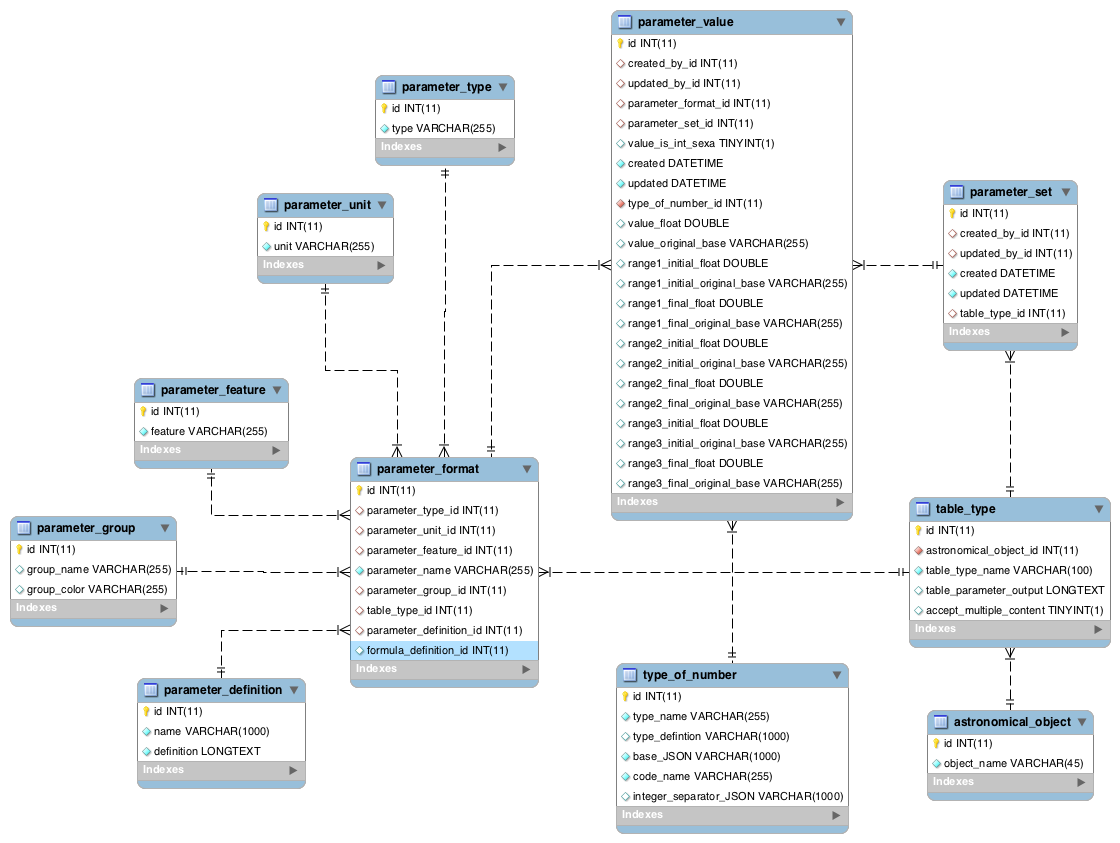
\includegraphics[width=13cm]{Images/Astronomical_parameter.png}
	\caption{Visualisation de l'architecture des données de paramètres astronomiques dans la base}
\end{figure}

Toutes les tables représentées ci-dessus fonctionnent ensemble~: la table \eng{Parameter type} par exemple, renseigne sur le mode d'apparition d'un paramètre dans une table (explicite, implicite ou mixte\footnote{Visible au sein de la table (explicite) ou contenu implicitement dans le rapport des valeurs de la table entre elles (implicite). Le type mixte correspond généralement à un cas où le paramètre est exprimé explicitement, mais où la disposition bouleversée de la table en rend l'identification malaisée}), tandis que la table \eng{Parameter feature} indique le nombre d'arguments admis par le paramètre (simple, double, parfois triple). La table \eng{Parameter group} réunit quant à elle les paramètres fonctionnant ensemble, là où la table \eng{Parameter set} rassemble les paramètres permettant de décrire un type de table\footnote{Le terme \g{set de paramètre} est également utilisé pour signifier \g{paramètre astronomique}~: ces deux significations désignent des réalités distinctes. Un paramètre astronomique, à l'instar de \emph{4,56}, correspond à une valeur définie~; un set de paramètre est l'ensemble des variables nécessaires au calcul d'une table selon un modèle précis, les valeurs n'en sont pas définies.}. Enfin, la table \eng{Parameter format} agrège toutes ces informations pour les associer à un enregistrement de la table \eng{Parameter value} qui instancie une valeur à un paramètre, conservée à la fois sous sa forme originale et sous sa forme fractionnaire afin d'effectuer des calculs.

Si les tables de paramètres sont aussi nombreuses, c'est pour assurer l'encodage exhaustif toutes les informations implicitement contenues dans une table astronomique. Il est important de rendre accessibles l'ensemble de ces données au public de la plateforme, en s'assurant de fournir une interface adaptée pour leur présentation.

				\paragraph{\label{FormulaDefinition}Les modèles de tables}
Les modèles –~contenus dans la table \eng{Formula definition} de la base de donnée\footnote{Pour une représentation de la base de données présentant toutes les tables concernant l'histoire de l'astronomie, voir annexe \pageref{BaseDeDonnee}.}~– reposent en grande partie sur la définition de ces paramètres. Ils sont une forme modernisée des canons, résumant à l'aide d'une formule mathématique la fonction sous-jacente à une table. Un modèle est défini pour un type de table en particulier –~par exemple les tables de vélocité solaire~– et requiert un set de paramètre précis –~par exemple la distance Terre/Soleil ainsi que la valeur de l'excentricité solaire. En revanche, un même type de table peut admettre plusieurs modèles~; autrement dit, pour le calcul d'une même donnée astronomique, plusieurs méthodes mathématiques sont possibles.

\begin{figure}[h!]
	\centering
	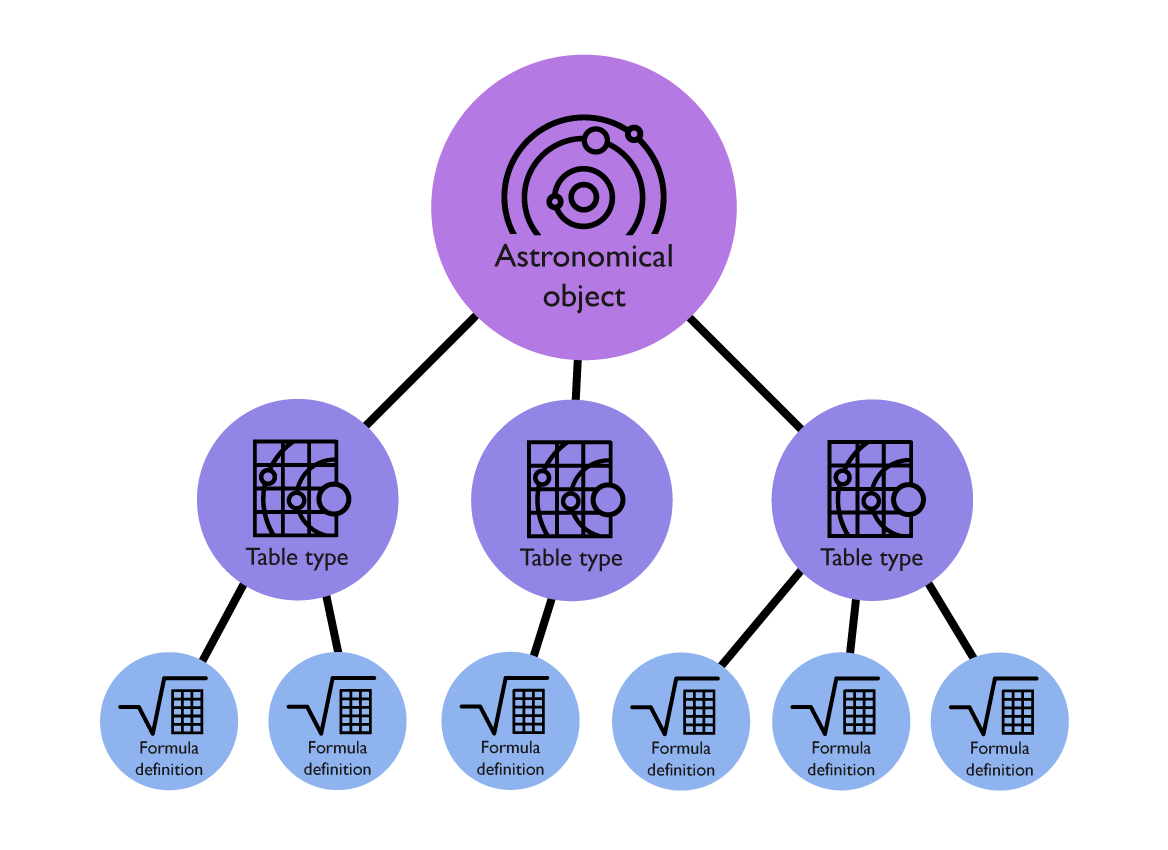
\includegraphics[width=11cm]{Images/Table-models.png}
	\caption{Exemple de structuration de modèles mathématiques dans la structure de données}
\end{figure}

La définition de ce genre de modèles est très utile pour comprendre la manière dont ont été composées les tables astronomiques~: ils permettent notamment de recalculer les valeurs d'une table et de les comparer avec les valeurs telles que présentes dans une source, afin de révéler les différences de conception mathématiques entre nos méthodes modernes de calcul et les techniques anciennes de computation. Ils peuvent également être utilisés pour aider à la saisie automatique de table, de manière à faciliter la transcription tout en révélant les zones où les formules arithmétiques contemporaines ne correspondent pas à la logique des savants passés. Enfin, en intégrant ces modèles à des réseaux de neurones entraînés, il est possible d'imaginer pouvoir aider à résoudre les équations sous-tendues à certaines tables, qui n'ont été élucidées jusqu'à présent\footnote{Les réseaux de neurones devrait réussir en réalité à \g{craquer} les tables, c'est-à-dire trouver toutes les fonctions, aussi complexes et invraisemblables soient-elles, qui reproduisent la même progression numérique que celle observée dans le contenu tabulaire. Le travail du chercheur sera de raffiner ces résultats pour trouver des estimations qui semblent les plus plausibles}.\\

Cette donnée, fruit de l'expertise des chercheurs du projet, constitue une porte d'entrée pour aborder l'histoire de l'astronomie. Seuls les administrateurs de la plateforme sont autorisés à rentrer au sein de la base de données des modèles de tables~: ils représentent donc une des valeurs ajoutées de \dishas, une ressource qu'il faut absolument valoriser auprès du public.

		\subsection{Développements futurs de la base de donnée}
Certaines évolutions ont été prévues pour la base de \dishas, en premier lieu l'ajout au modèle de données de tables décrivant les paramètres contextuels (liés au contexte historique et géographique d'une table)~: il existe d'ores et déjà dans la base les entités \eng{Calendar} et \eng{Era}, tâchées de décrire le système temporel utilisé par une table. Ces entités vont être rattachées au reste des tables dans des développements futurs.

En outre, les diagrammes et les textes pourront à terme être ajoutés en tant qu'enregistrements de la base de données mais ces modifications seront probablement réalisées par un autre groupe de recherche en histoire de l'astronomie, extérieur à l'Observatoire. Le modèle de données n'est donc pas entièrement arrêté, chose à prendre en compte lors des développements des interfaces.\\

Pour davantage d'informations sur le modèle de données, un glossaire des principales entités de la base de \dishas est disponible en annexes \ref{Glossaire}, à la page \pageref{Glossaire}.

	\section{Données de gestion et encodage de l'information}
		\subsection{Données structurelles}
			\subsubsection{Données non-\emph{manageables}}
Les tables de la base de données peuvent être rangées en deux catégories~: les tables de données modifiables par l'utilisateur, et les tables contenant des informations n'étant pas vouées à être remaniées. Ce dernier type assure, entre autres, la cohésion de l'encodage des métadonnées. C'est le cas par exemple des entités \eng{Script} et \eng{Language} qui centralisent tous les enregistrements de langues et d'écritures pouvant être utilisées au sein d'un \oi de la base. L'exhaustivité est assurée par le recours à un standard –~le standard \textsc{iso} en l'occurrence~– qui garantit de décrire tous les arrangements possibles de graphies et de vocabulaires, tout en facilitant un travail d'alignement ultérieur.

L'utilisation de normes permet en effet de renforcer la cohérence des métadonnées~; le risque peut être cependant de restreindre les chercheurs quant à l'encodage qu'ils souhaitent appliquer à leur sources. Il aurait ainsi été possible de calquer les données de lieux sur la base géographique de GeoNames, mais cela n'aurait pas permis, par exemple, d'ajouter des noms de lieux fictifs. Les données auxquelles l'utilisateur n'a pas accès doivent donc couvrir toutes les éventualités qu'il est possible de rencontrer dans les sources.

En outre, certains choix d'organisation du corpus ont été fixés dans la base de données, bien que leur modélisation eut pu être différente~: c'est le cas en particulier de la table \eng{Astronomical object} qui classifie tous les types de tables astronomiques en 11 groupes. Ces groupements ont été constitués au moment de la création de la base de données~; il s'agit donc de justifier et d'expliciter ces options de modélisations au sein même de l'interface afin qu'elles n'apparaissent pas comme arbitraires aux utilisateurs.

			\subsubsection{Données d'interface}
Un autre type de données structurelles a été intégré directement à la base, il concerne les éléments utilisés pour la construction de l'interface. Deux tables en particulier sont utilisées dans ce but~: la table \eng{User interface text} et la table \eng{Definition}. La première rassemble les textes destinés aux utilisateurs lors de leur navigation dans la plateforme, le texte d'introduction au projet comme les messages d'annonce pour la partie administrateur. Ces textes sont stockés sous format \html de manière à pouvoir être mis en forme dans une interface graphique et affichés de manière identique~: cette pratique s'inspire des \cms, à l'instar de Drupal ou Omeka, qui offrent ainsi une grande liberté de configuration, tout en conservant une interface graphique plus facile à manier par les utilisateurs.

La table \eng{Definition} quant à elle réunit les informations relatives à chaque entité du modèle de données concernant l'astronomie ancienne~: l'entité \Oi y est par exemple associée à une définition, à une couleur et à plusieurs variations dans l'écriture de son intitutlé\footnote{En \eng{camel case} pour l'utilisation \php (\g{originalText}) ou en \eng{snake case} pour l'intitulé dans la base de données (\g{original\_text}).}. En effet, y sont distingués le véritable nom de la table dans la base de données \textsc{sql} –~\eng{Original text}~– de celui utilisé au sein de la plateforme. Ceci permet une grande modularité des options de présentation et aide à la mise à jour pour le changement de la charte graphique entre autres.

			\subsubsection{Données utilisateurs}
Le dernier type de données qu'il est important d'aborder concerne les données générées à la création de comptes utilisateur~: elles constituent des renseignements sensibles, qui tombent sous le coup du \rgpd et qu'il faut traiter avec attention. Bien que les informations conservées sur les utilisateurs soient minimales –~nom, prénom, email et mot de passe crypté~– il est du rôle des ingénieurs de la plateforme de garantir la transparence quant à leurs utilisations, en même temps que d'en assurer le caractère privé.

Parallèlement, les concepteurs de \dishas doivent veiller à la qualité des données qui sont ajoutées~; en ce sens, il est essentiel de garder une traçabilité vis-à-vis des entrées et modifications dans la base. Ainsi, toutes les tables concernant les entités manipulables par les utilisateurs disposent de champs précisant la date et l'auteur de l'ajout, ainsi que les mêmes informations en cas de remaniement. Les données utilisateurs sont donc centrales dans la plateforme et doivent en conséquence être considérées attentivement dans leur utilisation.

		\subsection{Encodage et typologie de la donnée}
			\subsubsection{Permissivité du modèle}
L'élaboration d'un modèle de données ayant vocation à être inclusif peut entraîner des difficultés~: comment établir un cadre pour controller la qualité des données, sans pour autant dénaturer le matériau sur lequel elles s'appuient~? D'une part, il est important de pouvoir ajouter des données n'ayant pas le même niveau de précision descriptive, d'autre part, une certaine régularité et consistance est nécessaire pour traiter l'information, dans les interfaces comme dans leur exploitation scientifique.

Le caractère obligatoire d'une information n'est pas spécifié dans le modèle la base~; il a été stipulé en revanche dans la construction des interfaces de saisies. Cela signifie que certaines données ne peuvent être insérées, tant que certains champs n'ont pas été remplis. Par exemple, il est indispensable de renseigner les bornes temporelles (\eng{Terminus Post Quem} et \eng{Terminus Ante Quem}) d'une œuvre lors de son ajout. L'éventuelle absence d'information exacte est prise en compte par la possibilité d'indiquer une période et non une donnée ponctuelle. Cela permet \eng{a posteriori} de faire des estimations sur les périodes les plus florissantes intellectuellement. De la même manière, si le lieu de copie exact d'un \oi n'est pas connu, il est possible d'indiquer, pour le renseigner, le nom d'un pays ou d'une région plutôt que celui d'une ville\footnote{Il n'est cependant pas obligatoire de renseigner un lieu lors de l'ajout d'un \oi.}.

En revanche, il ne faut pas que les exigences de visualisations prennent le pas sur l'exigence scientifique~: les modalités d'encodage et les objectifs de traitement de la donnée s'influencent, mais ce sont les ambitions de recherche qui doivent avoir la haute main sur la nature des données. Dans la conception des interfaces, il faut donc savoir composer avec l'absence, tout en incitant les chercheurs à produire la donnée la plus complète possible.

			\subsubsection{Encodage de la donnée en fonction de son utilisation}
Le format de stockage qui a été choisi pour \dishas est celui de la \bdd relationnelle. Ce genre de \bdd a l'avantage d'éviter les écueils de répétition de l'information et de pouvoir être maintenu facilement, dans la mesure où il est bien connu des directions de systèmes d'information. Pourtant, il ne constitue pas le format le plus adapté pour tous les types de matériau à intégrer à une base de données. Les formats \xml et \json offrent par exemple plus de flexibilité et d'autonomie pour la constitution d'une base~; ils sont également plus indiqués pour la description de matériel textuel. Plusieurs solutions ont été déployées dans le cadre de \dishas pour pallier l'insuffisance du format relationnel de la base de données.

Les tables astronomiques, tout particulièrement, ont reclamé un traitement spécifique pour leur incorporation dans la \bdd. Comment encoder un tableau de nombres, mis en page de façon complexe, à l'intérieur d'une ou plusieurs chaînes de caractères~? Le format \json a été préféré au \xml, notamment pour sa facilité de manipulation et sa compatibilité avec JavaScript, ce langage étant largement utilisé pour la construction de la partie frontale d'un site Web. La distinction dans le format de données a donc participé à la division conceptuelle des éditions de table~: le contenu numérique encodé en \json à l'intérieur de \eng{Table content}, et les métadonnées éditoriales au format plus classique dans la table \eng{Edited text}.

La conceptualisation du lien entre \oi et \eng{edited text} a également nécessité des ajustements. En effet, une édition pouvant elle-même être basée sur une édition, il était important de prévenir le risque de récursivité. L'architecture en graphe permet d'éviter ce genre d'aberration~; ainsi, la bibliothèque \eng{GraphTree}, développée pour les besoins du projet, a été employée pour vérifier qu'une édition ne fait pas référence à elle-même et du même coup, permettre de réaliser des visualisations de la parenté intellectuelle d'une édition.

	\section{Saisie de la donnée}
		\subsection{Interface administrateur}
La plateforme en ligne de \dishas dispose d'ores et déjà d'interfaces entièrement fonctionnelles~; c'est le cas de l'interface administrateur. Dans un site Web dynamique, l'interface administrateur –~ou \eng{back office}~– est la partie dédiée à la gestion des ressources. Les chercheurs disposant d'un compte\footnote{La sélection des chercheurs ayant accès au \eng{back office} est faite par Matthieu Husson, Benno Van Dalen et Clemency Montelle.} peuvent s'y connecter pour ajouter des données à la base, sans prérequis de connaissances en \sql ou autre langage de requête de \bdd. Elle s'oppose à l'interface utilisateur –~\eng{front office}~– qui est ouverte au public et qui fut l'objet de mon stage. Le rôle de l'interface administrateur est avant tout de faciliter la gestion des données pour les administrateurs, qu'il s'agisse de leur ajout, de leur modification ou de leur retrait. Elle constitue le socle sur lequel s'appuie la partie publique de l'application.

			\subsubsection{Rôle du \eng{back office}}
L'interface vise à assister les administrateurs dans la gestion de leurs données~: en ce sens, les pages de vues doivent identifier clairement les différentes entités de la base. Les chercheurs n'étant pas nécessairement familiers des \bdd, l'intuitivité des interfaces est l'une des priorités~; néanmoins, la simplicité d'utilisation ne doit pas se faire aux dépens de la compréhension du modèle de données sous-jacent. En effet, le \eng{back office} a aussi pour mission de garantir la qualité des données, en assistant les chercheurs dans le processus de numérisation~; l'explicitation du modèle conceptuel participe à cette qualité.

Il existe deux types de plateformes en ligne pour les données de recherche~: les plateformes où les données ont été moissonnées à partir de multiples systèmes d'information, et celles –~à l'instar de \dishas~– où l'intégralité du contenu numérisé a été créé par des chercheurs~: l'interface administrateur est l'instrument même de cette numérisation. L'objectif du premier type est le regroupement des ressources, l'ambition du second est la création d'un corpus qualitatif. La normalisation et le contrôle des données est donc du cœur du projet \dishas et l'interface administrateur doit aider dans cette mission.

Plusieurs fonctionnalités ont été mises en place dans ce but~: l'appel à des bases de référentiels comme le \viaf ou l'\isni (pour l'ajout d'acteurs historiques et de bibliothèques)\footnote{Ces référentiels servent également à valider la cohérence des \eng{inputs}.}, des procédures de vérification à la soumission de formulaires ou encore l'obligation au remplissage de certains champs. La manière dont l'interface est construite accompagne le chercheur dans l'insertion des données~; pour l'ajout d'une nouvelle édition par exemple, les informations à renseigner sont réparties dans plusieurs formulaires successifs, chacun conditionnant les champs à remplir dans le suivant.

Une des finalités de la création de ces données est leur publication au sein de l'interface publique~; la mise en ligne étant un objectif du travail de recherche en soi\footnote{\g{Il est ainsi désormais entendu que l’obtention du financement d’un programme de recherche collectif temporaire, notamment de l’ANR, dépend fréquemment de la mise en œuvre, et plus encore de la mise en ligne, de « données » et de « corpus », destinées à la fois à être les instruments et les résultats de l’opération de recherche elle-même.} \cite[§~2]{potinInstitutionsPratiquesArchives2011}}. Toutefois, certaines données ne sont prêtes à la publication qu'à l'issue d'un examen attentif de la part du chercheur~; deux états de travail ont donc été créés, un état \g{public} et un état \g{ébauche}. Les administrateurs de la base ont ainsi la possibilité de différer la mise en ligne d'un document, s'ils estiment que le processus de numérisation n'est pas terminé.

			\subsubsection{Structure de l'interface}
La structure du \eng{back office} est calquée sur celle de la \bdd. Sur la page d'accueil, l'utilisateur peut trouver la liste de toutes les entités auxquelles il a accès. Ces entités sont rassemblées dans des groupes cohérents, reprenant le modèle de données~:

\begin{itemize}
	\item Entités centrales~: \Oi, \eng{Edited text} et \eng{Table content}~;
	\item Celles liées aux sources historiques~: \eng{Primary source}, \eng{Work}, \eng{Historical actor}, \eng{Place} et \eng{Library}~;
	\item Celles liées à l'édition~: \eng{Intellectual author}, \eng{Secondary source} et \eng{Journal}~;
	\item Celles liées au contenu tabulaire~: \eng{Astronomical parameter} et \eng{Mathematical parameter}.
\end{itemize}

Chacune de ces entités donne accès à une page de liste de l'ensemble de ses enregistrements, ainsi qu'à des pages dédiées à chacun d'entre eux. La partie administrateur constitue en ce sens une interface graphique pour la base de données, les administrateurs pouvant accéder et modifier les ressources qu'ils ont ajoutées et parcourir celles ajoutées par d'autres~; l'autre fonctionnalité principale étant bien sûr l'insertion de données.

Aucune simplification vis-à-vis de la structure de données n'a été effectuée. Les ajustements relatifs à l'interface ont été concentrés sur la cohérence dans la navigation. Plusieurs niveaux de détails sont disponibles pour la visualisation des ressources~: une vue d'ensemble –~sur la page d'accueil~– listant toutes les entités importante de la base, des pages de listes détaillant tous les enregistrements pour une entité donnée, et enfin, des pages individuelles pour la visualisation des métadonnées relatives à un enregistrement unique. Ces différentes granularités de vues offrent plusieurs manières d'aborder les données~: pour aider encore à leur appréhension, des visualisations graphiques ont été incorporées, sous forme de carte et de graphe\footnote{Voir en annexes \ref{BackOffice}\xspace les captures d'écran de l'interface administrateur.}.

		\subsection{\label{DTI}Saisie assistée de tables astronomiques : présentation de DTI}
L'édition numérique de tables a fait partie, dès les prémisses du projet, du cahier des charges. En effet, les tables astronomiques constituent à de nombreux points de vue des objets complexes, dont l'édition, autant électronique que papier, soulève de nombreuses problématiques. La table constitue l'unité fondamentale du corpus de recherche~; à ce titre, l'élaboration d'outils dédiés à leur numérisation est une des conditions à l'obtention d'un corpus abondant. La création d'une interface pour assister à leur saisie fut donc l'un des objectifs de l'équipe technique du projet.

			\subsubsection{Choix du développement d'un outil sur mesure}
Plusieurs exigences techniques se sont dessinées des volontés de l'équipe de recherche. Elles visaient d'une part à faciliter la saisie du contenu tabulaire –~quelque soit son format et sa provenance~– et d'autre part à intégrer des outils pour le traitement de ce contenu~: remplissage semi-automatique grâce à des formules mathématiques intégrées, aide à la vérification des valeurs tabulaires, instruments de conversion et manipulation numérique, génération d'apparat critique.

De nombreux outils, existants antérieurement au projet, répondaient en partie aux exigences de développement d'une interface de saisie de table. Dans le domaine des humanités numériques en effet, de nombreuses applications sont dédiées à la transcription de sources historiques\footnote{On peut citer Transkribus, Recogito, \eng{From The Page} et bien d'autres.}, toutefois la plupart s'appuient sur des versions numérisées des sources. Dans \dishas en revanche, les tables du corpus ne disposent pas nécessairement de numérisation, et une importante partie des ressources à transcrire comprend des tables déjà éditées sous format papier. Pour ces dernières, l'interface de saisie a principalement vocation à rendre la numérisation plus rapide. D'autres outils, pour l'édition ou la conversion de nombres, préexistaient également au projet, mais le format tabulaire des ressources et la présence de systèmes numériques très particuliers\footnote{Notamment des systèmes \g{décimaux historiques} \eng{fen} et \eng{miao} chinois.} rendaient impossible leur utilisation dans le cadre de \dishas. Les spécificités du corpus ont donc amené à la création d'une interface sur mesure, plutôt qu'à l'agrégation d'outils existants.

La conception en interne de cette interface –~appelée \dti~– a également permis de réaliser une application intégrable directement au site Web de \dishas. Dans un contexte où la plupart des services sont disponibles en ligne, un logiciel à télécharger aurait constitué une difficulté supplémentaire à la numérisation du corpus. De plus, \dti, par sa portabilité et sa relative facilité d'utilisation\footnote{L'interface s'inspire largement du logiciel Excel.}, offre la possibilité à des non-spécialistes de saisir des tables déjà publiées, afin de décharger quelque peu les chercheurs du travail de numérisation.

			\subsubsection{Fonctionnalités de DTI}
\dti rassemble aujourd'hui de nombreuses fonctionnalités, au sein d'une interface conçue pour être le plus intuitive possible. Après avoir renseigné les dimensions de la table (nombre de colonne et de rangées), un tableau vide –~semblable à une feuille de tableur~– est généré.

Le remplissage des cellules du tableau peut être réalisé de plusieurs façons. La méthode la plus simple est de recopier individuellement la valeur de chaque cellule, mais il est possible de ne renseigner que certaines valeurs et de laisser les outils d'interpolation remplir les cases intermédiaires. Les modèles de tables peuvent également être utilisés pour des modalités d'auto-complétion~: en donnant les valeurs des arguments, \dti est ensuite capable de calculer les valeurs des celulles de la tables, selon la fonction définie dans le modèle. Chaque cellule doit ensuite être validée individuellement par l'utilisateur, de manière à assurer la qualité de la transcription. Tout état d'avancement peut être sauvegardé en tant que brouillon, tant que l'utilisateur estime que le travail de numérisation n'est pas achevé.

En outre, un module de comparaison de tables intitulé \textsc{cate} permet de générer automatiquement des apparats critiques à partir de plusieurs transcription de tables. Les cases comportant des variantes sont signalées grâce à un fond de couleur distincte. D'autres repères colorés permettent d'indiquer la présence de commentaires liés à une case en particulier. L'utilisateur a également la possibilité d'exporter ou d'importer une table dans différents formats comme \LaTeX, \json ou \textsc{pdf}. Enfin, différents traitements informatiques peuvent être réalisés à partir de ce matériau numérisé, notamment des conversion numériques et la génération de graphiques pour la visualisation des valeurs.\\

\dti représente l'une des importantes réalisations numériques de \dishas. Les tables numérisées disposent, grâce à cet outil, de nombreuses informations et fonctionnalités satellites, qui doivent faire l'objet d'une médiation toute particulière auprès du public. Il est du rôle du \eng{front office} d'œuvrer pour constituer une interface mettant en valeur cette richesse, tout en simplifiant l'appréhension d'un tel matériel documentaire.

\clearemptydoublepage

\part{Modalités d'exposition de la donnée}
\chapter{Analyse des besoins}
Cette partie vise à présenter le travail de recherche qui a précédé la réalisation des interfaces du \eng{front office}~: elle expose les formes de médiation de données qui ont été mises en place pour la constitution du parcours de navigation. Ma réflexion s'est orientée autour des différents publics de la plateforme –~amateurs, chercheurs, concepteurs~– chacun mis en regard avec un niveau de compréhension du corpus numérique –~modèle conceptuel, interactions entre les données et base en elle-même. Les chapitres suivants sont le fruit des questionnements menés lors de la partie liminaire de mon stage, circonscrivant dans un premier temps les besoins liés au développement de telles interfaces, puis présentant les solutions élaborées pour la valorisation des ressources du projet.

	\section{Définition des publics}
La définition des \eng{persona} est l'une une étape primordiale à l'élaboration de toute plateforme à destination du public~: elle permet d'en cerner les attentes et d'établir en conséquence un cahier des charge et de concevoir des parcours de navigation adaptés. L'objectif est d'accompagner le public, pour l'amener à trouver ce qu'il cherche le plus aisément possible.

		\subsection{Chercheurs}
La communauté de chercheurs en astronomie ancienne constitue naturellement la partie la plus importante des futurs utilisateurs de la plateforme. Leurs besoins vis-à-vis de l'interface sont ceux à prioriser. De plus, l'élaboration des pages du \eng{front office} a été réalisée au sein d'une équipe de recherche~: ce sont donc les suggestions et retours des chercheurs qui ont avant tout été pris en compte.

			\subsubsection{Administrateurs de la plateforme}
Les administrateurs de \dishas disposent d'un compte sur la plateforme, leur ouvrant ainsi l'accès au \eng{back office}. Le \eng{front office} doit en conséquence être pensé en termes de complémentarité avec l'interface administrateur. Cette dernière étant avant tout dédiée à la gestion des données~; l'interface utilisateur, quant à elle, doit être vouée à la présentation de ces données. Le projet \dishas ayant vocation à fédérer les ressources, les pages publiques doivent veiller à leur mise en commun au sein de l'interface, ainsi qu'à fournir une mise en perspective de corpus de recherche très spécialisés.\\

Dans cette mesure, les visualisations graphiques sont des \emph{media} privilégiés pour la valorisation des données. Elles donnent l'occasion aux chercheurs de considérer d'un seul regard les ressources ajoutées par l'ensemble des administrateurs. Les chercheurs de \dishas mènent en effet leurs travaux au sein de projets aux enjeux variés~: le \eng{front office} doit permettre de faire le lien dans la diversité des sources produites. Pour que le \eng{front office} s'adapte à tous les partenaires du projet, les visualisations doivent donc être orientées autant vers la recherche en \textsc{shs} que vers les disciplines davantage mathématiques. En outre, il faut concevoir des visualisations pouvant aussi bien illustrer les travaux de recherche que faire surgir de nouvelles interrogations.

Afin d'assister le travail des administrateurs, la partie publique de la plateforme doit aider à trouver et mettre en rapport les ressources. Des fonctionnalités de recherche avancées doivent donc être mises en place afin d'aider à identifier et rassembler les données pour l'examen d'hypothèses scientifiques. De plus, les liens qui existent entre les données de la base doivent être rendus visibles pour aider à établir des rapprochements entre les sources du corpus. L'interface vise à faire découvrir, autant qu'à permettre de retrouver la donnée.

En dernier lieu, la présentation des données très spécialisées, à l'instar des tables astronomiques, doit être particulièrement soignée, afin d'offrir aux administrateurs une interface valorisant leur travail de recherche. Il est possible d'imaginer pour cela que la page publique dédiée à une édition de table puisse être citée au sein d'un article scientifique, ou servir de support à des travaux de recherche. Ainsi, la constitution d'interfaces offrant une approche intéressante et utile sur la source peut aussi être une motivation pour le chercheur à partager ces données. Une médiation efficace participe donc de l'utilisation optimale de la plateforme.

			\subsubsection{Étudiants en histoire de l'astronomie}
Le site internet de \dishas a également été pensé pour constituer une plateforme à vocation didactique~: il doit pouvoir servir à des étudiants en histoire des sciences, aussi bien qu'être utilisé par des élèves plus jeunes, dans le cadre d'une première introduction à l'astronomie ancienne. Pour ce genre de public, un travail de vulgarisation doit être produit, en veillant toutefois à ne pas dévoyer le discours scientifique. Les visualisations de données peuvent, à ce titre, constituer un moyen efficace pour appréhender aisément la complexité d'un corpus.

Dans une perspective pédagogique, la plateforme doit également former un portail de ressources pour une étude approfondie, en même temps que d'offrir une introduction générale à l'histoire de l'astronomie. Les pages publiques de \dishas visent, en ce sens, à centraliser les informations relatives à la recherche historique en astronomie et à fournir des outils dédiés à sa compréhension. Des pages de ressources annexes –~glossaire, téléchargements, bibliographies~– peuvent répondre à ce genre de demande de la part du public, voire constituer le matériau de potentiels supports de cours.

		\subsection{Non-spécialistes}
Le projet développé par \dishas vise en priorité un public avisé, principalement constitué d’universitaires et d’amateurs éclairés~: néanmoins, dans une perspective d'ouverture, il ne faut pas négliger les utilisateurs moins avertis. La mise en contexte et la médiation du travail de recherche doivent être effectuées avec particulièrement de soins, une portion du public n'ayant pas forcément reçu d'introduction à l'histoire de l'astronomie. En effet, une partie des utilisateurs est susceptible de provenir de sites de bibliothèques en ligne, où les notices de sources primaires de l'interface seront référencées.

			\subsubsection{Amateurs}
Afin de s'adresser à un public d'amateurs, il est essentiel de faire comprendre la nature de la donnée aux utilisateurs. En l'absence de discours explicatifs, il est difficile d'appréhender ce que représente l'astronomie ancienne, et plus encore ce que sont les tables de calculs. Dans cette mesure, la priorité doit être donnée à l'ajout de documentation iconographique et de contenu éditorialisé, qui participe à rendre les ressources de la plateforme plus accessibles.

L'expérience utilisateur –~ergonomie des interfaces, architecture de l'information, cohérence graphique, etc.~– guide, en outre, les publics les plus néophytes dans la circulation au sein du site et dans la navigation à travers son contenu. Des visualisations de données dynamiques, par leur aspect didactique et interactif, peuvent également accentuer l'intérêt vis-à-vis des pages de l'interface. En ce sens, l'attention portée à l'enveloppe visuelle du site constitue un atout pour la médiation auprès de public inexpérimenté~: elle permet notamment à des utilisateurs curieux de saisir plus aisément les objectifs scientifiques de la plateforme et la nature de l'objet de recherche.

			\subsubsection{Professionnels des bibliothèques}
L'interface utilisateur de \dishas ayant vocation à mettre à disposition du savoir de spécialistes à propos de manuscrits et d'incunables, les professionnels de bibliothèques sont un public à considérer dans la réalisation des pages publiques. Par conséquent, les métadonnées relatives aux sources primaires doivent être particulièrement soignées~: les notices pourront ainsi être référencées sur les plateformes Web des institutions de conservation, de manière à enrichir leurs catalogues numériques. Les données de \dishas constituent un corpus qualitatif, s'appuyant sur des standards et des normes\footnote{Les bibliothèques sont alignées sur l'\isni, les acteurs historiques sur le \viaf et les sources secondaires disposent d'un identifiant \textsc{isbn}, \textsc{issn} ou \textsc{doi}.}~: l'exposition de ces métadonnées contribue à établir des notices riches, susceptibles de compléter les informations bibliographiques des institutions de conservation n'ayant pas nécessairement l'expertise pour identifier le contenu scientifique de ces sources primaires.

D'autre part, afin d'assister au travail de catalogage, l'interface publique de \dishas veut proposer des fonctionnalités de recherche au sein même d'une table. En renseignant une partie du contenu numérique d'une table, il serait alors possible d'identifier des manuscrits similaires, ou bien de remonter jusqu'à l'œuvre intellectuelle d'où elle provient. Le soin porté aux fonctionnalités à destination des bibliothécaires peut ainsi aider à valoriser les fonds de bibliothèques en enrichissant leurs notices numériques, mais aussi à améliorer la visibilité du projet, en disposant de relais au sein des plateformes en ligne des institutions de conservation.

		\subsection{Ingénieurs numériques}
Le dernier public à considérer dans l'élaboration du \eng{front office} est formé par les utilisateurs intéressés par la donnée brute, que ce soit les concepteurs de la plateforme ou bien des développeurs souhaitant exploiter le corpus numérique. Bien souvent, les interfaces graphiques invisibilisent les ressources numériques sur lesquelles elles s'appuient. En accord avec les logiques prônées par le mouvement de l'\eng{open data}, il est important de donner un accès direct à la base de données, ou du moins à une partie. Le déploiement d'une \api, couplée à la construction d'une interface de requêtage, est l'un des moyens privilégiés d'interaction avec la \bdd pour les utilisateurs extérieurs.

D'autres fonctionnalités peuvent être implémentées au sein du \eng{front office} dans le but d'exposer les données brutes~: on peut citer notamment les exports dans des formats largement répandus comme le \json. Les visualisations de données peuvent également revêtir un intérêt pour un public technicien~: des représentations graphiques de la base peuvent, par exemple, donner à voir l'architecture de données et éventuellement révéler des corrélations inattendues entre les entités du corpus. En dernier lieu, l'ouverture du code et la documentation des interfaces représentent un point essentiel de la médiation pour les ingénieurs. Il est donc important d'expliciter les traitements de la donnée dans la plateforme \dishas, pour éventuellement que des utilisateurs puissent réemploier et valoriser le corpus numérisé.\\

Ainsi, l'interface publique doit faire cohabiter des parcours de navigation différenciés~: de multiples discours sur la \bdd se mêlent pour constituer une plateforme ouverte sur le public et adaptée aux besoins spécifiques des chercheurs. Chacun des utilisateurs doit trouver au sein du \eng{front office} les fonctionnalités qui répondent à ses attentes, de même que les visualisations qui éclairent sa compréhension des enjeux de recherche. Enfin, différents degrés d'appréhension de la donnée doivent être mobilisés, allant de la conceptualisation abstraite à la donnée brute et réutilisable.

	\section{Enjeux liés à la donnée}
L'examen de la nature des données à exposer est une étape indispensable de l'élaboration d'interfaces publiques. De la même manière que la modélisation tient compte de la forme du matériel documentaire et des hypothèses de recherche, la construction d'une plateforme publique doit prendre en considération la manière dont la donnée est modélisée, ainsi que le cadre technique à disposition pour sa réalisation. L'interface utilisateur doit correspondre au mieux aux données et à leur mise en valeur, en accord avec les principes du \eng{fitness for use} –~aptitude à l'emploi~– souvent évoqués pour évaluer la qualité des données.

		\subsection{Contraintes qualitatives}
			\subsubsection{Principes FAIR}
L'incorporation de \dishas au projet \alfa implique que les exigences liées au financement par l'\erc s'appliquent avec la même rigueur aux deux corpus numériques produits. Le plan de gestion de données d'\alfa inclut donc dans ses prévisions le contrôle qualité de la \bdd de \dishas.

Les prérogatives quant à la donnée prodiguées par l'\erc peuvent être résumées par les principes \fair. Ils définissent quatre propriétés de la donnée~: la \g{retrouvabilité}, l'accessibilité, l'interopérabilité et la \g{réutilisabilité}. Ces qualités forment un écosystème qui assure l'exploitation optimale des corpus de recherche~; leur prise en compte dans l'interface publique constitue donc un impératif.

Plusieurs fonctionnalités peuvent ainsi concourir au respect des principes \fair~: la réutilisation et l'interopérabilité, par exemple, peuvent être facilitées par la possibilité d'export des données dans de multiples formats. L'exposition de la base par le biais d'une \api ou encore l'implémentation d'un moteur de recherche efficace favorisent quant à eux l'accessibilité des ressources. La visibilité des données enfin, peut être assurée par divers moyens, allant de la \seo –~trouvabilité sur les moteurs de recherche~– à l'\textsc{ux} \eng{design}\footnote{L'\ux ou expérience utilisateur en français est au carrefour de plusieurs pratiques complémentaires du \eng{design}~: \eng{design} d'interface, d'interaction, architecture de l'information et ergonomie des interfaces. \cite{drouillatDesignInteractifWeb2016}} –~trouvabilité auprès de son public~– en passant par la création d'identifiants pérennes –~trouvabilité des contenus. Le travail de médiation en accord avec les principes \fair revêt donc de multiples aspects.

			\subsubsection{Contraintes liées à la protection des données}
La \bdd de \dishas conserve certaines données à caractère personnel\footnote{Informations se rapportant à une personne vivante identifiée ou identifiable. \cite{ReglementUE2016}} pour le bon fonctionnement de la plateforme~: nom, prénom, adresse email et manipulations effectuées dans la base. Ces informations tombent sous le coup du \rgpd\footnote{Les données à caractère personnel doivent être \g{collectées pour des finalités déterminées, explicites et légitimes, et ne pas être traitées ultérieurement d'une manière incompatible avec ces finalités ; le traitement ultérieur à des fins \p de recherche scientifique \p n'est pas considéré, conformément à l'article 89, paragraphe 1, comme incompatible avec les finalités initiales} – Article 5.1-b) du \rgpd. \cite{ReglementUE2016}}, leur caractère sensible rend leur utilisation dans les interfaces publiques particulièrement délicate. Le \eng{front office} doit donc, en même temps que garantir la visibilité du travail des chercheurs en mentionnant leur nom dans les notices, assurer la protection des données personnelles et informer le public de l'utilisation qui en est faite. Ainsi, les informations nécessaires à l'identification de l'auteur doivent être affichées sur les pages d'enregistrements, mais aucune autre donnée personnelle ne doit être divulguée, dans la mesure où cela n'est pas essentiel. Par exemple, pour éviter de publier les adresses email des administrateurs, une interface de messagerie intégrée au site pourra être mise en place pour mettre en contact le public et les chercheurs.

		\subsection{Spécificités des données de DISHAS}
			\subsubsection{Données comme matériel de la recherche}
Les données du projet \dishas sont le produit comme le support du travail des chercheurs~: la qualité du corpus en fait un objet qu'il est intéressant de valoriser au-delà de la seule communauté de recherche en histoire de l'astronomie. C'est pour cette raison qu'en fin de parcours, les ressources du projet seront versées dans les entrepôts numériques d'Huma-Num\footnote{À l'intérieur du triplestore de Nakala.} dans le but d'être conservées sur le long terme. Le \eng{front office} constitue la première étape d'exposition de la donnée, étape d'élaboration et d'identification des besoins en terme d'interfaces.

L'exposition des données sur la plateforme \dishas ne procède pas des mêmes contraintes que la publication des données sur une base collective comme Nakala~: en effet, les ressources sur lesquelles s'appuie l'interface de \dishas sont des données en construction~; les corpus de recherche déposés dans Nakala en revanche, sont constitués de données ayant fini leur cycle de vie. La conception de la plateforme doit prendre en compte la fluctuation de la masse de données, mais aussi les potentielles évolutions du modèle conceptuel. En outre, les données de \dishas ont vocation à être utilisées, et leur manipulation dans les travaux de recherche peut faire surgir de nouveaux besoins vis-à-vis de l'interface~; la flexibilité et la polyvalence sont par conséquent des qualités déterminantes pour la pérennité des pages de la plateforme.

			\subsubsection{Hétérogénéité du corpus}
Un autre aspect à prendre en compte dans la construction des pages publiques est constitutif de l'hétérogénéité du corpus~: la plateforme de \dishas réunit des projets traitant de sources très diverses et provenant d'horizons variés. La pluralité des cultures représentées dans le projet ne doit pas être réduite au sein de ses interfaces~; chacune des visualisations réalisées pour le \eng{front office} doit donc être élaborée dans une perspective d'inclusion. De la même manière, si un contenu scientifique concernant une tradition astronomique est exposé sur la plateforme, il devra être mis en regard de contenus similaires traitant des autres cultures présentes dans \dishas. De même, une attention particulière devra être portée à la représentation des différentes cultures du projet de manière équivalente dans l'iconographie, ainsi qu'à l'emploi de polices typographiques comprenant des signes étrangers, allant des idéogrammes chinois aux caractères arabes.

Hétérogénéité du corpus signifie également d'éventuelles disparités au niveau de l'information. En effet, selon la source et selon le besoin d'analyse, la finesse de description du matériel documentaire peut amener à varier. Les données de \dishas, bien que qualitatives, ne sont pas nécessairement homogènes~: ainsi, dans l'encodage, un même manuscrit pourra être indiqué comme ayant été copié à Paris ou bien au collège de Sorbonne, selon le contributeur. De la même façon, une œuvre pourra être désignée dans la base par son incipit comme par un titre forgé. L'interface doit donc pouvoir composer avec les différents niveaux de description, en proposant notamment des visualisations de données mettant sur le même plan des encodages dissemblables, à l'instar des cartes, où sont physiquement rapprochés des lieux qui sont désignés diversement dans la \bdd. Le matériau de la base étant protéiforme, la plateforme publique de \dishas se doit d'être adaptable et modulaire.

	\section{Constitution d'une interface publique}
		\subsection{Objectifs d'une interface publique}
L'interface publique de \dishas doit ainsi répondre à de nombreuses exigences. Les données de recherche, constituant le cœur de la plateforme, sont de natures diverses et nécessitent d'être traitées de manière particularisée. Les publics, ayant différentes demandes vis-à-vis de la plateforme, doivent trouver au cours de leur navigation les éléments correspondant à leurs attentes. Le \eng{front office} doit donc pouvoir servir de catalyseur au travail de recherche, mais également façonner un cadre propice à l'exploration libre.

Plusieurs objectifs se dessinent de ces impératifs. Ils seront discutés plus en détail dans les prochains chapitres de ce mémoire~:
\begin{itemize}
	\item la contextualisation de la donnée, qui a pour but de reconstituer l'environnement dans lequel elle trouve son sens, et ainsi présenter le corpus de recherche et le projet plus largement~;
	\item l'illustration et l'analyse du matériel numérique, qui permettent sa mise en valeur comme son examen approfondi~;
	\item l'exposition des ressources –~ressources de recherche comme ressources techniques~– qui vise à les rendre trouvables sur le site par des modalités de recherche, mais également de manière plus large sur le Web.
\end{itemize}

Tous ces objectifs ne sont bien entendu pas imperméables, et ils se mêlent pour la constitution d'interfaces riches. Chaque page doit receler en elle d'éléments liés à chacune de ces missions, de manière à pourvoir l'utilisateur de points d'accès multiples à la donnée. La plateforme publique doit de plus proposer des interfaces innovantes, pensées en complémentarité du \eng{back office}, mais également des autres plateformes de projet en histoire de l'astronomie~: en ce sens, elle peut également être un portail vers les ressources extérieures, enrichissant ainsi le réseau dans lequel elle s'inscrit.

L'interface publique doit être modelée à partir des hypothèses scientifiques sous-jacentes au projet~; elles constituent un fil conducteur à la navigation, guidant l'internaute dans sa circulation à travers les pages. Le \eng{front office} constitue ainsi une manière nouvelle de médiatiser le travail du chercheur~: il est une forme de discours sur la \bdd, en même temps qu'un discours sur les sources. En ce sens, il peut être considéré comme faisant partie des produits du travail scientifique\footnote{\g{La monographie, avec sa linéarité, n’est plus la seule forme possible d’écriture de l’histoire, qui pourrait se faire multimédiale, incorporer une multiplicité de parcours possibles, ou devenir polyphonique, sous l’effet de hypertexte, de l’accroissement des capacités de stockage et de l’augmentation constante des capacités de calcul.} \cite[§~4]{rygielOrdinateurReseauEcriture2006}}~: tous les aspects de son élaboration doivent donc être considérés avec attention, dans un dialogue constant entre technique et recherche\footnote{Voir en annexes \ref{PresentationSeminaire} les diapositives présentées lors d'un séminaire numérique en présence de l'équipe de recherche.}.

		\subsection{Notions d'expérience utilisateur}
			\subsubsection{Principes généraux}
Le \eng{front office}, plus encore que le \eng{back office}, se doit d'être doté d'interfaces simples d'appréhension. En effet, comme le public visé comporte des utilisateurs n'étant pas forcément familiers de l'astronomie ancienne, il faut veiller à la fluidité de la navigation ainsi qu'à l'intuitivité des fonctionnalités. En outre, les pages publiques sont une vitrine pour le projet \dishas, et la limpidité du discours et l'attractivité des interfaces participent à la communication du travail de recherche\footnote{\g{Dès lors, si l’on ne veut pas oublier d’humaniser les humanités numériques elles­-mêmes, \p il convient de travailler à atteindre dans les projets la plus haute qualité d’expérience utilisateur, non seulement grâce au design d’information et au design de données \p, mais plus encore en faisant appel systématiquement à la culture globale du projet en design et aux méthodologies les plus récentes qu’elle a fait émerger.} \cite{clavertDesignDigitalHumanities}}.

L'\ux ou \g{expérience utilisateur} est un concept né sous la plume de Donald Norman, professeur émérite en sciences cognitives de l'Université de Californie à San Diego, dans son livre \emph{The Design of Everyday Things} paru en 1988. Il se définit comme la conception fondée sur l'utilisateur~: à chaque étape du processus de création d'un produit, les besoins des utilisateurs sont placés au centre de la réflexion. L'expérience utilisateur vise à l'ergonomie des interfaces par rapport au besoin du public, de manière à réaliser un produit à la fois fonctionnel et signifiant.

L'application concrète de ces principes se situe au carrefour de la technique (par le développement des fonctionnalités), de la stratégie (par l'attention portée aux besoins des utilisateurs) et du graphisme (par l'élaboration d'une charte visuelle). Elle prend en compte tous les aspects du développement, depuis l'analyse des besoins jusqu'au choix d'une palette de couleur. L'expérience utilisateur procède souvent par processus itératifs, comprenant une phase de réflexion, de construction puis de test.

			\subsubsection{Méthode Garrett}
J.J. Garrett propose dans son livre \emph{The Elements of User Experience}\footnote{Dans sa version française~: \cite{garrettElementsExperienceUtilisateur2011}} une méthode globale pour la constitution de plateformes en accord avec les principes de l'expérience utilisateur. L'idée est d'amener le concepteur à interroger chaque étape du processus de création pour faire émerger les solutions qui seront le plus à même de guider l'utilisateur vers ce qu'il cherche.

\begin{figure}[h!]
	\centering
	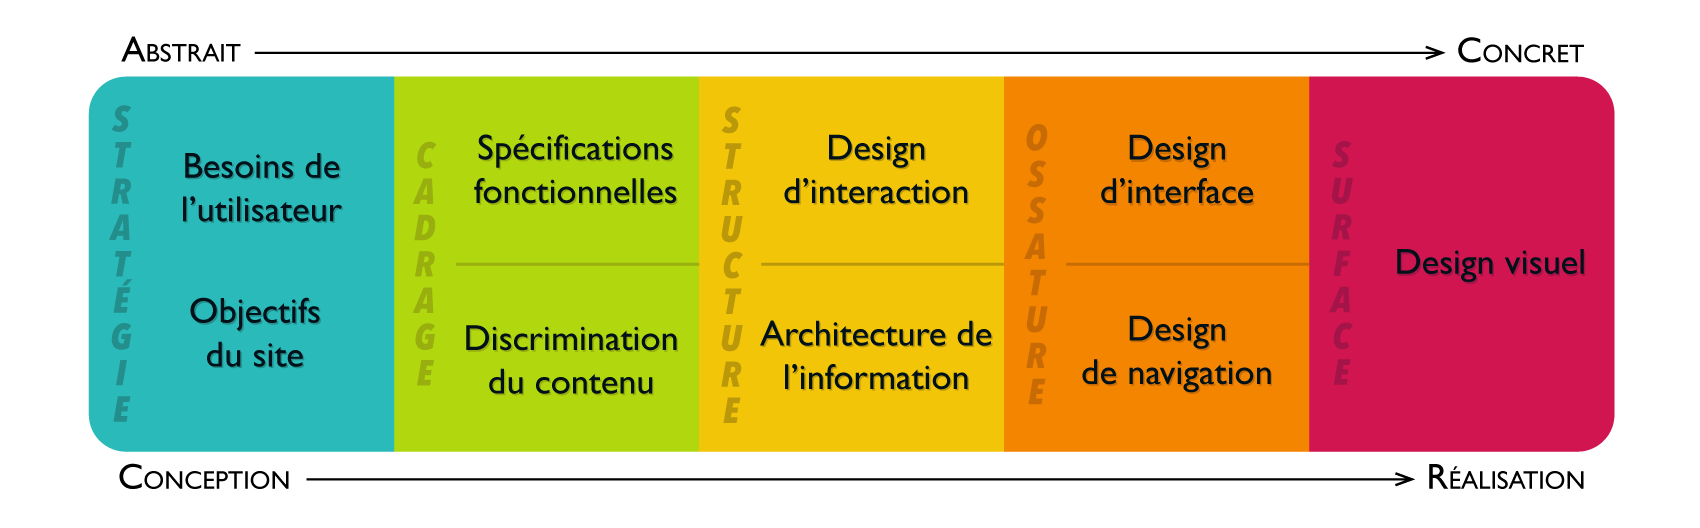
\includegraphics[width=14cm]{Images/Etape-UX-design.png}
	\caption{Schéma inspiré du diagramme de l'\ux conçu par J.J. Garrett}
\end{figure}

Le modèle de Garett\footnote{\cite{garrettAdditionalResources}} propose une élaboration en cinq étapes, correspondant à cinq niveaux de conception de l'interface, allant du plus abstrait au plus concret. Il s'agit tout d'abord de définir les enjeux et de circonscrire les besoins, en explicitant en quoi la construction de la plateforme est profitable. La deuxième étape de cadrage délimite le périmètre technique du projet, par l'établissement notamment d'un cahier des charges fonctionnel\footnote{Voir le tableau récapitulatif des interfaces à développer à l'annexe \ref{CahierDesCharges}.}. L'étape suivante concerne la structure globale de la plateforme~; y sont définis les scénarios de navigation et les interactions entre les différentes parties du site. La réflexion porte ensuite sur l'agencement de l'interface à l'intérieur de l'écran~: la composition générale et la cohérence structurelle des pages sont alors établies. Enfin, une dernière étape vient fixer la charte graphique de l'ensemble, dans le but de caractériser l'identité visuelle de la plateforme. Chacune de ces étapes sert de socle à celle qui suit. En effet, si l'apparence du site est la composante la plus remarquée de l'\ux par l'utilisateur, chacun des choix visuels se doit d'être justifié par les décisions structurelles précédentes.

Datant des années 2000, la méthode développée par J.J. Garrett nécessite quelques ajustements, mais elle reste pertinente pour guider le processus d'élaboration d'une plateforme dans ses grandes lignes. L'attention portée à chaque étape de la conception permet d'éviter des écueils qui pourraient causer le délaissement de la plateforme par son public.

		\subsection{Constitution d'un parcours de navigation}
			\subsubsection{Modalités de circulation dans l'interface}
Le parcours navigation s'inscrit dans les réflexions liées à l'architecture de l'information~: sa définition constitue une étape structurelle importante, qui détermine comment l'utilisateur va se repérer au sein de la plateforme. Plusieurs modèles de navigation peuvent être utilisés à l'intérieur d'une application Web.

\begin{figure}[h!]
	\centering
	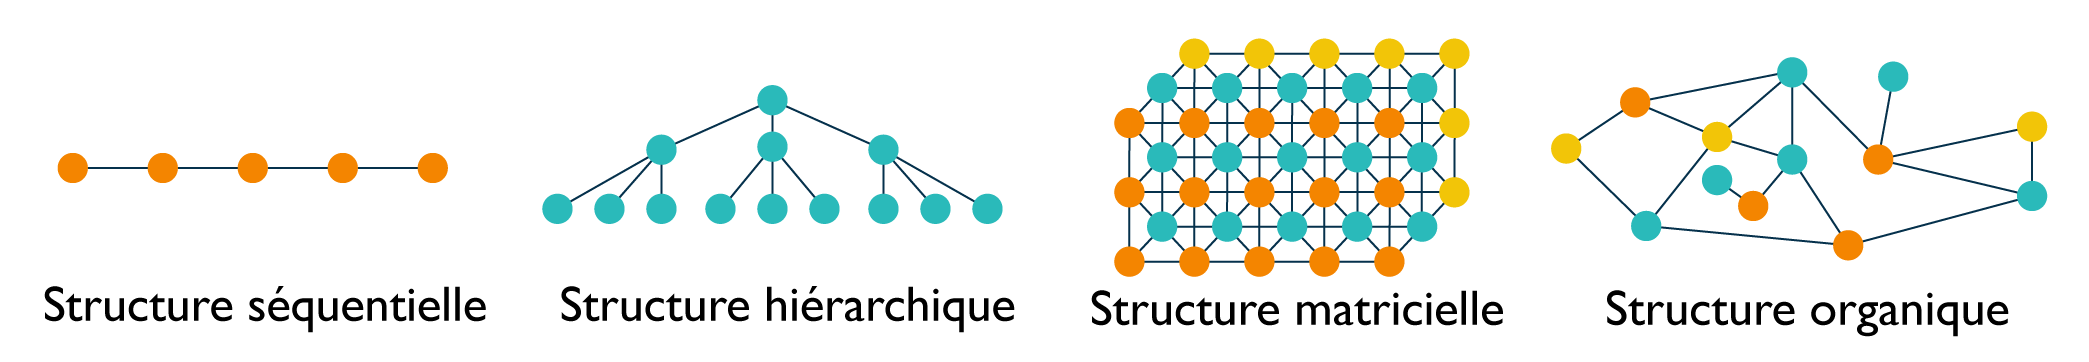
\includegraphics[width=15cm]{Images/Structure-navigation.png}
	\caption{Schéma inspiré du livre \emph{The Elements of User Experience}}
\end{figure}

La navigation séquentielle repose sur le déploiement successif des pages~: elle se rapproche de la logique linéaire du livre-codex.  On l'utilise généralement lorsque l'ordre de déroulement est essentiel, comme c'est le cas pour un tutoriel. La structure hiérarchique correspond à une formation en arborescence des pages~: ce type de structure, s'appuyant sur des relations parent-enfant, est bien compris par les utilisateurs, puisque c'est l'architecture utilisée pour l'organisation des fichiers informatiques. La structure matricielle superpose plusieurs plans, entre lesquels l'internaute peut se déplacer. Elle est utile lorsque les utilisateurs ont des besoins divergents, mais que les allers-retours doivent être possibles entre les différentes couches du site. La navigation organique ou hypertextuelle enfin, est la plus spécifique des modes de circulation du Web. Elle est plus intuitive, dans la mesure où elle suit le désir de l'utilisateur, mais induit un accès davantage discontinu à l'information. Cette structuration ne se fonde pas sur un modèle défini et donne ainsi l'impression d'une navigation libre dans les contenus, toutefois, elle rend aussi plus difficile de s'y repérer.

Ces structures entraînent différents rapports à l'information : leurs usages peuvent être combinés afin de laisser plus de liberté à l'internaute. La navigation influence profondément la compréhension du contenu~; elle est un mode d'expression du corpus, mais n'use pas des mêmes canaux que les supports plus classiques de l'exposition du travail scientifique\footnote{\g{Les dispositifs électroniques élaborés par les historiens sont puissamment structurés par les imaginaires de leurs créateurs et en particulier par les métaphores dont ils usent lorsqu’ils tentent de se les approprier. }\cite[§~14]{rygielOrdinateurReseauEcriture2006}}. Pour la médiation des données de recherche, il faut donc repenser entièrement les modalités de présentation et d'exploration.

			\subsubsection{Structure du \eng{front office}}
Ainsi, un choix éditorial doit être effectué pour la constitution du \eng{front office}~: il résulte entre autres, de la restructuration de l'information numérique. De manière à décrire précisément les sources, le modèle conceptuel de \dishas (figure \ref{Modelisation}) admet une grande complexité, mais un tel raffinement constitue un frein à la compréhension. En effet, la distinction entre contenu tabulaire (\eng{Table content}) et texte édité (\eng{Edited text}) n'a, par exemple, pas de sens dans une perspective explicative. Ainsi, certaines simplifications par rapport à l'interface administrateur ont été opérées pour définir la structure de la plateforme publique~; en particulier, le retrait des pages de notices\footnote{L'expression \g{pages de notice} est utilisée ici pour désigner les pages qui concernent un unique enregistrement dans la \bdd~: par exemple, une page qui présente un manuscrit en particulier.} d'entités secondaires. Les données relatives à ces tables –~comme par exemple celle des \eng{Historical actors}~–  ne sont pas supprimées des interfaces, mais considérées comme des métadonnées des entités principales.

Deux grands axes de navigation ont ensuite été déterminés, correspondant à la bipartition présente dans le modèle de données. La polarisation des parcours dans l'interface publique a été l'occasion de penser deux voies d'accès à la donnée~: une davantage historique, tournée vers les sources anciennes de l'astronomie~; et une autre orientée vers les aspects \g{scientifiques} du corpus, à savoir les éditions de tables et les paramètres astronomiques. Chacune de ces voies mène \eng{in fine} à l'entité centrale de la \bdd, à savoir la table astronomique. Ces deux parcours composent en ce sens, deux matrices parallèles qui se font écho à travers de multiples correspondances~: l'utilisateur, en fonction de ce qu'il cherche –~un manuscrit ou un paramètre~– sera dirigé vers l'une ou l'autre partie du \eng{front office}. Néanmoins, de nombreuses passerelles permettront de rebondir d'un côté à l'autre, assurant ainsi le décloisonnement de l'information.

\begin{figure}[h!]
	\centering
	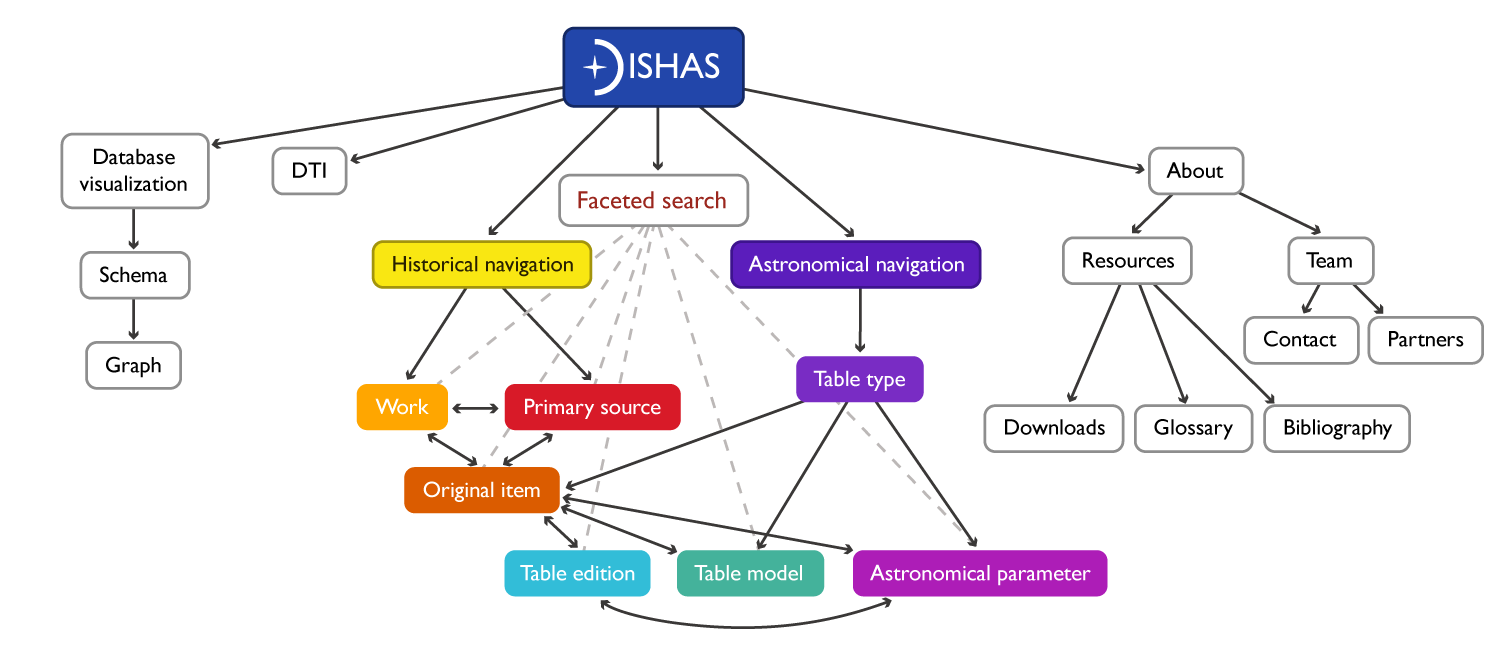
\includegraphics[width=17cm]{Images/Plan-frontoffice.png}
	\caption{Diagramme d'architecture de l'interface publique}
\end{figure}

L'abondante présence de liens est le support de l'interconnexion entre les ressources de l'interface~: par les redirections, il est possible de constituer un réseau sous-jacent qui se fait l'écho aux relations modélisées dans la \bdd. La navigation se construit ainsi de manière individuelle, chaque utilisateur dessinant sa propre séquence d'interactions\footnote{\g{Il s’agit, en d’autres termes, de créer des liens entre des textes et d’autres types de documents pour pouvoir organiser de façon dynamique nos parcours de lecture et de recherche et donc notre accès aux contenus.} \cite[§~6]{sinatraChapitreHistoireHumanites2014}}. Toutefois, une structure plus hiérarchique de l'information est maintenue, pour garantir un cadre dans lequel l'utilisateur peut de repérer.

Une organisation selon le niveau de granularité de la donnée permet ainsi de conserver une cohérence dans les contenus, en les ordonnant du plus général au plus spécifique. Dans cette logique, les pages de listes agrégeant les données conduisent aux notices d'enregistrement unique. De la même façon, les entités de nature mixte amènent vers les entités qui les composent~: pour accéder à un \oi, l'utilisateur devra donc transiter par la notice d'une source primaire ou d'une œuvre, dans la mesure où elles constituent un assemblage de tables. En dernier lieu, les fonctionnalités de recherche amènent un autre mode de navigation, celui de l'accès direct à la ressource à l'opposé de la libre circulation dans les interfaces. Enfin, des pages annexes (en gris sur le schéma) apportent en parallèle des contenus additionnels, utiles à la compréhension du projet de recherche.\\

Ainsi, ce plan permet à la plateforme publique de développer de nombreuses ramifications, tout en conservant une ossature relativement simple à comprendre. À chaque nœud de l'arborescence, il est possible de se déplacer en profondeur comme par translation, le but étant d'amener l'utilisateur le plus rapidement vers ce qu'il cherche. Le parcours de navigation pourra ainsi donner à l'internaute un accès local autant que des perspectives de longue portée sur la donnée. Chaque élément de la base y est replacé dans son environnement. Le \eng{front office} compose ainsi un discours sur la \bdd, un discours qui met au centre la table astronomique tout en mettant en valeur les données qui y sont corrélées.\\

Les chapitres suivants portent sur les différentes médiations de données qui ont été élaborées et conçues dans le cadre de mon stage~: certaines précisions doivent être énoncées avant de présenter mes réflexions et réalisations. Les différentes interfaces et visualisations réalisées ont fait l'objet de discussion avec l'équipe de recherche~; toutefois, le développement du \fo n'ayant pas été achevé, les interfaces conçues n'ont pas pu bénéficier de véritable retour d'expérience. De plus, la base sur laquelle s'appuient les visualisations accomplies est une \bdd de test, ne présentant ni l'exactitude, ni les dimensions de la base de données finale. Du reste, la durée de mon stage ne m'ayant permis de ne travailler que sur la navigation historique, l'accent sera donc mis sur l'élaboration des interfaces de cette partie. Le travail d'élaboration des interfaces, notamment pour le parcours astronomique, n'a pas été achevé~; les solutions présentées au sein de ce mémoire sont donc sujettes à modifications.

\clearemptydoublepage

\chapter[Médiation pour les publics non-spécialistes]{Présentation de la structure de données~: médiation pour les publics non-spécialistes}
En tant que vitrine, la plateforme publique de \dishas a pour vocation de présenter les missions de recherche du projet. Un utilisateur se rendant pour la première fois sur le site doit pouvoir identifier les ambitions scientifiques portées par \dishas, ainsi que les données exposées sur la plateforme. Plus encore que la donnée individuelle, c'est l'ensemble du modèle conceptuel qui doit être rendu explicite à l'internaute pour l'aider à comprendre la nature des ressources. En ce sens, la mission du \fo est de rendre les contenus accessibles intellectuellement à un public profane, en proposant une mise en forme éclairante de l'information.

	\section{Garantir l'ouverture à des publics non-spécialistes}
		\subsection{Organisation de l'information comme vecteur de compréhension}
L'architecture de la plateforme est l'un des véhicules de la clarification du propos scientifique\footnote{\g{la vulgarisation se pense à différents niveaux~: au niveau de l’écriture \p, dans le choix des sujets, dans la construction du texte, dans le fait de travailler avec un public précis en tête} \cite{hegaratApprendreVulgariser}}~; l'effort de médiation doit donc se porter à y faire transparaître l'organisation du corpus de recherche. La structure conceptuelle qui accueille le matériel documentaire doit être le support de la navigation~; elle participe à la compréhension de la nature des sources comme des enjeux scientifiques. En distinguant deux parcours vers la donnée, la plateforme offre deux points de vue sur le corpus. Ces deux parcours se calquent sur le modèle de données\footnote{Voir figure \ref{Modelisation}.}, lui-même traduisant le travail des chercheurs sur les ressources.

Dans le \fo de \dishas, deux modes de médiation du modèle conceptuel ont été explorés dans le parcours de navigation. Une organisation hiérarchique suivant les relations d'inclusion entre les différentes entités de la base et une organisation hypertextuelle traduisant les corrélations entre les éléments de l'architecture.

			\subsubsection{Structuration hiérarchique}
Contrairement aux bases orientées document, les liens hiérarchiques à l'intérieur d'une \bdd relationnelle ne sont pas directement apparents. Ce sont les cardinalités qui traduisent les formes d'inclusions entres les entités~; ce type de connexion entre les données, simple d'appréhension pour l'utilisateur, est important à rendre visible dans l'interface. Structurer les pages de la plateforme en reproduisant ces relations entre entités permet d'accompagner l'utilisateur dans sa compréhension du site.

La tripartition conceptuelle du document manuscrit –~production intellectuelle, témoin matériel, et élément tabulaire~– peut par exemple constituer une difficulté initiale pour le public. Toutefois, dans la \bdd, il est possible de voir qu'un \oi n'est toujours relié qu'à une œuvre et à une source primaire~; en ce sens, ces entités peuvent être considérées comme des \g{parents} de l'\oi. En effet, une œuvre comme une source primaire rassemble plusieurs tables~; en présentant l'\oi dans un second temps de la navigation –~toujours par le biais de la page de notice de son \g{parent}~– l'utilisateur est plus à même de saisir l'interaction entre ces trois entités.

De la même manière, il est possible d'architecturer l'information au sein d'une même page. Ainsi, la page de navigation astronomique se déplie à partir de l'entité centrale de l'objet astronomique. Le concept d'objet astronomique –~Lune, Soleil, Saturne, etc.~– est relié dans la \bdd avec de nombreuses entités, qu'il est possible de classifier en fonction du corps céleste auquel elles font référence. Chaque type de table\footnote{L'entité \eng{Table type} fait référence à la fonction d'une table, par exemple, le calcul de la vélocité solaire est un type de table.} est ainsi lié à un objet astronomique, chaque édition, set de paramètres\footnote{Un paramètre astronomique correspond à une valeur numérique signifiante au sein d'une table~: Voir \ref{Parametre}.} et modèle\footnote{Un modèle de table est la définition grâce à une syntaxe mathématique moderne de la fonction sous-jacente à une table~: Voir \ref{FormulaDefinition}.} étant eux-mêmes liés à un type de table. La conception de la page \eng{Astronomical navigation} s'est développée autour de cette structure~; l'objet astronomique y sert de point d'accès aux autres entités de la base.

			\subsubsection{Réseau hypertexte\label{Reseau-hypertexte}}
La manière hiérarchique de dérouler l'information permet d'ordonner les entités de manière à les rendre plus signifiantes. Néanmoins, l'exploration libre des contenus peut aussi aider l'utilisateur à faire l'expérience des corrélations entre les données~: en rebondissant de page en page, l'internaute tisse un réseau d'interactions. Chaque page de la navigation a donc été conçue comme un point névralgique, duquel rayonne une multiplicité de liens menant vers les contenus connexes. Ainsi, chaque élément de l'interface a été conçu pour être cliquable et rediriger vers l'entité à laquelle il fait référence. Les visualisations de données en particulier, illustrant le rapport entre les ressources, sont élaborées pour servir de portails~: chaque composant graphique constitue un lien sur lequel l'utilisateur peut cliquer, afin d'explorer davantage l'entité qu'il représente\footnote{Par exemple, sur un diagramme en colonne représentant les sources primaires contenant une œuvre, le clic sur une colonne occasionne la redirection vers la notice de la source primaire concernée.}.

L'objectif de l'interface est de retrouver la cohérence d'une donnée profondément éclatée par sa numérisation~: chaque page de notice doit composer une représentation intelligible du matériel documentaire de départ, ne se résumant pas à une simple collection de métadonnées. Avec l'aide des liens et des visualisations de données, l'interface publique doit traduire un enregistrement de la base en une représentation digitale du matériel documentaire.

		\subsection{Nécessité du contenu éditorialisé}
			\subsubsection{Création de contenu décrivant la donnée}
Cependant, la donnée ne se suffit pas forcément à elle-même pour être explicite. Afin de rendre les ressources de l'interface publique intelligibles, il faut parfois recourir à l'ajout de contenus explicatifs. Ces contenus peuvent avoir vocation à enrichir la donnée, à resituer son contexte de création, à la replacer dans une perspective de recherche scientifique ou encore simplement à la définir au sein du modèle de données.

Le contenu explicatif et la donnée fonctionnent de manière complémentaire et vise à fournir un accès optimal à l'information~: l'exemple de Wikipédia et Wikidata est en ce sens révélateur. Selon ses besoins, l'utilisateur utilisera l'une ou l'autre de ces plateformes pour accéder à ce qu'il souhaite. S'il cherche à se renseigner sur un sujet, il privilégiera l'encyclopédie en ligne~; s'il désire en revanche extraire des données pour leur appliquer un traitement, il préférera la base de Wikidata. La donnée brute est utile dans un cadre informatique, mais en termes de compréhension, les contenus éditorialisés sont préférables. Plusieurs types de textes explicatifs ont été intégrés à l'interface utilisateur de \dishas.

En premier lieu, il est évidemment essentiel à toute plateforme publique de recherche de disposer d'un texte introduisant les problématiques soulevées par son projet scientifique. Plusieurs versions de ce texte peuvent être composées~: pour \dishas, un texte court sur la page d'accueil sert de présentation~; tandis qu'une page \g{À propos} développe quant à elle une version étendue. Non moins primordiales, les définitions des différentes entités de la base doivent être rendues accessibles. Elles ont été dupliquées dans \dishas, à la fois au sein la page de chaque notice, mais également rassemblées à l'intérieur d'un glossaire. D'autres textes introductifs sont destinés à intégrer la plateforme~; lors de la conception des interfaces, il a semblé à plusieurs endroits nécessaires l'adjonction de contenus explicatifs. Dans l'attente de leur rédaction par l'équipe de recherche, des espaces ont été aménagés lors du développement des vues à l'aide de texte de remplissage.

En effet, la création de contenus éditorialisés est le fruit d'une collaboration entre chercheurs et ingénieur~; l'ingénieur aidant à identifier quelles productions scientifiques contribuent à une meilleure médiation, et le chercheur contrôlant par son expertise scientifique la pertinence des interfaces. En outre, si l'application Web de \dishas n'a pas pour mission d'être une plateforme de publication des productions des chercheurs, une sélection de ressources diverses peut être mise à disposition de l'internaute s'il souhaite approfondir sa connaissance en astronomie ancienne. Cette documentation pourra se composer d'une bibliographie, de diapositives présentées lors de séminaires, de liens vers des ressources en ligne, etc.

L'ensemble de ces contenus façonne un contexte dans lequel la métadonnée informatisée trouve son sens. Cette éditorialisation de l'interface peut être distillée au sein des pages de visualisation de données –~grâce aux définitions et textes introductifs~– mais également dans les pages périphériques à la navigation, où peut être centralisée la documentation utile à un internaute curieux souhaitant pousser son exploration.

			\subsubsection{Donner à voir par la visualisation}
L'éditorialisation du corpus peut cependant s'exprimer par de multiples canaux\footnote{\g{L’édition se transforme en éditorialisation : l’ensemble des pratiques d’organisation et de structuration de contenus sur le web. La différence principale entre le concept d’édition et celui d’éditorialisation est que ce dernier met l’accent sur les dispositifs technologiques qui déterminent le contexte et l’accessibilité d’un contenu, ainsi que sur la réflexion autour de ces dispositifs.} \cite[§~20]{sinatraChapitreHistoireHumanites2014}}. La conception de visualisations de données permet de repenser l'accès au contenu~; en effet, les visualisations expriment par un vocabulaire graphique ce qu'il est parfois plus difficile à retranscrire à l'écrit. Elles constituent en ce sens un vecteur privilégié pour la médiation.

Les visualisations de données véhiculent dans leurs représentations des informations vis-à-vis du contenu. Un diagramme ne produira pas les mêmes évocations auprès du public selon qu'il soit linéaire, en barres ou en colonnes. Afin de trouver la meilleure représentation visuelle de la donnée, il est important de considérer les idées sous-tendues derrière chacune d'elles. Lors des réflexions liées à la création de la page de notice pour les œuvres, plusieurs formats ont été expérimentés pour représenter le lien entre œuvre, source primaire et \oi.

\begin{figure}[H]
	\centering
	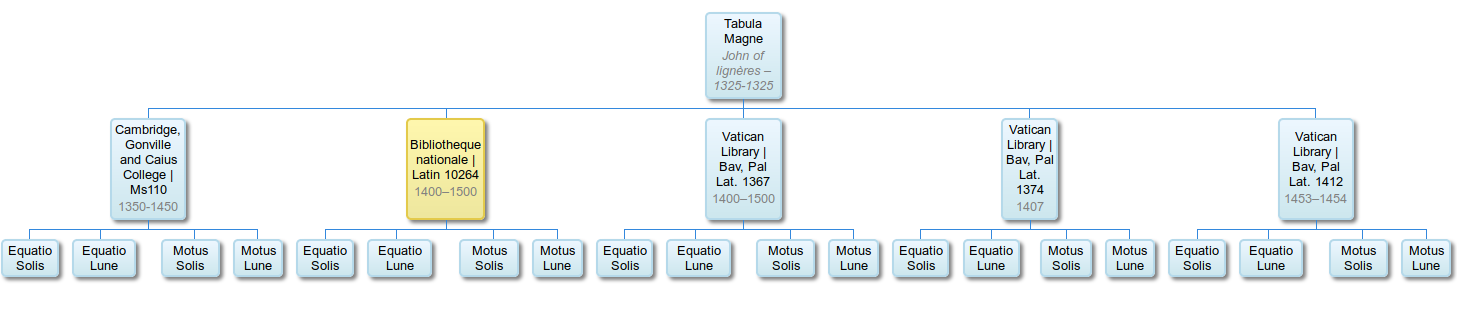
\includegraphics[width=16cm]{Images/Visualisations/Premiers-essais/Work-organigramme.png}
	\caption{Organigramme réalisé avec \eng{Google charts} lors de phase d'élaboration des interfaces\label{Organigramme}}
\end{figure}

Par exemple, la représentation sous forme d'organigrame (cf Figure \ref{Organigramme}) d'une œuvre pose plusieurs problèmes~: en premier lieu, la disposition horizontale de la visualisation est susceptible d'excéder rapidement la largeur d'un écran, si le jeu de données est trop important. En outre, l'organigramme est un type de visualisation qui évoque une hiérarchie entre les éléments, alors que le modèle de données établit l'œuvre et la source primaire comme étant deux versants de l'\oi. Si l'œuvre préexiste au manuscrit, elle n'en est pas la parente. Ainsi, la visualisation, bien que juste, véhicule de fausses impressions sur la donnée et n'aide pas l'utilisateur dans sa compréhension des sources.

\begin{figure}[H]
	\centering
	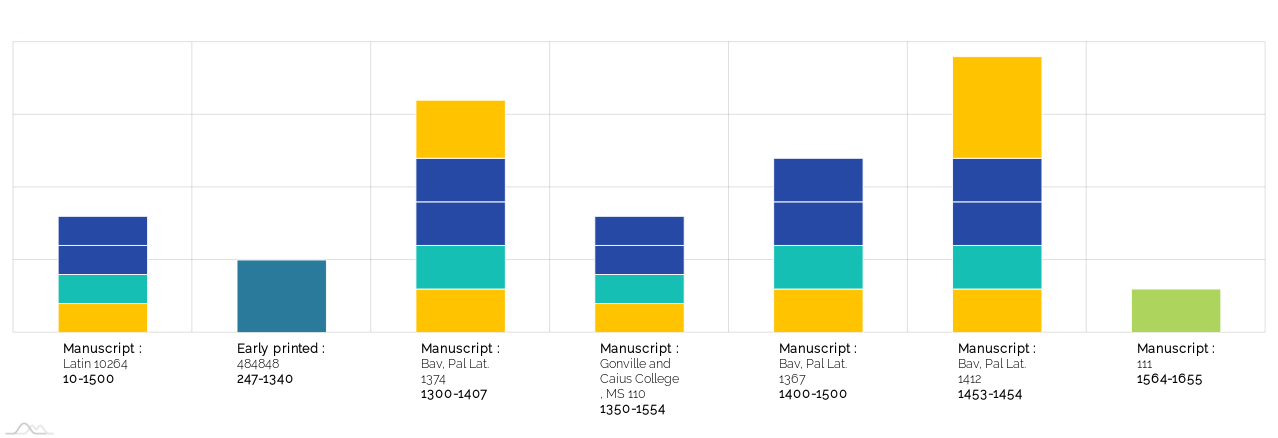
\includegraphics[width=16cm]{Images/Visualisations/Work-Tabule_Magne.png}
	\caption{Diagramme en colonnes conçu avec \eng{AmCharts} pour les notices d'œuvres}
\end{figure}

La visualisation élaborée pour la page de notice d'une œuvre évite les écueils de l'organigramme. Ici, chaque colonne correspond à une source primaire contenant l'œuvre de la \emph{Tabule Magne}. Chacune de ces colonnes est composée de blocs, représentant chacun un \oi contenu dans la source primaire. La hauteur des blocs est proportionnelle au nombre de folios de l'\oi en question, la couleur faisant référence à l'objet astronomique dont il traite. Ainsi, d'un seul coup d'oeil, l'utilisateur peut repérer la complétude de l'œuvre dans chacune des sources primaires, pour se faire une idée générale de leurs contenus. En peu d'espace, de nombreuses informations sont transmises à l'utilisateur, et la relation entre les données est rendue visible sans être dénaturée.

	\section{Attractivité des contenus}
L'usage du numérique permet de concevoir de nouvelles médiations en regard de celles employées pour le format imprimé\footnote{\g{Nous trouvons trace également de dispositifs savants nouveaux, sans équivalents papiers \p.} \cite[§~8]{rygielOrdinateurReseauEcriture2006}}~: les modes de présentation de l'information doivent être repensés pour prendre en compte la plus vaste diffusion des ressources permise par l'informatique. Afin de susciter l'intérêt du public, la seule mise à disposition du contenu n'est généralement pas suffisante. Si l'architecture de l'information aide à le rendre cohérent, sa mise en forme graphique participe à son attractivité~: en effet, le succès d'une plateforme est en partie occasionné par le soin apporté à ses visuels. Plusieurs éléments sont à prendre en compte dans la création d'une plateforme~: l'aspect graphique bien sûr\footnote{\g{La création artistique et tout particulièrement le design numérique (art appliqué au numérique), est sans conteste un acteur clé de ce renouveau scientifique.} \cite{massotDessinerActeursHumanites2018}}, mais également l'intuitivité et l'interactivité des interfaces, qui impliquent l'internaute dans sa navigation.

		\subsection{Cohérence des interfaces}
				\subsubsection{Définition d'une charte graphique}
La définition d'une charte graphique pour la plateforme publique de \dishas vise deux objectifs~: rendre les interfaces plus attractives visuellement, mais également assurer la cohérence entre les pages. La navigation hypertextuelle a tendance à rendre le propos décousu~; la reprise d'éléments graphiques le long du parcours de l'utilisateur peut être utile à l'intelligibilité du discours. L'enveloppe visuelle de la plateforme ajoute une couche de signification au contenu, en mettant en avant les informations principales et en tissant des liens entre les composants de même nature. En repérant clairement les entités de la base à l'aide de couleurs et de pictogrammes distincts, il est possible de rendre le modèle de données plus apparent au travers de la plateforme. Par ailleurs, l'interaction entre les vues doit répondre à une logique unique, chaque élément devant réagir de la manière la plus adéquate aux attentes de l'utilisateur\footnote{Le principe d'adéquation de l'apparence et du comportement dans le domaine du design est nommé par Donald Norman \g{affordance}.}.

\begin{figure}[h!]
	\centering
	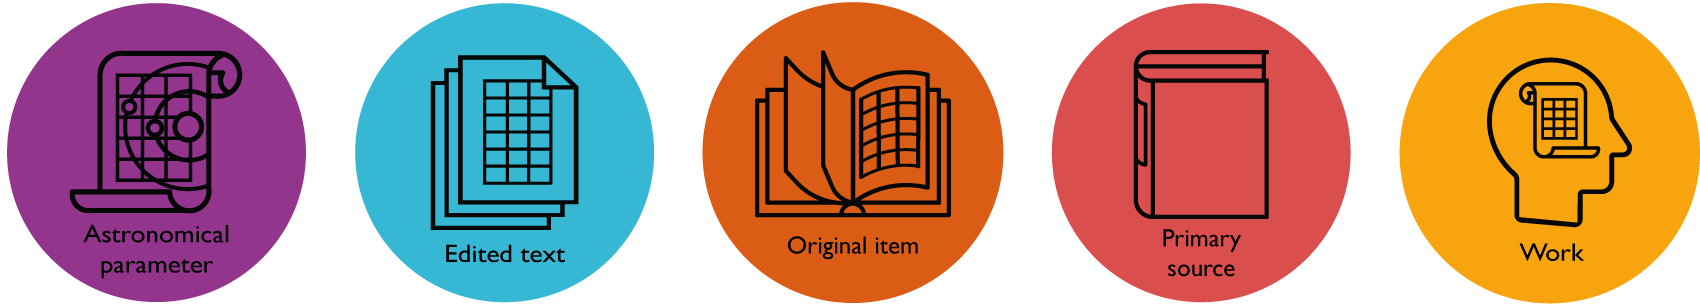
\includegraphics[width=10cm]{Images/Pictogrammes.png}
	\caption{Pictogrammes élaborés pour les principales entités de la plateforme de \dishas}
\end{figure}

L'identité visuelle des pages publiques a été élaborée en contraste de l'apparence du \eng{back office}. L'ensemble a été pensé pour être ludique et facile d'appréhension~: les visualisations de données ont par exemple été placées au centre des pages de notices. En outre, des pictogrammes pour chaque entité ont été conçus et utilisés comme des repères dans l'arborescence du site~; des couleurs leur ont été assignées pour renforcer encore l'impression de cohésion entre les parties du \fo. Enfin, le comportement des éléments a reçu un soin particulier, à l'instar du mouvement de déploiement et de repli de la barre latérale\footnote{Des captures d'écrans vidéos ont été prises des interfaces et ajoutées dans les fichiers annexes.} sur les pages de notices\footnote{Voir la fonction pour le comportement de la barre latérale à l'annexe \ref{sidebar-template}~: l'ouverture est déclenchée au clic sur un pictogramme et la fermeture au clic en dehors de la barre latérale.}, de manière à renforcer l'ergonomie de la plateforme.

			\subsubsection{Construction des pages de notice}
Toutes les pages de notices ont été conçues sur le même modèle~: en haut de l'écran, une aide à la navigation rappelle à quel endroit de l'arborescence se trouve l'utilisateur. En dessous de ce \g{fil d'Ariane}\footnote{Pour plus d'informations concernant la réalisation des \eng{breadcrumbs}, voir à l'annexe \ref{bread-crumbs}.}, un titre offre des renseignements quant à l'entité en train d'être visualisée, et introduit la visualisation graphique qui occupe l'essentiel de l'espace, chaque entité disposant d'une visualisation différente. Enfin, sur la gauche, une barre latérale peut être déployée afin d'afficher à l'écran les métadonnées relatives au présent enregistrement, mais aussi d'en donner une définition ou encore de proposer des exports des informations contenues dans la page.

\begin{figure}[h!]
	\centering
	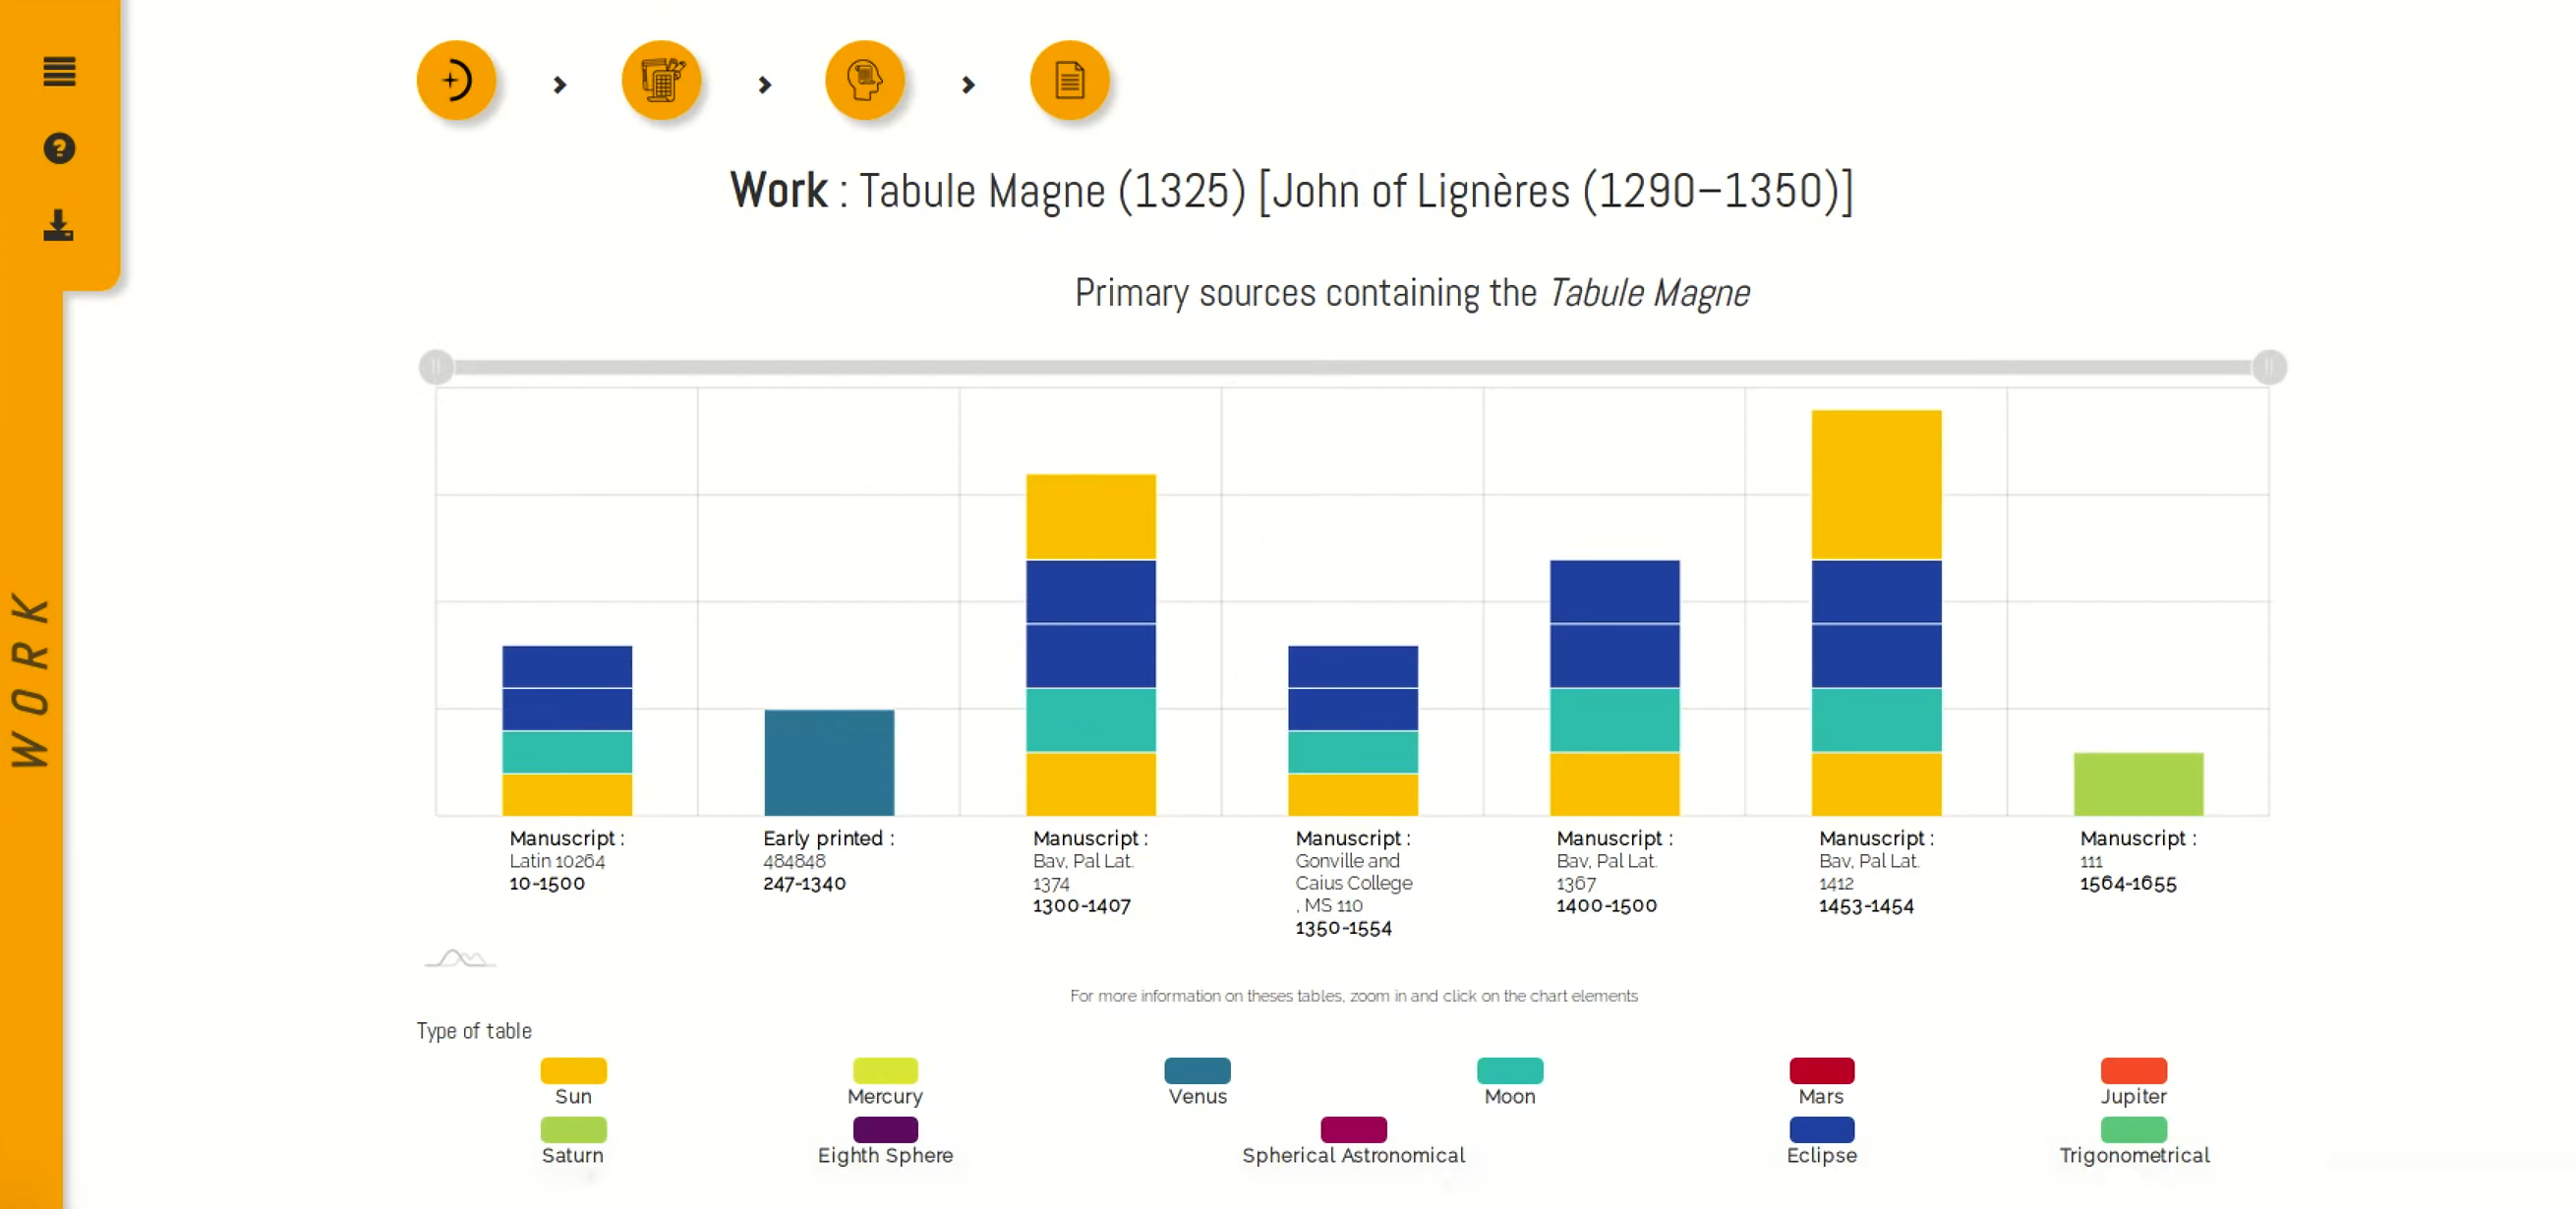
\includegraphics[width=15cm]{Images/Template-record-page.png}
	\caption{Exemple de page de notice pour l'œuvre de la \emph{Tabule Magne}}
\end{figure}

De manière à enrichir les notices, chacune des pages agrège les informations relatives aux entités connexes à un enregistrement. En croisant les données des différentes tables de la base, l'interface compose de nouvelles métadonnées pour l'entité à visualiser. De cette façon, l'utilisateur n'a pas seulement accès aux métadonnées d'un unique enregistrement~: il lui est aussi par exemple possible de connaître les langues présentes dans un manuscrit, alors que la table \eng{Language} n'est reliée qu'à la table \Oi\footnote{Il s'agit en effet de métadonnées de métadonnées au sein de la base.}. Le choix des métadonnées à afficher dans une notice doit être l'objet de considération, certaines données n'étant pas pertinentes à faire figurer~: par exemple, il serait trompeur d'indiquer une liste de bibliothèques à l'intérieur d'une notice d'œuvre, l'œuvre étant un concept intellectuel, plutôt qu'un objet susceptible d'être conservé.

Enfin, il est possible d'inscrire les notices de \dishas dans une structure plus large que la simple \bdd du projet. Dans la phase de modélisation, le recours à des normes permet d'ouvrir les silos informationnels~; lors de la conception d'interfaces, la redirection vers les notices connexes des plateformes en ligne de ces normes aide au décloisonnement de l'application Web. Les notices de tables astronomiques, bien que ne répondant pas aux modèles de description bibliographique classiques, peuvent ainsi s'ancrer dans un écosystème de ressources numériques~; les pages d'enregistrement de \dishas pourront ainsi à l'avenir être référencées en retour par les institutions de conservation, de manière à enrichir les notices de leurs collections en ligne.

		\subsection{Intégration de modules interactifs}
			\subsubsection{Implication de l'internaute}
L'exemple des expositions en ligne nous renseigne sur les différences entre exhibition matérielle –~davantage linéaire et dirigée~– et virtuelle des sources –~transversale et interactive. Le cas de l'exposition \g{Le monde en sphères}\footnote{\g{Le monde en sphères} Bibliothèque nationale de France (16 avril - 21 juillet 2019). Commissaires d'exposition~: Catherine Hofmann \& François Nawrocki.} est significatif, puisque les ressources exposées comprenaient de nombreux objets, notamment des globes, dont la corporéité pose la question de la numérisation. La modélisation 3D des globes a été choisie pour remplacer le dispositif en vitrine, laissant l'utilisateur libre de la manipulation pour le choix de l'angle de vue le plus adéquat\footnote{Des écrans tactiles permettant aux visiteurs de manipuler les globes dans leur version 3D ont été intégrés au parcours d'exposition de la \textsc{b}n\textsc{f}.}. Cette forme de médiation aide donc l'internaute à s'emparer des ressources digitales, sans occasionner de perte notable vis-à-vis du document original. La présentation numérique d'un corpus implique donc d'adapter les méthodes d'appréhension des sources~: si la dématérialisation des documents implique une distanciation et une restriction\footnote{\emph{Cf}. \g{Les numérisations de documents originaux} \cite{bertrandHistorienMedievistePratique2007}}, l'implication de l'utilisateur à leur exploration permet une réappropriation du contenu.

Les visualisations de données statiques véhiculent l'information de manière unilatérale~: l'ajout d'interactivité aux interfaces permet de laisser l'utilisateur manipuler la donnée pour lui donner la forme qu'il trouve la plus signifiante\footnote{\g{\eng{For web applications, on the other hand, the shape and form of live data coming from some data source are not always known upfront. So, whatever you imagine about the data in the design phase may turn out slightly or majorly wrong in production. Even in the least extreme cases, the chart type you chose to visualize the data may not be the best one from viewers perspective considering both the data itself and the insights they are trying to gain from it.}} \cite{LetViewersChange2018}}. La dimension dynamique d'une plateforme, tout en participant à son attractivité, propose à chaque utilisateur de façonner des visualisations sur mesure~; en ce sens, elle adapte le discours, sans simplifier le propos.

			\subsubsection{Visualisations de données modulables}
Plusieurs formes d'interactivité ont été intégrées aux contenus Web de la plateforme publique. La forme la plus élémentaire d'interaction avec le contenu graphique est le zoom. Chaque visualisation développée pour les interfaces dispose d'un système de zoom en conformité avec son type~: l'utilisation de la molette sur une carte entraînera son agrandissement, tandis que la sélection d'une zone sur une barre de déroulement (\eng{scrollbar}) occasionnera l'étalement horizontal du diagramme.

Par ailleurs, la visualisation élaborée pour la notice de source primaire dispose de deux états entre lesquels l'utilisateur peut alterner. Cette visualisation vise à synthétiser l'ensemble des \oi contenus dans la source, en les classant par œuvre. Un premier état représente tous les \oi de manière accumulée, tandis que dans le second état, les \oi sont répartis sur le graphique selon la même disposition qu'au sein de la source primaire. Si l'utilisateur veut estimer la portion de chaque œuvre dans un manuscrit, il préfèrera la première configuration~; s'il s'intéresse en revanche à l'aspect composite du document, la seconde configuration lui conviendra davantage\footnote{Pour une description plus précise de la visualisation, voir section \ref{Visualisation-PS}.}.

Enfin, une troisième forme de modularité a été ajoutée aux interfaces~: elle repose sur la mise en relation de plusieurs formes de représentations graphiques de l'information. L'assemblage de deux différents types de visualisations de données permet, grâce aux systèmes de sélection et zoom de chacun de ces types, de croiser et de raffiner les données à visualiser. Il est ainsi possible à l'utilisateur de n'afficher à l'écran que les ressources qui l'intéressent, confectionnant de cette manière une visualisation sur mesure. Son élaboration sera évoquée plus en détail dans la section \ref{HistoricalMap}.\\

La mission de présentation du projet \dishas par le \fo s'appuie donc avant tout sur une mise en forme attentive du contenu. L'architecture de l'information tout d'abord, guide l'internaute dans sa découverte du corpus de recherche, en s'enracinant sur le modèle de données. L'adjonction de contenus éditorialisés ensuite, fournit le socle explicatif sur lequel la donnée peut trouver son sens~; elle assure également une introduction scientifique de qualité au projet de recherche. Enfin, la définition graphique de l'interface, autant vis-à-vis de l'apparence de ses composants que du comportement de ses visualisations, achève de composer une plateforme ouverte à un public varié.  

\clearemptydoublepage

\chapter[Participation au travail de recherche]{Mise en valeur des données et de leurs interactions~: participation au travail de recherche}
Les chercheurs constituent la part la plus importante du public de la plateforme publique de \dishas~: importante en termes de nombre, mais également du point de vue de leurs attentes. La constitution du corpus de \dishas permet aux chercheurs de travailler sur des ensembles de sources considérables~; il est du rôle de la plateforme en ligne d'aider à embrasser plus facilement leur diversité. En fournissant des outils pour examiner la donnée dans ce qu'elle a de spécifique, ainsi que des instruments pour illustrer des assemblages importants de ressources, les chercheurs peuvent combiner des méthodes de \eng{close} et \eng{distant reading}\footnote{\g{\eng{Close reading is the thorough interpretation of a text passage by the determination of central themes and the analysis of their development.}} / \g{\eng{[Distant reading] aims to generate an abstract view by shifting from observing textual content to visualizing global features of a single or of multiple text(s).}} \cite{janickeCloseDistantReading2015}} dans leur analyse du corpus.

La construction du \fo est l'occasion de créer des médiums nouveaux pour l'exploitation scientifique des sources\footnote{\g{En effet, l’arrivée d’Internet est un moment clé dans le développement des humanités numériques, car il n’est pas un simple outil supplémentaire pour la recherche : il devient aussi un objet de recherche et, finalement, une technique qui modifie l’ensemble de nos pratiques au-delà de la communauté savante et, plus généralement, notre façon de voir le monde.} \cite[§~11]{sinatraChapitreHistoireHumanites2014}}. Le travail de création des interfaces s'est ainsi concentré sur l'élaboration de visualisations signifiantes ainsi que d'interfaces sur mesure pour l'accueil de la donnée.

	\section{Décloisonnement des corpus spécialisés}
		\subsection{Enrichir les données par l'interconnexion}
			\subsubsection{Connecter les ressources de la base de données}
L'analyse des sources numériques exige de rendre manifestes les interactions entre les données. En effet, un enregistrement isolé dans une base constitue difficilement une ressource suffisante à l'analyse~; c'est dans le réseau qui lie les différentes entrées de la base que se trouve le matériau sur lequel peut s'appuyer le travail scientifique. Le \fo doit révéler cette trame d'interconnexions, afin d'aider les chercheurs à reconstituer les liens entre des ressources éloignées. La réunion de tables de différentes traditions dans un même corpus doit être l'occasion de créer des interfaces riches, où il est possible à l'utilisateur de déceler par exemple les échanges intellectuels qui se sont opérés.

Le premier instrument de cette mise en connexion est l'interface de recherche. Afin de parcourir efficacement les collections, le \fo soit se dôter de fonctionnalités de recherche avancées, permettant au chercheur de filtrer parmi les ressources, pour réunir dans les résultats les données qui l'intéressent. La page de recherche de la plateforme publique ne dispose pas pour l'instant de système de filtres abouti~; la seule recherche plein-texte est disponible à l'utilisateur. Néanmoins, ce filtrage permet déjà d'effectuer des recherches assez précises. L'implémentation en outre du moteur de recherche ElasticSearch\footnote{Pour une présentation plus développée du fonctionnement d'ElasticSearch, voir chapitre \ref{Elastic}.} apporte différentes fonctionnalités qui renforcent l'efficacité de la recherche~: la \g{\eng{fuzziness}}, entre autres, autorise un certain degré d'imprécision quant à l'orthographe des termes. Cela permet par exemple, de retrouver un auteur même en utilisant une graphie différente de celle encodée dans la base. Par ailleurs, ElasticSearch permet d'exécuter des requêtes, non seulement sur les champs liés à une entrée du corpus numérique, mais également sur les champs des entités qui lui sont associés~: cela signifie qu'il est possible de retrouver tous les manuscrits contenant l'œuvre de la \emph{Tabule Magne}, alors que l'œuvre n'est liée qu'à un \oi dans le modèle de données.

Ces fonctionnalités extensives de recherche sont particulièrement utiles à l'identification de ressources connexes, car il a été observé que les utilisateurs sont parfois rétifs à l'utilisation de modalités avancées de recherche. En outre, l'utilisation de caractères génériques (\eng{wildcards}) et d'opérateurs booléens –~fonctionnalités prévues par ElasticSearch~– dans les termes de requêtes renforce encore l'acuité des résultats d'une simple recherche par mots-clefs.

			\subsubsection{\label{OuvrirMeta}Ouverture grâce aux métadonnées}
L'interconnexion des données a constitué un enjeu principal dans la construction des interfaces publiques. Il était important de reconstituer dans chacune des pages le réseau des données à l'intérieur de la base~: les pages de notices ont donc été élaborées comme des nœuds, desquels se propage une série de liens vers les entités apparentées. Comme il a déjà été mentionné\footnote{Voir la section \ref{Reseau-hypertexte}.}, les composants graphiques des visualisations permettent \eng{via} le clic de rediriger l'utilisateur vers les entités représentées~; mais la barre latérale de métadonnées a également fait l'objet d'aménagements particuliers pour réinscrire la donnée isolée dans son contexte relationnel. En premier lieu, grâce à l'enrichissement des notices par le croisement des données, mais également par la mise à disposition d'ouvertures relatives aux métadonnées d'un enregistrement. En effet, à côté de chacun des champs décrivant une notice, une icône de loupe a été placée~: elle donne accès aux entités de même type partageant la même métadonnée. Il est par exemple ainsi possible de retrouver toutes les œuvres conçues par un même auteur (par Jean de Lignières dans le cas de la \emph{Tabule Magne})~: en cliquant sur cette icône\footnote{Au survol, les termes de la requête exprimés en langage naturel apparaissent à l'écran~: par exemple, \g{Toutes les œuvres conçues par Jean de Lignières}.}, l'utilisateur est envoyé sur la page de recherche où les résultats de la requête correspondante apparaissent.

\begin{figure}[h!]
	\centering
	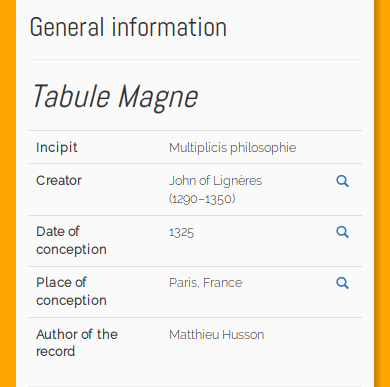
\includegraphics[width=9cm]{Images/Sidebar/metadata-work.png}
	\caption{Barre latérale des métadonnées de l'œuvre de la \emph{Tabule Magne}}
\end{figure} 

Ce mode de circulation dans les données permet d'anticiper les potentielles questions de recherche des utilisateurs~: l'ajout systématique de ces \g{loupes} aux métadonnées connecte la notice à tous les enregistrements partageant une même caractéristique. Les loupes permettent de décrire des ensembles cohérents dans les ressources de la base. Elles constituent une fonctionnalité alternative de recherche, correspondant en réalité à une forme de requête facettée\footnote{Le clic de l'utilisateur envoie à ElasticSearch une requête formulée préalablement dans le \eng{back end}, la page de recherche met ensuite en forme les résultats reçus. L'implémentation des fonctionnalités d'ElasticSearch dans \dishas est plus amplement discuté à la section \ref{Elastic}.}. Quelque soit l'angle d'approche du chercheur, cette voie d'accès à la donnée offre des perspectives pour élargir les corpus de recherche.

		\subsection{Constitution d'une interface spécialisée : le cas des éditions de tables}
Les éditions de tables sont un objet central de la \bdd de \dishas~; leur mise en valeur au sein de l'interface publique constitue l'un des enjeux cruciaux de la plateforme en ligne. En effet, les contenus tabulaires sont un matériau essentiel de la recherche en astronomie ancienne et le projet \dishas a été envisagé dès le départ comme un moyen de leur mise en commun. Si l'interface numérique offre des perspectives renouvellées pour l'édition critique, elle peut également dérouter lorsqu'elle n'est pas conçue correctement\footnote{\g{L'extraordinaire possibilité de faire des allers-retours entre document original numérisé et texte édité (qui décuple les possibilités de contrôle et d'appropriation de l'édition par le lecteur), de naviguer entre plusieurs pages (plus vite et plus pertinemment que dans le volume papier) \p arrive pourtant assez vite à saturation~; les actes, les sections de texte se trouvent largement coupés de leur contexte} \cite{bertrandHistorienMedievistePratique2007}}.

			\subsubsection{Problématiques de l'édition critique de tables}
Préalablement à la conception d'une interface, il est primordial d'identifier les problématiques spécifiques liées à l'édition de tables. Au premier chef, le format tabulaire impose de réfléchir à un moyen de repérer l'apparat critique~: la pratique des chercheurs varie sur ce point. Pour certaines éditions, la table est encadrée par deux axes numérotés permettant de désigner une case à l'aide de coordonnées~; d'autres distinguent chaque variante à l'aide d'un nombre\footnote{Cette méthode est la plus proche de la manière dont sont encodées les tables dans la base~; chaque variante est indiquée à l'endroit même de la case. La syntaxe est semblable à celle-ci~:\newline\texttt{[\{"valeur": 12, "apparat-critique": "Ms-1:11, Ms-2:13"\}]}.}, tandis que d'autres encore, dupliquent le cadre de la table pour n'y reproduire que les variantes. D'autres procédés existent pour baliser l'apparat critique~; ils disposent tous d'avantages comme d'inconvénients. Toutefois leur complexité rend parfois la lecture d'une édition critique particulièrement laborieuse\footnote{Selon les propos recueillis lors des séminaires organisés avec l'équipe de recherche de \dishas.}.

Une seconde difficulté est liée à la mise en page. Dans les manuscrits souvent, les tables sont accolées les unes aux autres sur la page, et parfois se poursuivent sur plusieurs folios à la fois. Il peut ainsi être ardu de transposer ces configurations à l'intérieur d'une édition, en particulier lorsque le format de la page impose ses bornes. Pour assister au travail d'édition, l'outil \dti offre de nombreuses fonctionnalités pour la saisie des tables\footnote{Voir la section \ref{DTI}.}, la plateforme doit quant à elle fournir une interface adaptée à la présentation de ces tables.

			\subsubsection{Propositions de fonctionnalités}
Afin d'aider les chercheurs à accéder aux sources, l'interface de visualisation d'une édition doit intégrer les questionnements liés à la publication imprimée~: un affichage ergonomique de l'information doit résulter de ces réflexions. Dans le but de pouvoir être éventuellement mentionnée au sein d'un article, la notice d'édition de table dans la plateforme publique a été particulièrement soignée~; son élaboration a fait l'objet de multiples discussions avec l'équipe de recherche. Cependant, la construction de l'interface n'a pas été entamée. Les solutions présentées ci-après feront l'objet de développements futurs, la mise en forme de l'interface est donc également susceptible d'être corrigée\footnote{La cahier des charges relatif à la réalisation des interfaces publiques donne des renseignements plus précis quant au développement de la notice d'édition~: voir en annexe \ref{CahierDesCharges}.}.

Dans le but de prendre en compte les différentes perspectives de recherche, la page de notice d'une édition doit se déployer sur quatre onglets~: historique, mathématique, éditorial et contenu tabulaire. Ces quatre onglets, dédiés à différents aspects de l'édition, pourront être chargés séparément afin d'optimiser les temps d'attente pour l'utilsateur. Le contenu tabulaire sera placé en position liminaire, de manière à être visualisé en premier.

L'onglet historique doit porter sur le contexte de production de la source primaire éditée~; il sera donc disponible uniquement pour les éditions de type \textsc{a} et \textsc{b}, dans la mesure ou les types \textsc{c} sont recalculés entièrement. Cet onglet comprendra les informations relatives à l'œuvre, la source primaire et l'\oi d'où provient l'édition. L'onglet mathématique concernera la tradition astronomique dans laquelle s'inscrit la table, en présentant les informations relatives aux paramètres utilisés en son sein. L'onglet éditorial présentera l'auteur et le contexte de publication, l'édition étant potentiellement tirée d'une version imprimée auparavant. Chacun de ces onglets comportera une visualisation de données différente, sous forme de carte pour les deux premiers, et sous forme de graphe pour le dernier.

L'onglet présentant le contenu tabulaire édité sera présenté sous forme de tableau de nombres. Dans le cas d'une édition critique (type \textsc{b}), un encart latéral permettra d'afficher l'apparat critique au clic sur une case~; il est possible d'imaginer un dispositif pour faire apparaître l'apparat critique de multiples cases simultanément. Un système d'intensité de couleur indiquera la densité des variantes pour les différentes cellules du tableau, identifiant ainsi les passages problématiques de la computation. Une autre sorte de repère visuel signalera la présence de commentaires. Enfin, un lien permettra d'ouvrir l'édition dans l'interface de saisie de table, afin de pouvoir la manipuler grâce aux outils implémentés dans \dti. Plusieurs détails de l'interface restent encore à préciser~: doit-on permettre à l'utilisateur de visualiser plusieurs tables de manière concomitante~? Quels formats d'export sont les plus adaptées à ce genre de contenu~? Comment concevoir la mise en page de tables à double argument~? Ou encore, comment afficher l'apparat critique à l’intérieur du panneau latéral~?\\ 

Le développement de cette interface occasionnera assurément d'importantes modifications par rapport à cette première ébauche~: la réalisation technique en effet devra être effectuée en collaboration étroite avec l'équipe de recherche. Les éditions de tables constituent la donnée pivot du projet \dishas~: la page de notice publique doit faire le lien entre sources historiques et paramètres astronomiques. Par la conception d'une interface sur mesure, les chercheurs disposeront d'un support adapté à la présentation et la consultation des tables éditées. Cette interface constituera en ce sens un atout du projet, pouvant inciter les chercheurs \emph{a posteriori} à ajouter davantage de données de manière à enrichir encore la plateforme en ligne.

	\section{Analyse par la visualisation}
Contrairement à l'infographie où sont organisées visuellement des données connues à l'avance, la visualisation de données dynamique s'appuie sur des données mouvantes, dont il n'est pas possible de prédire avec exactitude la manifestation graphique. En ce sens, la visualisation révèle des informations sur les ressources qu'elle représente, elle les ordonne de manière à les faire surgir sous une forme signifiante\footnote{\g{\eng{Visualization tools and techniques are crucial to the analysis of digital humanities data, especially in case of large amounts of data. Current visualization techniques allow now a better communication of ideas and analysis results than verbal communication. Therefore, the exploration and implementation of novel visualization techniques for displaying processed material in graphical format is an important research topic, helping to mediate a message for different types of audience.}} \cite{ResearchDataVisualization}}. Dans le but d'accompagner le travail de recherche, les visualisations de données sont particulèrement indiquées pour l'examen de larges corpus de données~; l'interface publique doit donc employer aux mieux les données de la base, de manière à proposer aux chercheurs des visualisations propre à faire émerger l'analyse.

		\subsection{\label{Visualisation-PS}Des manuscrits composites~: montrer l'agencement d'un source primaire}
La recherche en astronomie ancienne s'intéresse de près à l'histoire des textes~; la matérialité des documents sources constitue un terrain d'étude pour les chercheurs. La visualisation de données pour la notice de source primaire s'est ainsi construite de manière à en révéler la composition. Sans accès à la numérisation des documents originaux\footnote{Numérisation au sens de reproduction numérique scannée du document.}, il est parfois difficile de fournir une représentation satisfaisante des sources. Néanmoins, le degré d'abstraction induit par cette lacune est une occasion d'aborder le matériel documentaire d'un point de vue plus analytique. Adoptant un point de vue davantage distant, la représentation graphique permet de visualiser la source primaire dans son ensemble.

La source primaire astronomique –~manuscrit ou incunable~– est en effet souvent constituée de différentes parties, réunies plus ou moins artificiellement en son sein. Plusieurs œuvres intellectuelles peuvent s'y mélanger, parfois même s'y chevaucher~; les tables issues de ces œuvres sont parfois réparties conformément au document d'origine, mais elles peuvent également se trouver imbriquées sur un même folio. Selon les traditions, les pratiques des copistes varient, toutefois il est difficile d'évaluer les différences de compositions dans les sources\footnote{Les manuscrits européens semblent par exemple présenter un contenu plus composite que les manuscrits arabes.}, les chercheurs s'intéressant généralement à un corpus cohérent.

Afin de révéler la configuration des œuvres et des tables au sein d'une source primaire, les métadonnées de foliotation des \oi ont été mobilisées pour l'élaboration de la visualisation. Deux états de la visualisation figurent deux façons de représenter le contenu. Le premier décrit la quantité de folios accumulée de tous les \oi de la source, répartie par œuvre~; cet état est analogue à la visualisation conçue pour les notices d'œuvres. Il permet d'évaluer la proportion de chaque œuvre dans une source primaire. Un système de couleurs correspondant aux différents objets astronomiques identifie le sujet des \oi contenus dans la source.

\begin{figure}[H]
	\centering
	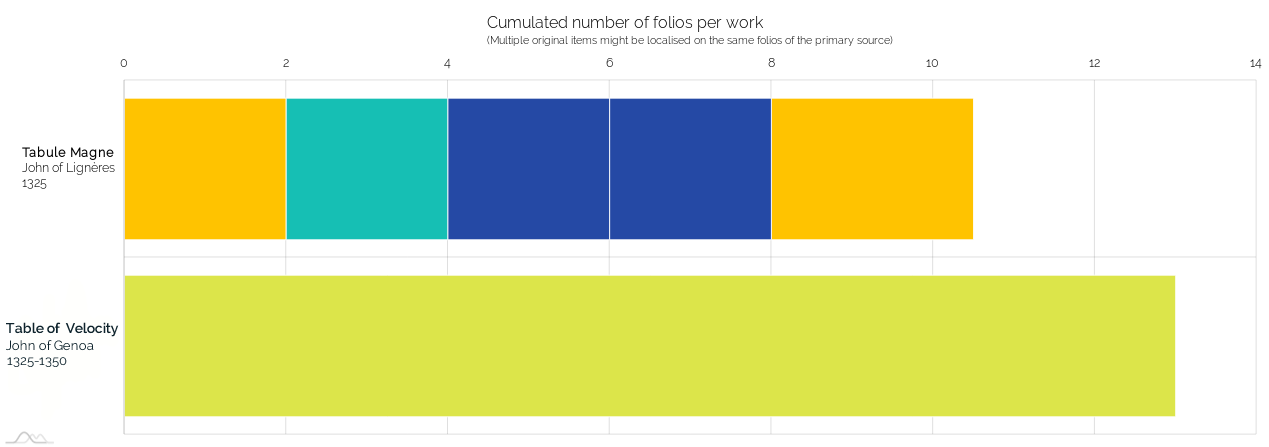
\includegraphics[width=16cm]{Images/Visualisations/Primary_source-Stacked.png}
	\caption{Visualisation du nombre de folios accumulé dans une source primaire}
\end{figure}

Le deuxième état de la visualisation présente les \ois, non plus comme accolés les uns aux autres, mais distribués horizontalement en fonction de leur foliotation. Il est ainsi possible de repérer si plusieurs tables ont été réunies sur les mêmes feuillets, ou encore si une même œuvre a été fractionnée à divers endroits de la source primaire. Cette visualisation révèle également si le copiste ou l'éditeur a entremêlé des tables provenant de plusieurs œuvres, de manière à composer un contenu original\footnote{Des versions simplifiées des visualisations en format \html ont été ajoutées aux documents accompagnant ce mémoire.}.

\begin{figure}[H]
	\centering
	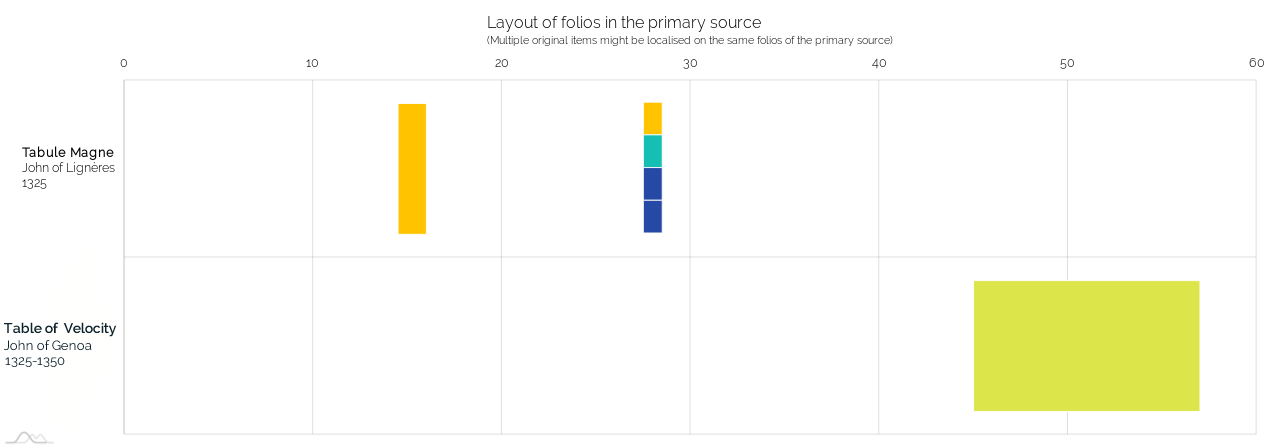
\includegraphics[width=16cm]{Images/Visualisations/Primary_source-Spread_out.png}
	\caption{Visualisation de la disposition des folios dans une source primaire}
\end{figure}

La visualisation ici sert à embrasser d'un seul regard des informations qui ne pourraient être obtenues ailleurs que par un examen attentif des sources primaires. Néanmoins, cette forme de représentation visuelle ne pourra être tout à fait significative qu'une fois que seront intégrés les autres types de contenus des sources astronomiques –~diagrammes et textes~– à la base de \dishas~; il sera alors possible aux chercheurs de déceler certains motifs structurels susceptibles d'apporter un nouvel éclairage sur les sources.

		\subsection{Représenter un milieu intellectuel~: le cas de la carte historique\label{HistoricalMap}}
Les visualisations ponctuelles, employées pour les pages de notices, ne représentant qu'un seul enregistrement de la base, sont utiles pour résumer graphiquement une donnée. Elles apportent un éclairage complémentaire aux seules métadonnées, mais ne peuvent remplacer une observation méthodique du matériel documentaire. La visualisation numérique accède à son véritable potentiel, lorsqu'elle agrège un grand nombre de données pour en dresser une synthèse visuelle. Plus les corpus représentés sont importants, plus ce genre de visualisation trouve son intérêt, donnant à voir ainsi des informations qu'il serait extrêmement ardu à obtenir autrement.

			\subsubsection{Représentation spatiale et chronologique}
La mise en évidence de milieux intellectuels est un enjeu de recherche central pour le projet \dishas. Le concept de milieu intellectuel peut être fondamentalement décrit par l'articulation d'un lieu et d'une époque~; leur représentation conjointe a souvent fait l'objet de réflexion, tant dans une perspective historique que pour des emplois plus éclectiques\footnote{GoogleMaps propose par exemple une fonctionnalité de \eng{timeline} permettant d'explorer les trajets réalisés avec l'application.~; par ailleurs, la bibliothèque de visualisation en carte \eng{Leaflet} propose huit \eng{plugins} pour la création de \g{carte temporelle}, généralement pour figurer des itinéraires.}. De nombreux historiens se sont attachés à proposer des solutions pour résumer au sein d'une même forme graphique le temps et l'espace~: on peut citer des initiatives aussi diverses que le \eng{Chronological Chart of Ancient, Modern and Biblical History} de Sebastian C. Adams publié en 1871 qui mêle histoire profane et religieuse sur une période de près de 5000 ans\footnote{\cite{AdamsSynchronologicalChart}} ou encore que l'encyclopédie et atlas digital \eng{TimeMaps} qui propose une série de cartes thématiques sur différentes époques de l'humanité.

Si la carte et la frise chronologique sont des moyens d'expression privilégiés de l'étude en \shs, leur articulation pose plusieurs problèmes, notamment dans une perspective de synchronicité. Bien souvent, le problème a été éludé en proposant une juxtaposition de cartes, chacune représentant une période définie\footnote{Comme la plateforme \emph{GeaCron} créée en collaboration avec l'Université Rey Juan Carlos (\cite{WorldHistoryMaps}) ou l'atlas \eng{TimeMaps}}, ou en figurant à l'aide de symboles visuels (flèches, zones colorées, etc.) des mouvements ou événements particuliers\footnote{À l'instar des nombreuses cartes du Musée national de l'histoire de l'immigration~: \cite{CartesMuseeNational}.}. L'irruption des techniques numériques dans le champ de la cartographie a ouvert les possibilités de visualisations~: en laissant l'utilisateur interagir avec les variables à représenter, il est possible de construire des cartes sur mesure\footnote{À propos d'un projet pionner en la matière, l'atlas élaboré par Éric Guichard en 1999~: \g{L’atlas \p permet à l’utilisateur de choisir tant les variables qu’il souhaite voir projetées sur la carte, que d’influer sur le mode de discrétisation des données. Il devient alors possible de générer une multitude de cartes, adaptées aux besoins du lecteur ou du chercheur, ce qui revient à créer un outil dont les fonctions ne sont pas reproductibles par un atlas papier, qu’il serait de toute façon impossible de publier.} \cite{massotDessinerActeursHumanites2018}}\footnote{Les cartes interactives créées par Étienne Côme pour visualiser les flux liés aux transports en communs sont très éclairantes à ce sujet~: \cite{comePortfolioEtienneCome}.}, mettant au jour des relations entre les données qui n'auraient pu être prévues avant la conception de la visualisation.

			\subsubsection{Réalisation d'une carte temporelle}
Afin de représenter la diffusion des textes et la circulation des paramètres astronomiques, l'idée de construire une visualisation combinant carte et frise chronologique s'est donc rapidement imposée. La visualisation en carte a en outre l'avantage d'harmoniser les différentes granularités de description de la donnée~: les entrées de la table \eng{Place} \g{Paris} et \g{Collège de Sorbonne} apparaîtront ainsi côte à côte, bien qu'ils constituent deux enregistrements tout à fait disjoints dans la \bdd. Toutefois, d'autres interrogations surgissent en parallèle, en particulier liées à la représentation d'entités placées sur un même lieu.

L'ajout de la dimension temporelle soulève en outre des questionnements spécifiques~: comment figurer le temps sur une carte~? Est-il préférable de pouvoir sélectionner une période ou une date ponctuelle~? Comment symboliser des objets –~sources primaires, paramètres~– n'étant pas directement (ou parfois même aucunement) liés à un lieu~? Par quels moyens peut-on représenter des données temporelles et spatiales parfois imprécises, sans induire l'utilisateur en erreur~? La visualisation qui a été élaborée tente de répondre au mieux à ces interrogations.

Cette visualisation en carte temporelle a été conçue pour être polyvalente et s'adapter à la représentation de différentes variables. Pour l'instant, elle a été implémentée sur la page de notice des \ois et sur la page d'accueil de la navigation historique. Il est prévu qu'elle puisse servir à la présentation des paramètres astronomiques. Nous prendrons pour sa description la version de la page \eng{Historical navigation}.

La visualisation se divise en deux parties fonctionnant de manière synchrone~: une carte géographique sur le dessus où figure l'ensemble des œuvres et des manuscrits de la \bdd~; sur le dessous, une carte de chaleur représente l'ensemble de la période couverte par les entités de la base. Une barre de sélection comportant deux curseurs sert de lien entre les deux cartes. La saturation de la couleur sur le dessous symbolise les périodes les plus prolifiques~; le jaune correspondant aux créations d'œuvres, le rouge aux copies/éditions de sources primaires. Les repères sur la carte représentent quant à eux les lieux de création et copie/édition de ces mêmes entités. Le rouge et le jaune gardent les mêmes références, tandis que l'orange indique un mélange entre œuvres et sources. Le diamètre des points quant à lui signale un plus ou moins grand nombre d'entités à représenter. L'utilisateur peut, au survol sur ces points et sur les bandes de la carte de chaleur, voir le nombre d'œuvres et de sources primaires correspondant au composant concerné.

\begin{figure}[h!]
	\centering
	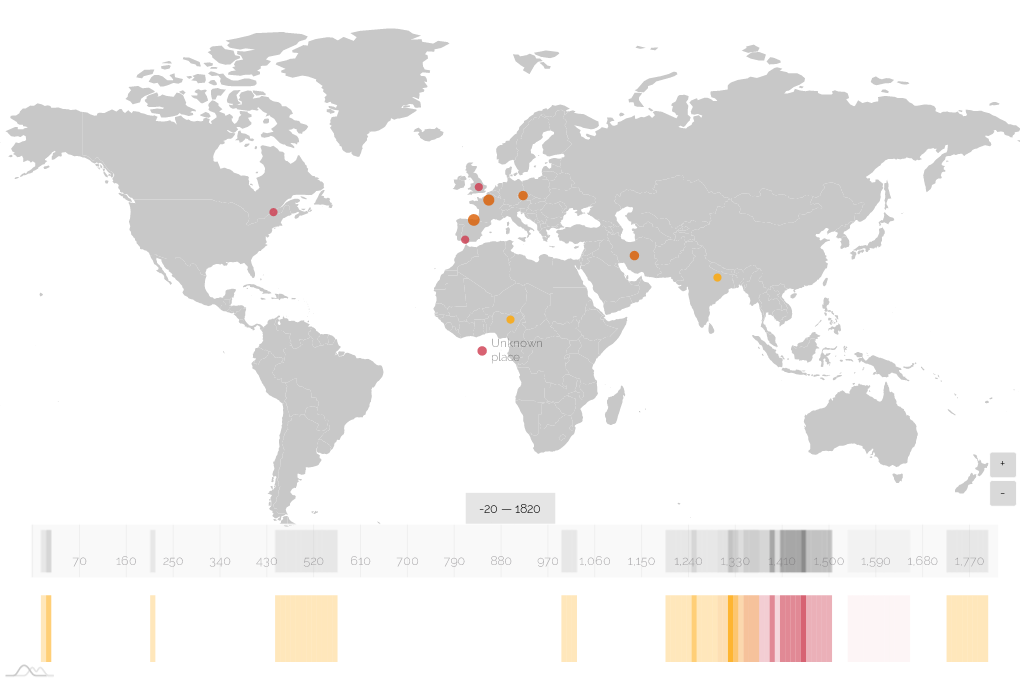
\includegraphics[width=16cm]{Images/Visualisations/Historical_navigation-All.png}
	\caption{Carte temporelle de la page \eng{Historical navigation}}
\end{figure}

La première remarque qui doit être faite concerne la visualisation des sources primaires. En effet, la source primaire n'est pas spatialisée dans la \bdd, seul l'\oi est associé à un lieu. Dans la mesure où il est plus logique d'accéder à la table astronomique par le biais de son contenant, il a été choisi de ne représenter sur cette page que des sources primaires, bien que ce ne soient en réalité que des \oi qui apparaissent sur la carte\footnote{Pour la visualisation des paramètres astronomiques, le même procédé pourra être repris de manière à faire apparaître sur une carte les sets de paramètres associés à des \ois.}. Cela signifie qu'une source primaire dispose potentiellement de plusieurs points sur la carte, dans le cas où elle n'aurait pas été produite à un unique endroit.

Étant donné que cette visualisation a été pensée comme un portail, chaque repère sur la carte est cliquable de façon à faire apparaître au-dessous de la visualisation des liens vers les entités concernées. Il est également prévu de rendre cliquables les différentes zones de la carte de chaleur, permettant ainsi d'accéder à la donnée par le biais chronologique comme spatial. Cependant, certaines entités ne sont associées à aucun lieu dans la base, mais elles doivent tout de même être rendues accessibles. Pour pallier cette difficulté, tous les enregistrements ne disposant pas d'information géographique ont été artificiellement situés aux coordonnées 0,0~; une annotation sur la carte précise qu'il s'agit d'une \g{\eng{Unknown place}} pour éviter toute confusion.

\begin{figure}[h!]
	\centering
	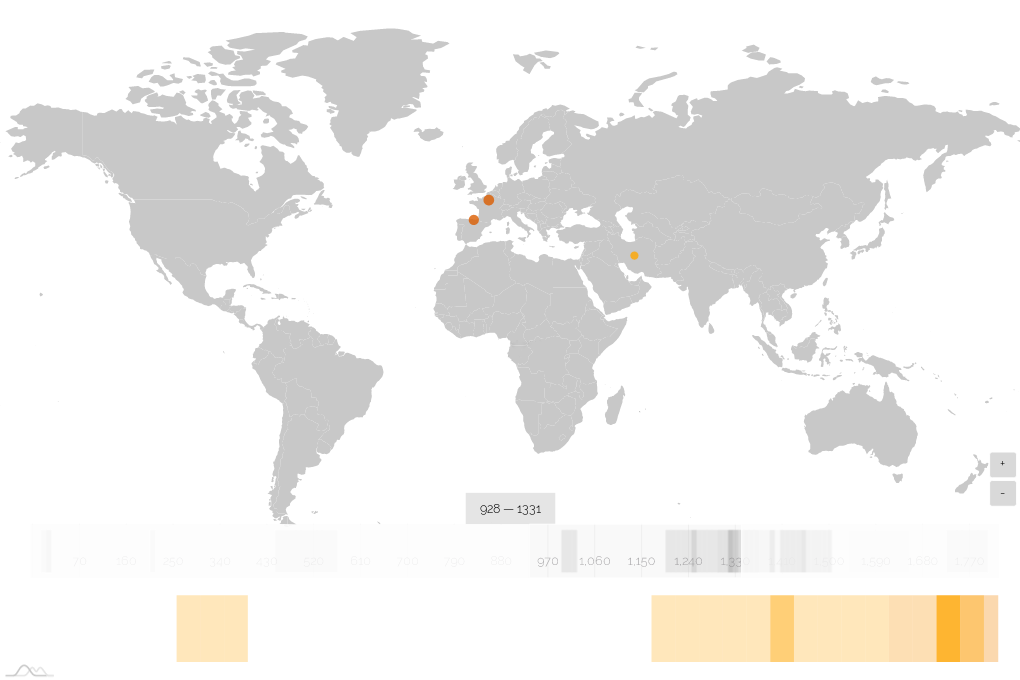
\includegraphics[width=16cm]{Images/Visualisations/Historical_navigation-Time_range.png}
	\caption{Sélection d'une période sur la carte temporelle}
\end{figure}

Lorsque l'utilisateur effectue une sélection grâce aux curseurs mis à sa disposition, les données affichées sur la carte sont mises à jour~: le diamètre, la couleur et les informations au survol des points évoluent\footnote{Pour le détail du code permettant ces modalités d'affichage, voir en annexes \ref{historical-map}.} en même temps qu'un agrandissement est effectué sur la frise au-dessous. En revanche, le zoom sur la carte n'entraîne pas d'actualisation de la carte de chaleur pour des raisons d'impossibilités liées à la technologie utilisée pour la visualisation\footnote{La bibliothèque JavaScript \eng{AmCharts} ne dispose pas de moyen d'accéder aux informations relatives à la portion de carte affichée à l'écran de l'utilisateur.}.

Cette visualisation illustre les possibilités permises par la visualisation numérique. En représentant simultanément l'ensemble des données de la base, les corrélations entre elles sont rendues manifestes, alors qu'elles restaient auparavant inaccessibles. Différents choix éditoriaux ont été faits pour la figuration des données~; ils conditionnent la manière dont sont appréhendées les informations. Il est en ce sens du rôle du concepteur de tâcher de biaiser le moins possible les représentations, pour permettre aux chercheurs de tirer un maximum de profit de ce genre de réalisations numériques.\\

Ainsi, la mission de la plateforme publique vis-à-vis des chercheurs de \dishas constiste en grande partie à réveler les interactions contenues dans la \bdd, au travers de visualisations analytiques, comme de fonctionnalités permettant de réunir des ensembles cohérents dans le corpus numérisé, à l'instar des modalités de recherche et de l'ouverture des métadonnées au sein des notices. Si le \eng{back office} propose des interfaces fonctionnelles pour la gestion des données, le \fo doit offrir des interfaces propres à manifester leurs correspondances et interconnexions au sein de la base, dans le but d'accompagner au mieux le travail de recherche.

\clearemptydoublepage

\chapter[Assurer la réutilisation du corpus numérique]{Exposition des données brutes~: assurer la réutilisation du corpus numérique}
Les deux précédents chapitres se sont attachés à décrire comment présenter et mettre en relation les données au sein du \fo. Si ces formes de médiatisation sont nécessaires pour donner du sens au corpus numérique, elles le rendent également univoque. En effet, ces modes d'exposition constituent un accès indirect à la donnée~; l'élaboration d'une plateforme en ligne offre en cela une vision réductrice de la donnée. Les ressources numériques, une fois incorporées à un discours qui les décrit et intégrées à une interface graphique, sont rendues en grande partie inutilisables. Dans une perspective de conformité avec les principes \fair, un effort de médiation doit être fourni pour rendre accessible la donnée brute, de manière à permettre la réexploitation du corpus numérisé.

	\section{Accessibilité des données brutes}
La plateforme de \dishas a l'ambition de servir de portail de partage de données dans l'objectif de favoriser la pratique de l'\eng{open data} en histoire de l'astronomie. La mise à disposition du matériau numérique non transformé offre au public la possibilité de réutiliser les ressources scientifiques~: cette exposition des données peut s'opérer à plusieurs niveaux.

		\subsection{Modalités d'accès à la donnée}
			\subsubsection{Entrepôts de données pérennes}
En France, plusieurs infrastructures s'attachent à accompagner les chercheurs dans l'exposition et la pérennisation des données de recherche. Le \cines, établissement public placé sous la tutelle du Ministère de la Recherche et de l'Innovation, s'est fixé depuis sa création en 1999, une mission d'archivage des documents électroniques produits par la communauté scientifique. L'archivage pérenne concerne non seulement la gestion de l'obsolescence des formats et des environnements logiciels, mais également l'assurance de l'accessibilité des ressources\footnote{\g{L’archivage numérique pérenne n’est pas non plus l’ultime étape du stockage des données avant l’oubli ou la perte définitive} \cite{ConceptArchivageNumerique}}. De toute évidence, les missions de conservation et de communication sont complémentaires et doivent être envisagées ensemble, l'une n'ayant pas de sens sans l'autre. Le \cines insiste en particulier sur l'importance de la description des contenus numériques à l'aide de métadonnées~: en effet, sans métadonnée, la finalité d'un document peut être perdue, celui-ci devenant ainsi rapidement inexploitable.

La \textsc{tgir} Huma-Num est le second acteur majeur pour la valorisation des données de recherche, elle travaille par ailleurs en collaboration avec le \cines. Afin d'assurer un accès persistant et interopérable aux ressources numériques, Huma-Num a mis en œuvre un système d'exposition des données intitulé Nakala. Nakala est une \bdd triplestore\footnote{Un triplestore est une \bdd graphe utilisée pour le stockage et la récupération des triplets \rdf~; le langage de requêtage d'un triplestore est le langage \sparql.} où peuvent être entreposés les corpus de recherche~; le \sparql \eng{endpoint} de Nakala permet de récupérer ces données numérisées, chacune étant signalée grâce à un identifiant pérenne, assurant leur trouvabilité dans le temps. Le recours aux standards du Web de données (lié à l'utilisation d'un triplestore), reposant sur des technologies et méthodes standardisées, permet de faciliter à la fois la récupération des données, mais aussi leur réutilisation. En effet, de nombreuses formes de valorisations s'appuient sur le format \rdf, notamment le moissonnage des métadonnées par des services spécialisés comme Isidore ou Gallica, ou encore la réalisation de visualisation de données\footnote{\cite{NAKALAParHumaNuma}}.

			\subsubsection{Exposition de données courantes}
Cependant, cette forme d'exposition des données brutes implique l'établissement d'un corpus défini, exploitable en l'état. La \bdd de \dishas est encore sujette à de nombreuses modifications et le travail de numérisation des sources est encore loin d'être achevé. Il est donc nécessaire de trouver des voies d'exposition de cette donnée \g{intermédiaire}~; avant la pérennisation définitive du corpus dans Nakala, l'interface publique de \dishas doit servir de plateforme de diffusion pour les données en train d'être façonnées par les chercheurs. L'application Web du projet ne se substitue pas à Nakala, leurs missions sont complémentaires et les développements prévus pour \dishas se doivent de ne pas entrer en concurrence avec les services proposés par Huma-Num.

Dans le but de donner un accès direct aux données de recherche, différentes fonctionnalités ont été implantées~: Malcolm Hamelin, stagiaire du projet d'avril à juillet 2019, a été chargé de mettre en place une \api ainsi que le moteur de recherche ElasticSearch sur la \bdd\footnote{Pour davantage de détails concernant l'implémentation, voir section \ref{Elastic}.}. L'\api permet aux utilisateurs et aux machines de communiquer directement avec la \bdd de \dishas~; par le biais d'une interface en ligne de commandes, il est possible de récupérer, de modifier ou d'ajouter des données dans la base\footnote{Quatre actions peuvent être effectuées par l'\api. Ce sont les opérations \crud, correspondant aux différentes façons d'interagir avec une \bdd~: ajout, modification, suppression et lecture de données.}. L'\api est à destination principale des chercheurs, leur permettant d'intégrer massivement des données en contournant l'interface graphique~: en effet, l'utilisation de l'\api requiert un \eng{token} d'identification, défendant au grand public de rentrer n'importe quelle donnée dans la base.

ElasticSearch en revanche, fonctionne sur un duplicat de la \bdd~; il n'est donc pas possible d'ajouter des données à la base relationnelle par le biais d'ElasticSearch. Son utilisation principale concerne la récupération des données de \dishas et leur exposition à un public plus large que la seule équipe de recherche du projet. En effet, la base d'ElasticSearch peut être interrogée à la manière d'une \api, de façon à ouvrir l'accès aux données brutes de \dishas à des utilisateurs extérieurs comme à d'autres plateforme en ligne. Les données récupérées par le biais de l'\api et d'ElasticSearch sont encodées en \json, format largement employé, facilitant ainsi leur réutilisation.

\begin{figure}[h!]
	\centering
	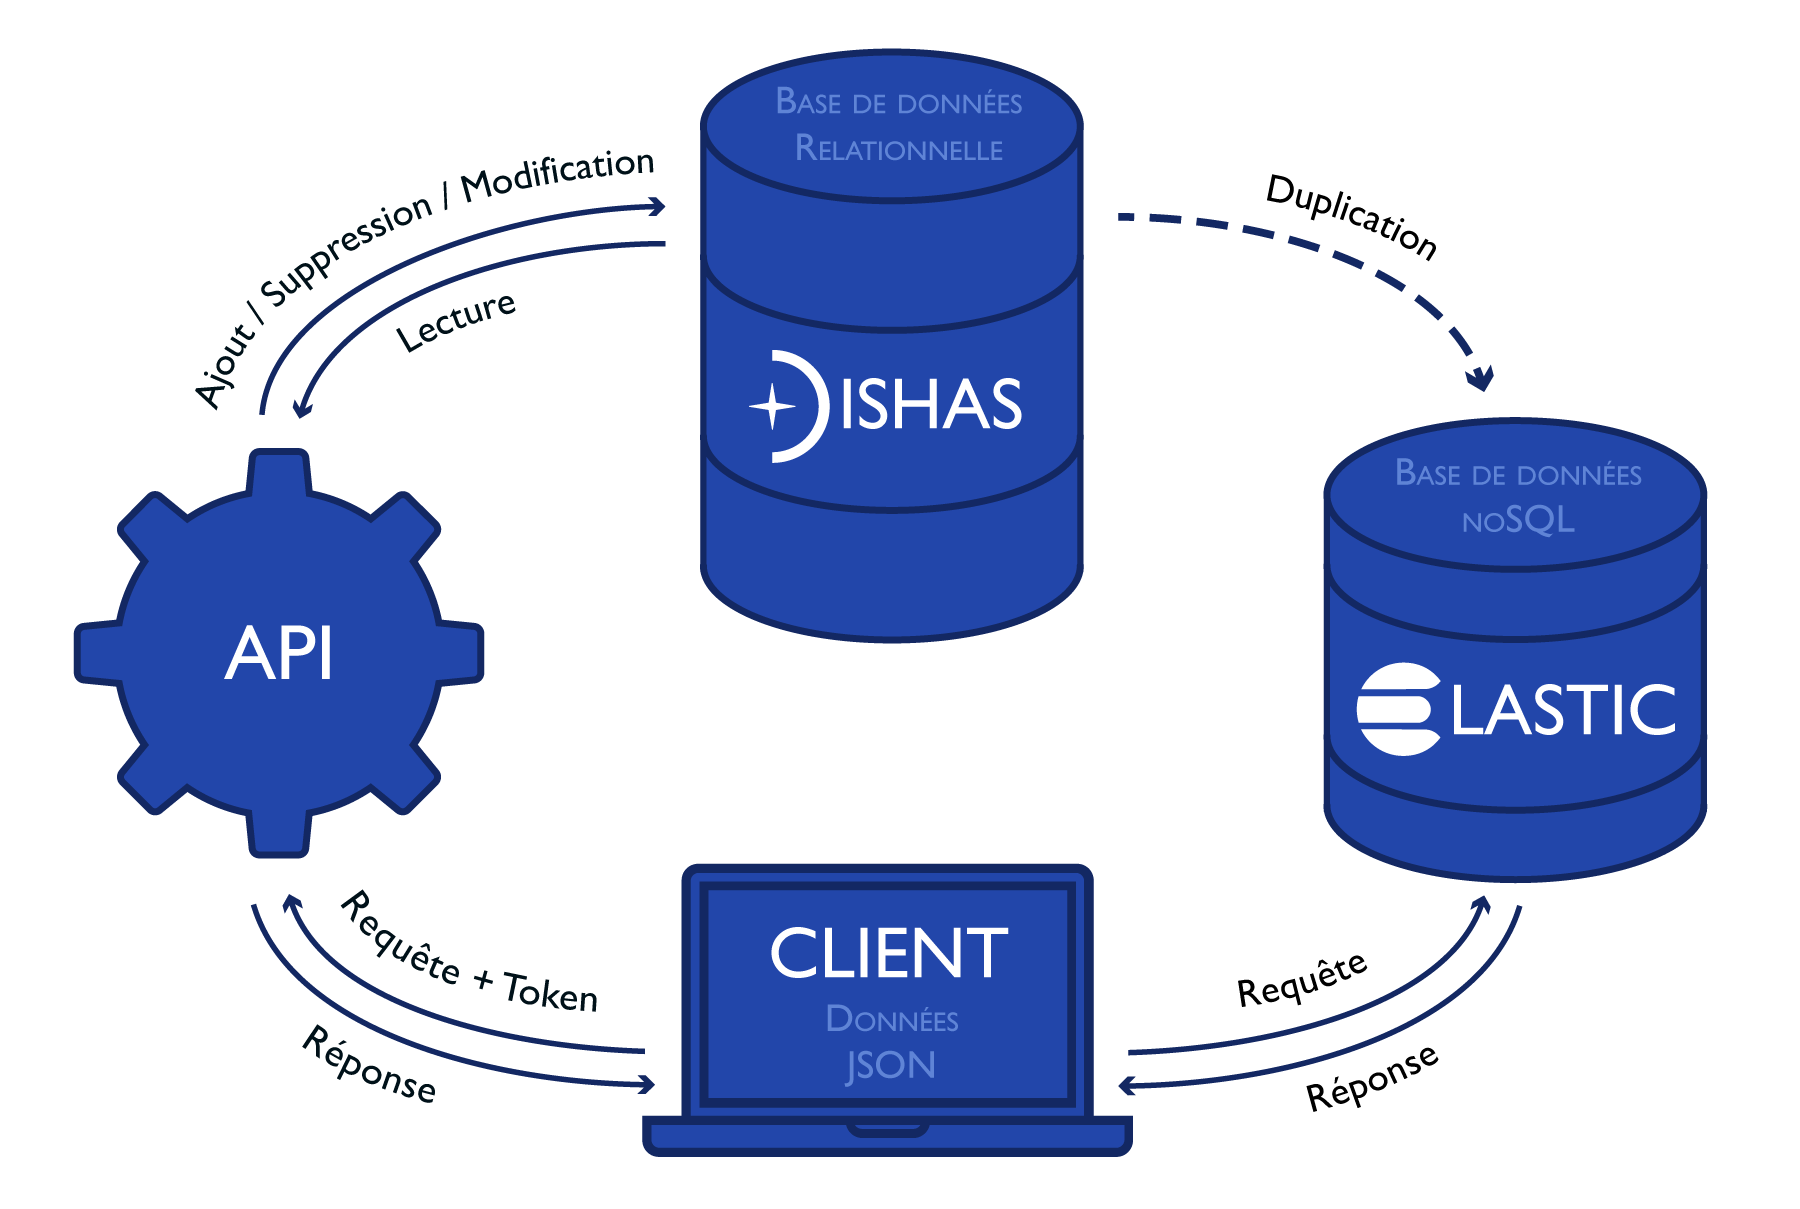
\includegraphics[width=14cm]{Images/BDD-ElasticSearch-API.png}
	\caption{Interaction entre la \bdd de \textsc{dishas}, l'\textsc{api} et ElasticSearch}
\end{figure}

		\subsection{Fonctionnalités implémentées dans l'interface publique}
La plateforme publique de \dishas n'intègre pour l'instant que peu d'accès à la donnée brute~: seuls deux endroits du \fo exposent une partie des données nécessaires à leur constitution.

La barre latérale présente sur les pages de notice, comporte plusieurs icônes à la disposition de l'utilisateur. L'un d'entre eux permet le téléchargement en \json de l'ensemble des métadonnées affichées. Toutefois, il s'agit d'un objet qui a été formaté pour répondre aux besoins de mise en forme imposés par le \eng{template} de la barre latérale, il serait donc difficile à un utilisateur d'exploiter véritablement ce matériau. Il est prévu de réviser cette fonctionnalité.

L'interface de recherche quant à elle, repose sur la \bdd d'ElasticSearch~; lorsque l'utilisateur soumet une recherche plein-texte, une requête est expédiée au serveur d'ElasticSearch\footnote{Pour plus de précision sur les méthodes de requêtes asynchrones à ElasticSearch, voir section \ref{Ajax-Elastic}.}. Les informations renvoyées par le serveur sont ensuite disposées dans un tableau de résultats pour une présentation graphique satisfaisante~; cependant, un bouton sous la barre de recherche propose à l'utilisateur de copier la requête envoyée à ElasticSearch dans son presse-papier. En collant cette requête dans la barre d'adresse d'un navigateur, la réponse en format \json telle que renvoyée par le serveur est rendue disponible.

Ces fonctionnalités restent relativement rudimentaires et peu documentées. De futurs développements du \fo devront s'attacher à rendre les données de recherche davantage accessibles~; néanmoins, ce travail se concentra principalement sur la documentation des outils déjà existants. En effet, il existe d'ores et déjà des interfaces tout à fait fonctionnelles pour le requêtage de données, l'enjeu est avant tout d'expliquer au public comment utiliser ces outils. Ainsi, il est possible d'imaginer que des tutoriels pour l'utilisation d'ElasticSearch puissent être intégrés aux pages publiques, sous forme de ressource à télécharger ou de contenu à part entière. La question des exports des données devra également être réfléchie plus avant, notamment vis-à-vis du choix des informations à extraire et de leurs modélisation à l'intérieur d'une chaîne \json.

	\section{Exposer les méthodes~: documentation et maintien de code}
La seule mise à disposition des données au public ne suffit pas à favoriser leur réutilisation. En effet, les corpus numériques, isolés de leur contexte de production, sont dénués de signification propre~: pour promouvoir leur usage, il est important que les concepteurs de la donnée et des outils qui l'accompagnent, fournissent des documents explicitant leurs pratiques. Ce contenu est destiné aux utilisateurs extérieurs au projet, mais plus encore aux futurs et actuels développeurs de l'application de \dishas. En outre, cette documentation doit s'appuyer sur du code de qualité, de manière à ne pas nécessiter de modifications majeures lors de la reprise du projet par une nouvelle équipe d'ingénieurs.

Les développements réalisés au cours de mon stage s'efforcent de respecter les bonnes pratiques énoncées ci-après, de multiples ajustements seront toutefois probablement nécessaires en vue de leur mise en production.

			\subsection{Lisibilité et documentation}
				\subsubsection{Intelligibilité du code}
Une des premières exigences des développements pour la constitution d'applications solides et réutilisables concerne la lisibilité du code. L'indentation, la suppression des redondances ou l'utilisation de sucre syntaxique\footnote{Méthode de clarification de la syntaxe programmatique à l'aide de raccourcis et tournures de code allégées.} sont autant de moyens de rendre la lecture du code plus aisée. Pour le développement des interfaces de \dishas, plusieurs relectures du code ont permis d'en alléger la structure et de retirer des pans entiers de procédures inutiles. Des noms de variables signifiants ont été choisis de manière attentive, dans le but de participer à l'intelligibilité du code. L'emploi de la bibliothèque jQuery enfin, disposant d'une syntaxe plus compréhensible que le JavaScript simple\footnote{Aussi appelé JavaScript \eng{vanilla}.}, a en outre aidé à la clarté des développements, grâce aux nombreux raccourcis et méthodes intégrés à la bibliothèque.

\begin{figure}[H]
\begin{lstlisting}
/* VANILLA JAVASCRIPT */
if (document.getElementById("sidebar").getAttribute("isOpen") === "false") {
        document.getElementById("toolbar").classList.add("open-toolbar");
}
\end{lstlisting}
\begin{lstlisting}
/* JQUERY */
if ($("#sidebar").attr("isOpen") === "false") {
    $("#toolbar").addClass("open-toolbar");
}
\end{lstlisting}
\caption{Différence de syntaxe entre Javascript simple et jQuery}
\end{figure}

				\subsubsection{Exhaustivité de la documentation}
La documentation des développements est d'une importance capitale pour leur maintenance et leurs réemplois ultérieurs. Le code, par-delà la question de la lisibilité, requiert d'être explicité pour être rendu véritablement accessible, et par là même, réutilisable. La documentation doit s'insérer à différents niveaux du développement pour assurer des explications tant du point de vue de l'architecture globale de l'application, que des plus petits composants de la syntaxe programmatique.

\begin{figure}[H]
\begin{lstlisting}
/* EXEMPLE D'EXPLICITATION DU CODE */
if ($("#sidebar").attr("isOpen") === "false") {
// Si la valeur de l'attribut "isOpen" de l'élément HTML avec pour identifiant "sidebar" est égale à "false"
    $("#toolbar").addClass("open-toolbar");
    // alors ajouter la classe "open-toolbar" à l'élément HTML avec pour identifiant "toolbar"
}
\end{lstlisting}
\caption{Exemple de commentaires de code intralinéaires}
\end{figure}

Au cours de la conception du \fo, des commentaires intralinéaires ont été ajoutés pour expliciter les passages les plus ardus du code. Chacune des fonctions élaborées a été en outre documentée~: leur utilité, les arguments nécessaires à leur exécution et leur fonctionnement ont systématiquement été notifiés. Afin de garder des traces des différentes réalisations, chaque \eng{commit}\footnote{Sauvegarde d'un état d'avancement du travail.} a été associé à un message détaillant précisément les modifications et ajouts effectués sur le code. Enfin, des notes plus extensives ont été rédigées à l'achèvement du travail, exposant avec précision la nature des développements et les instructions pour les reproduire au besoin\footnote{Ces documents sont reproduits aux annexes \ref{ElasticSearch}, \ref{Branche} et \ref{AmCharts}.}.

			\subsection{Gestion de \eng{bugs}}
Pour assurer une expérience positive liée à l'utilisation de la plateforme, les erreurs d'exécution du code doivent être évitées au maximum. Le chargement correct et rapide des pages, le bon fonctionnement des composants de l'interface ou encore le comportement approprié des différents modules sont des facteurs influençant non seulement l'expérience utilisateur, mais également l'exposition générale des données du projet. L'efficacité des interfaces est la conséquence directe de l'anticipation et la correction d'erreurs informatiques. Le maintien régulier du code est souvent un argument retenu par les développeurs pour attester de la stabilité d'un projet~; la gestion des \eng{bugs} doit donc faire partie intégrante du processus de développement.

				\subsubsection{Prévenir les erreurs}
Plusieurs méthodes peuvent être mises en place pour anticiper la survenue d'erreurs. En premier lieu, l'utilisation de bibliothèques et d'infrastructures logicielles\footnote{Aussi appelés \eng{frameworks}. Un \eng{framework} est un ensemble cohérent de composants logiciels servant de cadre à la conception d'une partie ou de la totalité d'une application.} éprouvées simplifie le travail de correction tout en assurant un environnement stable pour l'implémentation de nouvelles fonctionnalités\footnote{\g{\eng{As it has already been invented, and is not considered to have any operational flaws, an attempt to reinvent it would be pointless and add no value to the object, and would be a waste of time, diverting the investigator's resources from possibly more worthy goals.}} \cite{ReinventingWheel}}. Elles garantissent que les différentes briques logicielles constituant l'application bénéficient de mises à jour régulières, ou \emph{a minima} d'un support de la communauté de programmeurs utilisant le même outil.

Les modèles –~ou \eng{template}~– aident également à la maintenabilité du code. Les modèles permettent d'appliquer des traitements similaires à un ensemble de pages partageant des structures communes. Contentrant dans un seul fichier l'ensemble des propriétés de multiples interfaces, ils en assurent la cohérence mais facilitent également leurs modifications. De manière générale, la mutualisation du code allège le travail de développement et fournit un environnement de travail plus stable. La réunion de morceaux de code cohérents au sein de fonctions enfin, simplifie leur réutilisation et participe à construire une application plus robuste. Tous ces éléments façonnent une logique globale pour la plateforme, qui prévient un maximum de dysfonctionnements programmatiques.

				\subsubsection{Recettes fonctionnelles}
La conduite de tests est également essentielle à la construction d'une application. Différentes méthodes permettent d'éprouver le fonctionnement du code~: l'intégration continue, par exemple, consiste en la conduction de tests à chaque nouvelle version du code, de manière à repérer et corriger immédiatement les éventuelles régressions ou erreurs. Cette approche vise à réduire les problèmes d'intégration. Les tests unitaires quant à eux, permettent d'évaluer le bon fonctionnement d'une partie précise du code. Il est préconisé de les rédiger simultanément au code, de manière à les faire correspondre parfaitement et d'éviter ainsi la propagation d'erreur.

La mise en œuvre de telles procédures requiert de nombreuses heures de développement, et l'équipe technique chargée du projet \dishas ne compte, à l'heure actuelle, que deux membres~; le déploiement systématique de tests n'a donc pas pu  être encore intégré au processus de travail des ingénieurs. De manière à assurer la viabilité de l'application, l'équipe technique a en revanche recours aux recettes fonctionnelles. Les recettes fonctionnelles consistent à évaluer la conformité du produit fini avec le cahier des charges initial. Un ensemble de points est identifié~; une série de tests est définie pour chacun de ces points, afin de vérifier l'adéquation de leurs fonctionnements avec les spécifications originales. Par exemple, pour chaque contenu texte des interfaces, il sera testé si l'utilisation de caractères spéciaux ou d'alphabets étrangers ne corrompt pas l'affichage. Toutefois, ces vérifications ne sont pas encore automatisées et leur déploiement nécessite d'être optimisé dans le futur.\\

L'exposition des données brutes et des méthodes permettant leur utilisation influe sur la diffusion des sources scientifiques du projet. La description technique du corpus numérique doit être mise en avant au sein de la plateforme publique, mais également à l'intérieur même du code sur lequel elle s'appuie, sous la forme de documentation rigoureuse. Si le public susceptible d'être intéressé par cet aspect de la donnée ne constitue qu'une part minoritaire des utilisateurs, l'importance de la communication sur les ressources numériques et sur leurs outils est capitale. En effet, cette forme de médiation assure aux données de recherche un cycle de vie dépassant le simple cadre de \dishas, en préservant leur caractère polyvalent. La médiation des données brutes représente également une valorisation du travail des ingénieurs et des chercheurs~; l'exposition du processus d'élaboration de ces ressources participent à faire fructifier les réalisations numériques du projet.

\clearemptydoublepage

\part{Traitement technique de la donnée et management des interactions}
\chapter{Gestion de projet}
	\section{Dialogue entre recherche et ingénierie}
Le développement du projet \dishas s'inscrit à de nombreux égards dans la pratique des humanités numériques~; son aboutissement est le fruit que d'un partenariat étroit entre équipe de recherche et équipe technique. De nombreux enjeux peuvent être soulevés par une telle collaboration~: afin d'assurer le déroulement optimal des réalisations du projet, il est intéressant de comprendre quelles problématiques peuvent émerger du dialogue entre ingénieur et chercheur.

		\subsection{Coopération dans le domaine des humanités numériques}
La place des humanités numériques au sein de la communauté de recherche en sciences humaines a souvent été l'objet de débat. Le caractère protéiforme de leur pratique et la multiplicité de leurs applications rendent leur définition malaisée~: cette difficulté à circonscrire les humanités numériques a parfois été l'origine d'incompréhension parmi les acteurs des \shs. Incompréhension notamment vis-à-vis du rôle des ingénieurs numériques au sein des projets de recherche~: tantôt perçus comme des simples exécutants\footnote{\g{La contribution des techniciens est rarement analysée en tant que telle (du point de vue d’une sociologie du travail scientifique), mais presque toujours en fonction de leur contribution aux processus de production des connaissances scientifiques (du point de vue d’une sociologie de la connaissance)} \cite[p.~163]{millerandScienceReseau2012}}, tantôt considérés comme ayant la solution à tout problème, les ingénieurs peuvent avoir du mal à se positionner\footnote{\g{\eng{In these digital times, IT tools are no longer an auxiliary science to history. Integrating them into the “established procedures” has got to be the major challenge facing the discipline in the coming years.}} \cite[§~40]{heimburgerHasHistorianCraft2012}}. Ces facteurs rendent complexe l'établissement d'un dialogue fécond entre chercheur et \g{technicien}\footnote{\g{Le paysage universitaire français a en effet pour particularité d’être structuré sur une séparation radicale entre recherche d’un côté, et services de l’autre. Cette dichotomie se retrouve au niveau des individus avec un cloisonnement étanche entre différents corps de la fonction publique, et au niveau des structures avec l’opposition bien connue entre unités de recherche et unités de service.} \cite[p.~44]{dacosEtatLieuxPositionnement2013}}.

Plutôt que de renforcer la dichotomie entre recherche et numérique, c'est la mise en commun des savoirs qui doit être visée dans le but d'un enrichissement mutuel. D'une part, les chercheurs, en s'appropriant les techniques numériques, ouvrent l'horizon de leurs travaux scientifiques~; d'autre part, les ingénieurs qui continuent leur formation en sciences humaines, élargissent le champ de leurs réalisations. La distinction étanche entre les domaines d'expertise nuit à l'émergence de profils mixtes, susceptibles de surmonter le cloisonnement disciplinaire et d'être vecteurs d'innovation.

L'ingénieur en humanités numériques, par son interdisciplinarité, est ainsi au centre du processus de recherche~; il doit à la fois comprendre les enjeux scientifiques ainsi que les contraintes techniques. Les réalisations qu'il met en œuvre doivent être le fruit d'une collaboration étroite avec le chercheur, qui doit appréhender de son côté les enjeux techniques sous-jacents\footnote{\g{En résumant ces différents éléments, on peut suggérer que l’enjeu pour les spécialistes en informatique est de parvenir à faire voir les limites qu’ils fixent aux possibilités d’action de l’équipe comme indépendantes de leurs propres capacités.} \cite[§~21]{oberhauserCollaborationsEquivoques2016}}. Cette coopération permet de prévenir des choix techniques dommageables –~lorsque les enjeux scientifiques ne sont pas bien explicités ou compris~– comme d'éviter l'élaboration d'instruments qui finissent inutilisés –~lorsque les chercheurs ne s'approprient pas les outils.

\begin{quote}
	Si le chercheur ou l’enseigneur-chercheur ont la responsabilité d’impulser et de porter des axes de recherche novateurs, en véritables initiateurs du dialogue entre discipline et technique, l’ingénieur est le dialogue en acte. En véritable traducteur, il transmet des techniques, des méthodes, mais aussi conçoit et expérimente de nouveaux outils et guide le chercheur dans ses découvertes. Il est à l’interface entre les humanités, l’informatique et le design, en dialogue constant entre disciplines et techniques. Il sert de pont entre l’idée du chercheur et l’innovation technique, la recherche et son application, son incarnation concrète.\footnote{\cite[p.~3]{massotDessinerActeursHumanites2018}}
\end{quote}

Le rôle de l'ingénieur numérique n'est donc pas tant celui d'un intermédiaire –~mettant en œuvre des moyens pour répondre à une demande~– que d'un médiateur, accompagnant les pratiques scientifiques dans leurs mutations liées à l'apport des technologies numériques\footnote{\g{Loin d’être un simple développement technologique ayant un impact sur le processus de recherche et de visualisation des données en sciences humaines et sociales, les humanités numériques nous amènent à repenser le sens même de la recherche et, par conséquent, l’ensemble du modèle de production et de circulation du savoir à l’époque de l’édition numérique.} \cite[§~3]{sinatraChapitreHistoireHumanites2014}}. Dans cette mesure, l'ingénieur se doit de ne pas être un simple exécutant, mais aussi un acteur décisionnel, pour aider à définir quels développements seront les plus adaptés au travail du chercheur.

		\subsection{Processus de conception des interfaces}
La conception des interfaces publiques de la plateforme de \dishas est le fruit de nombreux allers-retours entre exigences scientifiques et contraintes techniques. À la suite d'un examen approfondi de la \bdd et de nombreuses discussions à propos du corpus de recherche, une première ébauche des pages du \fo a pu être dressée. Aucun cahier des charges préalable n'a orienté ou déterminé le choix des réalisations~; au contraire, c'est l'appropriation progressive des enjeux scientifiques sous-tendant au projet, qui a présidé à l'élaboration de la plateforme publique. L'évolution graduelle des développements s'est ensuite opérée au travers de deux phases complémentaires, répétées de manière itérative~: une phase projective de description détaillée des interfaces à réaliser, et une phase démonstrative de confrontation des interfaces (concrétisées ou anticipées) avec les membres de l'équipe pour ajuster les développements.

Les procédés exposés ci-après sont employés au sein de l'équipe de \dishas dans le processus de production numérique. Ces méthodes visent à favoriser la communication entre les chercheurs et les ingénieurs pour qu'en émanent des interactions fructueuses. Elles ont été implantées au fur et à mesure de l'avancée du projet, dans le but d'éviter de cloisonner le travail des membres de chaque équipe. Les paragraphes suivants constituent un retour d'expérience concernant l'élaboration de l'interface publique.

				\subsubsection{Séminaires numériques}
Chaque mois est organisé au sein de l'Observatoire un séminaire d'équipe orienté \dhu~: ce séminaire est alternativement animé par les membres du pôle numérique de \dishas et par des intervenants extérieurs. L'objet de ces séminaires varie, il s'agit autant d'exposer l'avancement de travaux de l'équipe d'ingénierie, que de présenter des instruments informatiques intéressants. À titre d'exemple, les quatre derniers séminaires ont porté sur~: l'assistant bibliographique Zotero, les interfaces du \fo\footnote{Le document de présentation utilisé lors du séminaire est reproduit en annexe \ref{PresentationSeminaire}.}, les différentes applications de l'édition avec \xml \textsc{tei} et l'implémentation des outils d'ElasticSearch. Ces séminaires sont l'occasion de faire se rencontrer les chercheurs et les ingénieurs pour échanger à propos des réalisations numériques, mais aussi pour accompagner une première prise en main de ces outils\footnote{\g{La conclusion à en tirer est que les chercheurs doivent d’abord connaître les logiciels développés pour eux, pas nécessairement qu’ils sachent programmer. Des logiciels puissants existent, il n’est pas toujours nécessaire de réinventer la roue. L’ignorance informatique des historiens doit être évitée, mais il est nécessaire de disposer d’une bonne culture informatique, autorisant un bon apprentissage des logiciels.} \cite[§~21]{clavertHistorienProgrammeur2012}}.

L'ingénieur doit tâcher de concentrer la discussion sur les points qu'il estime être les plus pertinents. Certains aspects trop techniques peuvent ainsi être éludés, tandis que les points concernant la représentation de l'information peuvent être davantage développés. Ainsi, les échanges lors de la présentation du \fo se sont notamment orientés sur le raffinement des visualisations de données~: les suggestions de chacun ont été évaluées et débattues, tant du point de vue de leur faisabilité que de leur intérêt, aboutissant à l'élaboration d'interfaces plus riches. Certaines propositions vis-à-vis de l'architecture de l'information dans le parcours de navigation ont par ailleurs été entièrement repensées, donnant lieu par exemple à la fusion des pages concernant les éditions et de celles relatives aux modèles mathématiques. Il a été évoqué enfin, la part active que doivent prendre les chercheurs dans la conception de la plateforme publique, en particulier dans la rédaction de textes introductifs pour les différentes pages de la navigation \footnote{\g{Nous abordons la question de la planification des tâches à accomplir et des objectifs à atteindre dans le cadre du projet, en montrant comment les efforts de coordination déployés par les chercheurs s’appuient de manière décisive sur les informations transmises par les spécialistes en informatique.} \cite[§~5]{oberhauserCollaborationsEquivoques2016}}.

				\subsubsection{Spécifications fonctionnelles}
L'établissement d'un document détaillant l'ensemble des développements planifiés a constitué une seconde phase dans le travail d'élaboration du \fo. La définition écrite des réalisations prévues vise plusieurs objectifs. En premier lieu, l'évaluation globale des moyens à mettre en œuvre pour leur concrétisation, mais aussi la constitution d'un document maître auquel se référer. Ce document\footnote{Ce document, réalisé dans le premier moi de mon stage, a été reproduit en annexe \ref{CahierDesCharges}.} est un cahier des charges fonctionnel où est décrite en détail chaque page de la plateforme publique. Il se présente sous forme de tableau où chaque rangée correspond à une page de l'interface, chaque colonne concernant quant à elle un aspect précis de cette page~:

\begin{itemize}
	\item une première colonne présente l'interface de manière générale~: son objectif, son architecture globale avec la description de ses différents composants ainsi qu'éventuellement des interrogations vis-à-vis de sa conception~;
	\item une deuxième colonne expose l'ensemble des données qui seront récupérées de la base pour l'affichage, en particulier pour les métadonnées requises dans les pages de notices~;
	\item une troisième colonne s'attache à expliciter précisément la visualisation de donnée apparaissant sur la page (si tel est le cas), tant dans son aspect visuel que dans ses enjeux intellectuels~;
	\item une quatrième colonne concerne les données nécessaires à la constitution de cette visualisation~;
	\item une cinquième colonne dresse la liste de tous les liens de redirection présents à l'intérieur de la page, composant ainsi le réseau dans lequel elle s'inscrit~;
	\item une dernière colonne détaille les corpus de données qui pourront être établit à partir de cette page. Cette partie concerne essentiellement les pages de notice, et fait référence aux \g{loupes} disposées sur la barre latérale de métadonnées\footnote{Leur fonctonnement est décrit plus en détail à la section \ref{OuvrirMeta}.}.
\end{itemize}

Ce document, en plus d'aider au cours du développement de la plateforme, fournit un support pour les remarques potentielles des chercheurs~; il doit donc s'efforcer de viser l'exhaustivité des descriptions, énoncées dans un style le plus limpide possible. Il constitue ainsi un socle commun sur lequel peut s'appuyer le dialogue entre utilisateurs et concepteurs. En s'assurant en amont que le projet numérique est en adéquation avec les attentes de l'équipe de recherche, il est possible mettre de côté les réalisations inutiles et d'identifier celles auxquelles il faut accorder la priorité.

Le cahier des charges fonctionnel, ainsi que les différentes étapes d'avancement des interfaces ont pu être présentés et discutés lors de rencontres \dhu plus informelles entre le chef du projet de recherche, Matthieu Husson, et la cheffe de projet numérique, Galla Topalian. Ces réunions, organisées hebdomadairement, permettent d'ajuster les demandes des chercheurs par rapport aux contraintes techniques~; si la conception de l'interface d'édition de table revêtait par exemple d'une utilité immédiate plus importante, il a été décidé de se concentrer dans un premier temps sur les pages de \g{navigation historique} car la réalisation de visualisation de tables exigeait des compétences techniques plus approfondies\footnote{En particulier par rapport à la complexité de l'encodage des tables astronomiques dans la \bdd.}.

	\section{Organisation du travail intra-équipe}
		\subsection{Instruments de gestion du travail}
Au cours des mois d'avril à août 2019, l'équipe technique du projet \dishas a compté quatre membres chargés du développement de différentes parties de la plateforme en ligne. Galla Topalian, cheffe du pôle numérique, accompagne le projet depuis trois ans~: elle a conçu la part la plus importante de la plateforme, en particulier l'ensemble des interfaces du \eng{back office} pour l'insertion de données. Antonin Penon s'est occupé de la réalisation de \dti, outil dédié à la saisie de table, qui a été intégré aux pages administrateur. Malcolm Hamelin s'est quant à lui consacré à la création d'une \api et à l'implémentation d'ElasticSearch sur la \bdd de \dishas. Enfin, le développement des interfaces du \fo a constitué l'essentiel de mon travail.

			\subsubsection{Gestionnaire de versions}
Afin de superviser l'avancement de ces différentes tâches, plusieurs logiciels sont utilisés au sein de l'équipe. En premier lieu, l'outil de \eng{versionning} Git est indispensable à tout travail de développement à plusieurs. Les gestionnaires de versions comme Git permettent de sauvegarder différents états d'avancement d'un dossier, de manière à pouvoir rappeler la version antérieure d'un fichier. Git assiste également dans le travail en groupe grâce à la création de \g{branches}. Une branche est un état parallèle du dossier de travail~; chaque collaborateur peut ainsi effectuer des modifications sur sa propre version du dossier, sans entrer en concurrence avec le travail des autres. Git prend ensuite en charge la fusion, lorsqu'il faut intégrer les développements d'une branche à la version-maître de l'application (branche \eng{master}). Une description de la branche dédiée aux interfaces du \fo est disponible en annexe \ref{Branche}.

Git fonctionne de manière complémentaire avec les services Web que sont GitHub et GitLab~: ils permettent d'héberger en ligne les dossiers gérés à l'aide de Git, tout en proposant de multiples fonctionnalités additionnelles destinées à la collaboration, comme le suivi de \eng{bugs}, la gestion des tâches ou encore la création de Wiki\footnote{Application Web collaborative dont le contenu est rédigé et modifié par les internautes autorisés.}. Le système des tickets permet par exemple de consigner les suggestions, comme de notifier la survenue d'erreurs ou encore de soulever des interrogations relatives à un point particulier du développement. Ces tickets peuvent ensuite être assignés à un membre du projet~; ainsi, lorsque des questionnements sont intervenus lors de l'élaboration des visualisations de données, un ticket a pu être créé afin d'en rapporter le contenu à Matthieu Husson à l'occasion d'une réunion \dhu.

Le Wiki du projet a aussi été largement utilisé, principalement dans un objectif de documentation. Y sont consignées à la fois les instructions pour l'installation de l'application \dishas sur un serveur, mais aussi la description de l'arborescence des dossiers ou encore l'explication du fonctionnement des différentes réalisations numériques. Ces documents visent à faciliter la reprise des développements de \dishas par une autre équipe d'ingénieurs, issue d'un projet de recherche partenaire.

			\subsubsection{Supervision du travail}
D'autres outils plus spécifiquement dédiés au \eng{management} de projet sont utilisés par les membres de l'équipe technique. L'instrument de gestion de projet en ligne Trello est par exemple employé pour visualiser de manière synthétique l'avancement du travail. Chaque tâche y est identifiée par une \g{carte} et catégorisée selon son état d'avancement. L'ensemble des cartes des membres de l'équipe sont figurées concomitamment, permettant de suivre simultanément la progression des différentes réalisations. Cet outil est également utile pour lister au fur et à mesure les éléments nécessaires à la collaboration entre deux ingénieurs~; cela a particulièrement été utile lors de la prise en main des fonctionnalités d'ElasticSearch pour leur utilisation dans le \fo. Trello a alors permis par exemple d'aider à formaliser des requêtes dans le langage spécifique d'ElasticSearch.\\

Ces instruments participent à optimiser le travail des ingénieurs numériques en établissant de bonnes pratiques dans le processus de réalisation\footnote{\g{\eng{Mailing lists, collaborative writing tools, blogs and wikis are only a small number of the tools which make collaborative work easier. They encourage methodological exchange and collective procedures.}} \cite[§~32]{heimburgerHasHistorianCraft2012}}. La gestion efficace de chaque étape de développement est capitale pour mener à bien un projet numérique ayant vocation à être pérenne. L'utilisation d'outil de \eng{management} de projet permet de garder un historique de la progression des développements, simplifiant les échanges entre les collaborateurs et contribuant à l'établissement de méthodes durables.

		\subsection{Méthodes de développement}
Le développement des interfaces publiques s'est fait au travers de phases de travail individuel, comme de phases de programmation en binôme. La programmation en binôme –~aussi appelé \eng{peer coding}~– et la revue de code à plusieurs a permis d'améliorer sensiblement la qualité du code. Cette pratique a donné l'occasion à la cheffe de projet numérique de suivre les développements effectués au fur et à mesure des mois de stage, donnant ainsi la possibilité de proposer des optimisations, ainsi que de suggérer des solutions déjà implémentées dans l'application. Par exemple, pour la génération de tableaux de résultats sur la page de recherche, le recours à une classe \php déjà utilisée dans certaines pages de la plateforme a largement participé à accroître la robustesse des développements\footnote{Pour le détail de l'utilisation de cette classe, voir en annexe \ref{data-structure-tamaslisttabletemplate}.}.

La revue du travail en binôme donne également l'opportunité d'expliquer la démarche logique sous-jacente à un morceau de code, de manière à en révéler les incohérences et les maladresses. Le fait d'expliciter le processus programmatique à voix haute permet souvent d'y déceler des redondances et ainsi d'éliminer les passages inutiles. En outre, cette pratique comporte une forte dimension pédagogique~: en identifiant des solutions pour pallier à certaines faiblesses, il est possible d'améliorer très efficacement la qualité de son code. Cette forme de coopération rend possible de conserver une cohérence dans les développements applicatifs tout en renforçant fiabilité de l'application.

\clearemptydoublepage

\chapter{Environnement technique}
	\section{Architecture de l'application Web}
		\subsection{Modèle-Vue-Contrôleur}
À l'instar de nombreuses applications Web, la plateforme en ligne de \dishas est structurée selon le schéma \mvc. Ce motif d'architecture logicielle se divise en trois types de modules gérant différentes parties de l'application. Pour synthétiser les interactions entre ces trois composants de manière schématique~; le modèle s'occupe de traiter la donnée de la base, le contrôleur manipule cette donnée et la renvoie à la vue, vue qui la met ensuite en forme visuellement dans un \eng{template}.

\begin{figure}[h!]
	\centering
	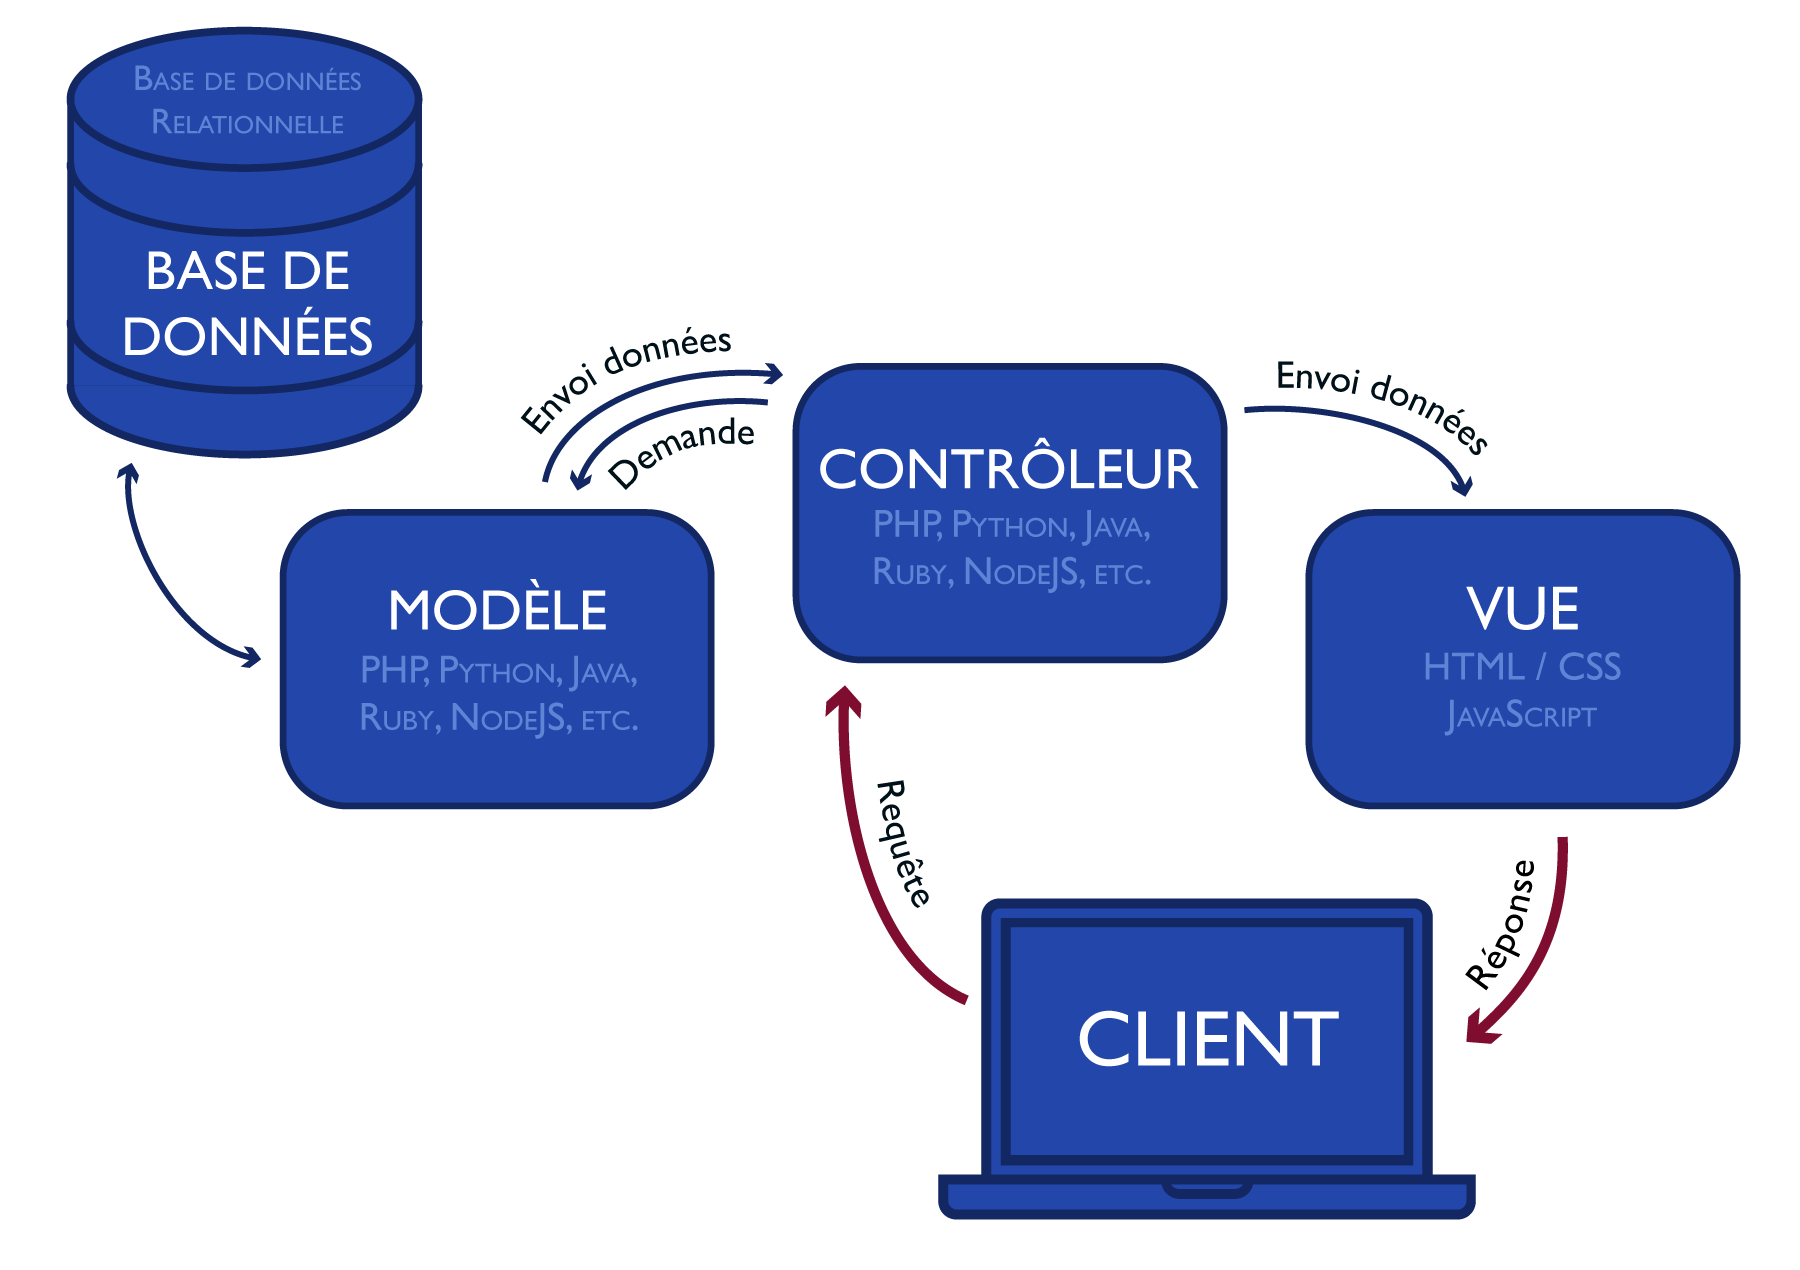
\includegraphics[width=14cm]{Images/Architecture-MVC.png}
	\caption{Fonctionnement simplifié de l'architecture logicielle \textsc{mvc}}
\end{figure}

			\subsubsection{Présentation du \emph{framework} Symfony}
L'application Web de \dishas a été élaborée grâce au \eng{framework} \mvc Symfony, dans sa version 3.4. Symfony est une infrastructure logicielle pour la création de sites internet en \php. Le langage de programmation \php est largement répandu dans le domaine du développement Web~; il est donc bien connu des directions de systèmes d'information, ce qui facilite la maintenance des projets utilisant ce langage. Il existe de multiples \eng{frameworks} \php et Symfony est l'un de ceux proposant le plus de fonctionnalités. Il est d'ailleurs le socle sur lequel se fondent d'autres \eng{frameworks} à l'instar de Laravel, lui aussi communément utilisé. Symfony compose un environnement de travail cohérent, utilisé pour de larges applications à l'instar de Dailymotion~; sa robustesse est également un atout pour les projets plus réduits comme \dishas, dans la mesure où il offre une grande fiabilité, en même temps qu'une importante adaptabilité. La documentation et la communauté soutenant cet outil en font un instrument robuste pour la conception d'une application Web ayant vocation à être pérenne.

				\paragraph{Structure de l'application}
L'arborescence des fichiers contenant le code nécessaire à l'exécution de l'application se divise en différentes branches, chacune chargée du fonctionnement d'un module précis. Il ne sera évoqué ici qu'un petit nombre de ces principaux composants.

Dans le dossier \eng{Entity} sont reproduites les tables de la \bdd~: pour chacune d'entre elles, une classe reprenant chacun des champs de la table est définie. Un enregistrement de la base sera ainsi transformé en objet \php utilisable dans le code~; à cet objet seront associées des méthodes spécifiques, afin de manipuler les propriétés qui lui sont associées. Pour récupérer le titre d'une entrée de la table \eng{Work}, on pourra par exemple employer la méthode \texttt{getTitle()}~; pour définir la valeur de la propriété \eng{title} de cet objet, on utilisera en revanche la méthode \texttt{setTitle()}. Le dossier \eng{Repository} quant à lui, définit pour chacune des entités des méthodes supplémentaires, davantage complexes, faisant jouer le rapport entre les données~; par exemple, l'entité \eng{Work} y dispose d'une méthode \texttt{getPrimarySources()} qui a pour but de récupérer toutes les sources primaires issues d'une œuvre.

Le dossier \eng{Controller} réunit quant à lui tous les contrôleurs, sortes de chefs d'orchestre de l'application. Les contrôleurs sont des fonctions qui agrègent les données nécessaires à la constitution d'une vue pour les transmettre au fichier de \eng{template}. Si l'on a par exemple besoin du titre et des sources primaires reliés à une œuvre au sein d'une page de l'interface, on stockera la valeur des deux méthodes évoquées précédemment à l'intérieur de variables~; ces variables seront ensuite ajoutées à la valeur de retour de la fonction, de manière à les faire parvenir aux fichiers de vues.

				\paragraph{Gestion des vues}
Le développement \eng{front end} –~portant sur ce que l'utilisateur voit à l'écran (utilisant notamment les langages \html, \css et JavaScript\footnote{De manière générale, le langage \html définit la structure d'une page Web, le \css son apparence graphique et JavaScript le comportement interactif des composants de la page.})~– concerne la partie \g{vue} de l'architecture \mvc. La conception des interfaces publiques de \dishas s'est donc concentrée en grande partie sur l'élaboration de \eng{templates} pour l'affichage des pages. Symfony dispose du moteur de \eng{templates} Twig, qui s'intègre directement dans le code d'une page \html. Twig sert notamment à transmettre les données définies dans la partie \g{modèle} de l'application au code qui sera envoyé au navigateur.

Pour afficher par exemple le titre d'une œuvre sur une page de notice, l'information contenue dans la \bdd doit d'abord être transposée en objet \php grâce au fichier d'entité définissant les caractéristiques d'une œuvre. L'information est ensuite récupérée par le contrôleur dédié aux pages de notices d'œuvre, puis transmise à la vue par le biais de Twig\footnote{Les passages Twig dans le \eng{template} \html sont repérables par leur balisage à l'aide d'accolades : \texttt{\{\{~~\dots~~\}\}}.}.

\begin{figure}[h!]
	\centering
	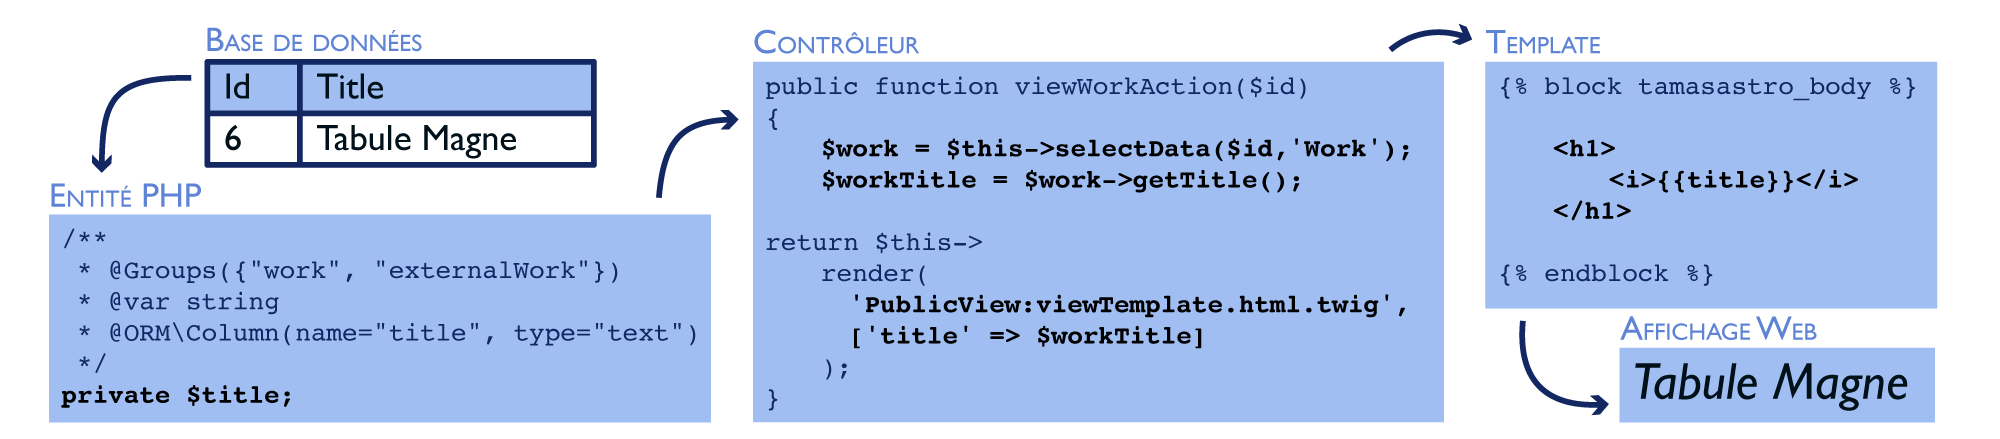
\includegraphics[width=16cm]{Images/Fonctionnement-mvc.png}
	\caption{Étapes pour l'affichage d'une donnée de la base au sein d'une page Web}
\end{figure}

%				\paragraph{Adaptabilité de l'application}
%Symfony est un \eng{framework} extrêmement configurable grâce au système de \eng{bundle}~: un \eng{bundle} est un répertoire qui permet d’implémenter une fonctionnalité à l'intérieur de l'application. Les fonctionnalités spécifiques à la plateforme \dishas sont d'ailleurs elles-même contenues dans un \eng{bundle} propre. On peut considérer que les \eng{bundles} sont une forme d'extension de Symfony. Il est par ailleurs possible de télécharger des \eng{bundles} conçus extérieurement au projet, ce qui permet de gagner du temps par rapport au développement de modules spécifiques, tout en fournissant une base de travail solide. Un des \eng{bundles} les plus importants de l'application \dishas est sans doute le \texttt{FOSUserBundle} qui s'occupe de la gestion des utilisateurs.

			\subsubsection{Stockage et récupération des données}
L'application de \dishas s'appuie sur une \bdd relationnelle~: cela signifie que les informations utilisées par la plateforme sont stockées à l'intérieur de tables, connectées entre elles par des relations définies à l'aide de cardinalités\footnote{La cardinalité désigne le nombre minimum et maximum de possibilités de relation entre deux entités. Par exemple, un \oi ne peut être contenu que dans une source primaire. Une source primaire en revanche peut contenir plusieurs \ois. La cardinalité entre ces deux entités est donc de 1 à n.}. Pour accéder aux données, l'application doit utiliser un intermédiaire logiciel que l'on nomme \orm. L'\orm de Symfony est appelé Doctrine~; il permet de faire le lien entre les tables de la \bdd et les classes du programme applicatif. Son rôle consiste donc à synchroniser les enregistrements de la base avec les objets \php de l'application.

Les fonctionnalités de Doctrine permettent d'interroger et récupérer de manière simple les données de la base. En convertissant en objets les données issues de la base relationnelle, l'\orm modifie la morphologie de l'information de manière à la rendre compatible avec la logique des langages orientés objet comme \php. Néanmoins, Doctrine constitue en cela une couche logicielle supplémentaire qui peut nuire aux performances générales de l'application.

		\subsection{Le paradigme client/serveur}
De nombreux systèmes informatiques reposent sur l'architecture client/serveur. Dans le cas des applications Web, elle désigne le mode de communication entre deux programmes~: le client est un programme qui envoie des requêtes et le serveur est un programme qui répond à ces requêtes. Dans une plateforme en ligne, le serveur est la machine qui envoie les pages apparaissant sur le navigateur de la machine client.

			\subsubsection{Distinction \eng{back end}/\eng{front end}}
Cette bipartition dans le fonctionnement de l'application fait écho à la distinction entre développement \eng{back end} et développement \eng{front end}. Le \eng{back end} fait référence à la partie du code –~rédigée en \php dans le cas de \dishas~– qui n'est pas visible à l'utilisateur. Le \eng{front end} en revanche représente la partie qui aura une influence directe sur ce qui est affiché sur l'écran du navigateur~: les langages utilisés dans le \eng{front} sont \html, \css et JavaScript.

Cette distinction se retrouve également dans la manière dont sont exécutés les différents langages utilisés dans la plateforme. L'intégralité du code écrit en \php est traité par le serveur, alors que le \html, \css et JavaScript sont interprétés par le navigateur sur l'ordinateur du client. Dans le cas des \eng{templates}, la partie Twig est exécutée par le serveur, tandis que le reste est à la charge de la machine client. Il existe ainsi différentes méthodes pour le traitement de la donnée~: une même information pourra manipulée et formattée à l'intérieur du \php, comme au sein du JavaScript.

Ces méthodes de traitement de la donnée ont chacune leurs implications. En premier lieu, la puissance de calcul du serveur est généralement plus importante que celle du client~; cela signifie que des procédures programmatiques lourdes sont effectuées plus rapidement si elles sont rédigées en \php. Il est ainsi préférable de circonscrire au maximum l'utilisation de JavaScript pour traiter les ressources numériques. Par exemple, si une interface a besoin d'un jeu de données formatté de manière spécifique, il est conseillé de le mettre en forme dans le \eng{back end}, plutôt que de transmettre des données brutes au \eng{front end} pour ensuite les agencer de manière adéquate. Ainsi, pour remplir le \eng{template} de barre latérale de métadonnées, une méthode propre à chaque entité a été définie dans les \eng{Repositories} afin de générer des tableaux associatifs\footnote{Un tableau associatif en \php est une manière d'organiser la donnée, où chaque valeur est associée à une clef. Ce format est comparable aux objets JavaScript ou aux dictionnaires Python. \newline Exemple~: \texttt{\$manuscrit = ["cote" => "Latin 14420", "folios" => 32, "langue" => "latin"]}.} contenant les métadonnées d'un enregistrement.

			\subsubsection{Contraintes du développement \eng{front}}
Toutefois, il n'est pas toujours possible de traiter les ressources numériques au sein du \eng{back end} de l'application. En effet, lors de l'utilisation d'ensembles de données importants au sein d'une même interface, il est parfois préférable d'avoir recours à des méthodes de programmation asynchrone\footnote{L'exécution du code est généralement linéaire, chaque ligne étant traitée l'une après l'autre. Dans le cas de l'asynchrone, la portion de code concernée est placée dans une file d'attente et n'est exécutée qu'une fois le reste du code effectué.} au sein du \eng{front end}, de façon à réduire les durées de chargement à l'ouverture de la pageß. En effet, JavaScript permet de récupérer certaines informations du serveur, sans entraver l'exécution du reste du code, de manière à éviter de soumettre l'utilisateur à d'importants temps d'attente.

Ce procédé est nommé \ajax~: le principe consiste à envoyer une requête au serveur, indépendamment du chargement de la page. Le code asynchrone est exécuté comme tâche de fond, sans occasionner de temps de latence lié à l'actualisation entière de la page. Cette technique est employée notamment pour charger de façon incrémentale un fil d'actualité, ou encore pour suggérer des termes d'autocomplétion dans un champ de saisie\footnote{La suggestion de termes se fondant sur une liste de mots accessible depuis une base distante.}~: cela permet de fluidifier la navigation, de manière à rendre transparent le processus de requêtage de données. La méthode \ajax est notamment employée dans le \fo pour récupérer les données nécessaires à la composition de la carte chronologique~: cette technique permet d'afficher certains éléments de la page avant que l'intégralité de la visualisation ne soit constituée.

Ces formes d'optimisation du code sont nécessaires à considérer dans le processus de développement des interfaces, en particulier pour les visualisations de données qui sont très coûteuses en termes de puissance de calcul. Le code \eng{front end} étant interprété par l'ordinateur du client, la rapidité d'exécution du programme dépend de la puissance de sa machine, ainsi que des capacités de compilation de son navigateur. S'il n'existe plus de sensibles différences entre les navigateurs Web, il subsiste quelques variations concernant certaines fonctionnalités implémentées par les langages \eng{front}.

La structure de l'application ainsi que l'architecture client/serveur conditionnent la manière dont est traitée l'information. Ainsi, pour assurer aux internautes une expérience de navigation agréable au sein du \fo, les problématiques de vitesse de chargement doivent influencer directement la manière dont sont pensés les développements. S'il est préférable d'effectuer la manipulation de données dans la partie \eng{back end} de la plateforme, il est cependant nécessaire de savoir repenser les méthodes de requêtage et de gestion des données, afin d'offrir aux utilisateurs des interfaces optimales et ergonomiques.

	\section{Implémentation d'ElasticSearch\label{Elastic}}
		\subsection{Présentation d'ElasticSearch}
			\subsubsection{Fonctionnement d'ElasticSearch}
ElasticSearch est un logiciel libre\footnote{ElasticSearch est un logiciel \eng{open source} sous licence libre Apache.} servant à l'indexation et la recherche de données~; il s'appuie sur une \bdd \nosql ainsi que sur le moteur de recherche Lucene\footnote{Lucene est un moteur de recherche modulable spécialisé dans la recherche textuelle}. Les bases de données \nosql se définissent en opposition aux bases relationnelles, elles recouvrent des formes aussi diverses que les bases graphes\footnote{Pour le stockage de triplets \rdf notamment.} ou les bases orientées documents\footnote{À l'instar des bases de données constituées de documents au format \xml ou \json.}. La base ElasticSearch s'organise autour d'un système complexe de \eng{clusters} et de nœuds très flexible, pouvant s'adapter à toute sorte de donnée. Ce type d'architecture a l'avantage d'être résilient, performant et de bien supporter la montée en charge. Les données insérées et récupérées de la base ElasticSearch sont au format \json, elles ne sont en revanche pas stockées ainsi.

La \bdd d'ElasticSearch est le support de son moteur de recherche. Les fonctionnalités proposées par ElasticSearch permettent à la fois d'y extraire un grand nombre de résultats à l'aide de requêtes imprécises, comme d'effectuer des recherches extrêmement détaillées, grâce à des possibilités de filtres extensives, tout cela avec une grande rapidité. Le moteur d'ElasticSearch est également fortement orienté texte, les résultats de recherche étant classés selon leur pertinence vis-à-vis des mots-clefs renseignés par l'utilisateur. La vitesse de requêtage ainsi que les fonctionnalités de recherche avancées sont deux atouts qui ont amené l'équipe technique de \dishas à implémenter cette solution en complément de l'\api. L'\api a vocation à servir principalement à interagir avec la \bdd relationnelle sans passer par l'interface graphique, tandis qu'ElasticSearch doit être utile à l'extraction d'importants ensembles de données et à la construction de requêtes complexes. ElasticSearch constitue en cela un élément essentiel de l'exposition des données de la base de \dishas.

L'implantation d'un serveur ElasticSearch est relativement aisée, la principale difficulté de l'implémentation de cet outil réside dans la constitution du \eng{mapping} définissant l'architecture conceptuelle de la base. Cette étape permet de transposer les données de la base relationnelle à l'intérieur de la base \nosql d'ElasticSearch~; elle a été facilitée par l'utilisation de l'extension Symfony FOSElasticaBundle. Certaines tables de la base n'ont pas été reproduites dans le \eng{mapping} d'ElasticSearch, seules les données intéressantes pour les chercheurs ont été intégrées.

			\subsubsection{Visualiser et explorer avec Kibana}
L'implantation d'ElasticSearch sur une base de données donne en outre accès aux différents outils de la suite Elastic. Kibana est l'un de ces outils~: il permet de créer par le biais d'une interface graphique des visualisations sur mesure, à partir des données indexées dans ElasticSearch. Les fonctionnalités de Kibana peuvent être étendues par l'ajout de \eng{plug-ins}, permettant l'utilisation de divers procédés d'analyse sur les données ainsi que de multiples types de visualisations. Certains des modules de Kibana sont par ailleurs payants, à l'instar de l'extension Graph développée par Elastic, qui permet de représenter les relations entre les enregistrements de la base sous forme de graphe.

Kibana a été originellement créé pour composer des tableaux de bord, aidant les administrateurs d'une application à visualiser les \eng{logs}\footnote{Les \eng{logs} sont des fichiers d'historiques des événements.}. S'il est possible de partager les visualisations réalisées avec Kibana et de les intégrer dans un fichier \html, elles ne sont pas conçues pour être diffusées sur une plateforme publique. Pour le projet \dishas, il a ainsi été décidé que l'accès à Kibana serait réservé aux chercheurs, de manière à leur permettre de créer des représentations graphiques sur mesure des données qu'ils souhaitent voir interagir.

		\subsection{Utilisation dans le \fo}
Les fonctionnalités de recherche proposées par ElasticSearch ont été largement utilisées au cours de l'élaboration des interfaces du \fo. La mise au jour des interactions entre les données étant au cœur de l'architecture de la plateforme publique, les modalités de recherche d'ElasticSearch ont permis de tisser des liens entre les ressources de manière plus efficace et précise que les méthodes de requêtage offertes par l'\orm Doctrine. ElasticSearch est ainsi utilisé à la fois dans la partie \eng{back end} de l'application, au sein du \php, mais également dans la partie \eng{front end} par le biais de méthodes de requêtage asynchrone.

			\subsubsection{Requêtage en \eng{back end}}
La barre latérale de métadonnées présente sur les pages d'enregistrements dispose d'un système de \g{loupes} qui rattache chaque notice aux enregistrements connexes de la base. Si une œuvre a par exemple été créée par Jean de Lignières, l'icône de loupe permet à l'utilisateur d'avoir accès à toutes les œuvres créées par le même auteur. Ainsi, pour chaque champ de la barre latérale est associée une requête à la \bdd correspondant à l'ensemble des entités partageant la même caractéristique.

Pour chaque entité de la base qui dispose d'une page de notice, a été définie une méthode spécifique permettant de générer les données à afficher dans cette barre latérale\footnote{Cette méthode est décrite plus en détail à l'annexe \ref{sidebar-of-metadata}.}. Cette méthode définit non seulement les métadonnées d'un enregistrement mais également les requêtes qui seront envoyées à ElasticSearch. Les requêtes faites à ElasticSearch sont formulées en \json, toutefois, cette technologie évolue rapidement et la syntaxe des requêtes est modifiée régulièrement. Afin d'aider à l'élaboration de ces requêtes et d'assurer une compatibilité accrue au cours du temps, il a été décidé d'utiliser le client \php Elastica qui permet faire le lien avec le serveur ElasticSearch dans le \eng{back end}. Elastica permet de formuler à l'aide d'une classe \php des requêtes qui seront ensuite traduites en \json.

Les requêtes à élaborer pour la constitution des barres de métadonnées conservent souvent des structures similaires et il aurait été redondant de reproduire systématiquement des procédures semblables pour chaque requête. Il a donc été décidé de créer une extension de la classe \texttt{Query} d'Elastica afin de systématiser la rédaction de requêtes.

Par exemple, voici la formulation d'une requête au format \json pour récupérer dans la base ElasticSearch tous les \oi élaborés entre 1450 et 1500, suivi de son équivalent, formulé à l'aide du client Elastica~:

\begin{figure}[H]
\begin{lstlisting}
GET original_text/_search
{
    "query": {
        "bool": {
            "must": [
                {
                    "range": {
                        "tpq_date": {"gte":"1450-01-01"}
                    }
                },{
                    "range": {
                        "taq_date": {"lte": "1500-01-01"}
                    }
                }
            ]
        }
    }
}
\end{lstlisting}
\caption{Formulation dans le langage de requête d'ElasticSearch}
\end{figure}

\begin{figure}[H]
\begin{lstlisting}
// Nouvelle instance de la classe Query
$query = new Elastica\Query();

// Création des filtres
$greaterThan = new \Elastica\Query\Range("tpq_date", ["gte" => "1450-01-01"]);
$lessThan = new \Elastica\Query\Range("taq_date", ["lte" => "1500-01-01"]);

$bool = new \Elastica\Query\BoolQuery();
$bool->addMust([$greaterThan, $lessThan]);

// Attribution de ces filtres à la requête
$query->setQuery($bool);
\end{lstlisting}
\caption{Formulation dans le langage de requête du client \textsc{php} Elastica}
\end{figure}

Avec l'extension de la classe \texttt{Query}, il est possible de créer la même requête en une ligne (\texttt{newTimeQuery(1450,1500)}) de manière à alléger le code et faciliter la maintenance. Ces requêtes sont ensuite insérées dans le tableau associatif servant à générer la barre latérale des pages de notices. Lors du clic sur une icône de loupe, la requête est envoyée à la page de recherche par le biais du contrôleur.

			\subsubsection{\label{Ajax-Elastic}Chargement asynchrone des données}
Le moteur de recherche ElasticSearch est employé pour deux utilisations distinctes dans la partie \eng{front end} de l'application~: pour la visualisation en carte ainsi que pour la page de recherche.

Toutes requêtes qui transitent par la page de recherche sont envoyées en \ajax à ElasticSearch. L'utilisation de méthodes asynchrones pour la récupération de résultats est particulièrement adaptée, dans la mesure où elles permettent d'effectuer plusieurs requêtes les unes à la suite des autres, sans nécessiter de réactualisation de la page.

%Les résultats de la requête envoyée depuis la page de notice pourraient en revanche être récupérés au sein du contrôleur, dans le \eng{back office}. Cependant, pour des questions d'homogénéité du le code, il a été décidé de traiter toutes les requêtes avec JavaScript.

\begin{figure}[h!]
	\centering
	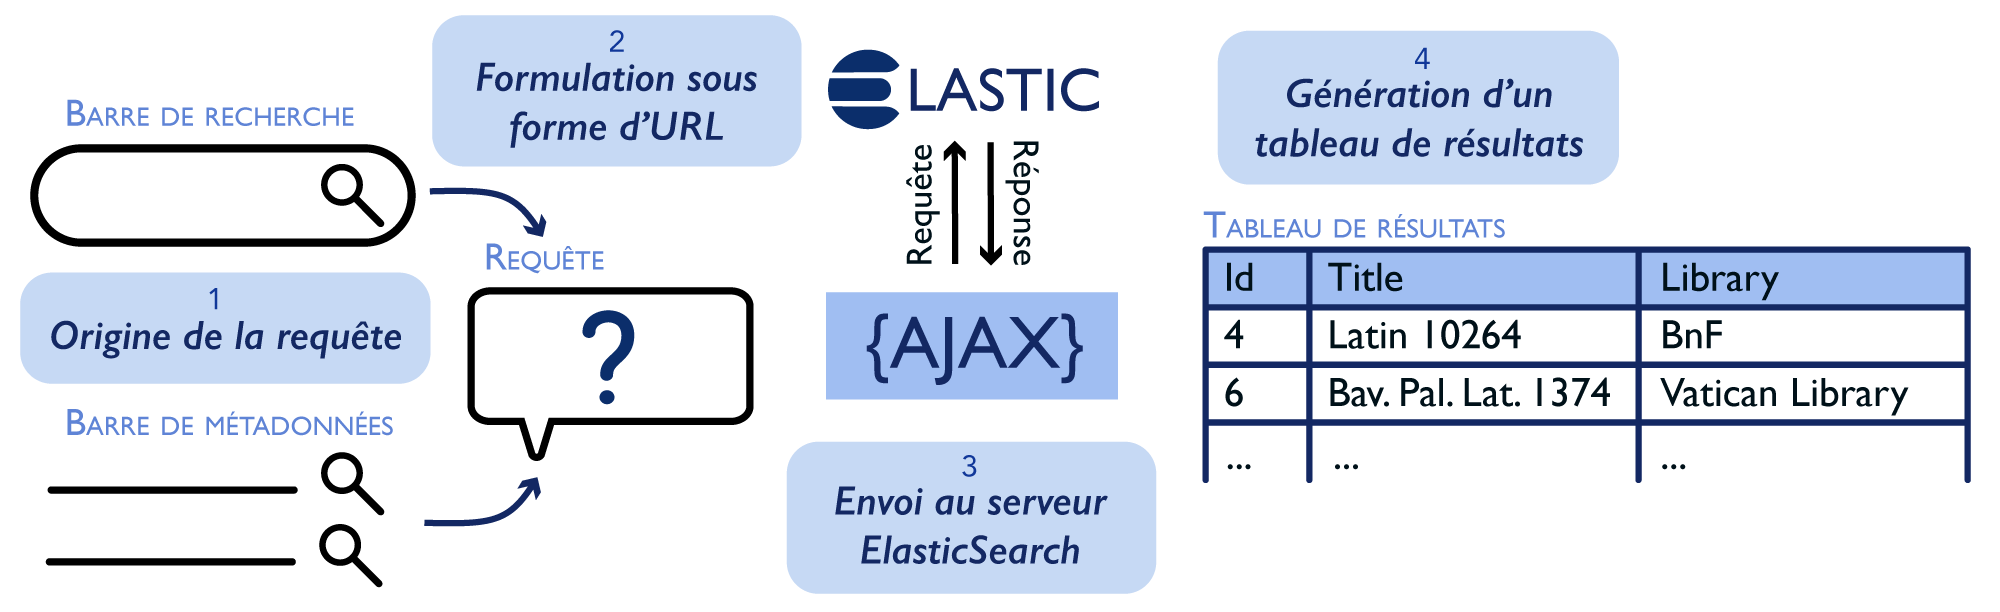
\includegraphics[width=16cm]{Images/Requete-Ajax.png}
	\caption{Processus de requête asynchrone à ElasticSearch pour la page de recherche}
\end{figure}

Le processus d'exécution d'une recherche suit toujours les mêmes étapes. Deux types de requêtes peuvent advenir~; soit la requête est envoyée depuis une page de notice, soit elle est formulée à partir des termes renseignés dans la barre de recherche. La requête est ensuite envoyée à ElasticSearch~; le résultat reçu est alors formaté de manière à apparaître au sein d'un tableau de résultats. Cette méthode permet de conserver un temps d'attente minimal pour la réception de résultat, tout en profitant des fonctionnalités avancées de recherche du moteur ElasticSearch. Cependant, seule la recherche plein-texte a été pour l'instant mise en place dans l'interface de recherche, il est prévu toutefois d'y ajouter la possibilité d'utiliser des filtres.

L'utilisation d'ElasticSearch pour la visualisation de carte chronologique répond à d'autres motivations. Cette visualisation en effet rassemble de nombreuses données, puisqu'elle vise à représenter tous les enregistrements d'œuvres et de sources primaires de la base. Le chargement de l'ensemble de ces données par l'intermédiaire de l'\orm Doctrine est supérieur à l'utilisation d'ElasticSearch. Il est toutefois difficile d'estimer exactement le gain de temps occasionné, dans la mesure où l'exécution du code asynchrone est postérieure au chargement de la page. De plus, la \bdd de \dishas reste pour l'instant assez réduite et les temps de requêtage restent courts. Néanmoins, pour la même quantité de résultats, le recours à ElasticSearch divise quasiment par deux le temps de chargement de la page (de 46,44~ms à 24,33~ms\footnote{Ces résultats ont été obtenus grâce au moniteur de performance de Symfony.}).\\

Ainsi, l'utilisation d'ElasticSearch est complémentaire au requêtage de la \bdd par un \orm~; si elle induit parfois la nécessité de traiter la donnée dans la partie \eng{front end} de l'application, elle offre des avantages de performance et participe à alléger les interfaces pour des visualisations plus fluides. ElasticSearch est également un outil indispensable pour explorer les données dans le détail, afin de permettre aux utilisateurs de réunir des données qu'il aurait été difficile de connecter en utilisant des langages de requêtes plus élémentaires\footnote{ElasticSearch permet notamment d'effectuer des recherches de distance par rapport à point particulier, par exemple pour retrancher tous les enregistrements créés dans un rayon de 100km. Reproduire le même résultat à l'aide d'un \orm ou du langage \sql est bien plus complexe.}.

\clearemptydoublepage

\chapter[De la conception à l'implémentation]{De la conception à l'implémentation des visualisations}
	\section{Technologies de visualisation de données}
		\subsection{Choix du moyen de réalisation}
Les visualisations de données sont une partie centrale de la plateforme publique~: elles constituent un moyen d'expression flexible et modulable pour exposer les données de recherche du projet \dishas. De nombreuses technologies numériques permettent de réaliser des visualisations, cependant elles ne sont pas toutes adaptées aux mêmes types d'application, et n'exigent pas le même niveaux de compétence en programmation.

			\subsubsection{Logiciels de visualisations}
Il existe une grande variété de logiciels permettant de composer des visualisations de données directement au sein d'une interface graphique. Ils n'exigent aucune connaissance préalable, si ce n'est une compréhension minimale des données à traiter. Les logiciels comme Excel, Tableau ou les plateformes comme Palladio et Kibana permettent à des utilisateurs novices de concevoir des visualisations riches et diversifiées. Néanmoins, les possibilités de configuration sont réduites aux fonctionnalités admises dans le logiciel, restreignant ainsi la variété des réalisations potentielles. En outre, ce genre d'outil n'est pas toujours adapté à la publication sur le Web~: s'il est souvent possible d'insérer ce type de visualisations à l'intérieur du code \html, il peut subsister des difficultés d'affichage. Dans le cas de Kibana notamment, l'intégration de visualisations à l'intérieur d'une page publique peut entraîner des failles de sécurité~; en ce qui concerne Tableau, toutes les réalisations sont conservées sur le serveur de l'application, occasionnant parfois des délais de chargement supplémentaires.

Les logiciels de visualisations sont particulièrement indiqués pour aider des chercheurs à concevoir des graphiques sur mesure~: pour des utilisateurs connaissant bien leur corpus de données, ces outils offrent des ressources intéressantes pour formuler graphiquement des hypothèses de recherche. En revanche, ces instruments ne sont souvent pas conçus pour être employés sur un site internet. Leur utilisation est à privilégier pour la création de visualisations ponctuelles, indépendantes d'une interface Web.

			\subsubsection{Visualisation de données avec R}
R est un langage de programmation statistique avec lequel il est possible de générer des visualisations de données. Il est extrêmement modulable et permet aux développeurs de créer une multitude de graphiques, grâce aux nombreuses extensions qui y être peuvent ajoutées. C'est un outil particulièrement employé dans le monde académique, notamment car il permet de manipuler les données à l'aide de fonctions statistiques et mathématiques avancées. Il est souvent utilisé en parallèle du langage de programmation Python, qui offre également des possibilités de visualisations et d'analyses statistiques extensives, grâce à des bibliothèques comme MatPlotLib ou encore Seaborn. Si R est plus généralement utilisé pour analyser des jeux de données en \textsc{csv}, il existe des \eng{packages} pour parser du \json, de l'\xml ou encore des fichiers de tableurs.

R n'est pas réputé pour être un langage difficile d'appréhension au premier abord, toutefois il semble que certains types de diagrammes nécessitent une connaissance accrue du langage pour être réalisés. En outre, R est plutôt dédié à la conception de graphiques statiques~; les bibliothèques additionnelles qui proposent d'ajouter de l'interactivité utilisent généralement JavaScript pour les éléments dynamiques\footnote{Notamment pour bibliothèques Plotly, DT et Shiny qui intègrent toutes des fonctionnalités d'interactivité à l'aide de JavaScript.}.

			\subsubsection{Bibliothèques JavaScript}
En ce sens, il semble plus indiqué de n'avoir recours qu'à JavaScript pour créer les visualisations de données dans le \fo. Il existe un grand nombre de bibliothèques JavaScript spécialement dédiées à l'intégration de visualisations de données aux pages Web. Ces bibliothèques disposent toutes de spécificités~; certaines sont extrêmement versatiles et polyvalentes –~à l'instar de D3.js ou Chart.js\footnote{D3.js et Charts.js sont à la tête du marché des visualisations sur le Web d'après \ref{WappalyzerJavaScriptGraphics2019}.}~– tandis que d'autres sont spécialisées dans un unique type de graphique –~comme Leaflet pour les cartes ou Chartist pour les diagrammes simples. La richesse d'une bibliothèque JavaScript est souvent corrélée à la difficulté de son apprentissage~; en outre, plus les visualisations à réaliser sont complexes, plus une connaissance approfondie de la bibliothèque est nécessaire.

Il existe des bibliothèques JavaScript adaptées à tous les usages~; si cette richesse est profitable, elle rend le choix d'une technologie particulièrement ardu. Plusieurs questions sont donc à considérer~: quels types de visualisations sont prévus~? Quelle est la taille du jeu de données à traiter~? Quel environnement de développement est utilisé au sein du projet\footnote{L'emploi de \eng{frameworks} comme React ou Angular peuvent conditionner le choix vers des bibliothèques compatibles.}~? L'application doit-elle être disponible en version mobile~? Les fonctionnalités de la bibliothèque sont-elles bien supportées par les différents navigateurs~? Quel degré de personnalisation de l'interface est nécessaire~? Chacune des réponses à ces interrogations conditionne le choix d'une bibliothèque.

		\subsection{Choix d'une bibliothèque JavaScript}
			\subsubsection{Critères de choix}
Ainsi, le choix d'une bibliothèque JavaScript doit prendre en compte de nombreux paramètres. En premier lieu, le régime de tarification est important à considérer~: en effet, le projet \dishas ne bénéficie pas de financements suffisants pour payer la licence d'une bibliothèque JavaScript~; or, si la plupart proposent une partie de leurs fonctionnalités gratuitement, il existe souvent certaines conditions d'utilisation payantes. Il faut donc veiller à sélectionner une bibliothèque qui accepte les usages prévus pour le \fo de la plateforme.

Un second critère essentiel de choix concerne la documentation et la communauté liées à une technologie. En effet, une bibliothèque extrêmement efficace et flexible ne peut être utilisée au maximum de son potentiel, s'il n'existe pas d'exemple ou de documentation auxquels se référer pour l'utiliser. La communauté de développeurs peut également être de grand secours~; une question relative à une bibliothèque largement utilisée sera résolue très rapidement sur des sites comme StackOverflow. Un bon indicateur de la vivacité d'une communauté peut être trouvé sur les \eng{repositories} GitHub des différentes technologies~: le nombres d'étoiles\footnote{Les étoiles indiquent sur GitHub le nombre d'utilisateurs ayant mis en favori un projet en particulier.} et la date du dernier \eng{commit} peuvent être ainsi révélateurs du dynamisme d'un projet.

Un autre élément à considérer est évidemment les fonctionnalités offertes par une bibliothèque. La recherche de technologies de visualisations de données s'est fait ultérieurement à l'élaboration des graphiques à implémenter dans le \fo~: ainsi, il était important que la bibliothèque choisie comporte une grande variété de visualisations, notamment des visualisations en carte. La flexibilité de la bibliothèque est particulièrement importante dans la mesure où \dishas est un projet aux effectifs réduits et que l'utilisation de grand nombre de dépendances augmente la difficulté à maintenir l'application. En outre, la partie \eng{back office} de la plateforme disposait déjà de visualisations~; le choix d'une technologie s'est donc fait de manière à complémenter les bibliothèques préalablement implémentées dans l'application.

La bibliothèque de visualisations pour \dishas devait donc être à la fois robuste, versatile et fortement personnalisable. Une première sélection de bibliothèques a donc été effectuée en fonction des critères énoncés ci-dessus pour être mise à l'épreuve. Cinq bibliothèques\footnote{Il s'agit des bibliothèques Chart.js, D3.js, Google graphs, ApexCharts et AmCharts.} ont été testées dans la réalisation du graphique envisagé pour la notice d'œuvre~: il s'agit d'un graphique en colonnes relativement simple, idéal pour une première évaluation des possibilités d'une bibliothèque. Cette expérimentation a permis de déceler certaines différences de modélisations des données, ainsi que les avantages et inconvénients de ces technologies. Par exemple, D3.js est une bibliothèque remarquablement développée, ce qui rend sa première appréhension particulièrement difficile. Par ailleurs, Chart.js s'appuie sur l'élément \html \texttt{canvas}, là où les autres bibliothèques emploient l'élément \texttt{svg}~: cette différence a une influence sur la rapidité de chargement d'une visualisation. En effet, les bibliothèques utilisant le format \svg offrent davantage de flexibilité, car chaque élément du graphique correspond à un nœud unique du \dom\footnote{Le \dom correspond à l'architecture en arbre d'un document \html.} qu'il est possible de configurer. En revanche cela signifie également que plus nombreuses seront les données à afficher, plus le temps de chargement sera important~; l'élément \texttt{canvas} \eng{a contrario} est traité comme un assemblage de pixel par le navigateur, et donc est comparable à une simple image en termes de chargement.

			\subsubsection{Présentation de AmCharts}
La bibliothèque AmCharts a finalement été retenue pour le développement des interfaces publiques, en premier lieu pour la variété des visualisations qu'elle propose~: AmCharts offre plus de quinze types de graphiques différents, comprenant notamment des cartes, alors que ces dernières font généralement l'objet de bibliothèques spécialisées. Amcharts est une bibliothèque utilisée par de grandes entreprises, comme Amazon, Apple ou la \textsc{nasa}~; cela garantit la fiabilité de cette technologie, ce qui est important pour un projet comme \dishas. Son utilisation est gratuite à condition de conserver le logo d'AmCharts dans le coin inférieur des visualisations de données.

\begin{figure}[h!]
	\centering
	
\includegraphics[width=8cm]{Images/AmCharts.png}
	\caption{Logo de la bibliothèque JavaScript AmCharts}
\end{figure}

Amcharts dispose en outre d'une impressionnante documentation et de très nombreux exemples de visualisations, ce à quoi s'ajoute un blog où sont régulièrement postées des astuces pour la confection de graphiques complexes et modulables. Un avantage de cette bibliothèque réside dans la possibilité de configurer tous les éléments d'une visualisation, de manière à s'adapter au plus près des envies des concepteurs. Elle propose par ailleurs de nombreuses fonctionnalités pour concevoir des visualisations interactives et dynamiques, que l'utilisateur peut manipuler. Pour une première approche de la bibliothèque Amcharts, un tutoriel succinct a été mis à disposition à l'annexe \ref{AmCharts}~; des fichiers \html simplifiés, reproduisant les visualisations déployées dans le \fo, ont été également ajoutés aux appendices documentaires du mémoire.

	\section{Constitution d'une visualisation}
		\subsection{Dialogue entre conception et réalisation}
La constitution d'une visualisation consiste souvent en un travail itératif, où phases d'élaboration et de développement se répètent jusqu'à obtenir à une forme graphique satisfaisante. La visualisation permet de révéler des informations sur les données qui n'étaient pas prises en compte au départ, donnant lieu parfois à des incohérences ou des incompatibilités graphiques~; il est donc souvent nécessaire d'effectuer de multiples aller-retours entre réflexion et réalisation, pour parvenir à la visualisation la plus pertinente.

Le diagramme en barre prévu initialement pour la page de notice ds sources primaires a particulièrement évolué entre sa forme liminaire et son aspect final. Cette visualisation a initialement été conçue en miroir de la notice d'œuvres~: l'enjeu était d'y représenter chaque \oi contenu dans une source primaire, classé en fonction de l'œuvre dont il est tiré. À la suite de discussions avec les chercheurs du projet au cours d'un séminaire \dhu, il a été décidé d'intégrer une composante de foliotation au graphique, pour proposer deux modes de visualisation~: un présentant la quantité d'\ois par œuvre et un autre montrant leur disposition au sein de la source primaire. Une seconde version de la visualisation a donc été réalisée~; il est alors apparu que plusieurs \ois pouvaient être accolés les uns aux autres sur une même page. Sur la visualisation, les éléments représentant les \ois étaient ainsi superposés les uns sur les autres sans qu'il soit possible de les distinguer. Une seconde étape de programmation a donc été mise en œuvre, pour faire en sorte de distinguer les items situés sur les mêmes folios.

\begin{figure}[h!]
	\centering
	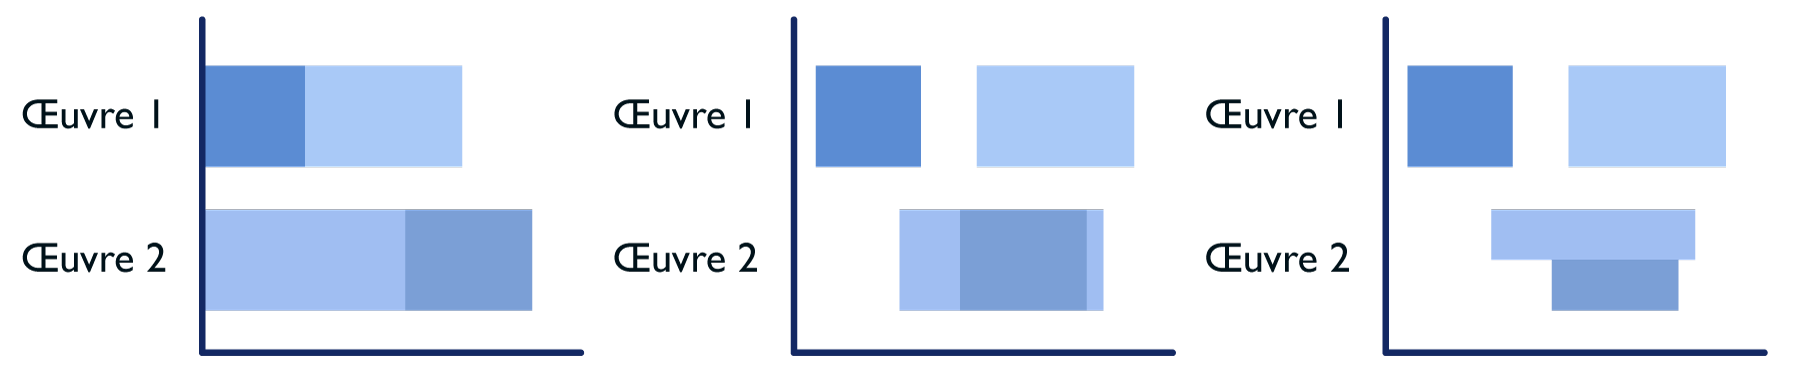
\includegraphics[width=15cm]{Images/Evolution-visualisation.png}
	\caption{Évolution de la visualisation pour la page de notice de sources primaires}
\end{figure}

C'est alors sur la visualisation représentant la quantité accumulée de folios –~montrant les \oi juxtaposés les uns aux autres~– que se sont portées les réflexions~: n'est-il pas trompeur de figurer comme étant un nombre total de folios, ce qui est en réalité l'accumulation des folios de chaque \oi pris indépendamment~? En effet, cette configuration peut donner l'impression qu'une œuvre compose la majeure partie d'une source primaire, alors qu'elle comptabilise moins de pages qu'une autre. Plusieurs solutions ont été envisagées pour pallier à cet effet~: ne représenter par exemple que le pourcentage d'\oi par œuvre, ou encore signifier par différentes épaisseurs la proportion prise par l'item au sein du folio. Il a finalement été décidé de conserver une visualisation avec des \ois accolés les uns aux autres\footnote{En plus d'une visualisation des \ois répartis tels que dans la source primaire.}, car elle permet d'évaluer la quantité de tables issues de chaque œuvre, ce qui est aussi significatif qu'un nombre de folios. En outre, un diagramme circulaire a été ajouté au sein de la barre latérale afin de représenter la part véritable de chaque œuvre au sein d'une source. Il reste cependant des interrogations vis-à-vis de cette visualisation, notamment la question du mélange entre folio et page (dans le cas de manuscrits recomposés) qui a pour l'instant été éludée\footnote{Il semble qu'une telle configuration sera rarement rencontrée~; pour l'instant, les deux systèmes de pagination sont traités de manière quasi équivalente.}.

		\subsection{Anticiper les obstacles à la visualisation}
Il existe donc de nombreux paramètres qu'il n'est pas toujours possible de connaître préalablement, mais qu'il faut essayer de prendre en compte, pour assurer l'adéquation de la représentation graphique avec la donnée à figurer. La \bdd sur laquelle s'est appuyée le travail d'élaboration des interfaces est encore profondément lacunaire, et comporte de plus de nombreuses données de test, n'ayant aucune véracité scientifique~; en outre, si la base ne sera ensuite alimentée qu'avec des données contrôlées, il subsistera inévitablement des variations dans la description des enregistrements. Toutes ces composantes sont à anticiper pour proposer des visualisations flexibles, susceptibles de conserver leur pertinence, malgré une incertitude vis-à-vis de la donnée.

			\subsubsection{Données lacunaires}
Le premier élément auquel une interface modulable doit faire face est l'inconsistance des données. L'absence d'une donnée peut être envisagée de deux manières différentes dans une visualisation~: soit ne pas faire figurer l'information manquante, soit la représenter, mais en la distinguant des autres. Dans les pages de notice, il est fréquent qu'un enregistrement ne dispose pas de toutes les métadonnées qui puissent lui être associées~; il est important de discerner parmi les informations qui font défaut, celles qui sont signifiantes, de celles accessoires. Par exemple, au sein de la barre de métadonnées, certains champs sont éludés s'ils ne sont pas renseignés, alors que d'autres sont conservés pour souligner l'absence de l'information\footnote{Ce point est discuté en détail en annexes \ref{managing-missing-information}.}. Par ailleurs, cette absence peut être le signe que l'information n'a simplement pas été renseignée par l'administrateur, ou qu'il n'est pas possible de la donner dans la mesure où le document originel ne permet pas de statuer. Ainsi, l'absence de donnée est un point délicat qu'il n'est pas possible de résumer aisément au sein d'une visualisation~; chaque métadonnée doit être traitée différemment.

Les visualisations de données de la plateforme publique servent, dans la plupart des cas, de portails vers les autres pages de l'interface publique~: la carte chronologique par exemple est le seul moyen d'accès –~mis à part l'interface de recherche~– aux notices d'œuvres et de sources primaires. Chacune de ces entités doit donc figurer sur la carte, quand bien même elle ne serait pas associée à un lieu en particulier. Ainsi, toutes les données qui ne sont pas situées géographiquement ont été arbitrairement placées aux coordonnées 0,0.

De la même manière, il n'est pas exigé dans le modèle de données de préciser les pages d'un \oi, ce qui met en cause la visualisation de la notice de sources primaires. Pour remédier à ce problème, il a été décidé d'obliger les utilisateurs à remplir ce champ au moment de la soumission du formulaire pour l'insertion d'un nouvel item. Des valeurs par défaut peuvent être renseignées si l'information est véritablement manquante. Il s'agit d'inciter les chercheurs à décrire le plus exhaustivement les données qu'ils ajoutent à la base~; en revanche, il ne faut pas que les visualisations prévalent sur l'exigence scientifique. C'est pourquoi chacune de ces décisions doit être attentivement évaluée en compagnie de l'équipe de recherche, de manière à encourager l'utilisation de la plateforme en proposant des visualisations éclairantes, mais en contraignant le moins possible la pratique des chercheurs.

			\subsubsection{Données trop abondantes}
Si les données lacunaires peuvent poser problème, l'abondance des données peut également susciter des difficultés. La superposition des éléments graphiques et la concentration des informations peuvent en effet rendre illisible une visualisation. Certaines fonctionnalités et formes visuelles cependant permettent d'éviter ces écueils, en atténuant la complexité des données~; les cartes proportionnelles (\eng{treemap}) et les diagrammes circulaires notamment, figurent de manière facilement appréhendable de grandes diversités d'information en minimisant la part des données en faible proportion. Les modalités de zoom donnent également l'occasion à l'utilisateur de cadrer la visualisation à l'échelle qu'il trouve la plus cohérente.

Cependant, la principale difficulté de l'abondance de données à visualiser est avant tout la lenteur de chargement qui peut en être occasionnée. L'utilisation d'une bibliothèque JavaScript pour réaliser les cartes et les diagrammes du \fo induit que le code sera exécuté sur l'ordinateur du client~: la puissance de la machine et l'efficacité du navigateur étant inconnus, il est nécessaire d'alléger au maximum la partie programmatique du \eng{front end}. Les méthodes de chargement asynchrone ou incrémental (\eng{lazy loading}) permettent notamment de répartir les passages les plus coûteux en puissance de calcul, en échelonnant le chargement des composants à afficher. Il faut en effet distinguer la vitesse de chargement d'une page Web, de sa vitesse d'affichage~: la première est une mesure technique, tandis que la seconde est liée à la perception de l'utilisateur. Une page peut être affichée rapidement sans que son chargement soit terminé, offrant ainsi une expérience utilisateur jugée satisfaisante\footnote{La vitesse d'affichage est par ailleurs prise en compte dans le système de classement des moteurs de recherche.}. D'autres procédés ont vocation a être intégrés au \fo pour fluidifier encore davantage la vitesse d'exécution des scripts, notamment le regroupement des données en \eng{clusters}, moins coûteux à traiter par le navigateur. Toutefois, les ajustements programmatiques qui ont été implémentés pour l'instant restent limités, du fait de mes compétences techniques encore modestes.

Pour évaluer les performances des pages publiques, le \eng{bundle} de Symfony appelé Fixtures a été utilisé. Cette extension permet d'ajouter de grandes quantités de données à la base, afin de tester la réaction des interfaces. La carte chronologique a été le principal objet de cette évaluation, dans la mesure où il s'agit de la visualisation agrégeant le plus de données~: cela a permis d'identifier certains points à simplifier\footnote{Le niveau de description de la carte de chaleur en particulier, de manière à passer d'une granularité à l'année à des tranches temporelles d'une décennie.}, mais également de ne constater aucun problème majeur. Les navigateurs en outre, disposent d'outils intégrés permettant d'estimer les passages du code exigeant le plus de performance, rendant ainsi possible de caractériser les passages du script à améliorer.

L'efficacité et la vitesse d'affichage des pages publiques de \dishas ne constitue pas uniquement des ajustements superficiels~; ces éléments sont d'une importance capitale si l'on veut inciter les chercheurs à utiliser les outils de la plateforme. L'augmentation de la performance des navigateurs a engendré un nouveau paradigme pour le développement d'applications~; ce qui pouvait être téléchargé et installé est aujourd'hui plus volontiers en ligne, accessible sur n'importe quel poste d'ordinateur. Les applications en ligne deviennent de plus en plus sophistiquées, habituant ainsi les utilisateurs à des interfaces complexes, chargeant de manière quasi instantanée. Si le \fo de \dishas n'offre que des outils laborieux à manipuler, les utilisateurs seront d'autant plus prompts à se désintéresser de la plateforme. La vitesse d'un site Web participe donc à l'exposition des données et doit être prise en considération, au même titre que l'ergonomie générale des interfaces.\\

Que ce soit pour gérer l'abondance ou l'insuffisance des données, la flexibilité des visualisations aide à manier des ressources dont la forme est imprévisible. Le modèle de données induit un nombre fini de possibilités concernant le format des enregistrements de la base~; le rôle du concepteur des interfaces est de veiller à trouver un mode d'affichage pour chacune de ces éventualités, de manière à prévenir les incompatibilités techniques ainsi que les aberrations graphiques. Dans la mesure où la structure de la \bdd est encore amenée à évoluer, il sera néanmoins nécessaire de revoir l'agencement des pages du \fo\footnote{Notamment pour l'aspect \eng{responsive} des interfaces, dimension qui n'a pas été encore abordée au sein de la plateforme \dishas.}, même si la structure de la plateforme publique a été pensée pour admettre des évolutions.

		\subsection{Limites de la visualisation}
S'il est un moyen d'appréhender aisément des informations complexes, le format graphique qu'offrent les visualisations de données peut également induire en erreur. Parfois la donnée en elle-même est ambiguë et il n'existe pas de forme visuelle adaptée~; parfois la représentation graphique véhicule des concepts qui ne sont pas en adéquation avec le contenu.

			\subsubsection{Incertitude relative à la donnée}
Le premier élément pouvant aboutir à une visualisation trompeuse est relatif à la forme des données sur lesquelles elle s'appuie~: qu'il s'agisse de l'aspect lacunaire de certaines informations ou de l'accumulation des données, il existe de nombreux prédicats qui peuvent biaiser une visualisation dans son ensemble. Par ailleurs, plus une visualisation résume une importante quantité de données, plus elle est susceptible de transmettre une impression d'exhaustivité~; cependant, la \bdd ne reflètera jamais que les documents sur lesquels des chercheurs ont porté leur attention. Le contexte de présentation d'une visualisation peut aider à dissiper cette équivoque, en faisant en sorte d'exposer les données en tant qu'enregistrement d'une base, et non comme représentation objective de la réalité historique.

Si les visualisations de notices ont une dimension plus exacte du fait de leur ponctualité, il subsiste des incertitudes quant à la représentation de certaines données. Dans le cas par exemple d'une source primaire qui mêlerait deux types de pagination –~folio et page~– essayer de représenter les deux formes de contenu sur la même échelle\footnote{En convertissant les folios en pages par exemple.} serait fautif~: en effet, ce genre de configuration est généralement signe d'un ouvrage hétérogène composé de parties indépendantes. Faire figurer côte à côte ces différentes parties est donc souvent erroné. Il n'est pourtant pas possible de présumer de la disposition des feuillets d'un ouvrage, en conséquence, une visualisation de données générique ne pourra jamais être tout à fait adéquate. L'idéal serait de pouvoir s'appuyer sur la pagination d'une reproduction numérique, il n'existe cependant pas de numérisation de tous les documents à intégrer à la base, rendant le travail de conception des interfaces d'autant plus délicat.

			\subsubsection{Représentations biaisées}
La seconde difficulté dans l'élaboration d'une visualisation pertinente réside dans l'aspect graphique à choisir pour représenter la donnée. L'échelle, la couleur, la forme ou encore l'interaction des différents éléments, véhiculent des informations à l'utilisateur. Chacun de ces composant doit être choisit avec soin, car il influence l'appréciation des données présentées. Par exemple, la simple flucutuation de l'échelle peut induire des conclusions tout à fait constrastées sur une même donnée~; une graduation resserrée amplifie les phénomènes de variation, l'inverse les atténue.

\begin{figure}[h!]
	\centering
	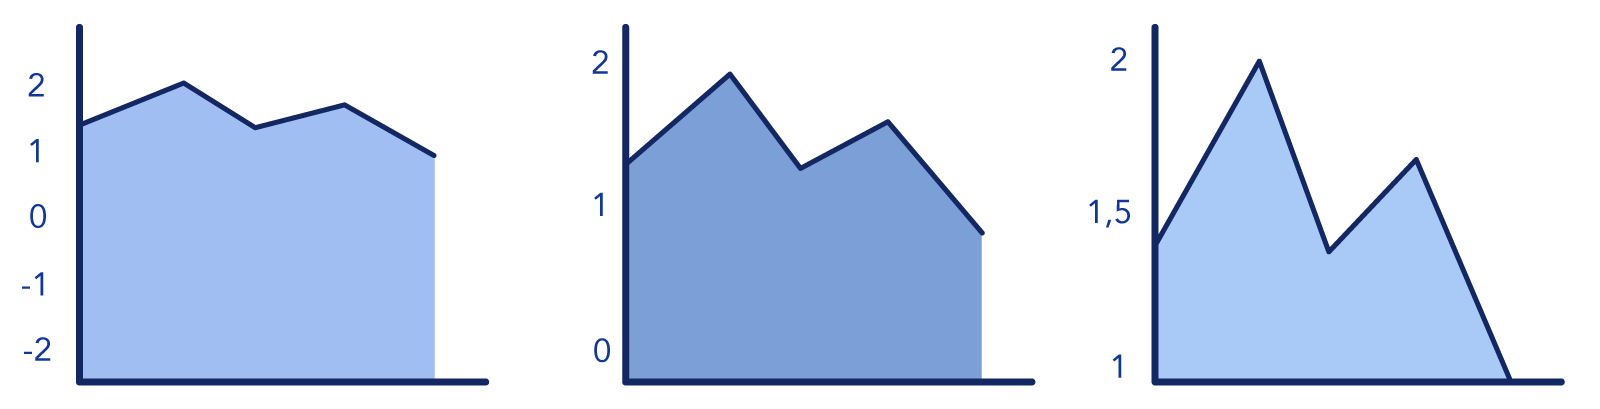
\includegraphics[width=15cm]{Images/Echelle-visualisation.png}
	\caption{Conséquences visuelles du changement d'échelle d'une visualisation}
\end{figure}

Au sein du \fo, plusieurs visualisations ont soulevé des questionnements relatifs à la représentation idéale des informations. Par exemple, comment figurer le chevauchement des \ois au sein d'une même page~: par transparence~? par un système de rayures colorées~? Il a finalement été décidé de superposer horizontalement les blocs d'\oi de manière à pouvoir cliquer indépendamment dessus. Néanmoins, il existe de multiples manières d'exprimer visuellement cette information~; le concepteur des interfaces doit s'efforcer de trouver celle qui est la plus adaptée, tout en restant réalisable.

La visualisation de la page de navigation historique a également été problématique~: si l'utilisation d'une carte a semblé évident, le choix d'un mode de représentation de la temporalité a été l'objet d'interrogations. La frise chronologique devait faire figurer la quantité d'œuvres et de sources primaires créées par période~; dans un premier temps, un diagramme linéaire a été choisi. Cependant, les dates de création encodées dans la base indiquent en réalité une période de conception probable~: une œuvre conçue entre 1400 et 1450 correspond sur un diagramme linéaire, à un plateau d'un demi siècle. Or, l'utilisateur peut comprendre de cette mise en forme qu'une œuvre a été créée toutes les années entre 1400 et 1450, ce qui est contradictoire avec la donnée de départ. C'est pourquoi, il a été jugé préférable de suggérer ces variations grâce à une carte de chaleur, où la saturation retranscrit plus justement la fluctuation dans le rythme de production.\\

Chacun des aspects d'une visualisation, dans la mesure où il peut être vecteur de renseignement sur la donnée, doit être choisi avec soin. Depuis le choix d'une technologie pour réaliser des diagrammes, jusqu'à la formulation des libellés, l'élaboration de visualisation mobilise de multiples modalités de médiation, à chaque étape de son processus. De plus, les données de recherche induisent un degré d'exigence scientifique supplémentaire à la conception de graphiques pour les représenter~: l'élaboration des pages de la plateforme publique de \dishas a ainsi tenté de valoriser aux mieux les ressources numériques par différents d'expression, autant visuel que conceptuel.

\clearemptydoublepage

\mychapter{Conclusion}
\addcontentsline{toc}{chapter}{Conclusion}
Ce mémoire s'est attaché à décrire le travail réalisé au cours du stage que j'ai effectué au sein de l'équipe de recherche de \dishas, à l'Observatoire de Paris. La mission qui m'avait été confiée consistait en l'élaboration de l'interface publique de l'application Web du projet~: il était important pour l'équipe de \dishas de disposer d'une plateforme ouverte, qui participe à valoriser les données produites dans le cadre du projet, tout en restant accessible à des publics variés. Les réflexions qui ont accompagné mon travail se sont concentrées sur les différentes modalités de médiation numérique par lesquelles il est possible de présenter un corpus de recherche. Mes réalisations se sont attachées à fournir des solutions à chaque étape de conception de la plateforme, tant au niveau du parcours de navigation, que de l'interactivité des interfaces ou encore de l'agencement des visualisations de données.\\

Le processus de création de la plateforme publique du projet \dishas s'est déroulé en plusieurs phases successives. Une première phase d'analyse du contexte a permis d'appréhender le cadre dans lequel s'inscrivait ce travail. Une seconde phase de réflexion a été consacrée aux différents modes de médiation qu'il est possible d'appliquer à un corpus de données scientifiques. Enfin, une phase de réalisation technique a été l'occasion de développer certaines des interfaces de la plateforme.\\

La première partie de ce mémoire porte donc sur le contexte de création des données à valoriser, de manière à mieux appréhender les besoins qui peuvent émaner de la nature de ces ressources. La variété des approches scientifiques des équipes associées au projet permet notamment de comprendre la diversité des modes d'utilisation du matériel documentaire~: il est ainsi possible d'en déduire des exigences vis-à-vis des instruments informatiques à développer. La nature du corpus et les procédés de sa numérisation constituent également des axes de réflexion privilégiés, car la \bdd compose véritablement le socle sur lequel peut se construire la plateforme en ligne.

En second lieu se pose la question de la mise en forme de ces données. Dans cette optique, trois modes de médiation des ressources numériques ont été établis comme objectif de l'interface publique~: la présentation du corpus, l'accompagnement du travail de recherche et l'exposition des données brutes. La présentation des ressources numériques vise à les rendre explicites tout en introduisant les utilisateurs aux enjeux scientifiques qui sous-tendent le projet. L'accompagnement du travail de recherche consiste quant à lui à fournir des instruments pour assister les chercheurs dans leurs investigations du corpus numérique. L'exposition des données brutes enfin, a pour ambition d'aider ceux qui voudraient exploiter ces ressources~: elle vise à rendre accessible non seulement les données, mais également la documentation qui leur est associée.

Enfin, la description technique des différents composants de l'interface publique permet d'exposer les moyens mis en œuvre pour réaliser cette médiation de données. Ces instruments comprennent à la fois des infrastructures logicielles fiables, permettant d'assurer le fonctionnement global de la plateforme, mais aussi des modes de stockage et requêtage alternatifs de la donnée, ou encore le recours à des bibliothèques \eng{front end}, pour la création d'interfaces sur mesure. Par ailleurs, le travail technique réside également dans l'établissement de bonnes pratiques, à la fois pour la gestion des développements programmatiques, mais également pour assurer le dialogue entre recherche et ingénierie.\\

Au sein de la conception de la plateforme publique, le travail de médiation consiste donc à dresser une passerelle entre la \bdd et l'utilisateur, en mobilisant à la fois une appréhension fine du corpus de recherche, une compréhension des attentes des différents publics ainsi que des connaissances des technologies numériques. L'interface publique doit proposer un discours sur la donnée qui réponde à des questions de recherche, en mettant en œuvre différents principes de médiation à l'aide de procédés informatiques. La plateforme de \dishas vise à exposer la donnée de manière conforme aux principes \fair, de manière à participer à un écosystème ayant pour but la valorisation des ressources numériques.\\

L'élaboration des interfaces du \fo n'est cependant pas achevée et il subsiste encore de nombreuses formes d'expression la donnée à explorer. Le projet \dishas n'en est par ailleurs qu'à son commencement et il n'est pas encore possible d'évaluer avec précision l'adéquation des développements avec la pratique des utilisateurs. Ainsi, de nombreuses perspectives se dessinent quant à l'évolution des modes de valorisation du corpus de recherche~; l'accroissement de la base de données va être notamment la première étape vers la constitution de contenus inédits, en particulier car elle va être l'occasion de voir émerger de nouvelles hypothèses de recherche.

\appendix
	\part*{Annexes}	
	\addcontentsline{toc}{part}{Annexes}
	
	\chapter{\label{BaseDeDonnee}Base de données du projet}
	\begin{sidewaysfigure}[h!]
		\centering
		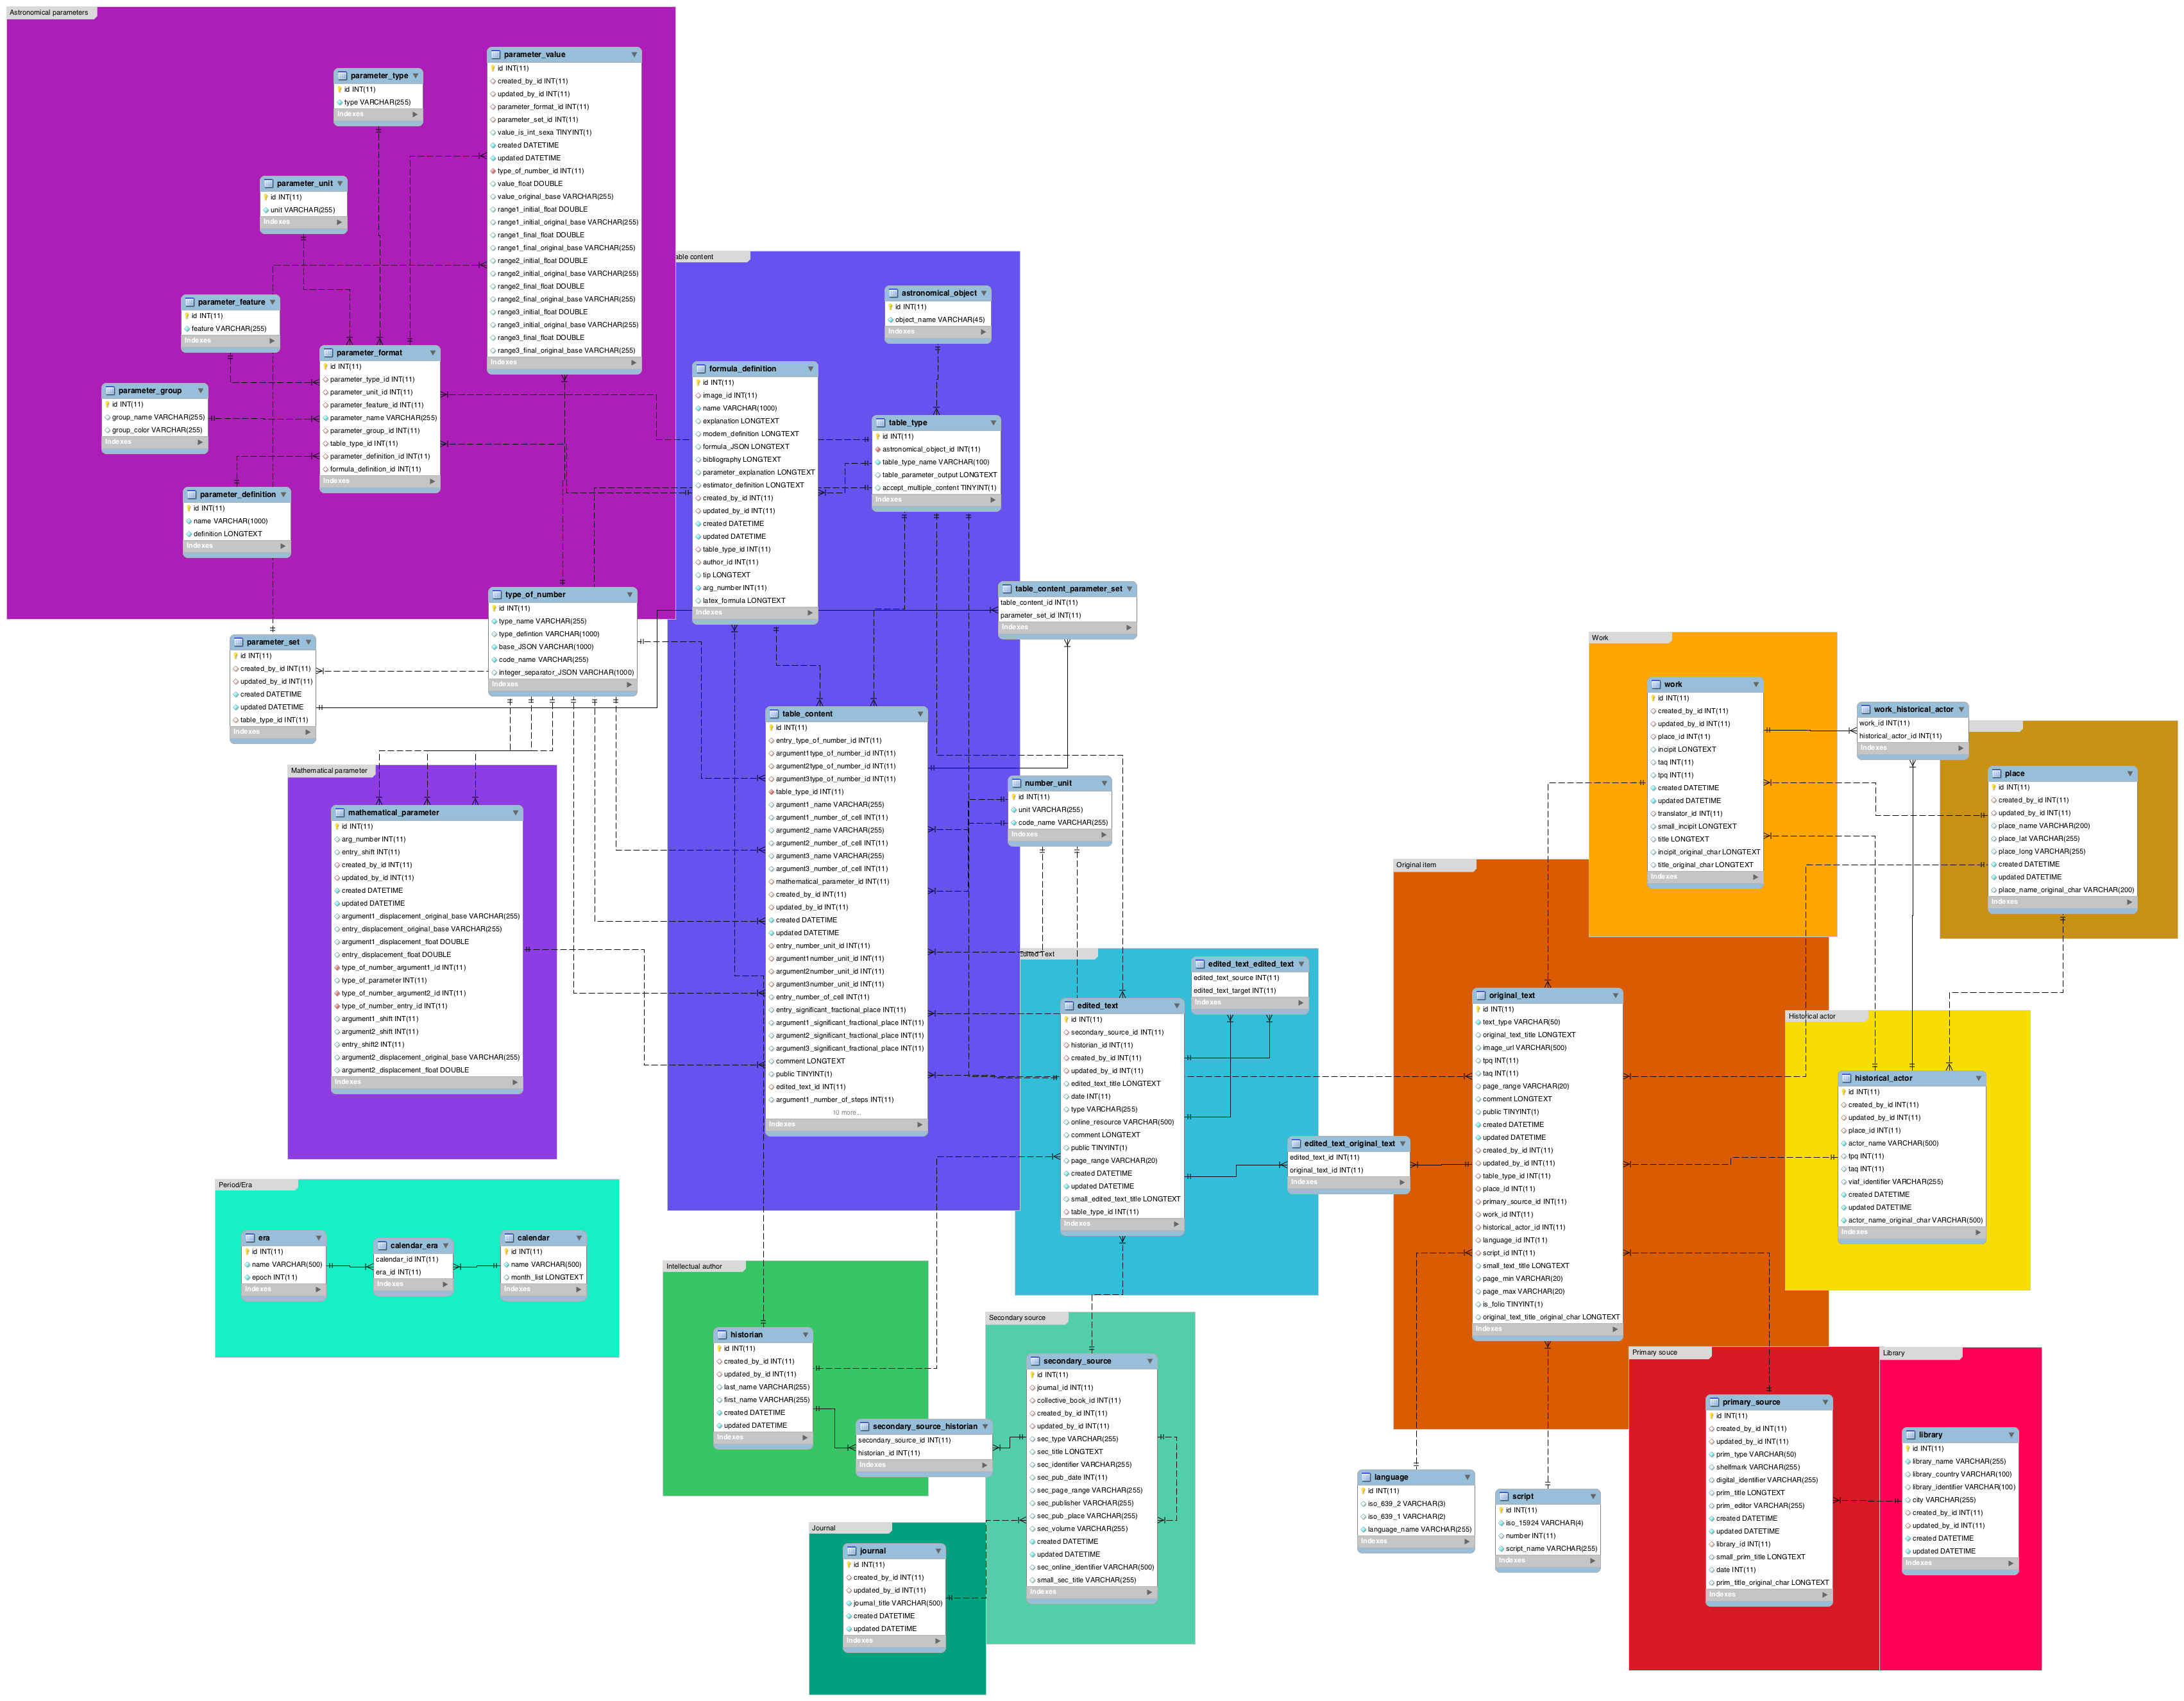
\includegraphics[width=18cm]{Annexes/Schema-Base_de_donnees.png}
		\caption{Schéma de la base de données réalisé avec \emph{MySQL Workbench}}
	\end{sidewaysfigure}
	
	Ce schéma, réalisé avec \emph{MySQL Workbench}, exclut les tables ne concernant pas la description du corpus de recherche, c'est-à-dire les tables structurelles comme celles liées à la gestion des utilisateurs.
	
\clearemptydoublepage

	\chapter{\label{Glossaire}Glossaire}
		\section{Astronomical object}
	An astronomical object is a celestial entity associated with some natural phenomena. In \textsc{dishas}, astronomical objects are used as a way to classify astronomical tables in broader categories.
	
		\section{Astronomical parameter set}
	A parameter set is a set of astronomical quantities that describes tables at the level of astronomical theories. A parameter set can be shared by several tables across different traditions. Broadly speaking, there are two kinds of parameters:
	\begin{itemize}
		\item explicit parameters that are directly read off the table, e.g., the maximum value(s);
		\item implicit parameters that need to be retrieved from the table content computationally, e.g, solar eccentricity.
	\end{itemize}
	
	In some cases, these explicit or implicit parameters are only significant in groups; whereas in other instances, parameters can be independently significant. Parameters are a central tool in delineating and connecting astronomical traditions and analysing the mathematical and astronomical content of the tables.
	A parameter-set is only linked to an intellectual author through an edited text because a single parameter-set can be shared by many different sources.
	
		\section{Edited text}
	An edited text is a production credited to a contemporary intellectual author or historian. It documents one specific table, text, or diagram. This document can be from a previous edited source or a new edition created using the web interface of \textsc{dishas}.
	
	An edited text can have various edition-types including an edition of a specific original text, a recomputation, a new production based on multiple sources, etc. An essential goal of the database is to make editions of astronomical tables that are accessible and comparable. In achieving this, edited texts, as classified in various edition-types, help identify mathematical and astronomical parameters, examine and develop critical and computational tools for creating new editions, and provide a centralised resource for studying astronomical tables from different traditions.
	
	We collect general information about the edition, e.g., the title, the date of creation, etc., to record the metadata associated with it. This, along with the other information associated with the edited text, helps us unify and create standards for comparison in our database. We collect secondary source information for bibliographic accuracy and catalogue reference.
	
		\section{Historical actor}
	Historical actors are individuals or collectives related to the items or works stored in the database. They include author, copyist, owners, dedicatee, etc. associated to the materials of the original item. Within the framework and scope of our database, we collect certain information related to the historical actors, namely, their name, their flourit, and their location, to enable us to create a standardised lists of actors.
	
	With the additional (and highly recommended) Virtual International Authority File (\textsc{viaf}) number recorded, the database makes it possible to align names added at a latter stage with a larger, normalised, authority register of person names. We collect information about the actors in order to build prosopographic data.
	
		\section{Intellectual author}
	An intellectual author is a contemporary historian who has produced an edition that is stored in the database. This historian could be different to the person entering the data into the database. For example, in certain instances, a scholar (user) may be entering the data from an edition created by another historian (from, perhaps, an unpublished collection). The intellectual author in this case is the creator-historian and not the scholar (user).
	
	Collecting information about intellectual authors validates the factual reliability of the database. This effort helps preserve the work of previous generation of historians as a way to foster and encourage further studies. The information collected about intellectual authors helps identify modern scholarship of the edition entered in the database.
	
		\section{Journal}
	In academic publishing, a scientific journal is a periodical publication intended to further the progress of science, usually by reporting new research.
	
		\section{Library}
	A library is a present-day or last-known location where the primary source is situated. The knowledge of the physical location of the library where the primary source is held is important for establishing the reliability of the database as a research resource. Facilitated with assistance tools like \textsc{isni}, entering the library information helps the database register and identify the correct library. For other libraries (not on \textsc{isni} records), a new entry helps create a record of its existence in the database for subsequent use.
	
		\section{Mathematical parameter}
	There are two kind of mathematical parameters:
	\begin{itemize}
		\item A table is said to be “displaced” when a constant value is added to its arguments or/and its entry. The value of these added constant are the first kind of mathematical parameters.
		\item A table can also be “shifted”. This happens when the ordering of the arguments and/or entry is modified according to a permutation cycle. The number of shifts in the permutation cycle is the second type of mathematical parameters.
	\end{itemize}
	The main purpose of identifying mathematical parameters is to compare displaced and/or shifted tables with those which are not displaced or shifted. We note that both kinds of tables may rely on the same set of astronomical parameters. Mathematical parameters can be shared by different sources. Additionally, shift and displacement are peculiar kinds of mathematical techniques linked to the manipulation of table sets and as such are worthy of investigation in their own right.
	
		\section{Original text}
	An original item is a table, text, or diagram as it appears in a given primary source. In instances where the actual state of the item is the result of several distinctive production acts, e.g., an extra column added to a table by a later actor, each differing state is a specific item. A scholar (user) may input these instances as separate original items. In the current stage of development of \textsc{dishas}, only tables are considered; texts and diagram will be included at a later stage.
	The original item, as it appears in the primary source, is the fundamental unit of the database. Hence, elementary units are individual tables, diagrams, or texts that are actually witnessed in specific primary sources. This level of granularity is central to make \textsc{dishas} an efficient tool for mathematical analysis and critical editing.
	
	We collect material information about the original item to allow source criticism. These include the date and the place of production, the title of the work, the manuscript shelfmark, etc.
	
		\section{Place}
	The definition of a place depends on the object to which it relates. For an original item, it refers to the place of production. For an author, it refers to his main place of activity where his work can be (approximately or accurately) geo-localised. For a work, the place refers to the original place of conception. This information is important to understand the diffusion and circulation of items in various works and traditions.
	
	Collecting information about the place, including, in some instances, its latitude and longitude, helps us represent the locations on a map. This visual representation can become an important tool for textual analysis and circulation studies.
	
		\section{Primary source}
	A primary source is a manuscript or an early printed edition in which the original item is found. It is essential for the reliability of \textsc{dishas} that it provide accurate identification of its primary sources. Additionally, having accurate information about primary sources in the database can prove to be an important tool to study the history of modern collections in astral sciences.
	
	Information about the primary source helps us identify the physical institution or library that holds the primary source. This identification allows scholars to locate the original source for further investigation.
	
		\section{Secondary source}
	A secondary source is a book, an article, a chapter, etc. that indicate a contemporary edition, or a survey of the table. Any edited document in the database can only be linked to a single secondary source for breivity. Information about secondary sources provides a reliable and tractable resource for further studies. This information will help current and future scholars use the database for their research.
	
		\section{Table content}
	The table content is the collection of numerical values in the edited text. The relation between these numerical values and those attested in the original item(s) associated with the edited text depends on the edition-type selected. We understand edited text as the type of work done by the intellectual author responsible of its creation.
	
	Comparing numerical contents of various tables and building new computational and analytic tools is central to the aim of \textsc{dishas}. In order to achieve this, a minimum level of standardisation in the layout of tables and the format of recorded numbers is necessary. However, it is equally important to allow a certain level of flexibility to reflect the practices of historical actors faithfully. Hence, there are several possibilities about table layout, table types, and types of numbers. The choices of an intellectual author are carefully documented to ensure a meaningful comparison between the table contents of various edited texts.
	We collect information about the table contents in order to structure the contents for displaying purposes. The astronomical parameters are linked to the edited texts (and not to the original text) because a given parameter set is always attributed to a table by an intellectual author after analyses.
	
		\section{Table type}
	Table are classified in different types. These different types correspond to the specific steps in astronomical computations as organised by historical actors. In modern terms, these types correspond to distinct mathematical functions which express a portion of an underlying astronomical theory.
	
		\section{Type of edition}
	Three types of edition are defined in \textsc{dishas}
	
				\subsubsection{Type-A : Edition Numerically consistent table}
	The first stage involves the rendition of the individual table (taken from individual MSS of the same work) from its diplomatic transcription onto a more numerical consistent form, i.e., a numerical format free of any data integrity errors. The following is a list; albeit not an exhaustive one, of the different types of strategies employed in creating a numerically consistent table.
	\begin{enumerate}
		\item The first stage involves the rendition of the individual table (taken from individual MSS of the same work) from its diplomatic transcription onto a more numerical consistent form, i.e., a numerical format free of any data integrity errors. The following is a list; albeit not an exhaustive one, of the different types of strategies employed in creating a numerically consistent table.
		\item Numerical parsing on a local and global scale to keep regularity, e.g., correcting a number to maintain simple mathematical regularity. It should be noted here that this inspection is merely observational and not computational.
		\item Using pattern recognition and visual inspection to correct numbers for constancy, uniformity, and accuracy (in reproduction).
		\item Noting all numerical changes, e.g., instances where ambiguous, dubious, or inconsistent numbers are altered, alternatives or originals are duly noted as comments.
	\end{enumerate}
	Note: Any ancillary material (paratext, scribal error marks and corrections, change in handwriting, etc.) is NOT included in this table: these remain features that are to be noted in the TEI version of the table.
	
				\subsubsection{Type-B : Edition Numerical Reproduced Table}
	The second stage involves employing the different individual tables (belonging to the same work, but taken from different MSS) and forming an EDITION table. This process can be defined based on a few different strategies:
	\begin{enumerate}
		\item Any eclectic, stemmatic, or copy-text method (in general, any philological method) of comparing the different 'witness' tables (from Part A) and establishing a critical 'base' numerical table, with all variants duly noted in comments. These comments effectively make the apparatus criticus.
		\item Any mathematical method (from Part C) of establishing a critical 'base' numerical table and then employing tables (from Part A) to note the variants.
		\item Any combination of the two strategies above.
		\item Additionally, any previously 'critically' edited table (from a set of extant or non-existing manuscripts) belonging to the same table-type and work (as set in Part A) can also be stored in Part B here. In such cases, it is important to note any relation, if applicable, of this previous work to the different tables in Part A. Failing this, a common reference to the work and table- type becomes minimally necessary.
	\end{enumerate}
	Several different 'critical editions' (based on different editorial strategies) of the same table may be stored in this stage; all of which, are identified with the correct relational structure to the tables in parts A and C.
	
				\subsubsection{Type-C : Edition Numerically Recomputed Table(s)}
	The third stage involves the recomputed tables –~corresponding to each individual table in Part A~– that are stored relationally in the SQL database. These tables are generated based on the following possible strategies:
	\begin{enumerate}
		\item A modern mathematical recomputation of the table based on (a) choice of appropriate parameter, (b) mathematical equations governing the underlying function tabulated, (c) selection of a suitable generative or iterative algorithm.
		\item A historically congruous mathematical algorithm based on editorial decisions. These tables are generated by a modern scholar based on his or her own understanding of the mathematical apparatus presumably intended to have been used by the original author in his time. These tables form a collection of our modern efforts to reconstruct numerical tables within its historical context.
		\item Any other derivatives or combinations of mathematical procedures, algorithms, iterative techniques, rounding schemes, etc. used to generate the numerical entries of the table form separate mathematical tables that are also stored in this part.
	\end{enumerate}
	
		\section{Work}
	An astronomical work is a distinct intellectual creation consisting of tables, texts, or diagrams. It is often identified by a title or incipit and attributed to a given historical actor. Its content and organisation may vary depending on the particular primary source.
	
	We can analyse the different attestations of a given work as original items rather than individual works are the fundamental unit of \textsc{dishas}. For instance, one can identify a core set of tables around which various satellites tables, texts, or diagrams may be presented depending on the primary source. With this design, the geographical and chronological evolution of these dynamical sets of original items can be analysed and studied. This ability is essential when it comes to critical editing a work. Additionally, the choice of an original item as the fundamental unit also allows to analyse the intellectual composition of a given manuscript. This is an important step in understanding how manuscript shape intellectual traditions.
	
	A work needs to be identified by a current title or incipit. When possible supplementary information like place, dates, authors or translator is very useful for studying the circulation of the work.
	
\clearemptydoublepage

	\chapter{\label{BackOffice}Captures d'écrans de l'interface administrateur}
	\begin{figure}[h!]
		\centering
		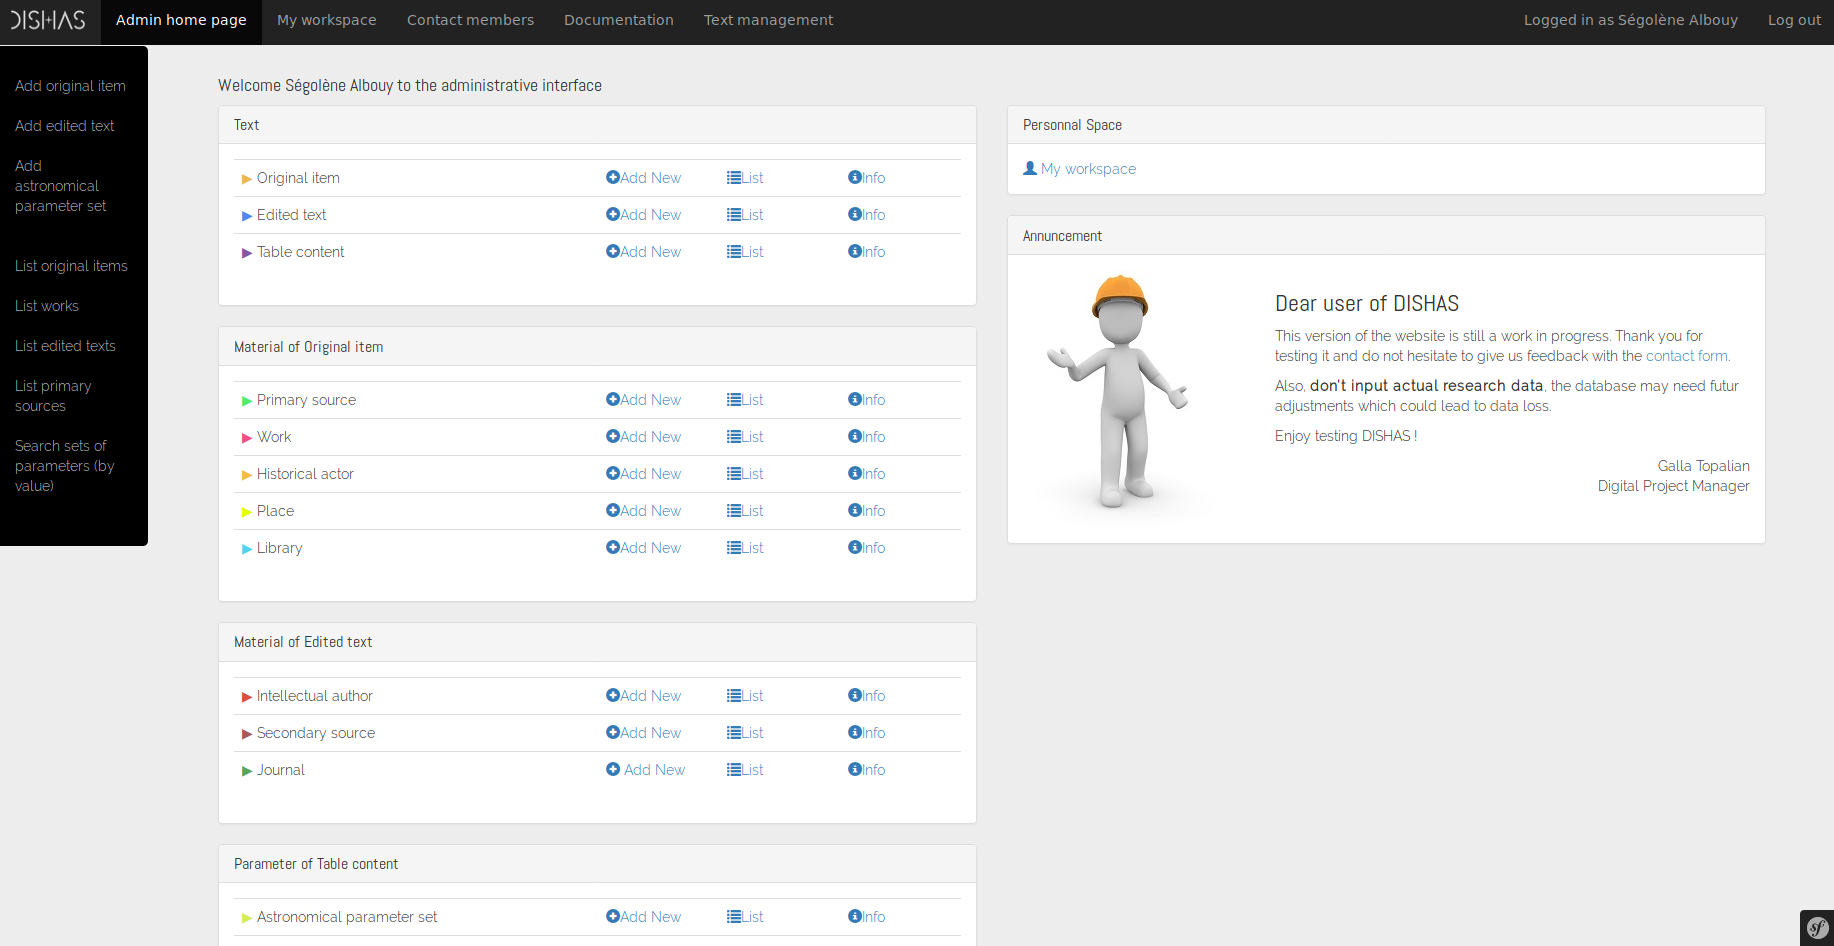
\includegraphics[width=17cm]{Annexes/Captures_ecrans/Interface_administrateur/Homepage.png}
		\caption{Page d'accueil de l'interface administrateur}
	\end{figure}

	\begin{figure}[h!]
		\centering
		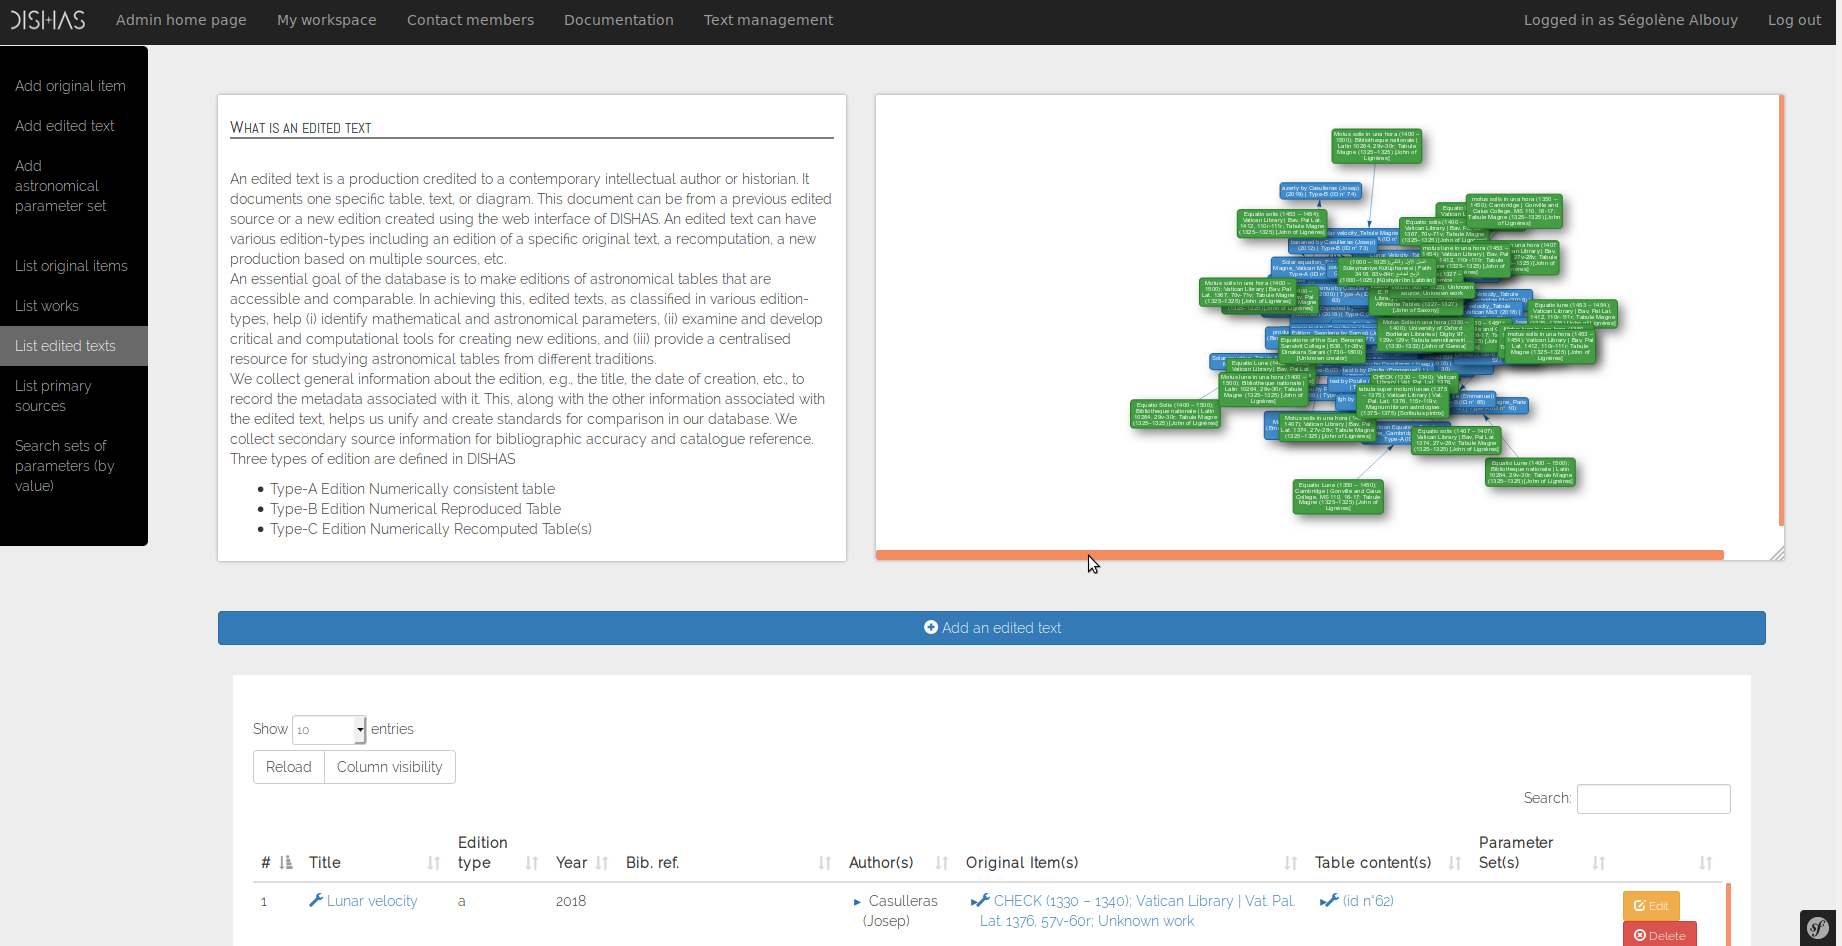
\includegraphics[width=17cm]{Annexes/Captures_ecrans/Interface_administrateur/List-Edited_texts.png}
		\caption{Page de liste des enregistrements des éditions de tables astronomiques}
	\end{figure}

	\begin{figure}[h!]
		\centering
		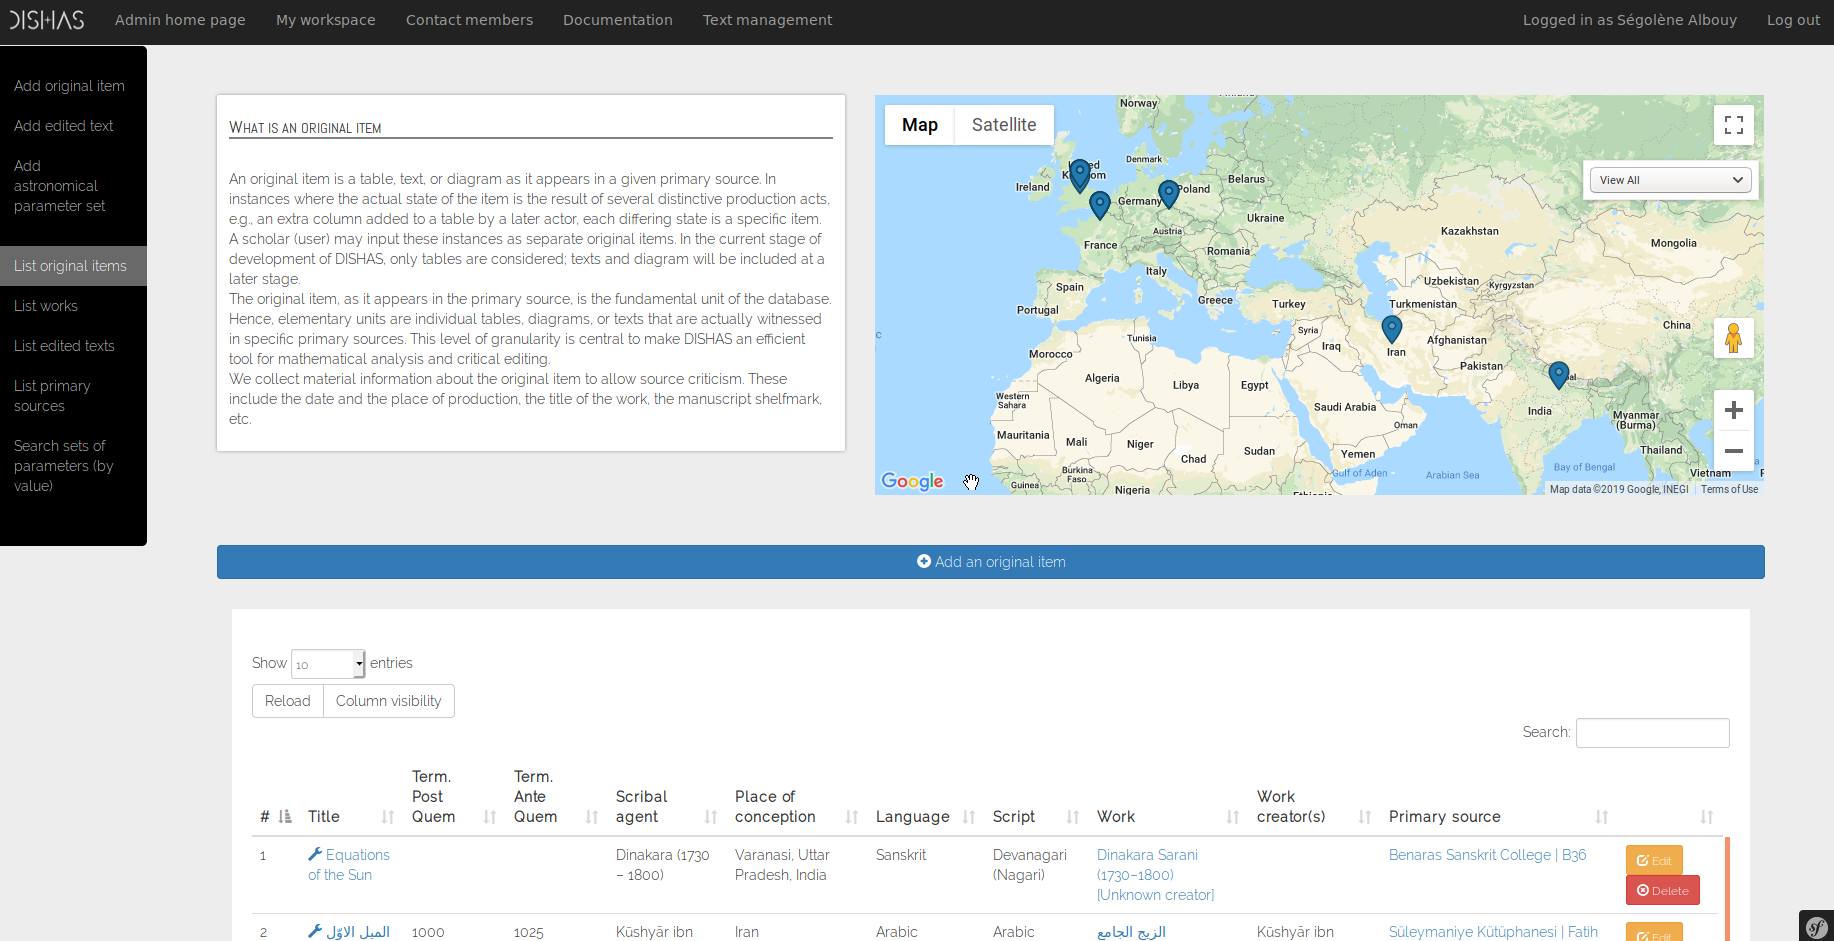
\includegraphics[width=17cm]{Annexes/Captures_ecrans/Interface_administrateur/List-Original_items.png}
		\caption{Page de liste des enregistrements des \ois}
	\end{figure}

	\begin{figure}[h!]
		\centering
		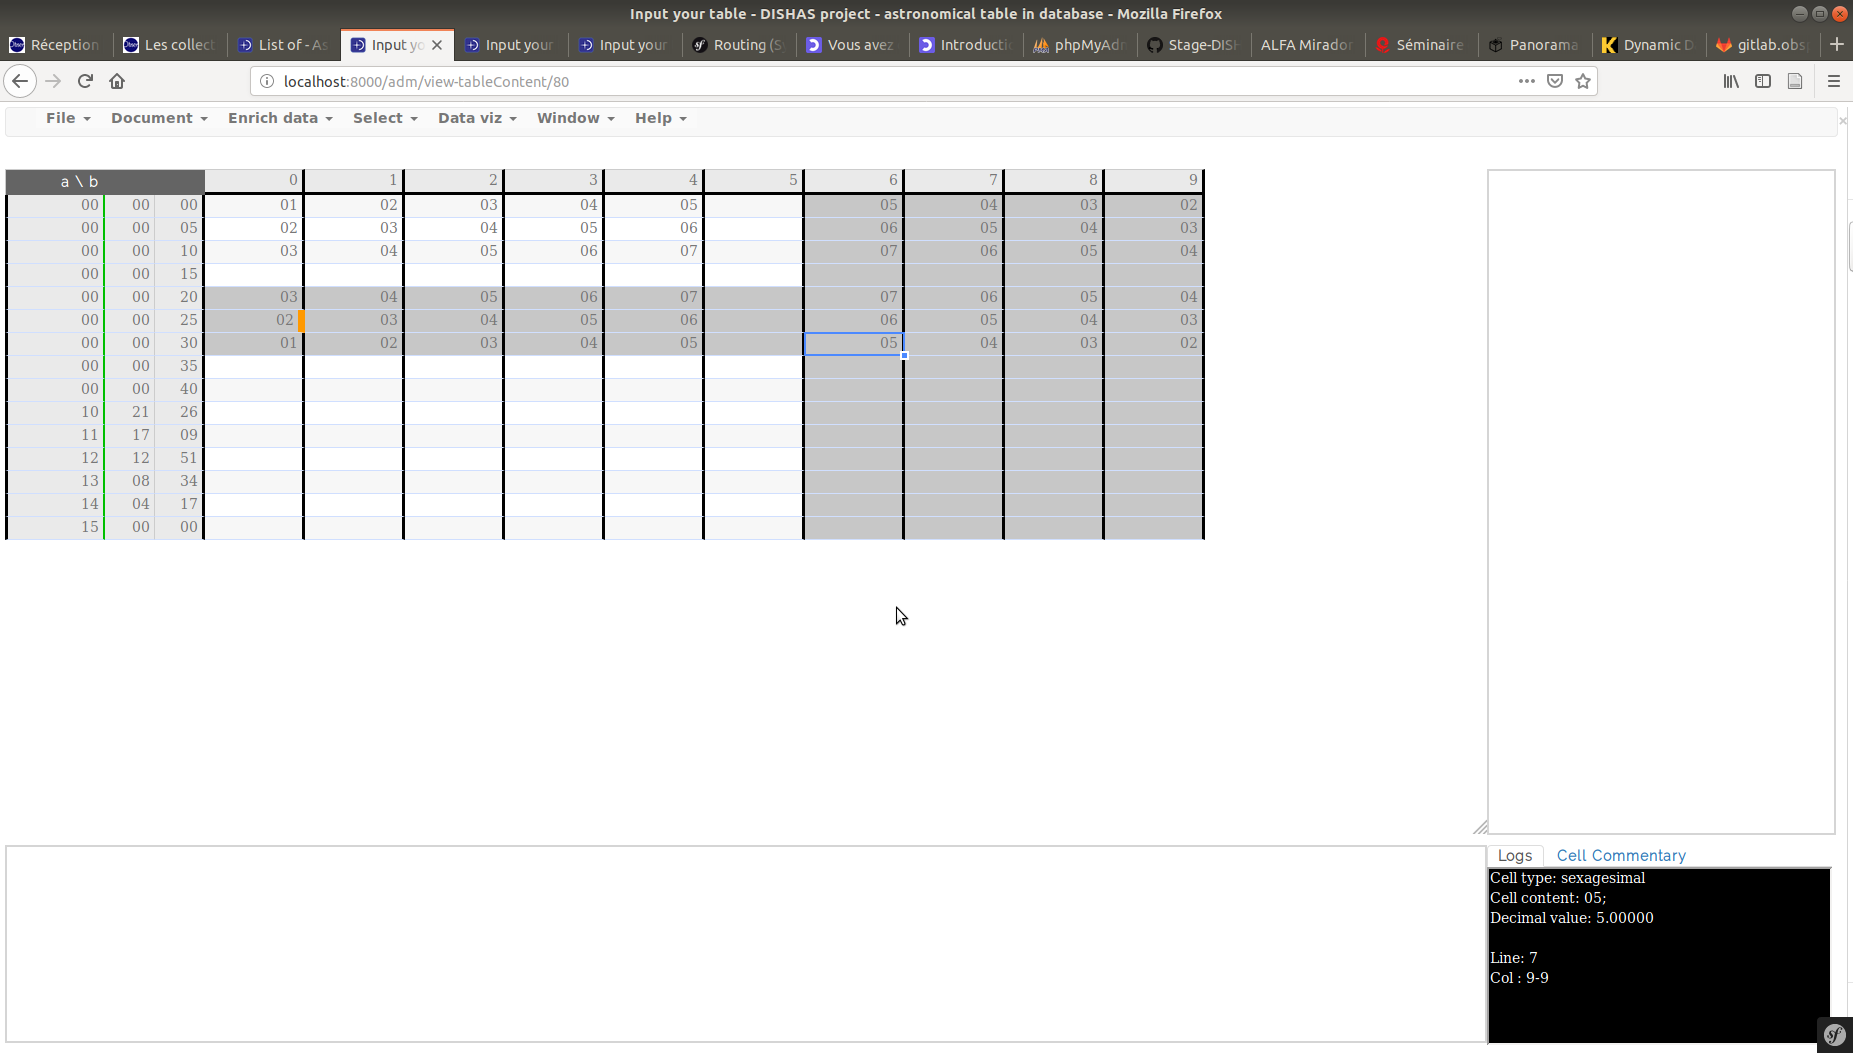
\includegraphics[width=17cm]{Annexes/Captures_ecrans/Interface_administrateur/DISHAS_Table_Interface.png}
		\caption{Interface de saisie numérique de tables}
	\end{figure}

\clearemptydoublepage

	\chapter{\label{PresentationSeminaire}Présentation du \eng{front office}}
	Document de présentation utilisé lors du séminaire numérique de l'équipe de DISHAS du 13 mai 2019, en présence de l'équipe de recherche. Certaines diapositives ont été retirées du document pour éviter la redondance de l'information. Cette présentation visait à exposer les propositions de développements concernant les parties de l'interface utilisateur.
	
	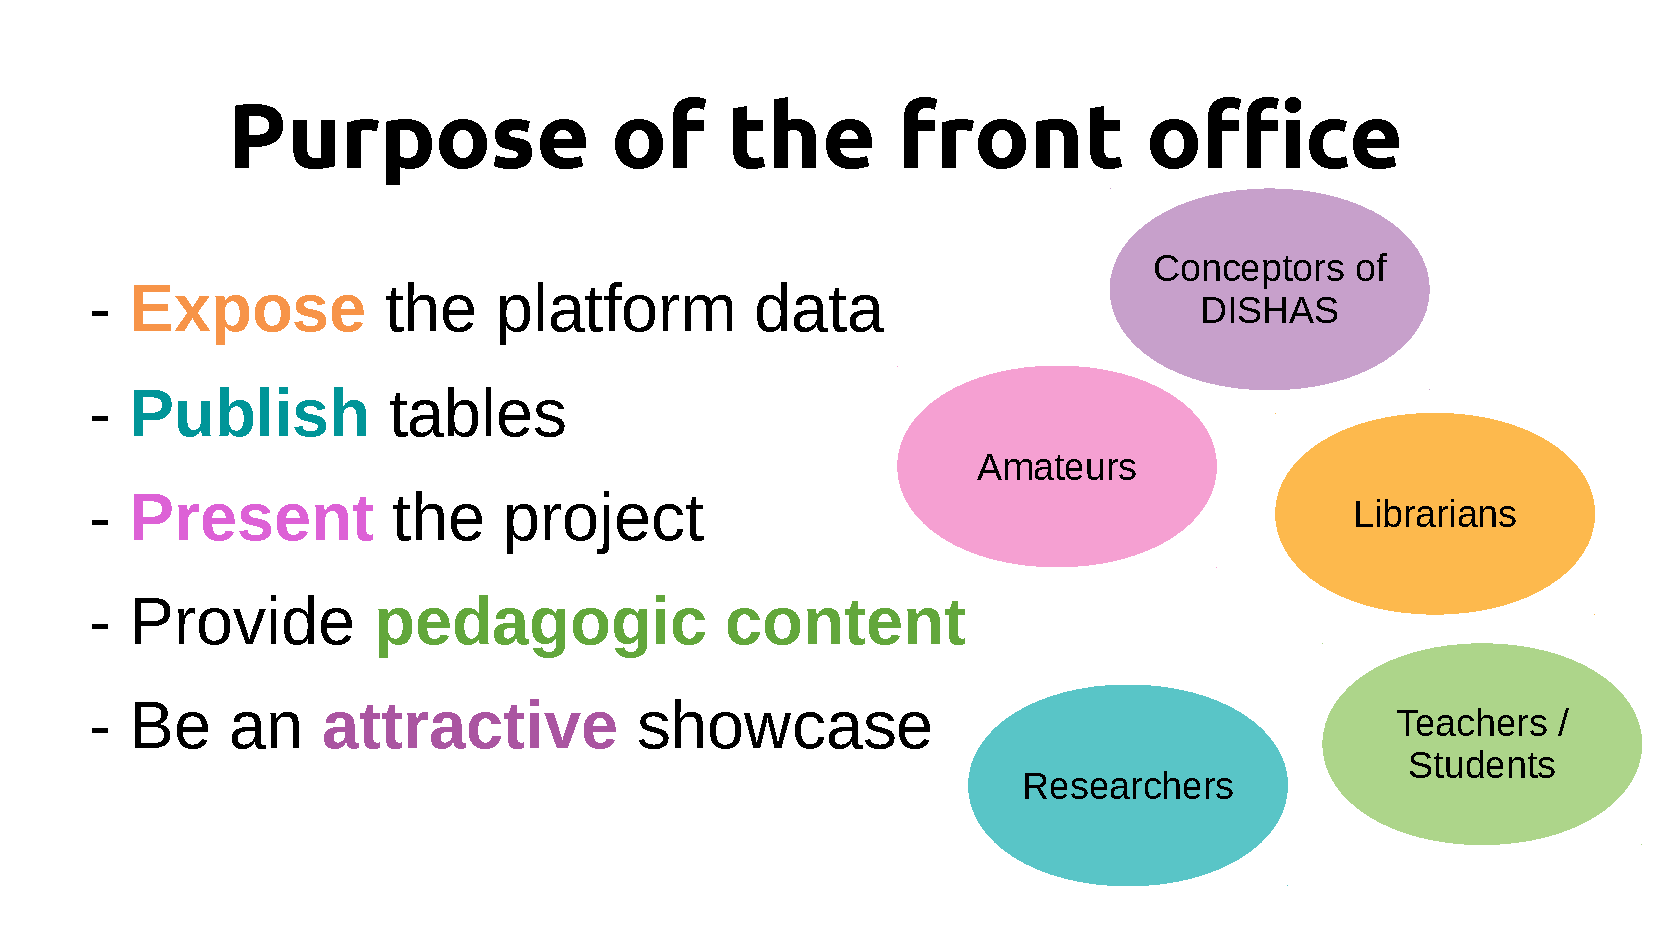
\includepdf[nup=1x2,pages=-, scale=0.9]{Annexes/2019-05-13-Presentation-seminaire.pdf}

\clearemptydoublepage

	\chapter{\label{CahierDesCharges}Cahier des charges fonctionnel des visualisations pour l'interface utilisateur}
	Ce document est un cahier des charges fonctionnel où sont décrites en détail toutes les interfaces de la plateforme publique~; chaque rangée correspond à une page de la plateforme, chaque colonne concernant quant à elle un aspect précis de cette page~:

	\begin{itemize}
		\item une première colonne présente l'interface de manière générale~: son objectif, son architecture globale avec la description de ses différents composants ainsi qu'éventuellement des interrogations vis-à-vis de sa conception~;
		\item une deuxième colonne expose l'ensemble des données qui seront récupérées de la base pour l'affichage, en particulier pour les métadonnées requises dans les pages de notices~;
		\item une troisième colonne s'attache à expliciter précisément la visualisation de donnée apparaissant sur la page (si tel est le cas), tant dans son aspect visuel que dans ses enjeux intellectuels~;
		\item une quatrième colonne concerne les données nécessaires à la constitution de cette visualisation~;
		\item une cinquième colonne dresse la liste de tous les liens de redirection présents à l'intérieur de la page, composant ainsi le réseau dans lequel elle s'inscrit~;
		\item une dernière colonne détaille les corpus de données qui pourront être établit à partir de cette page. Cette partie concerne essentiellement les pages de notice, et fait référence aux \g{loupes} disposées sur la barre latérale de métadonnées.
	\end{itemize}

	\begin{landscape}
		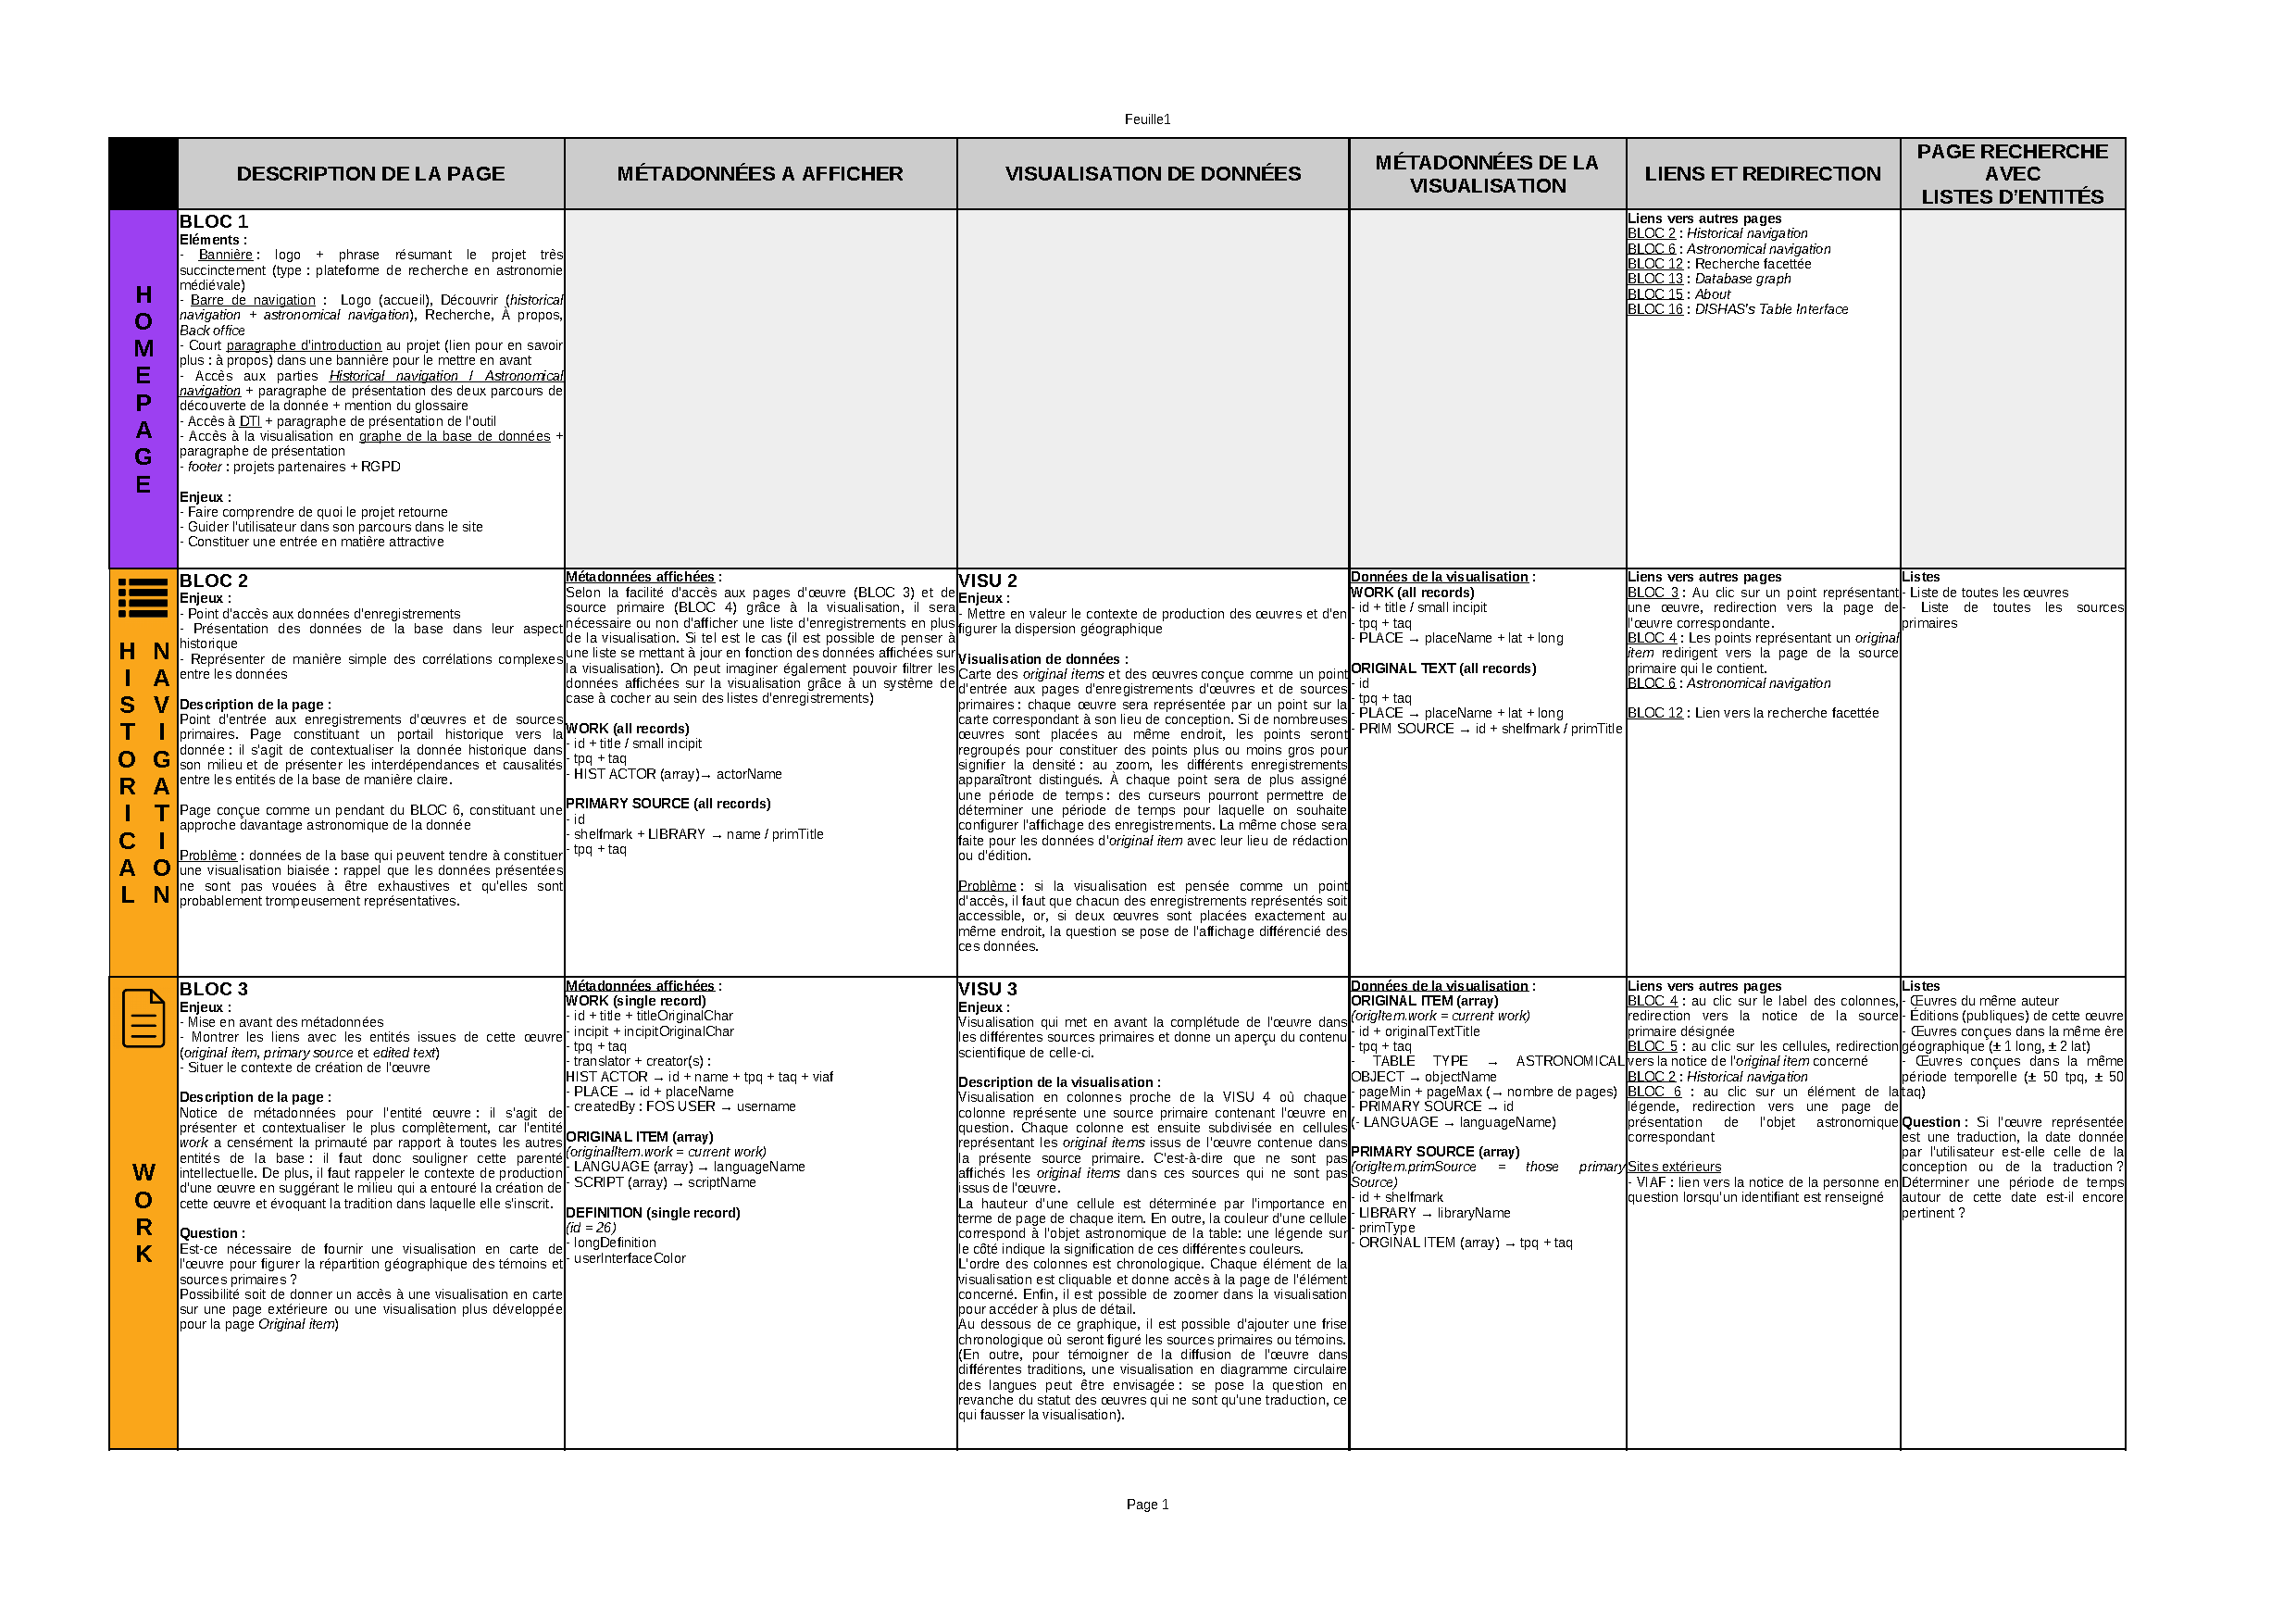
\includepdf[pages=-, scale=1,landscape=true]{Annexes/Cahier-des-charges-visualisations.pdf}
	\end{landscape}
	
\clearemptydoublepage

	\chapter{\label{ElasticSearch}Exemples de requêtes avec ElasticSearch}
		\section{ElasticSearch query language}\label{elasticsearch-query-language}
	
	ElasticSearch has its own query language, more documentation can be
	found \href{https://www.elastic.co/guide/en/elasticsearch/reference/current/query-dsl.html}{here}
	
			\subsection{Anatomy of a query}\label{anatomy-of-a-query}
	
	In most cases, an ElasticSearch query is composed of :
	\begin{itemize}
		\item a \textbf{header} defining~:
		\begin{itemize}
			\item which \textbf{\emph{method}} is to be used~: \texttt{GET}, \texttt{POST}, etc.
			\item which \textbf{\emph{index}} (i.e.~which entity of the database written in snake\_case) is going to be queried. Not necessary if all indexes will be queried.
			\item what \textbf{\emph{type}} of search is to be made (\texttt{\_search} most of the time)
		\end{itemize}
		\item a \textbf{body} defining (among other things)~:
		\begin{itemize}
			\item the \textbf{\emph{fields}} that are going to appear in the results (\texttt{\_source})
			\item the \textbf{\emph{filters}} that are going to narrow the number of results matching those filters (\texttt{query})
			\item different properties of the results (size of the results, index from which to begin, etc.)
		\end{itemize}
	\end{itemize}

				\paragraph{Tips \& tricks}\label{tips-tricks}

The body of a query needs to be a correctly formatted JSON string, even using single quotes instead of double is considered to be an error. The \texttt{dev tools} tab in Kibana interface offers help for automatic indentation and autocompletion features that can be very handy.

		\subsection{Get all records}\label{get-all-records}

To get all the records of the entire database :

\begin{lstlisting}
GET _search
\end{lstlisting}

To retrieve all records from an index (primary source in this case) :

\begin{lstlisting}
GET primary_source/_search
\end{lstlisting}

Which is equivalent to :

\begin{lstlisting}
GET primary_source/_search
{
    "query": {
        "match_all": {}
    }
}
\end{lstlisting}

		\subsection{Simple \href{https://www.elastic.co/guide/en/elasticsearch/reference/current/query-dsl-match-query.html}{matching query}}\label{simple-matching-query}

				\paragraph{Exact term match}\label{exact-term-match}

\begin{quote}
	All the works that contain the string ``tabule'' in their title.
\end{quote}

Note that the case of the letters doesn't matter, it will match ``Tabule'' as well. In addition to that, in this configuration, a sub-string will not match the same as the entire string (``tabu'' will not match ``tabule'') ; the string is treated as a complete word.

\begin{lstlisting}
GET work/_search
{
    "query":{
        "match": {
            "title": "tabule"
        }
    }
}
\end{lstlisting}

\begin{quote}
	All the original items that are associated with a primary source that is kept in the library that have \texttt{2} as id.
\end{quote}

\begin{lstlisting}
GET original_text/_search
{
    "query": {
        "match": {
            "primary_source.library.id": "2"
        }
    }
}
\end{lstlisting}

				\paragraph{Multiple terms match}\label{multiple-terms-match}

\begin{quote}
	All original items that have in their title either the word ``solis'', either the word ``lune''.
\end{quote}

In this configuration, each string separated by a space is treated individually and the operator used to connect them is \texttt{OR}. In other words, the more you put terms, the more you will match original items.

\begin{lstlisting}
GET original_text/_search
{
    "query": {
        "match": {
            "original_text_title": "solis lune"
        }
    }
}
\end{lstlisting}

To get a response where each terms given are independently going to filter the result (same kind of behavior as a Google query), you need to specifies the operator to be \texttt{AND}.

\begin{lstlisting}
GET original_text/_search
{
    "query": {
        "match": {
            "original_text_title": {
                "query": "lune solis",
                "operator": "AND"
            }
        }
    }
}
\end{lstlisting}

		\subsection{Adding some margin of error}\label{adding-some-margin-of-error}

				\paragraph{Fuzziness}\label{fuzziness}

The fuzziness allows a certain amount of inaccuracy to be accepted.

\begin{quote}
	All library that approximately have the string ``natonale'' in their name.
\end{quote}

\begin{lstlisting}
{
    "query": {
        "match": {
            "library_name": {
                "query": "natonale",
                "fuzziness": "auto"
            }
        }
    }
}
\end{lstlisting}

You can set the fuzziness to \texttt{1} or more but the \texttt{auto} settings allows a number of letters that do not match, proportional to the length of the term to be searched.

			\subsubsection{Full text search on an index}\label{full-text-search-on-an-index}

To allow search on every field of an entity, the query has to be set to \texttt{multi\_match}.

\begin{quote}
	All edited texts that have approximately the string ``lune'' in one of them fields.
\end{quote}

\begin{lstlisting}
GET edited_text/_search
{
    "query": {
        "multi_match": {
            "query": "lune",
            "fuzziness": "auto"
        }
    }
}
\end{lstlisting}

As is, those kind of requests are deprecated because no fields are specified : ElasticSearch encourages to list the fields you want the query to be executed on. The \texttt{fields} allows to reduce noise in the results and to take less time.

\begin{quote}
	All primary sources that match approximately the strings ``vatican'' and ``latin'' in the list of fields specified.
\end{quote}

\begin{lstlisting}
GET primary_source/_search
{
    "query": {
        "multi_match": {
            "query": "vatican latin",
            "fuzziness": "auto",
            "operator": "and",
            "fields": [
                "shelfmark",
                "digital_identifier",
                "kibana_name",
                "tpq.keywork",
                "taq.keywork",
                "prim_type",
                "library.kibana_name",
                "original_texts.kibana_name",
                "original_texts.table_type.kibana_name",
                "original_texts.place.kibana_name",
                "original_texts.historical_actor.kibana_name",
                "original_texts.script.script_name",
                "original_texts.language.language_name"
            ]
        }
    }
}
\end{lstlisting}

Notice that on the fields \texttt{tpq} and \texttt{taq} that are typed as integer, a string query cannot be performed. In order to query those fields as well, you must add \texttt{.keyword} after the field name : it corresponds to the field but typed as a string.

				\paragraph{Wildcards}\label{wildcards}

To find some more documentation for wildcard queries, click \href{https://www.elastic.co/guide/en/elasticsearch/reference/current/query-dsl-wildcard-query.html}{here}.

		\subsection{Defining the source}\label{defining-the-source}

If you are not interested in all the metadata (i.e.~the content of the fields) associated with the entity you want to query, it is possible to set a list of fields that are going to appear in the response.

\begin{quote}
	Only the shelfmark, and the library name of all primary sources that are a manuscript
\end{quote}

\begin{lstlisting}
GET primary_source/_search
{
    "_source": [
        "shelfmark",
        "library.library_name"
    ],
    "query": {
        "match": {
            "prim_type": "ms"
        }
    }
}
\end{lstlisting}

Note that if a record in the result do not have some information you asked for (let's say, the primary source isn't associated with a library, thus doesn't have a \texttt{library.libray\_name}), the result object will not have the key for this precise field. Instead of looking like that :

\begin{lstlisting}
"_source" : {
    "library" : {
        "library_name" : "Vatican Library"
    },
    "shelfmark" : "Vat. Pal. Lat. 1376"
}
\end{lstlisting}

It will look like :

\begin{lstlisting}
"_source" : {
    "shelfmark" : "Vat. Pal. Lat. 1376"
}
\end{lstlisting}

		\subsection{Special queries}\label{special-queries}

			\subsubsection{\href{https://www.elastic.co/guide/en/elasticsearch/reference/current/query-dsl-range-query.html}{Range queries}}\label{range-queries}

Range queries can be made on fields that are numbers (even if the field is typed as a string but contains integer) in the Kibana interface, but does seem to only work on integer/float/date typed field when using ajax.

\begin{quote}
	All the primary source that have an edition date between 1400 and 1500
\end{quote}

\begin{lstlisting}
GET primary_source/_search
{
    "query": {
        "range": {
            "date": {
                "gte": 1400, // greater than
                "lte": 1500 // less than
            }
        }
    }
}
\end{lstlisting}

If you want to make a range query on a date typed field (fields that end with \texttt{\_date}, you can use some ElasticSearch \href{https://www.elastic.co/guide/en/elasticsearch/reference/current/common-options.html\#date-math}{tools for date math} (those as well, seems to cause problem when used with ajax) :

\begin{quote}
	All original items that have been created between 1000 years before today and 25 years after 1500
\end{quote}

\begin{lstlisting}
GET original_text/_search
{
    "query": {
        "bool": {
            "must": [
                {
                    "range": {
                        "tpq_date": {
                            "gte":"now-1000y"
                        }
                    }
                },
                {
                    "range": {
                        "taq_date": {
                            "lte": "1500-01-01||+25y"
                        }
                    }
                }
            ]
        }
    }
}
\end{lstlisting}

			\subsubsection{\href{https://www.elastic.co/guide/en/elasticsearch/reference/current/query-dsl-geo-distance-query.html}{Geo-distance} queries}\label{geo-distance-queries}

The fields named \texttt{location} holds information that is treated as geo point by ElasticSearch : \texttt{geo\_distance} queries can be executed on them.

\begin{quote}
	All works that have been conceived around 100km from 48 of latitude and 2 of longitude. \textbf{NB} : in this syntax, \texttt{longitude} comes before \texttt{latitude}.
\end{quote}

\begin{lstlisting}
GET work/_search
{
    "query": {
        "geo_distance": {
            "distance": "100km",
            "place.location": [2,48]
        }
    }
}
\end{lstlisting}

The same query can be formulated more explicitly with this syntax :

\begin{lstlisting}
GET work/_search
{
    "query": {
        "geo_distance": {
            "distance": "100km",
            "place.location": {
                "lat" : 48,
                "lon" : 2
            }
        }
    }
}
\end{lstlisting}

		\subsection{Combining multiple clauses}\label{combining-multiple-clauses}

Every filter you want to combine to build a query can be add with this kind of structure :

\begin{lstlisting}
{
    "query": {
        "bool": {
            "must": [
                {
                    // filter one
                },
                {
                    // filter two
                }
            ]
        }
    }
}
\end{lstlisting}

				\paragraph{Putting all together}\label{putting-all-together}

\begin{quote}
	The shelfmarks of all early printed primary sources that contains an original item that were created near Paris (lat : 48, long : 2).
\end{quote}

\begin{lstlisting}
GET original_text/_search
{
    "_source": [
        "primary_source.shelfmark"
    ],
    "query": {
        "bool": {
            "must": [
                {
                    "geo_distance": {
                        "distance": "100km",
                        "place.location": [2,48]
                    }
                },
                {
                    "match": {
                        "primary_source.prim_type": "ep"
                    }
                }
            ]
        }
    }
}
\end{lstlisting}

\clearemptydoublepage

\chapter{\label{Branche}Description des développements réalisés pendant le stage}

The ``Segolene-front-office'' branch mostly concerns the historical part of the navigation in the front office. Several modules where developped~:
\begin{itemize}
	\item Data visualisations~;
	\item Sidebar for metadata~;
	\item Search interface~;
	\item Bread crumbs~;
	\item Related table editions.
\end{itemize}

NB : the presented functions are here often simplified for demonstration purposes comparing to the way they are integrated into the code.

		\section{Data visualisation}\label{data-visualisation}

			\subsection{Visualisation description}\label{visualisation-description}

Three different visualisations were developped for the historical navigation with the AmCharts library :
\begin{itemize}
	\item \textbf{Column chart} : visualisation for the work record page. Each column represents a primary source divided in original items (the cells) which colors are determined by their astronomical object~; the visualisation allows to show completeness and content of the sources derived from a intellectual work.
\end{itemize}

\begin{figure}[H]
	\centering
	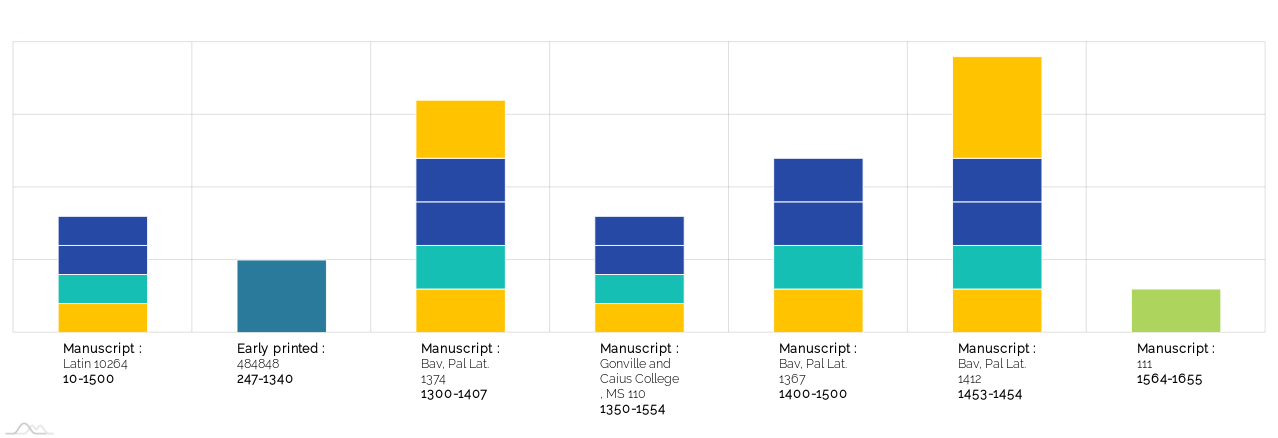
\includegraphics[width=16cm]{Images/Visualisations/Work-Tabule_Magne.png}
	\caption{Column chart for work visualisation}
\end{figure}

\begin{itemize}
	\item \textbf\textbf{Bar chart} : visualisation for the primary source record page. Each bar represents a work that is contained in the primary source, each bar being divided in original items originated from the work. A select allows two switch between two states of the visualisation : one where all pages of the items are added together, one where they are disposed accordingly to their position in the source. The visualisation thus can show the composite aspect of some primary sources.
\end{itemize}

\begin{figure}[H]
	\centering
	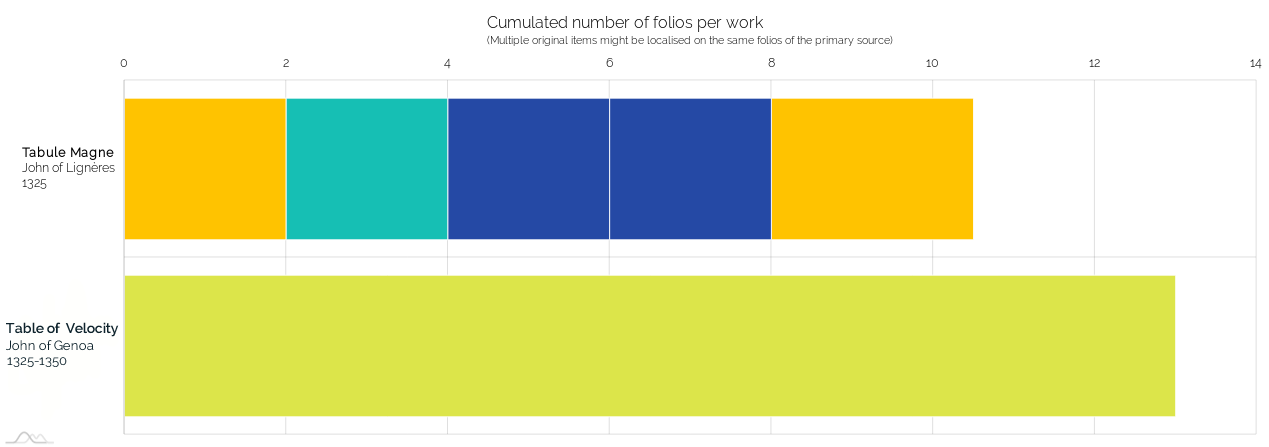
\includegraphics[width=16cm]{Images/Visualisations/Primary_source-Stacked.png}
	\caption{Bar chart for primary source visualisation~: original items stacked}
\end{figure}
\begin{figure}[H]
	\centering
	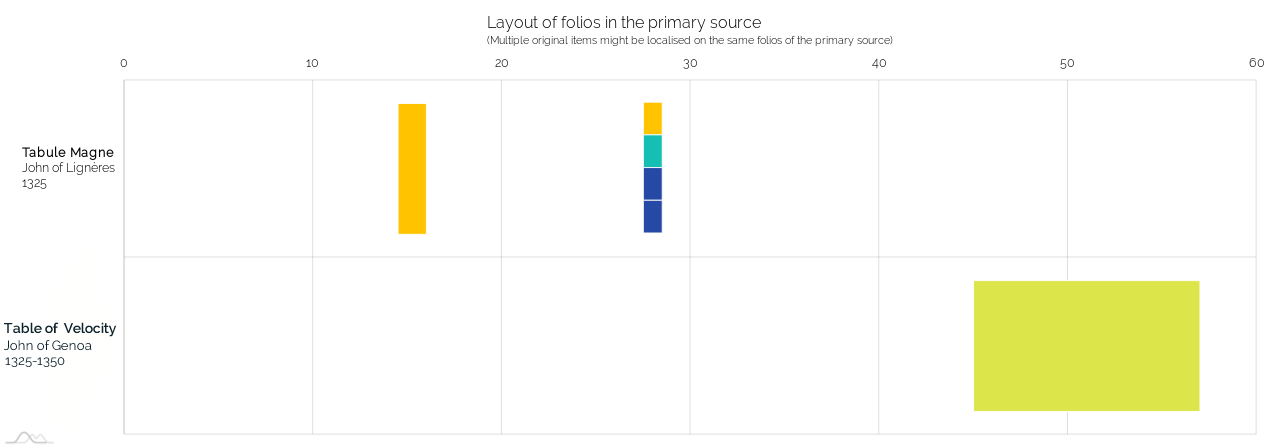
\includegraphics[width=16cm]{Images/Visualisations/Primary_source-Spread_out.png}
	\caption{Bar chart for primary source visualisation~: original items spread out}
\end{figure}

\begin{itemize}
	\item \textbf{Historical map} : visualisation for the original item records, the historical navigation and more to come. The map displays points that represent the place of creation of works (in yellow), primary sources/original items (in red) and combination of both (in orange). A heatmap underneath represents the time axis and show what period were more prolific : the scrollbar allows the user to select a time period so that only the items created during the timerange are shown.
\end{itemize}

\begin{figure}[H]
	\centering
	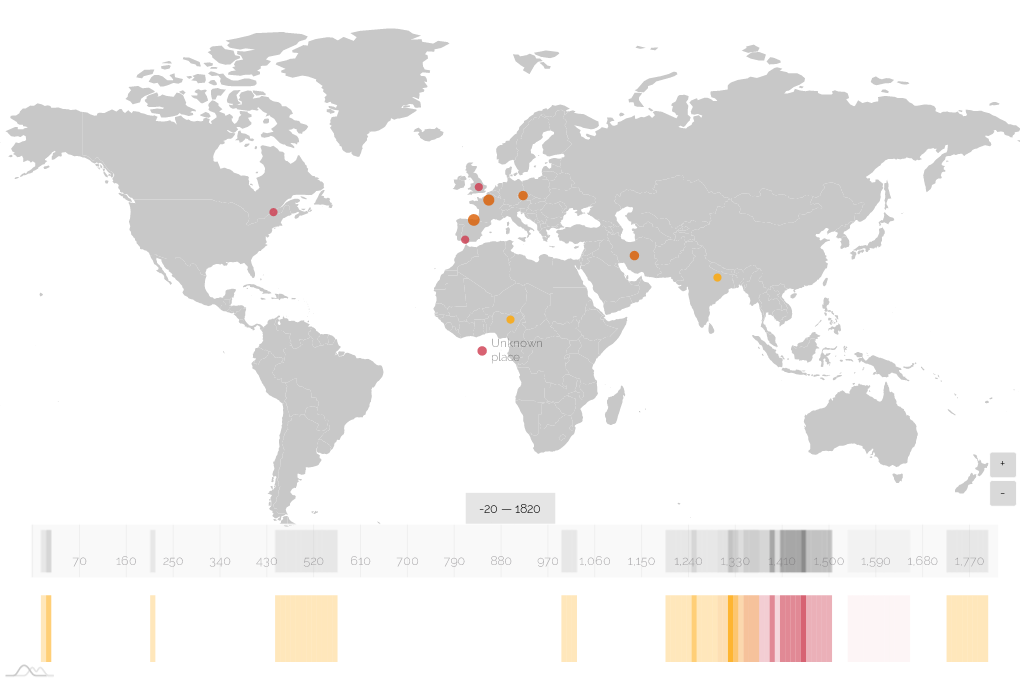
\includegraphics[width=16cm]{Images/Visualisations/Historical_navigation-All.png}
	\caption{Map for historical navigation}
\end{figure}

			\subsection{Function explanation}\label{function-explanation}

				\subsubsection{Historical map}\label{historical-map}

This function is triggered when the user change the range selected by the scrollbar. What it does is that each time the start and the end grips of the scrollbar are both outside (by being under or above it) of the \texttt{tpq} and \texttt{tap} dates of an item, the item is not shown on the map. When the grips are not both outside, the size, color, tooltip of the map point are set accordingly to the items that were created in the timerange selected.

\begin{lstlisting}
scrollbarX.events.on("rangechanged", function () {
    let cursorMin = scrollbarX.range.start;
    let cursorMax = scrollbarX.range.end;

    // Conversion of the min and max range value into date
    let dateMinRange = parseInt((cursorMin / yearRange) + startBar);
    let dateMaxRange = parseInt((cursorMax / yearRange) + startBar);
    // Show the timerange selected
    scrollbarX.startGrip.tooltipText = `${dateMinRange}`;
    scrollbarX.endGrip.tooltipText = `${dateMaxRange}`;
    timeframeLabel.text = `${dateMinRange} — ${dateMaxRange}`;

    i = 0;
    // for each place in mapData
    for (let index in mapData) {
        // defining appearance of the circle localised on the place
        let place = mapData[index];
        let opacity = 0; // if no item is to be displayed, opacity to 0
        let countW = 0; // count of the number of works to be displayed : color and radius of the circle
        let countPS = 0; // count of the number of primary sources to be displayed : color and radius
        let number = 0;

        for (let j = place.items.length - 1; j >= 0; j--) {
            let dateMin = (place.items[j].from - startBar) * yearRange;
            let dateMax = (place.items[j].to - startBar) * yearRange;
            if (!((cursorMin > dateMax && cursorMax > dateMax) || (cursorMin < dateMin && cursorMax < dateMin)))
                // when the two cursors are not both outside of the time frame selected
                // either by being under or above it
            {
                number++;
                opacity = 0.8; // set the opacity in order to not be transparent
                if (place.items[j].entity === "work") {
                    countW += 1; // add one to the count of works
                } else {
                    countPS += 1;
                }
            }
        }

        let Wtootltip = countW !== 0 ? "[bold]Work[/]\n‣ " + countW + " record(s)" : "";
        let PStootltip = countPS !== 0 ? "[bold]Primary source[/]\n‣ " + countPS + " record(s)" : "";

        let tooltip = "[font-size:18px]" + place.place + "[/]\n" + Wtootltip + PStootltip;
        number = number !== 0 ? number * 100 : 100;

        placeMarker[i].fillOpacity = opacity;
        placeMarker[i].radius = Math.log(number);
        placeMarker[i].tooltipText = tooltip;
        i++;
    }
});
\end{lstlisting}

				\subsubsection{Bar chart}\label{bar-chart}

This function is triggered when the user selects one or another option. If the option is ``page disposition'', the height and displacement of the cell are determined in relation to the number of items in the same bound as theirs. In other words, the more items there are on the same pages, the thiner and the more deported from the center will be the cell representing one item.
 
\begin{lstlisting}
function selectView(select) {
    if (select === "spread") {
        chart.data = spreadOutSet; // make the chart use the "spread out" data set
        let numberOfWorks = Object.keys(worksBounds).length;
        let heightWork = 292/numberOfWorks; // height of the horizontal part dedicated to one work
        let heightBar = 225/numberOfWorks; // height of the bar in itself

        for (let work of Object.keys(worksBounds)){
            bounds = worksBounds[work];
            for (key of Object.keys(bounds)){
                i = 0;
                let bound = bounds[key];
                let numberOfOrigItems = bound.origItems.length;
                for (let id of bound.origItems) {
                    let heightItem = heightWork/numberOfOrigItems;
                    // setting the height of the cell
                    series[id].columns.template.height = heightItem;
                    // configuring the displacement of the cell comparing to the center
                    if (heightItem !== heightWork){
                        series[id].columns.template.dy = -(heightBar/2) + (heightItem * i);
                    }
                    i++;
                }
            }
        }
    } else if (select === "stack") {
        chart.data = stackedSet; // make the chart use the "stacked" data set
        for (id of ids){
            series[id].columns.template.dy = 0;
            series[id].columns.template.height = am4core.percent(80);
        }
    }
}
\end{lstlisting}

After creating an object detailling how the different items are disposed in the primary source (\texttt{workBounds = \{"workTitle1" :[\{bound : [min, max], origItems : [id1, id2]\},\{bound : [min, max], origItems : [id3]\}], "workTitle2" : [...]\}}), some items being on the same pages, each series of the chart (i.e.~each cell) is individually styled according to how the items are disposed.

		\section{Sidebar of metadata}\label{sidebar-of-metadata}

The sidebar is a template that is integrated to the record pages of work, primary source and original item. The template is filled with an associative array filled with metadata of the record that is being displayed : this associative array is build thanks to the \texttt{getMetadataTable()} method located in each repository of the concerned entities.

\begin{figure}[H]
	\centering
	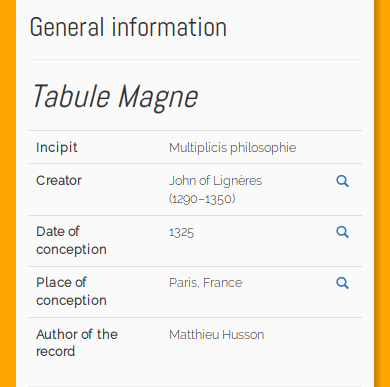
\includegraphics[width=10cm]{Images/Sidebar/metadata-work.png}
	\caption{Metadata display in the sidebar}
\end{figure}

				\subsection{Data struture}\label{data-struture}

The data produced by the \texttt{getMetadataTable()} method is always structured the same way in order to correctly generate the sidebar using the template \texttt{sideMetadata.html.twig}.

\begin{lstlisting}
$metadata = ["entity" => $entityName // index name that will be used to construct an Elastisearch query
         "title" => $title, // text to display in the upper part of the sidebar
        ("subtitle" => $subtitle), // facultative
         "field name" => ["values" => ["text to display"],
                  "search" => ["json" => ["query to send to ElasticSearch"],
                           "hover" => "text to display when hovering the magnifier"],
                       "title" => ["title of the query"]],
         "other field" => ["values" => [["html" => "text to display", // when text must be a link
                         "id" => "id of the entity for the link",
                         "path" => "path name to construct link"]],
                   "search" => ["json" => [],// no magnifier when this array is empty
                        "hover" => ""],
                        "title" => []]
];
\end{lstlisting}

Each key of the array (except for the key \texttt{entity}) corresponds to a field that is going to appear in the sidebar. The upper part of the sidebar is filled with the keys \texttt{"title"} and \texttt{"subtitle"} (not required), and for the part in the white insert, each key constitutes the text that is going to appear as field name.

To each of these keys is attached an associative array defining how the metadata related to these fields are going to be displayed. Each key referes to something specific :
\begin{itemize}
	\item  \textbf{values} : the text in \texttt{html} that is going to appear next to the field name. In the array associated to this key, can be added an array if the text is going to be a link~:
	\begin{itemize}
		\item \textbf{html} : text to display
		\item \textbf{id} : id of the entity in order to build the link
		\item \textbf{path} : path of the page to redirect to 
	\end{itemize}
	\item \textbf{search} : data used for generating the magnifier (i.e.~redirecting to the search page for more related items). To this key is attached an other associative array~:
	\begin{itemize}
		\item \textbf{json} : query in the DSL language of ElasticSearch. Not all the query is needed, only the \texttt{query} part. The \texttt{source}, \texttt{size}, etc are generated after that.
		\item \textbf{hover} : text that is going to appear when hovering the magnifier, which is a description of the query
		\item \textbf{title} : title of the query that will appear in the result page
	\end{itemize}
\end{itemize}

The keys \texttt{values}, \texttt{json} and \texttt{title} are associated to an array because some fields can have several values to display, for instance is a work has multiple creators. For example, if a primary source is written in two different scripts, the metadata associated to the ``script field'' will look like this~:

\begin{lstlisting}
["scripts" =>
   ["values" =>
       ["<span class='mainContent'>Latin</span>",
        "<span class='mainContent'>Gothic</span>"],
    "search" =>
       ["json" =>
           ['["bool":["must"=>[[["match"=>["original_texts.script.id"=>85}}]]}}',
            '["bool":["must"=>[[["match"=>["original_texts.script.id"=>46}}]]}}'],
        "hover" =>"Find all primary sources written in the same script",
        "title" => 
           ["All primary sources written in latin",
            "All primary sources written in gothic"]
     ]
 ];
\end{lstlisting}

				\subsubsection{String formatting}\label{string-formatting}

The text that is going to be displayed is formatted thanks to the \texttt{toPublicString} and \texttt{toPublicTitle} methods~:
\begin{itemize}
	\item  \texttt{toPublicString} is used when the information will be displayed as metadata (i.e.~in the record page of an original item, the name of the work of this item will be formatted with this method)~;
	\item \texttt{toPublicTitle} is used when the information will be displayed as main content (i.e.~in the record page of a work, the name of the work will be formatted with this method).
\end{itemize}

The \texttt{getTpaq()} methods returns for each entity associated with a tpq and a taq date, a correctly formatted date, for example :
\begin{itemize}
	\item if \texttt{tpq} = 1245, and \texttt{taq} = 1325 ==\textgreater{} ``1245---1325''
	\item if \texttt{tpq} = 1325, and \texttt{taq} = 1325 ==\textgreater{} ``1325''
\end{itemize}

				\subsubsection{Managing missing information}\label{managing-missing-information}

If an information is missing, (for example, if the current entity doesn't have place associated with it), several layout options are available :
\begin{itemize}
	\item textbf{\emph{Not showing the field at all}} : the key for this field must not appear in the array of metadata, or the array associated to the \texttt{values} key must be lefted empty.
\end{itemize}

\begin{lstlisting}
// the field translator must appear only if there is one
if ($work->getTranslator()){
    $metadata["translator"] = $metadataTable;
    $metadata["translator"]["values"][] = $work->getTranslator()->toPublicString();
}
\end{lstlisting}

\begin{itemize}
	\item \textbf{\emph{Showing the field with a string indicating the missing information}} : in the array associated to the \texttt{values} key, a string can be set when there is no information available for the current field. It must be encapsulated in a \texttt{\textless{}span class="noInfo"\textgreater{}\textless{}/span\textgreater{}} tag.
\end{itemize}

\begin{lstlisting}
// if there is no incipit, display "Missing incipit"
$incipit = $work->getIncipit() ? $work->getIncipit() : "<span class='noInfo'>Missing incipit</span>";
\end{lstlisting}

\begin{itemize}
	\item \textbf{\emph{Keeping the field empty of information}} : when the array of the \texttt{values} key is lefted with an empty string in it, the template of the sidebar will automatically display \texttt{\textless{}span class="noInfo"\textgreater{}No information provided\textless{}/span\textgreater{}}
\end{itemize}

\begin{lstlisting}
// if there is no historical actors, set the values to be [""]
$values = count($actors) != 0 ? [] : [""];
\end{lstlisting}


				\subsubsection{Pie chart}\label{pie-chart}

A pie chart can be displayed a the bottom of the sidebar when creating a key named \texttt{visualisation} in the metadata array, filled with an associative array defining a title and a dataset for the chart.

\begin{lstlisting}
$metadata["visualization"] = [
    "title" => "Title of the visualisation"
    "data" => [["category" => "cat1", "value" => 7],["category" => "cat2", "value" => 4],[...]]
];
\end{lstlisting}

\begin{figure}[H]
	\centering
	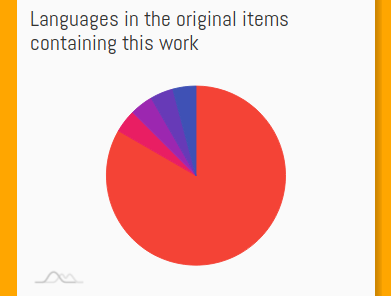
\includegraphics[width=10cm]{Images/Sidebar/pie-work.png}
	\caption{Pie chart at the bottom of the sidebar}
\end{figure}

			\subsection{Sidebar template}\label{sidebar-template}

The sidebar is opened with a click on a toolbar icon, and closed when clicked outside the sidebar. The javascript allows to switch between two states that are defined in the public CSS stylesheet : when opened, the classes \texttt{open-toolbar} and \texttt{open-sidebar} are added to the element of the sidebar in order to appear on the page.

\begin{lstlisting}
$(document).ready(function(){
    // open the sidebar on a toolbar item
    $('.toolbarItem>span').click(function(){
        let id = $(this).attr('id');

        $("#sidebar").attr("isOpen", "true");
        switchSidebar();
        let sideContent = "side-"+id;
        $('.backgroundSidebar').hide();
        $('#'+sideContent).show();
    });

    // close the sidebar when clicked outside the side bar
    $(document).click(function (e) {
        let thatTarget = $(event.target);
        // if the clicked target is not a child of sidebar AND sidebar is open
        if (!thatTarget.closest('#sidebar').length && $("#sidebar").attr('isOpen') === "true"){
            $("#sidebar").attr("isOpen", "false");
            switchSidebar();
        }
    });

    function switchSidebar() {
        if ($("#sidebar").attr("isOpen") === "false") {
            $("#sideBorder, #toolbar").removeClass("open-toolbar");
            $("#innerSidebar").removeClass("open-sidebar");
        } else {
            $("#sideBorder, #toolbar").addClass("open-toolbar");
            $("#innerSidebar").addClass("open-sidebar");
        }
    }
});
\end{lstlisting}

		\section{Search interface}\label{search-interface}

The search page serves for now two purposes~:
\begin{itemize}
	\item allowing the user to perform full-text queries, only on the entities \textbf{work}, \textbf{primary source} and \textbf{original item},
	\item displaying the related items when clicking on a magnifier in the sidebar of a entity record.
\end{itemize}

The queries are performed on the ElasticSearch database through an AJAX call : TODO when launching in production, the requested server (from \texttt{localhost} to \texttt{dishas.obspm}) will change. The variable to be modified to make this change is located in the \texttt{myElasticSearch.js}~:

\begin{lstlisting}
function generateUrl(query="", index="", from = 0, size = 10000, server="localhost:9200", http="http") { ... }
\end{lstlisting}

The retrieved results from this call are then formatted to be displayed in a DataTable thanks to the \texttt{TAMASListTableTemplate} objects. Those templated are defined with the \texttt{getPublicObjectList()} in the entity repositories.

			\subsection{Data structure : TAMASListTableTemplate}\label{data-structure-tamaslisttabletemplate}

The objects of the class \texttt{TAMASListTableTemplate} defines for each field (i.e.~column) of an entity, how the information is going to be presented inside the DataTable. For instance, the template of a work title will defined that the text is going to be in \emph{italic}, \href{}{redirect} to the page of the concerned work and that the string ``Unknown title'' will be displayed if the information is missing.

The \texttt{getPublicObjectList()} is defined as follows :

\begin{lstlisting}
public function getPublicObjectList()
    {
        $fieldList = [
            new TAMASListTableTemplate(
                'name of the key where the information in the array of result will be located',
                'Column title for this field',
               ['class'=>['array of CSS classes to style the text'],
                'path' => 'defined if a the text is a link',
                'id' => 'name of the key where the id in the results is located'],
                'unknown' => 'text to display if the information is missing',
                'fields needed to display this field, correspond to the `_sources` in a ElasticSearch query'
        )];

        return $fieldList;
    }
\end{lstlisting}

Each column needs its template, each entity combining between 5 and 10 templates. A template object can be defined with a certain number of properties~:

\begin{itemize}
	\item \textbf{Name}~: provides the location in an array where DataTable will find the information to display
	\item \textbf{Title}~: corresponds to the column label associated with the information
	\item \textbf{Properties}~: defines how the cell content will be formatted~:
	\begin{itemize}
		\item \textbf{class} (will surround the text in a \texttt{\textless{}span class="\_\_"\textgreater{}\textless{}/span\textgreater{}})~:
		\begin{itemize}
			\item \textbf{\emph{list}} : to indicate that multiple values can be displayed in the same cell
			\item \textbf{\emph{number}} : in order to align the text to the right
			\item \textbf{\emph{title-italic}} : to style the text of the cell in italic
		\end{itemize}
		\item \textbf{path} + \textbf{id}~:
		\begin{itemize}
			\item \textbf{\emph{path}} : routing path to generate a link
			\item \textbf{\emph{id}} : location of the id in the result object
		\end{itemize}
	\end{itemize}
	\item \textbf{Source} : defines which fields will appear in the elasticsearch response corresponding to the fields that are added to the array associated with the key ``source'' in the query (multiple fields can be added for a single column with ``+'')
\end{itemize}

\begin{lstlisting}
// Field "Work" of an original item defining how the work titles will appear
new TAMASListTableTemplate(
    'work',
    'Work',
    ['class' => ['title-italic'], 'path' => 'tamas_astro_viewWork', 'id' => 'work.id'],
    '', // ifOnly is not used in the public interface
    'work.default_title+work.id'
)
\end{lstlisting}

			\subsection{Specific functions}\label{specific-functions}

The functions and variables used to create the search interface are located in several files~:
\begin{itemize}
	\item \texttt{publicResult.html.twig} : twig template for the result page
	\item \texttt{myElasticSearch.js} : functions to build queries, to retrieve data from response or generate URL
	\item \texttt{myDataTable.js} : functions related to DataTables
	\item \texttt{mainJavascript} : utility functions
\end{itemize}

The main functions help :
\begin{itemize}
	\item to \textbf{retrieve results} from ElasticSearch
\end{itemize}

\begin{lstlisting}
/**
* This function takes a response from an ajax call to elasticsearch
* and returns an array containing all the results of this query
*
* @param queryResponse : object
* @return {Array}
*/
function retrieveResults(queryResponse) {
    if (typeof queryResponse.hits.hits !== 'undefined') {
        let data = queryResponse.hits.hits; // data is an array of results, but only the value of the key "_source" is needed
        let results = [];

        $.each(data, function (key, value) {
            results.push(value._source);
        });

        return results;
    }
}
\end{lstlisting}

\begin{itemize}
	\item to \textbf{format those results} (using the properties defined in the \texttt{TAMASListTableTemplate})
\end{itemize}

\begin{lstlisting}
/**
* to either return the information associated with a field
* or return a tag indicating missing information
* The properties will defined how the cell content is formatted.
*
* @param text : result values to display inside an array (even if there is only 1 value)
* @param properties : object defined in the template object list (getPublicObjectList)
* @param result : object containing the results send by Elasticsearch
* @returns string
*/
function textDisplay (text, properties=[], result={}){
    let classes = "";
    if (isDefined(properties.class)){ // putting all classes in the same string
        for (let i = 0; i < properties.class.length; i++){
            let className = properties.class[i];
            classes = classes + className;
            classes = i < properties.class.length ? classes + " " : "";
        }
    }

    if (isDefined(text)){
        if (isDefined(properties.path)){
            let id = [selectNodeOfObject(properties.id, result)];
            // selectNodeOfObject will select the id in the result if there is only one id to find,
            // unlike when the cell is supposed to contain a list
            if (isDefined(properties.class) && properties.class.includes("list")){
                // if the cell is supposed to contain a list of links
                // the "text" array looks like : ["text, id, "text", id, ...]
                let texts = [];
                id = [];
                for (let j = 0; j < text.length; j += 2){
                    texts.push(text[j]);
                    id.push(text[j+1]);
                }
                text = texts; // now it looks like ["text","text", ...]
            }
            let linkText = [];
            for (i = 0; i < text.length; i++){
                linkText.push(`<a href="${generateRoute(properties.path, id[i])}">${text[i]}</a>`);
            }
            text = linkText;
        }

        let cellContent = "";
        let cellSummary = "";
        for (i = 0; i < text.length; i++){
            if (i === 0){
                cellContent = classes !== "" ? `<span class="${classes}">${text[i]}</span>` : `${text[i]}`;
            } else {
                cellSummary = cellSummary + `<span class="${classes}">${text[i]}</span>`;
                cellSummary = i < text.length ? cellSummary + "<br/>" : "";
            }
        }
        if (text.length > 1){ // if there is multiple data to display, put it in a summary
            let Nrecord = text.length > 2 ? "s" : "";
            let summary = `<summary class="mainContent">
                                        ${text.length-1} <span style="font-variant: small-caps">more record${Nrecord} </span>
                                        <span style="font-size: 10px">▼</span>
                                    </summary>`;
            cellContent = `${cellContent}<details>${summary}${cellSummary}</details>`;
        }
        return cellContent;
    } else { // if the key doesn't exist in the array of results => missing information
        if (isDefined(properties.unknown)){
            return `<span class='noInfo'>${properties.unknown}</span>`;
        }
        return "<span class='noInfo'>No information provided</span>";
    }
}
\end{lstlisting}

\begin{itemize}
	\item to \textbf{display those results} in a \texttt{DataTable}
\end{itemize}

\begin{lstlisting}
/**
* This function generates an entire Datatable of results retrieved from a query to elasticsearch
* on the given index for the filters given as parameter query
*
* it generates by default a query of a size 10000, from 0
*
* @param index string : label of an entity (ex : "primary_source")
* @param query object : the filters of the query (ex: {"match":{"id":"5"}})
*                      => the value associated with the key "query" in the query language of elasticsearch
* @param queryTitle string : title detailing the query in natural language (EX => "All original items kept in the British Library")
* @param queryTerm string : terms used to filter the results
* @param from int : the number of results from which the query starts
* @param size int : number of results wanted in the response
* @param generateHeader bool : defines if the header is generated or not
* @return url : url of the query
*/
function generateResultTable(index, query, queryTitle="", queryTerm="", from=0, size=10000, generateHeader=true) {
    let fieldList = fieldLists[index];
    let dataStructure = generateDataStructure(fieldList);
    let sourceFields = generateSources(fieldList, true);

    // generates columns labels
    generateColumnHeader("results", fieldList)

    // generates URL in order to make an ajax call
    let url = generateUrl(query, index, from, size);

    // defining the function formatting the response of an elasticsearch ajax call
    // into an array of results ready to be displayed by DataTable
    let formatData = function (queryResponse){
        let results = retrieveResults(queryResponse);
        for (let result of results){
            let i = 0;
            for (let field of fieldList){
                // field.name is the key where DataTable is going to search for the value to fill the cells of one specific column
                // textDisplay() returns the value that is going to be displayed in the cell :
                // 		- the text correctly formatted (according to the field.properties)
                // 		- OR no information provided (if there is no value in the result array)
                // selectNodeOfObject() returns the value of the node in the array of result
                // corresponding to string given as first argument
                result[field.name] = textDisplay(selectNodeOfObject(sourceFields[i], result, field.properties), field.properties, result);
                i++;
            }
        }
        return results;
    };

    if (generateHeader){
        // generates a header for the current query
        generateSearchHeader(index, queryTitle, queryTerm);
    }

    let table = $('#results').DataTable({
        "ajax": {
            "url": url, // url on which the query is done
            cache: true, // mandatory in order to send the query without wildly added parameters
            "dataSrc": formatData // variable containing the function formatting the results in order to fill the DataTable
        },
        "columns": dataStructure, // specify where DataTable will find information associated with each fields
        });
    return url;
}
\end{lstlisting}

		\section{Bread crumbs and table editions}\label{bread-crumbs-and-table-editions}

			\subsection{Bread crumbs}\label{bread-crumbs}

The breadcrumbs allows the user to find his way around the front office, it indicates at which level of the site hierarchy they are located. The javascript code to generate them takes as argument the name of the current node, i.e.~the name of the page, and it reconstructs the page tree structure to get there.

\begin{lstlisting}
// define an array to contain the dependance tree of the current page
let nodeTree = [];
nodeTree.push(currentNode);
let node = currentNode;

for (nav of nodeTree){
    if (navigation[nav]){ // navigation contains all the nodes associated with their parent node
        nodeTree.push(navigation[nav]);
    }
}

if (!(nodeTree.length <= 1)){
    // reverse the order of the array to put the greater parent first
    nodeTree.reverse();

    // create a breadcrumb for each node of the nodeTree object
    for (let l = 0; l < nodeTree.length ; l++){
        node = nodeTree[l];
        // set the pictogram image of the current node
        let picto = "{{ asset('img/pictograms/'~'INTERFACENAME'~'.png') }}";
        picto = picto.replace("INTERFACENAME", node);

        if (properties[node]["path"] !== ""){
            // generate a route for the current node
            let route = Routing.generate(properties[node]["path"]);
        }

        $(".breadcrumb-icons").append(`<div class="col-md-1 picto-bundle">
                                        <a href="${route}" title="${properties[node]["hover"]}">
                                            <div class="picto-background ${currentNode}">
                                                <img class="picto-size"
                                                     src="${picto}"
                                                     alt="${properties[node]["title"]} pictogram">
                                            </div>
                                        </a>
                                    </div>
                                    <div class="col-md-1 chevron">
                                        <span class="glyphicon glyphicon-chevron-right"></span>
                                    </div>`);
    }
}
\end{lstlisting}

			\subsection{Related table editions}\label{related-table-editions}

The relation of the edited texts and the original texts are modelled in a graph structure in order to limit aberration and loops (preventing an edition to be based on an edition that is itself based upon this edition), and to display graph visualisations for the editions. With the aim of gathering all the editions that were based on one particular original item, including the \emph{indirect} ones (type B editions), it is necessary to use the graph structure.

\texttt{DISHAS/src/TAMAS/AstroBundle/Repository/OriginalTextRepository.php}

\begin{lstlisting}
/**
* getAllEditedTexts
*
* this method returns an array of the editions of an original item, including indirect editions (type B)
* 
* @param \TAMAS\AstroBundle\Entity\OriginalText $originalText
* @return array
*/
public function getAllEditedTexts(\TAMAS\AstroBundle\Entity\OriginalText $originalText)
{
   if (! $originalText)
      return [];

   $editedTextRepo = $this->getEntityManager()
      ->getRepository(\TAMAS\AstroBundle\Entity\EditedText::class);

   $dependanceTree = $editedTextRepo->getDependanceTree();
   $graph = new \TAMAS\AstroBundle\DISHASToolbox\Graph\TAMASGraph();
   $graph->loadJSONTree($dependanceTree);

   $origItemId = $originalText->getId();

   $originalId = 'o' . $origItemId; // the id of the original item is preceded by "o" in the graph tree
   $original = $graph->getNode($originalId); // find the node corresponding
   $editedTexts = $original->getAncestors(); // find the edited texts related to this node

   $editions = [];
   foreach ($editedTexts as $editedText){
      // fill the array with all the edited texts corresponding to the id
      $editions[] = $editedTextRepo->findBy(['id' => str_replace("e", "", $editedText->getLabel())])[0];
   }

   return $editions;
}
\end{lstlisting}

\clearemptydoublepage

\chapter{\label{AmCharts}Introduction à la bibliothèque \eng{AmCharts}}

This page is a general introduction to the charts javascript library AmCharts in its version V4. An extensive documentaion and API can be found \href{https://www.amcharts.com/docs/v4/}{here}, demos of all the charts that can be made can be found \href{https://www.amcharts.com/demos/}{here} and tips to customize chart can be found \href{https://www.amcharts.com/t/tips/}{there}.

		\section{Instantiating a chart}\label{instantiating-a-chart}

			\subsection{Modules}\label{modules}

AmCharts allows to create several kind of charts. Depending on the one you wish to create, you will need to import several modules from the library. In all cases, you will need the main module \texttt{am4core} (which should always comes first) and an other module corresponding to the type of chart~: either the \texttt{am4charts} for all the \emph{regular} charts, or \texttt{am4maps} for map visualisations.

Some kind of charts requires additionnal plugins like force-directed graphs (\texttt{forceDirected}) or maps that need to import some geodata to display a background map (\texttt{worldLow}).

On top of that, you can import modules for \href{https://www.amcharts.com/docs/v4/getting-started/using-javascript/\#Assets}{setting assets} like translations or themes that will define behaviors and color set of the charts.

\begin{lstlisting}
<script src="https://www.amcharts.com/lib/4/core.js"></script>
<script src="https://www.amcharts.com/lib/4/charts.js"></script>
<script src="https://www.amcharts.com/lib/4/maps.js"></script>
<script src="https://www.amcharts.com/lib/4/geodata/worldLow.js"></script>
<script src="https://www.amcharts.com/lib/4/themes/animated.js"></script>
\end{lstlisting}

			\subsection{Creating a chart}\label{creating-a-chart}

The \texttt{create()} function is always first used to add new instances to your HTML page. It takes two arguments~:

\begin{itemize}
	\item The \textbf{tag id} of the \texttt{html} element in which is going to contain the chart (the element must already exist in your DOM, the function will not create it)~;
	\item The \textbf{type of chart}, \emph{i.e.} the class reference.
\end{itemize}

\begin{lstlisting}
var chart = am4core.create("chartdiv", am4charts.XYChart);
\end{lstlisting}

				\subsubsection{Combining multiple charts}\label{combining-multiple-charts}

Is it possible to put several charts in the same \texttt{html} element. To do that you only need to create first a \href{https://www.amcharts.com/docs/v4/concepts/svg-engine/containers/}{container} in which you will create charts instances~:

\begin{lstlisting}
var container = am4core.create("chartdiv", am4core.Container);
var mapChart = container.createChild(am4maps.MapChart);
var XYChart = mapChart.chartContainer.createChild(am4charts.XYChart);
\end{lstlisting}

				\subsubsection{Configuration~: object/JSON approachs}\label{configuration-objectjson-approachs}

There are two way of setting up the parameters and data for the charts~: either a \href{https://www.amcharts.com/docs/v4/getting-started/basics/\#Using_JSON}{\textbf{JSON-based}} approach, or an \href{https://www.amcharts.com/docs/v4/getting-started/basics/\#Object_based_approach}{\textbf{object-based}} approach. Object approach is more readable and less prone to bug whereas JSON approach, being fundamentally a string, can be stored in a database or load dynamically with AJAX.

The rest of this introduction will only give examples with the object approach but you can find more information \href{https://www.amcharts.com/docs/v4/concepts/json-config/}{here} on the JSON way. Object-based only means that the chart is treated as an object whose properties we're going to change/call.

		\section{Anatomy of a chart}\label{anatomy-of-a-chart}

A chart is mainly composed of two elements~: the \textbf{``\emph{frame}''} and the ``\textbf{\emph{shapes}}'' representing the data~:

\begin{itemize}
	\item The \emph{frame} is, in most cases, composed of two \texttt{axes} defining the structure of the chart.
	\item The data can be displayed in different \emph{shapes} depending of the type of chart~: columns, bubbles, points, line, etc. Whatever its shape, data is an instance of one or several \texttt{series}.
\end{itemize}

			\subsection{\href{https://www.amcharts.com/docs/v4/concepts/axes/}{Axes}}\label{axes}

Axes are the structure of the chart~; they are specially fundamental to XYChart and some other type of charts. The axes determines how the data is going to be spread out through out the chart.

The axes can be of mainly two types~:

\begin{itemize}
	\item \href{https://www.amcharts.com/docs/v4/concepts/axes/category-axis/}{\textbf{Category axis}}~: used to position data items on text-based categories. For example, for a dataset detailling the number of folio per manuscript, the category axis would represent all the manuscripts.
	\item \href{https://www.amcharts.com/docs/v4/concepts/axes/value-axis/}{\textbf{Value axis}}~: used to position data items on a numeric scale. In our previous example, it would represent the total number of folios.
	\item Other types of axes~:
	\begin{itemize}
		\item \textbf{Duration axis}
		\item \textbf{Date axis}
	\end{itemize}
\end{itemize}

And, in the case of XYCharts, axes can be horizontal -- or circular in case of some charts like radar -- (\texttt{xAxes}) or vertical (\texttt{yAxes})~; any of them can be a category axis or value axis, and both of them can be of the same type.

				\subsubsection{Creating axes}\label{creating-axes}

To associate axis to a chart, you need to push them to your existing chart like so~:

\begin{lstlisting}
var valueAxis = chart.yAxes.push(new am4charts.ValueAxis());
var categoryAxis = chart.xAxes.push(new am4charts.CategoryAxis());
\end{lstlisting}

				\subsubsection{Configuring axes}\label{configuring-axes}

Most of the appearence parameters and settings can be configured \href{https://www.amcharts.com/docs/v4/reference/axis/}{directly on the axis variable} or with the \href{https://www.amcharts.com/docs/v4/reference/axisrenderer/}{\texttt{renderer} property}~:

\begin{lstlisting}
// define a title for the value axis
valueAxis.title.text = "Number of folios";
// display the axis one the opposite side than the default one
categoryAxis.renderer.opposite = true;
// to set the background grid of the value axis to be transparent
valueAxis.renderer.grid.template.strokeOpacity = 0;
// set the font size of the label from the category axis to 20
categoryAxis.renderer.labels.template.fontSize = 20;
\end{lstlisting}

			\subsection{\href{https://www.amcharts.com/docs/v4/concepts/series/}{Series}}\label{series}

A series is a collection of similar, logically grouped data points, it gathers the configuration defining how the data is going to be displayed.

One series aggregates data you want to have the same properties. Sometimes one series will be enough to display gigantic datasets, but sometimes you will need to provide each data its series in order to specify finely the settings for each one in particular. A series, in a column chart for instance, can be either --- depending on what you want to show --- a group of columns, a single column, a group of cells through out the columns or a single cell.

Each type of chart allows only certain kind of series~: a \texttt{pieSeries} on a \texttt{mapChart} will never be displayed.

Series have two main purposes: - Setting appearance and behavior of a collection of chart items~; - Binding individual chart items to source data.

				\subsubsection{Creating series}\label{creating-series}

To create a new series for your chart, you must proceed as for the axes~:

\begin{lstlisting}
var series = chart.series.push(new am4charts.ColumnSeries());
\end{lstlisting}

				\subsubsection{Configuring series}\label{configuring-series}

You can set configuration for a series either \href{https://www.amcharts.com/docs/v4/reference/series/}{directly} on the series variable or through its \href{https://www.amcharts.com/docs/v4/concepts/series/\#Templates}{\texttt{template} property} (more on templates \href{https://gitlab.obspm.fr/gtopalian/DISHAS/wikis/AmCharts/developper_general_introduction\#templates}{later on})~:

\begin{lstlisting}
// setting width of the stroke
series.strokeWidth = 0;
// setting text appearing when hovering on columns
series.columns.template.tooltipText = "Number of folios in manuscript";
\end{lstlisting}

			\subsection{Additionnal components}\label{additionnal-components}

Inside a chart, you can add several type components like \textbf{SVG shapes}, \textbf{labels}, etc. To create them, you need to push them in your chart container, then you can configure them as you like~:

\begin{lstlisting}
var rectangle = chart.chartContainer.createChild(am4core.Container);
var rectLabel = rectangle.createChild(am4core.Label);
\end{lstlisting}

		\section{Data}\label{data}

			\subsection{\href{https://www.amcharts.com/docs/v4/concepts/data/\#Structure_of_data}{Data structure}}\label{data-structure}

All data, in order to be used by your chart, need it to be formatted as an \textbf{array of objects}~:

\begin{lstlisting}
var msData = [
  {
    "ms": "Latin 10264",
    "folios": 3
  },{
    "ms": "Bav. Lat. 1374",
    "folios": 14
  }
]
\end{lstlisting}

			\subsection{\href{https://www.amcharts.com/docs/v4/concepts/series/\#Binding_to_data}{Binding data}}\label{binding-data}

In order to make your chart use your data, you first need to associate your array to the data property of your chart~:

\begin{lstlisting}
chart.data = msData;
\end{lstlisting}

With this line, when we will set data properties to our chart series, it will know automatically where to find the information it needs. You can also bind a dataset to a \href{https://www.amcharts.com/docs/v4/concepts/data/\#Series_specific_data}{specific series} for complex layouts.

			\subsection{Using \href{https://www.amcharts.com/docs/v4/concepts/data/\#Data_fields}{data fields}}\label{using-datafields}

Now, the axes and the series that have been earlier create needs to be associated with the data from our array. The \texttt{dataFields} property is a simple object that binds specific field in series, to a data field in data objects~: using \texttt{dataField} the series, as well as the category axis, will know what key in the dataset they are binded to.

\begin{lstlisting}
series.dataFields.categoryX = "ms";
series.dataFields.valueY = "folios";
categoryAxis.dataFields.category = "ms";
\end{lstlisting}

What those lines means is~: for each object in the array of data, the numerical value for the series will be found to the ``folios'' key and the string-based value will be found to the ``ms'' key. The value axis will generate itself according to the maximal value associated with the series to display, but the category axis needs to know which labels to show.

\textbf{NB}~: for each kind of chart, the syntax might vary. You will find more details on that in the numerous examples in the \href{https://www.amcharts.com/demos/}{demos}.

				\subsection{Using \href{https://www.amcharts.com/docs/v4/concepts/data/\#Property_fields}{properties fields}}\label{using-propertiesfields}

The \texttt{dataFields} property only holds information that is needed for the chart to be displayed, additionnal information can be binded to the chart to customize it further~: \texttt{propertyFields} are the way to tie chart element's properties to data.

Let's say some fields were added to your dataset like that~:

\begin{lstlisting}
var msData = [
  {
    "ms": "Latin 10264",
    "folios": 3,
    "color": "#fcba03",
    "url": "https://archivesetmanuscrits.bnf.fr/ark:/12148/cc71999k"
  },{
    "ms": "Bav. Lat. 1374",
    "folios": 14,
    "color": "#fc3103",
    "url": "https://digi.ub.uni-heidelberg.de/diglit/bav_pal_lat_1374"
  }
];
\end{lstlisting}

Pretty much any part of your chart can be customize using information from your dataset with the \texttt{propertiesField} property~:

\begin{lstlisting}
// make column labels a link
categoryAxis.renderer.labels.template.propertyFields.url = "url";
// colour the columns
series.columns.template.propertyFields.fill = "color";
\end{lstlisting}

				\subsubsection{Using \href{https://www.amcharts.com/docs/v4/concepts/data/\#Using_dummy_data_}{dummy data}}\label{using-dummydata}

You can bind any data of your choice to a chart item using its \texttt{dummyData} property~: it is a sort of storage container to put anything you want in it, without affecting the overall behavior of your chart.

It can be very useful when you will need to customize your chart creating tailored function using \href{https://www.amcharts.com/docs/v4/concepts/event-listeners/}{event listeners} or \href{https://www.amcharts.com/docs/v4/concepts/adapters/}{adapters}~: it can become handy if you are dynamically generating data you want to access later on, for instance to bind behavior for two distinct events.

		\section{Appearance configuration}\label{appearance-configuration}

			\subsection{\href{https://www.amcharts.com/docs/v4/concepts/list-templates/}{Templates}}\label{templates}

Practically all of the charts components have a \texttt{template} property~: it is some kind of pattern for the layout and behavior of specific parts of your chart. Using templates, you can, for example, set that all filling colors of columns to be half transparent or for all axis labels to become green when clicked on~:

\begin{lstlisting}
// Half transparency of the columns
series.columns.template.fillOpacity = 0.5;
// Green labels
valueAxis.renderer.labels.template.events.on("hit", function(ev) {
  valueAxis.renderer.labels.template.fill = "green";
});
\end{lstlisting}

Templates can be modified dynamically using DOM events, which is not the case with data values (associated with \texttt{dataFields})~: to change the values your chart is using, you will need either to \href{https://codepen.io/segolene-albouy/pen/rExamo}{switch datasets} or use \href{https://www.amcharts.com/docs/v4/concepts/data/\#Incremental_updates}{incremental loading}).

AmCharts is an incredibly customisable library~: if you would like to change any aspects of your chart, by browsing through the properties of the element you want to modify in the \href{https://www.amcharts.com/docs/v4/reference/}{API}, you will surely find something to suit your desires.

			\subsection{\href{https://www.amcharts.com/docs/v4/concepts/colors/}{Colors}, percentage, etc.}\label{colors-percentage-etc.}

To unlock all methods applicable to colors and percentages, you will need to use special Amcharts functions. The \texttt{color()} method takes only one argument of color and transform it into an object that can be later on \href{https://www.amcharts.com/docs/v4/reference/color/\#Methods}{modified}. The same is true for \href{https://www.amcharts.com/docs/v4/reference/percent/}{\texttt{percent()}} method. To define the color or the percentage of a property~:

\begin{lstlisting}
rectangle.width = am4core.percent(50);
rectangle.background.fill = am4core.color("orange");
\end{lstlisting}

				\subsubsection{\href{https://www.amcharts.com/docs/v4/concepts/series/\#Defining_a_heat_rule}{Heat rules}}\label{heat-rules}

Heat rules defines a property of a chart item that will be bind to a numeric value. Any property is usable, as long as you can define a min and max state like so~:

\begin{lstlisting}
// The higher the value, the wider the column
series.heatRules.push({
    target: series.columns.template,
    property: "width",
    min: 80,
    max: 160
});
\end{lstlisting}

			\subsection{\href{https://www.amcharts.com/docs/v4/concepts/states/}{States}}\label{states}

Any part of the chart can be associated with a \texttt{state} object that holds properties defining how the element will behave when on this particular state. States define alternative properties that will override ``\emph{normal state}'' properties on certain occasions.

As many other objects in AmCharts, defining state is a two steps process~: first \textbf{creating} the state for a specific element, then \textbf{configurating} it~:

\begin{lstlisting}
var hoverState = series.columns.template.states.create("hover");
hoverState.properties.fillOpacity = 0.9;
\end{lstlisting}

			\subsection{\href{https://www.amcharts.com/docs/v4/concepts/formatters/formatting-strings/}{Formatting text} in labels and tooltips}\label{formatting-text-in-labels-and-tooltips}

				\subsubsection{\href{https://www.amcharts.com/docs/v4/concepts/formatters/formatting-strings/\#Visual_formatting}{Font styling}}\label{font-styling}

Text styling options are always contained in \texttt{{[}square brackets{]}}. It works like HTML tag so each opening bracket should be closed with a closing bracket (\texttt{{[}/{]}}), but an other opening bracket will act as a closing one for one opened earlier.

Some styling have an already \href{https://www.amcharts.com/docs/v4/concepts/formatters/formatting-strings/\#Visual_formatting}{implemented syntax} in AmCharts, but you can use any CSS property~:

\begin{lstlisting}
rectLabel.text = "[bold]Work diffusion[/] :\n the example of the [font-style: italic]Tabule Magne[/]";
\end{lstlisting}

				\subsubsection{Accessing \href{https://www.amcharts.com/docs/v4/concepts/data/\#Placeholders_in_on_screen_text}{data values}}\label{accessing-data-values}

Is it possible to display data in labels with the \texttt{\{curly brackets\}} notation. Depending on \href{https://www.amcharts.com/docs/v4/concepts/formatters/formatting-strings/\#Placeholder_examples}{what you write} in your brackets, the parser (or the ``formatter'' to use AmCharts taxonomy) will try to find matching data in your dataset. You can either use the name of a key in your dataset, or the class reference of the data~:

\begin{lstlisting}
series.columns.template.tooltipText = "Numbers of [{color}]folios[/] in {ms} : \n {valueY}";
\end{lstlisting}

You can even perform some data computing on your numeric values with the formatter using \href{https://www.amcharts.com/docs/v4/concepts/formatters/formatting-strings/\#Placeholders_for_numeric_values}{modifiers} such as \texttt{sum} or \texttt{count}.

				\subsubsection{Using HTML}\label{using-html}

You can also display any HTML elements in your \href{https://www.amcharts.com/docs/v4/tutorials/tooltips-with-rich-html-content/}{tooltips} and \href{https://www.amcharts.com/docs/v4/reference/label/\#html_property}{labels} using the \texttt{html} or \texttt{tooltipHTML} property :

\begin{lstlisting}
rectangle.tooltipHTML = '<span style="font-variant: small-caps;">Regarding folio quantity in manuscript</span>';
\end{lstlisting}

		\section{Additionnal features}\label{additionnal-features}

Satellite elements can be instantiated by creating a new object of their class, they will behave accordingly to their normal use but you can completely divert their utility

			\subsection{\href{https://www.amcharts.com/docs/v4/concepts/chart-cursor/}{Cursors}}\label{cursors}

Cursors are only available for XY charts and radar charts~: they allow to add interactivity to charts as well as providing zoom modalities.

\begin{lstlisting}
chart.cursor = new am4charts.XYCursor();
\end{lstlisting}

By default, cursors, when moving on the chart, display two crossing lines ending with tooltips to better pinpoint and understand the data, but all of this can be disabled or modified. You can as well, add some cursor behaviors to allow \href{https://www.amcharts.com/docs/v4/concepts/chart-cursor/\#Zooming_panning}{zooming and panning}~:

\begin{lstlisting}
chart.cursor.behavior = "selectX";
\end{lstlisting}

			\subsection{\href{https://www.amcharts.com/docs/v4/reference/scrollbar/}{Scrollbar}}\label{scrollbar}

A scrollbar is associated to an axis of the chart and allows to zoom in it. Is it possible to push series in it to display a \href{https://www.amcharts.com/docs/v4/chart-types/xy-chart/\#Scrollbar_with_preview}{preview} of the value of your chart, even to \href{https://www.amcharts.com/docs/v4/tutorials/scrollbar-only-xy-chart/}{treat it as a chart} in itself.

\begin{lstlisting}
var scrollbarX = new am4charts.XYChartScrollbar();
scrollbarX.series.push(series);
chart.scrollbarX = scrollbarX;
\end{lstlisting}

			\subsection{\href{https://www.amcharts.com/docs/v4/concepts/legend/}{Legends}}\label{legends}

A legend, when created, will automatically display the series that are associated to your chart. When clicking of the items of the legend, corresponding series disappear, giving possibilities to vary the visualization to the user.

In the case of our manuscript chart, adding a legend is not very insightful, because our data is contained in an unique series representing all the columns, which colors were assigned individually. If we wanted to display a matching legend, we would need to build a \href{https://www.amcharts.com/docs/v4/concepts/legend/\#Adding_custom_items}{custom legend}.

\begin{lstlisting}
chart.legend = new am4charts.Legend();
\end{lstlisting}

			\subsection{\href{https://www.amcharts.com/docs/v4/concepts/event-listeners/}{Events listeners}}\label{events-listeners}

Event listeners allows to bind custom functions to any action perform on a chart element. Each part of the chart has a list of events tied to variables that can be accessed and modified when the event is triggered.

Two kind of functions can be associated to the events~:
\begin{itemize}
	\item \texttt{on()}~: any time the event happens~;
	\item \texttt{once()}~: the first time the event happens.s
\end{itemize}

\begin{lstlisting}
chart.cursor.events.on("selectended", function(ev) {
  var range = ev.target.xRange;
  var axis = ev.target.chart.xAxes.getIndex(0);
  var from = axis.getPositionLabel(axis.toAxisPosition(range.start));
  var to = axis.getPositionLabel(axis.toAxisPosition(range.end));
  alert("Selected from " + from + " to " + to);
});
\end{lstlisting}

The syntax for setting custom functions is always the same~:

\texttt{\{chartName\}.\{elementName\}.events.{[}on/once{]}("\{eventName\}", function(args) \{...\});}

Some events are universal to any type of element, as \texttt{hit}, when the user is clicking or tapping on a touch screen.

		\section{Demos}\label{demos}

			\subsection{Our manuscript chart}\label{our-manuscript-chart}

Here is the chart that was made during this introduction : \href{https://codepen.io/segolene-albouy/pen/LwRBdg}{Number of folios in manuscript}.

\begin{figure}[H]
	\centering
	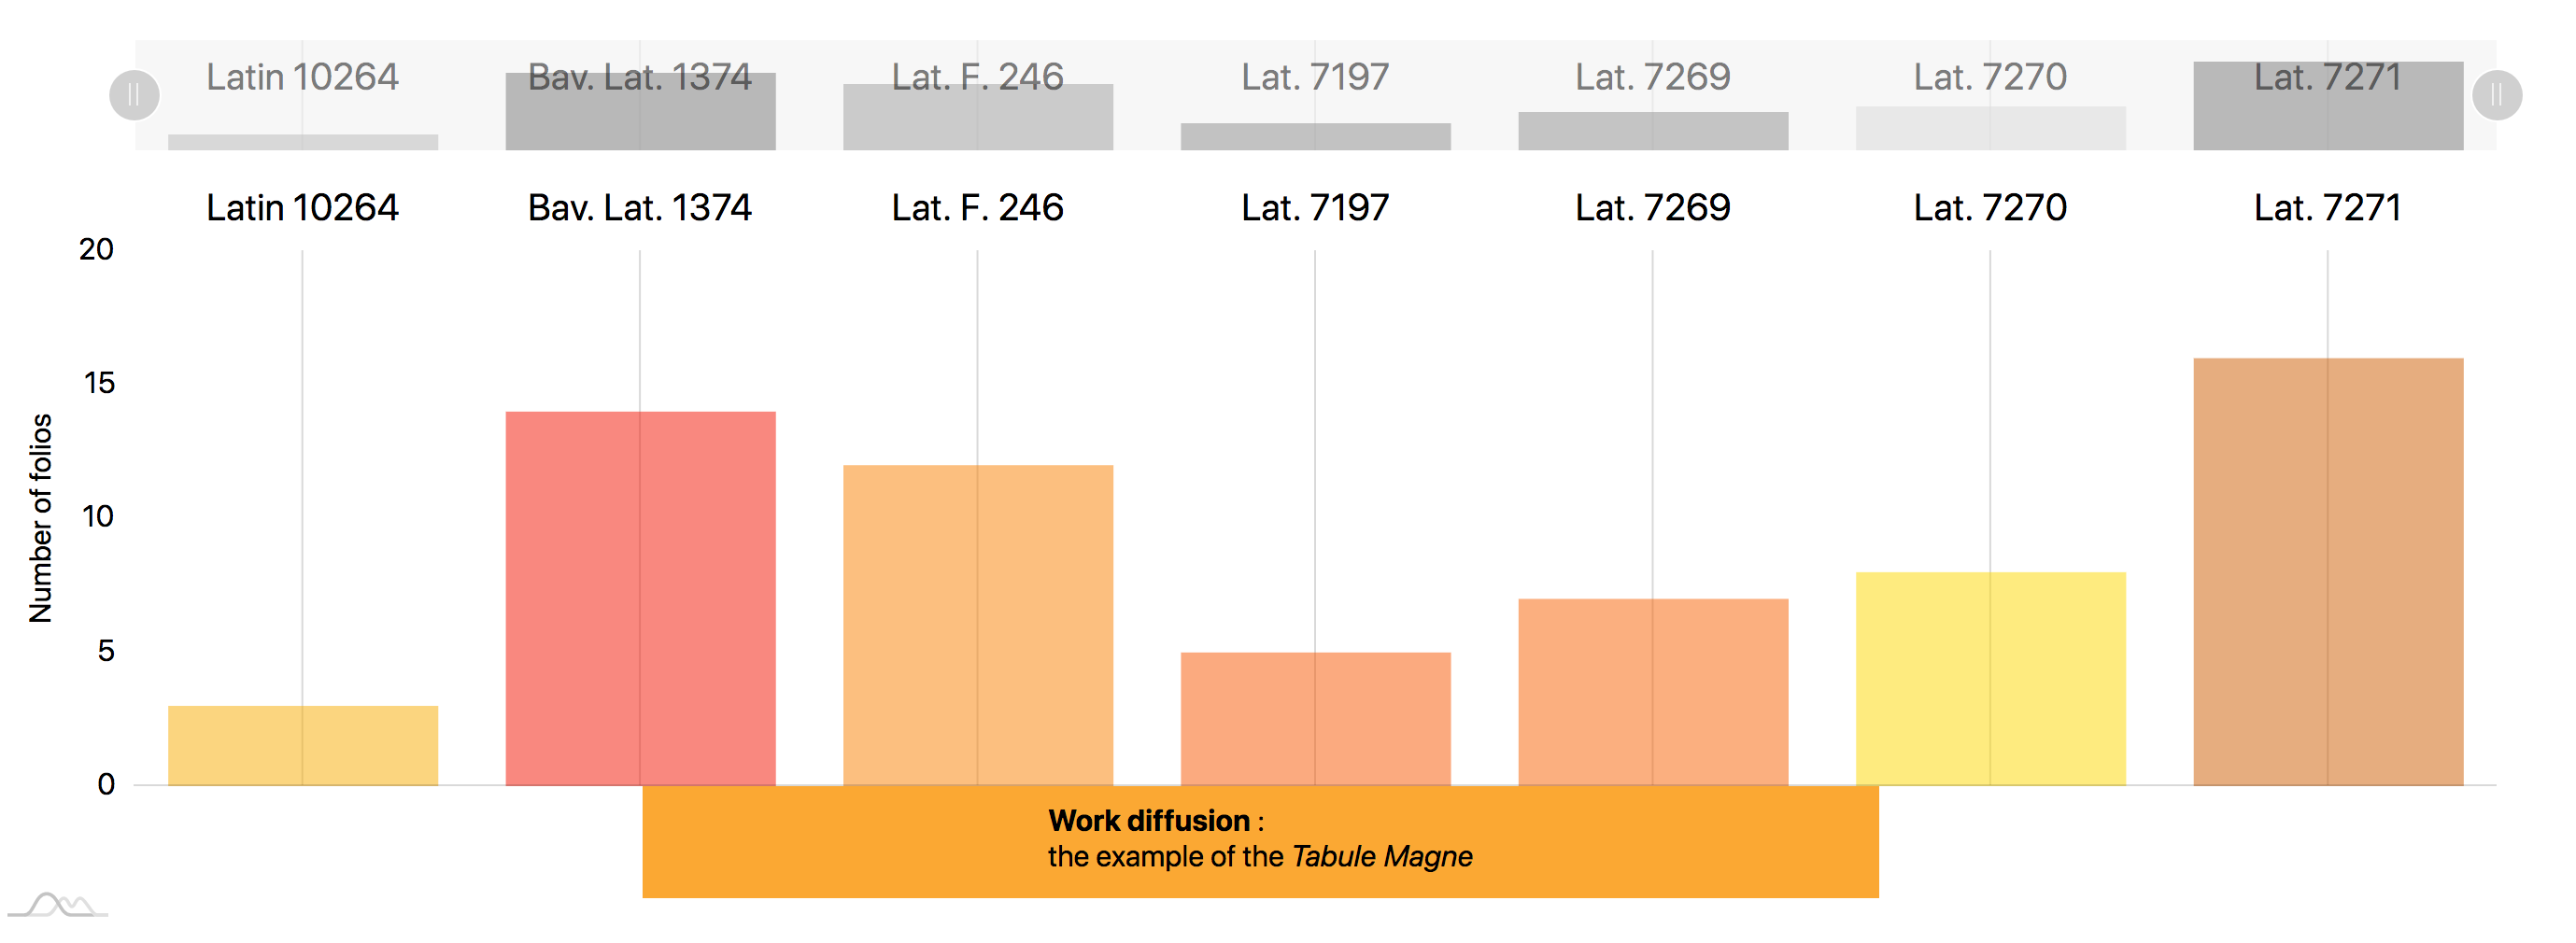
\includegraphics[width=15cm]{Images/Visualisations/Chart-tutoriel.png}
	\caption{Chart made during the AmCharts tutorial}
\end{figure}

			\subsection{Examples in DISHAS}\label{examples-in-dishas}

\begin{itemize}
	\item Primary source~: \href{https://codepen.io/segolene-albouy/pen/rExamo}{dynamic bar chart}
	\item Historical sources~: \href{https://codepen.io/segolene-albouy/pen/KOKBwL}{historical map}
\end{itemize}

\clearemptydoublepage

	\printacronyms[title=Liste des acronymes,toctitle=Acronymes]
	
	\backmatter
	\listoffigures
	\tableofcontents
	
\end{document}